\documentclass[12pt,a4paper]{report}
\usepackage{newtxtext,newtxmath}
\usepackage{setspace}
\usepackage{indentfirst}
\usepackage{geometry}
\usepackage{caption}
\usepackage{graphicx}
\usepackage{fancyhdr}
\usepackage{titlesec}
\usepackage{longtable}
\usepackage[utf8]{inputenc}
\usepackage{amsmath}
\usepackage{subcaption}
\usepackage{booktabs}
\usepackage{float}
\usepackage{siunitx}
\usepackage{array}
\usepackage{multicol}
\usepackage[numbers,sort&compress]{natbib}
\usepackage{hyperref}
\usepackage{microtype}
\usepackage{tabularx}



\geometry{
  left=3cm,
  right=1.5cm,
  top=2cm,
  bottom=2cm
}

\setlength{\parindent}{1.25cm}
\setlength{\parskip}{0pt}
\onehalfspacing
\raggedbottom
\sloppy

\titleformat{\chapter}[hang]
  {\normalfont\fontsize{14}{21}\bfseries}{\thechapter}{1em}{}
\titlespacing*{\chapter}{0pt}{0pt}{1em}

\titleformat{\section}[hang]
  {\normalfont\fontsize{12}{18}\bfseries}{\thesection}{1em}{}
\titlespacing*{\section}{0pt}{1em}{1em}

\titleformat{\subsection}[runin]
  {\normalfont\fontsize{12}{18}\bfseries}{\thesubsection}{1em}{}
\titlespacing*{\subsection}{0pt}{1em}{1em}

\newcommand{\unnumberedsection}[1]{%
  \vspace{1em}
  \begin{center}
    \normalfont\fontsize{12}{18}\bfseries #1
  \end{center}
  \vspace{1em}
}

\captionsetup[figure]{labelfont=bf, 
    textfont=normalfont,
    justification=centering,
    labelsep=space,
    format=plain}

\pagestyle{fancy}
\fancyhf{}
\fancyfoot[C]{\thepage}
\renewcommand{\headrulewidth}{0pt}
\renewcommand{\footrulewidth}{0pt}

\begin{document}

\begin{titlepage}
    \centering
    \begin{spacing}{1.1}
        {\fontsize{14}{16}\selectfont \textbf{MINISTRY OF SCIENCE AND HIGHER EDUCATION OF THE RUSSIAN FEDERATION}\par}
        \vspace{0.5cm}
        {\fontsize{12}{14}\selectfont \textbf{National University of Science and Technology MISIS}\par}
        \vspace{0.2cm}
        {\fontsize{12}{14}\selectfont \textbf{College of New Materials and Technologies}\par}
        \vspace{0.2cm}
        {\fontsize{12}{14}\selectfont \textbf{Department of Physical Chemistry}\par}
    \end{spacing}

    \vspace{2.5cm}

    {\fontsize{14}{16}\selectfont \textbf{MASTER'S THESIS}\par}
    \vspace{0.5cm}
    {\fontsize{16}{20}\selectfont \textbf{ Development and Multiscale Characterization of Electrospun Poly(vinyl alcohol) Nanofiber Membranes for
Proton Exchange Applications}\par}
    
    \vspace{1cm}
    {\fontsize{12}{14}\selectfont \textbf{Field of Study: 22.04.01 Materials Science and Materials Technologies}\par}
    {\fontsize{12}{14}\selectfont \textbf{Master's Program: Advanced Materials (English Medium)}\par}

    \vspace{3cm}

    \begin{flushright}
        \begin{minipage}{0.5\textwidth}
            \begin{spacing}{1.2}
                \textbf{Student:}\\
                Shahid Ali\\
                Group: AM-24-1\par
                \vspace{0.8cm}
                \textbf{Scientific Advisor:}\\
                Prof. Alexey Salimon\\
                Doctor of Sciences\par
                \vspace{0.8cm}
                \textbf{Head of Department:}\\
                Physical Chemistry\\
                Doctor of Sciences
            \end{spacing}
        \end{minipage}
    \end{flushright}

    \vfill

    {\fontsize{12}{14}\selectfont \textbf{Moscow 2026}\par}
\end{titlepage}

\begin{abstract}
Poly(vinyl alcohol) crosslinked with citric acid and doped 
with phosphoric acid is a cheap, fluorine-free proton exchange 
membrane candidate, but roughly two thirds of the incorporated 
acid washes out during use. This dissertation combines 
electrospinning fabrication, SEM, FTIR-ATR, contact angle 
and impedance measurements with 31 density functional theory 
calculations, classical molecular dynamics, and finite element 
modelling to understand why this happens and how to stop it. 
DFT shows that acid binds cooperatively to the hydroxyl network 
with energies up to $-203$~kJ\,mol\(^{-1}\), that protons 
hop by the Grotthuss mechanism over a barrier of 
19.5~kJ\,mol\(^{-1}\) consistent with measured activation 
energies, and that replacing the hydrogen bond with a covalent 
P--O--C linkage raises the desorption barrier 3.3-fold without 
changing proton donor activity. Molecular dynamics confirms 
covalent acid immobilisation dynamically at 353~K, and a 
COMSOL fuel cell model shows strictly ohmic polarisation 
behaviour. Together these results build a molecular-to-device 
picture of proton transport in this membrane system and point 
to covalent phosphorylation as a practical route to eliminating 
acid leaching.

\textbf{Keywords:} Proton Exchange Membrane, Poly(vinyl 
alcohol), electrospinning, Citric Acid Crosslinking, 
Phosphoric Acid Doping, Density Functional Theory, 
Covalent Phosphorylation, Molecular Dynamics, Finite 
Element Analysis, Grotthuss Mechanism.
\end{abstract}

\chapter*{Acknowledgments}
\addcontentsline{toc}{chapter}{Acknowledgments}

I wish to express my deepest gratitude to my scientific advisor, Prof. Alexey Salimon, for his invaluable guidance, patience, and support throughout this research. I am also thankful to the Department of Physical Chemistry at NUST MISIS for providing laboratory facilities and computational resources. Special thanks to my family and friends for their encouragement.

\tableofcontents
\listoffigures
\listoftables  

\chapter*{List of Abbreviations}
\addcontentsline{toc}{chapter}{List of Abbreviations}

\begin{center}
\begin{longtable}{p{2.5cm} p{12cm}}
\hline
\multicolumn{2}{l}{\textbf{A}} \\
\hline
AIMD & Ab Initio Molecular Dynamics \\
ATR & Attenuated Total Reflectance \\
APC & Article Processing Charge \\
\hline
\multicolumn{2}{l}{\textbf{B}} \\
\hline
BSSE & Basis Set Superposition Error \\
B3LYP & Becke, 3-parameter, Lee–Yang–Parr (exchange-correlation functional) \\
\hline
\multicolumn{2}{l}{\textbf{C}} \\
\hline
CA & Citric Acid \\
CHELPG & Charges from Electrostatic Potentials using a Grid-based method \\
CPCM & Conductor-like Polarisable Continuum Model \\
CPU & Central Processing Unit \\
CPK & Corey–Pauling–Koltun (molecular model colour scheme) \\
COMSOL & COMSOL Multiphysics (finite element analysis software) \\
\hline
\multicolumn{2}{l}{\textbf{D}} \\
\hline
D3BJ & Grimme's D3 dispersion correction with Becke–Johnson damping \\
DFT & Density Functional Theory \\
DTG & Derivative Thermogravimetry \\
\hline
\multicolumn{2}{l}{\textbf{E}} \\
\hline
\(E_a\) & Activation Energy \\
EIS & Electrochemical Impedance Spectroscopy \\
ELF & Electron Localisation Function \\
EMF & Electromotive Force \\
EMU & Electromagnetic Unit \\
\hline
\multicolumn{2}{l}{\textbf{F}} \\
\hline
FEA & Finite Element Analysis \\
FTIR & Fourier-Transform Infrared Spectroscopy \\
FTIR-ATR & Fourier-Transform Infrared Spectroscopy — Attenuated Total Reflectance \\
\hline
\multicolumn{2}{l}{\textbf{G}} \\
\hline
GGA & Generalised Gradient Approximation \\
GHz & Gigahertz \\
\hline
\multicolumn{2}{l}{\textbf{H}} \\
\hline
H-bond & Hydrogen Bond \\
H\(_2\)O & Water \\
H\(_3\)PO\(_4\) & Phosphoric Acid \\
\hline
\multicolumn{2}{l}{\textbf{I}} \\
\hline
ICP & Inductively Coupled Plasma (spectroscopy) \\
IRC & Intrinsic Reaction Coordinate \\
\hline
\multicolumn{2}{l}{\textbf{K}} \\
\hline
\(kT\) & Thermal energy (Boltzmann constant \(\times\) temperature) \\
\hline
\multicolumn{2}{l}{\textbf{M}} \\
\hline
MD & Molecular Dynamics \\
MEP & Minimum Energy Path \\
MHz & Megahertz \\
MPI & Message Passing Interface \\
mS/cm & Millisiemens per centimetre \\
\hline
\multicolumn{2}{l}{\textbf{N}} \\
\hline
NBO & Natural Bond Orbital \\
NEB & Nudged Elastic Band \\
Nafion & Perfluorosulfonic acid polymer membrane (DuPont trade name) \\
\hline
\multicolumn{2}{l}{\textbf{O}} \\
\hline
ORCA & An ab initio, DFT and semiempirical SCF-MO package (not an acronym — proper name) \\
\hline
\multicolumn{2}{l}{\textbf{P}} \\
\hline
PBI & Polybenzimidazole \\
PEM & Proton Exchange Membrane \\
PEMFC & Proton Exchange Membrane Fuel Cell \\
PES & Potential Energy Surface \\
PVA & Poly(vinyl alcohol) \\
PVA/CA & Poly(vinyl alcohol)/Citric Acid (crosslinked system) \\
PVA/CA/H\(_3\)PO\(_4\) & Poly(vinyl alcohol)/Citric Acid/Phosphoric Acid (membrane system) \\
\hline
\multicolumn{2}{l}{\textbf{R}} \\
\hline
RIJCOSX & Resolution of Identity approximation with Chain of Spheres Exchange \\
RAM & Random Access Memory \\
\hline
\multicolumn{2}{l}{\textbf{S}} \\
\hline
SCF & Self-Consistent Field \\
SEM & Scanning Electron Microscopy \\
SMD & Solvation Model based on Density \\
\hline
\multicolumn{2}{l}{\textbf{T}} \\
\hline
TGA & Thermogravimetric Analysis \\
TS & Transition State \\
TST & Transition State Theory \\
\hline
\multicolumn{2}{l}{\textbf{V}} \\
\hline
VASP & Vienna Ab initio Simulation Package \\
\hline
\multicolumn{2}{l}{\textbf{X}} \\
\hline
XRD & X-Ray Diffraction \\
XPS & X-Ray Photoelectron Spectroscopy \\
\hline
\multicolumn{2}{l}{\textbf{Z}} \\
\hline
ZPE & Zero-Point Energy \\
\hline
\end{longtable}
\end{center}
\clearpage



\chapter{Introduction}

The world currently runs almost entirely on combustion. 
Whether it is a car engine, a gas turbine, or a coal-fired 
power plant, the basic chemistry is the same: burn a fuel, 
release carbon dioxide, capture some fraction of the energy 
as heat or work. This has worked well enough for two 
centuries, but the consequences — climate change, urban air 
pollution, geopolitical dependence on fossil fuel reserves — 
are now too large to ignore. Replacing combustion with 
electrochemical conversion is one of the most 
straightforward paths forward, and hydrogen fuel cells are 
among the most mature electrochemical technologies available 
for doing this at scale.\cite{1,2}

A hydrogen fuel cell works by splitting the oxidation of 
hydrogen into two half-reactions at separate electrodes. 
At the anode, hydrogen releases electrons and becomes 
protons. The electrons travel through an external circuit, 
doing electrical work. The protons travel through the 
membrane to the cathode, where they recombine with oxygen 
and the electrons to form water. The only byproduct is 
water vapour. There are no combustion products, no carbon 
dioxide, no nitrogen oxides. The energy conversion 
efficiency is not limited by the Carnot cycle the way 
thermal engines are, which means fuel cells can in 
principle be significantly more efficient than internal 
combustion engines operating on the same fuel.\cite{1,2}

The membrane sitting between the two electrodes is the 
component that makes or breaks this process. It has to 
conduct protons quickly — low resistance means low 
voltage loss — while blocking electrons and preventing 
the fuel and oxidant gases from mixing. It also has to 
survive thousands of hours of operation at elevated 
temperature and humidity without degrading 
mechanically or chemically. These requirements together 
define what the membrane science community calls the 
proton exchange membrane, or PEM.\cite{3,4}

The material that has dominated this field for decades 
is Nafion, a perfluorosulfonic acid polymer made by 
DuPont. Nafion conducts protons exceptionally well, 
exceeding 100~mS\,cm\(^{-1}\) under fully humidified 
conditions, and its chemical stability in the corrosive 
fuel cell environment is outstanding.\cite{5,6} The 
problems with Nafion are not technical — they are 
economic and environmental. The fluorinated backbone 
requires a complex multi-step synthesis that pushes 
production costs above \$800 per square metre. The 
membrane alone can account for more than 40\% of the 
total cost of a fuel cell stack.\cite{1,4} Beyond cost, 
Nafion belongs to the class of per- and polyfluoroalkyl 
substances, which are persistent environmental 
contaminants facing increasing regulatory pressure in 
Europe and North America.\cite{24} And technically, 
Nafion only performs well below about 80\(^\circ\)C, 
because its proton conduction depends on liquid water 
in the membrane channels. Above this temperature the 
water evaporates and conductivity drops sharply, 
requiring complex humidification systems that add 
weight, cost, and failure modes to the 
stack.\cite{3,4,5}

These limitations have driven two decades of research 
into alternative membrane materials built from cheaper, 
more accessible polymers. The ideal alternative would 
match Nafion's conductivity, survive at higher 
temperatures without humidification, cost a fraction 
of the price, and be made without halogens. No single 
material has yet achieved all of this simultaneously, 
but several directions have shown genuine promise. 
Polybenzimidazole doped with phosphoric acid works well 
above 100\(^\circ\)C without humidification, but PBI 
itself is expensive and difficult to process.\cite{20} 
Sulfonated polyetheretherketone has reasonable 
conductivity and is cheaper than Nafion, but its 
mechanical properties degrade with increasing sulfonation 
degree.\cite{18,19} Poly(vinyl alcohol) occupies a 
different point in this design space: it is cheap, 
biodegradable, easy to process from water solution, 
and already produced industrially in large quantities 
for unrelated applications.\cite{9,10}

Poly(vinyl alcohol) by itself is not useful as a fuel 
cell membrane. Its chain carries a hydroxyl group on 
almost every backbone carbon, which makes it completely 
water-soluble — the membrane would simply dissolve. 
The standard engineering fix is crosslinking, and citric 
acid is one of the most attractive crosslinkers available 
because it is non-toxic, derived from renewable feedstocks, 
and reacts with PVA hydroxyls by simple esterification 
at 150\(^\circ\)C without any catalyst or solvent.\cite{50,51} 
The three carboxyl groups on citric acid allow it to 
bridge multiple polymer chains simultaneously, building 
a three-dimensional covalent network that resists 
dissolution without requiring any harsh 
chemistry.\cite{48,53} Once the crosslinked film is 
stable in water, phosphoric acid can be loaded into 
it by immersion. Phosphoric acid is an effective proton 
conductor even without liquid water present, which 
is why it is also the dopant of choice for 
polybenzimidazole membranes.\cite{21,55} The resulting 
PVA/CA/H\(_3\)PO\(_4\) membrane combines a cheap 
hydroxyl-rich polymer, a green crosslinker, and a 
well-established proton carrier into a system that 
has reported conductivities of 10--50~mS\,cm\(^{-1}\) 
with thermal stability approaching 
200\(^\circ\)C.\cite{9,12,13}

Fabricating these membranes by electrospinning rather 
than solution casting adds another useful dimension. 
electrospinning draws a polymer solution through a 
charged needle into fibres with diameters in the 
range of hundreds of nanometres to a few micrometres, 
depositing them as a mat on a grounded 
collector.\cite{37,38} The resulting membrane has a 
very high surface area relative to its volume, which 
maximises the number of accessible hydroxyl groups 
for acid uptake and creates short diffusion paths 
for protons moving through the 
membrane.\cite{40,41,42} The nanofibrous architecture 
also changes how the membrane responds to doping: 
as the fibres absorb acid and swell, they merge 
progressively into a denser structure, and this 
morphological evolution can be monitored directly 
by scanning electron microscopy and correlated with 
conductivity changes measured by electrochemical 
impedance spectroscopy.\cite{39,52}

Despite the practical interest in PVA/CA/H\(_3\)PO\(_4\) 
membranes, three important questions about how they 
work at the molecular level have not been answered. 
The first is why conductivity increases non-linearly 
with doping time — a 30-minute immersion in phosphoric 
acid raises conductivity roughly tenfold, but 
extending to 24 hours only adds another factor of 
three. If each acid molecule contributed independently 
and equally, the relationship would be linear. It is 
not, and no molecular explanation has been 
offered.\cite{16,17} The second question is whether 
protons move by the Grotthuss mechanism — hopping 
along pre-arranged chains of hydrogen bonds without 
the acid molecule itself moving — or by the vehicular 
mechanism, where the proton rides the acid molecule 
across the membrane by diffusion. These two mechanisms 
have very different implications for how the membrane 
should be designed, but distinguishing them 
experimentally in a complex crosslinked polymer matrix 
is difficult.\cite{16,17} The third question is why 
only about 34\% of the incorporated phosphoric acid 
survives aqueous washing. The acid goes in, but most 
of it comes back out. Some fraction stays, and for 
years this fraction has simply been measured and 
reported without any molecular explanation for why 
it is 34\% and not 10\% or 
90\%.\cite{35,52}

Bulk experimental measurements cannot resolve these 
questions. Proton transfer happens in femtoseconds 
over distances of a few ångströms — far below what 
any macroscopic measurement can observe. Binding 
energies, transfer barriers, and electronic structure 
changes require quantum-mechanical calculations. DFT 
has already provided these insights for Nafion and 
polybenzimidazole, where calculations explained 
hydration-dependent conductivity and quantified 
proton transfer barriers that matched experimental 
activation energies.\cite{18,19} No such study existed 
for PVA/CA/H\(_3\)PO\(_4\) before this work.

This dissertation fills that gap. It combines 
electrospinning fabrication and experimental 
characterisation of PVA/CA/H\(_3\)PO\(_4\) membranes 
with 31 DFT calculations at B3LYP-D3BJ/6-31G* using 
ORCA~6.1.1.\cite{20,21} The first 23 calculations 
establish the molecular mechanisms of the 
experimentally fabricated system, answering all three 
questions above. The remaining eight calculations 
extend the work in a direction the experiments alone 
identified as necessary: they ask whether replacing 
the hydrogen bond between phosphoric acid and PVA 
with a covalent P--O--C phosphate ester linkage would 
fix the leaching problem without hurting conductivity, 
and they find that it would. Classical molecular 
dynamics at 353.15~K using LAMMPS validates the 
structural stability of the covalently bound 
phosphate groups dynamically, and a COMSOL 
Multiphysics finite element model connects the 
molecular-level transport properties to device-scale 
polarisation behaviour. Together these components 
form a three-tier computational framework — DFT, 
MD, and FEA — that bridges atomic bonding chemistry 
and fuel cell engineering for this class of 
alternative membrane material.\cite{18,19}

\chapter{Literature Review}

\section{The Global Energy landscape and the Role of PEMs}
\subsection{Decarbonization}
With the global shift towards renewable energy, hydrogen is one of the most promising energy carriers to help meet the goal of achieving ‘decarbonisation’. Unlike other intermittent renewable energy sources, hydrogen can store energy for longer periods, and this is possible because hydrogen can be generated using excess renewable power through water electrolysis.\cite{22,23}

Hydrogen is viable across various economic sectors. Abdin et al. discussed the hydrogen value chain, which includes production, storage, distribution, and utilisation, and mentioned that "the hydrogen economy is not limited to fuel cells, but includes chemical production, steel production, and heavy transport, which is otherwise hard to electrify."\cite{22} Green hydrogen, which is generated through renewable-powered electrolysis, is carbon-free, and its production is considered to be the most sustainable option currently available.

\subsection{Critical Limitation}
The structure and transport properties of the most commonly used Proton Exchange Membrane material, Nafion, were extensively reviewed by Kusoglu and Weber. They attributed the excellent conductivity of this material to the phase-separated structure of the perfluorosulfonic acid backbone.\cite{24} Nevertheless, several well- documented challenges affect the use of PFSA materials.

The first major limitation is the cost factor. The fluorine-based backbone necessitates a complex synthesis route with a cost of more than \$800 per square meter of the production area. The membrane alone may account for more than 40\% of the total fuel cell stack cost.\cite{1,4} Secondly, the environmental impact of the use of the PFSAs has also been a major factor. PFSAs are part of the per- and polyfluoroalkyl substances (PFAS), which have been the focus of increasing regulatory attention due to concerns over environmental persistence and potential for bioaccumulation in Europe and North America.\cite{24} The third factor is the technical limitation. The PFSAs have the major limitation of requiring full hydration for the membrane to achieve maximum conductivity. The ionic channels are based on a water-based structure.\cite{5} For temperatures above 80 degrees Celsius, the water evaporates and disrupts the hydrated structure required for maximum conductivity. This requires the use of complex and heavy humidification systems.\cite{3,4}

\section{Fundamentals of Polymeric Proton Conductors}
\subsection{Morphology of Ionic-Conducting Polymers:}
The influence of the morphology of ion conducting polymers on their ionic conductivity is known to be direct, often decisive. Kreuer described the arrangement of polymer chains on a nanometre scale as well as specific structural requirements for ionic conductivity pathways.\cite{7} For PFSA membranes, it has been found that there is a phase separation between a hydrophobic fluorocarbon main chain and a hydrophilic sulfonic acid group, which forms water channels to serve as a main proton transport medium.

The study by Ling et al. focused on the nanophase separation and ionic clustering of Proton Exchange Membranes by theoretical and experimental approaches.\cite{25} The results of the study showed that the ionic cluster connectivity and size played a crucial role in the proton conductivity of the membrane, as the connected ionic clusters reduce the migration path for protons, while isolated clusters do not affect the conductivity. The phase separation is influenced by the polymer equivalent weight, water content, and temperature, which must be optimized simultaneously.

In another work, De Luca et al. used molecular modeling to study the transport properties of hydrophilic/hydrophobic block copolymer membranes.\cite{26} The simulations suggested that the interface is crucial for the selectivity and conductivity of the membrane and have given conceptual tools for designing alternative membrane materials with improved morphological control.



\subsection{Proton Transport Theory (Grotthus vs.Vehicular)}
The mechanisms of proton conduction in polymer electrolyte membranes differ from those in more conventional ionic conductors by a significant degree. Grotthuss mechanism: This mechanism of proton conduction was first proposed in 1806 and is defined as a mechanism in which a proton is transported by a chain of hydrogen bonds without the physical movement of a molecule as a carrier.\cite{16} In this mechanism, a proton is transferred from one hydrogen bond donor/acceptor pair to another by the formation and subsequent breaking of hydrogen bonds.

A review of the historical development and current knowledge of the Grotthuss mechanism by Cukierman states that the basic step consists of the transfer of a proton to the adjacent acceptor site and the subsequent reorientation of the donor molecule for the subsequent transfer event.\cite{27} The rate of this process is significantly higher than the vehicular transport of the ions with their solvation shells.

Knight and Voth studied the structure of the hydrated proton through the application of a multi-scale computation technique.\cite{28} The results of the study showed that the hydrated proton is in a dynamic equilibrium between the Zundel cation (H\(_5\)O\(_2^+\)) and the Eigen cation (H\(_9\)O\(_4^+\)), and the inter-conversion between the two species is on the picosecond timescale. The dynamic structures of the hydrated proton play a critical role in the rational design of membranes.

\begin{figure}[h!]
\centering
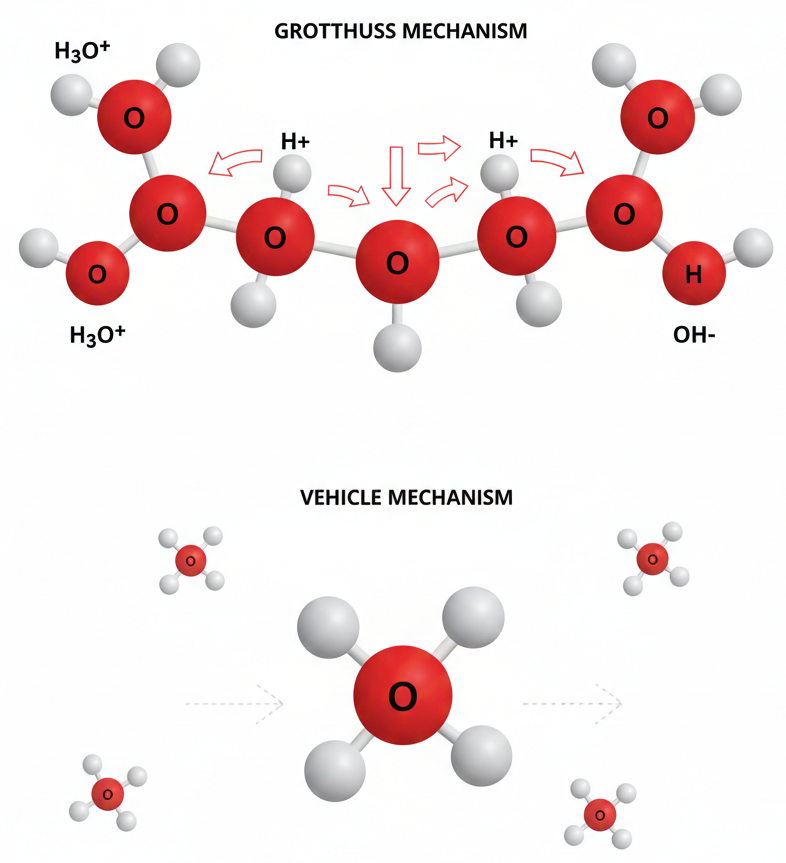
\includegraphics[width=0.5\linewidth]{2.2 grothus and vehicle.png}
\caption{Grotthuss hopping versus vehicular transport mechanisms.}
\label{fig:proton-transport-mechanisms}
\end{figure}

\section{Poly(vinyl alcohol)(PVA):Beyond Commodity Applications}
\subsection{Chemical structure and Functionality}
Poly(vinyl alcohol) has gained considerable interest as a potential base material for alternative membrane materials because of its combination of properties. PVA is industrially produced by the hydrolysis of poly(vinyl acetate), has low production costs compared with fluoropolymers, and its synthesis does not require the use of halogens.\cite{9,10} PVA materials with molecular weights ranging from less than 13,000 to more than 190,000 Daltons are biocompatible and biodegradable and are easily spun into fibrous membrane materials by electrospinning.\cite{10,11}

The PVA repeating unit contains a hydroxyl group, –OH, on every carbon atom of the main chain. These hydroxyl groups engage in extensive intrachain and interchain hydrogen bonding, which is responsible not only for the mechanical toughness of PVA films but also for the possibility of proton transport via these hydrogen bonds. Nevertheless, while the high density of hydroxyl groups makes PVA an interesting material for membrane use, it is also the main cause of PVA’s extreme water solubility, according to Bolto et al., which is considered to be the main hindrance to using PVA in water-based membranes.\cite{29} Designing materials that do not suffer from dissolution while preserving the hydroxyl groups that enable proton transport is considered to be the main engineering problem associated with PVA membranes.

\begin{figure}[h!]
\centering
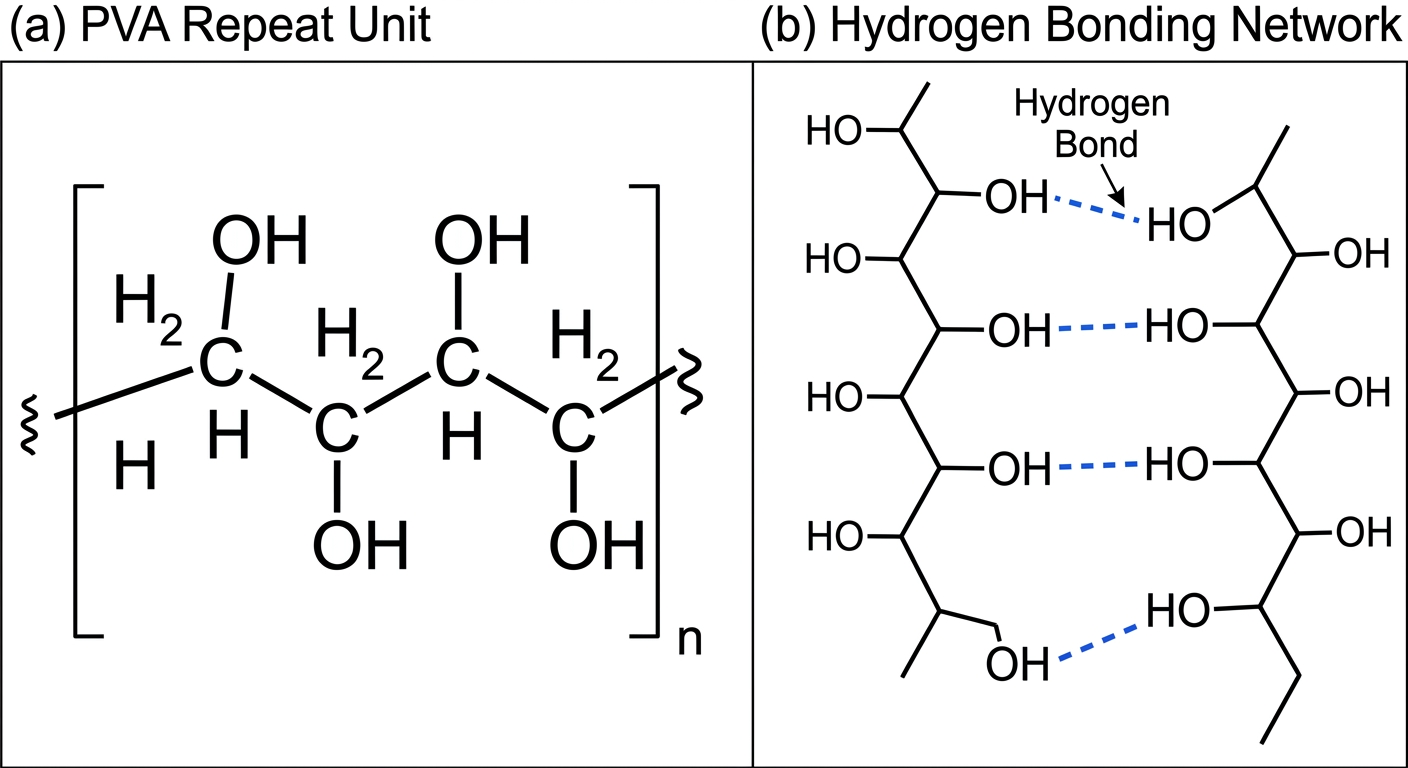
\includegraphics[width=0.8\linewidth]{pva repear unit pendanr oh group.png}
\caption{PVA chemical structure and interchain hydrogen bonding.}
\label{fig:pva-structure}
\end{figure}

\subsection{Semicrystalline Nature of PVA}
PVA has a semicrystalline structure in which crystalline lamellae are present in an amorphous matrix. Hassan and Peppas have shown that the degree of crystallinity and mechanical properties of freeze-thawed PVA hydrogels are a function of the number of freeze-thaw cycles and initial solution concentration, and that crystallinity is due to extensive interchain hydrogen bonding that occurs upon slow cooling.\cite{30} These regions are responsible for providing mechanical integrity to prevent structural collapse under load.

Crystallinity is also a parameter that may be controlled by processing history. Mallapragada and Peppas studied the kinetics of crystallisation in semicrystalline PVA and have shown that previous thermal history has a significant effect on morphology.\cite{31} Ricciardi et al. studied the kinetics of crystallisation from PVA/water solutions and have shown that it is strongly dependent upon polymer concentration, temperature, and chain length.\cite{32} Tretinnikov and Zagorskaya have proposed a method for determining a crystallinity index based upon FTIR spectra by using a ratio of the 1141 cm\(^{-1}\) band due to crystalline material and a 1095 cm\(^{-1}\) band due to amorphous material\cite{33}.

This has significant implications for membrane properties. Crystalline regions are impermeable to both ions and protons, while amorphous regions are permeable. Hence, a compromise between crystallinity and impermeability is a desired state that balances mechanical properties with a degree of impermeability that is still sufficient for proton conduction. This is a significant engineering problem in the construction of PVA membranes.

\subsection{Strategies for Water-Stabilisation}
However, for PVA to perform well in persistent aqueous solutions, the intrinsic water solubility of the polymer has to be significantly lowered. This may be accomplished by physical blending or chemical modification. Physical blending may involve polymer blends and semi-interpenetrating polymer networks. Gohil and Ray discussed the semi-interpenetrating network structure for fuel cell membranes and the impact of blending with other polymers on the water absorption, mechanical properties, and ionic conductivity of the membrane\cite{34}. In all cases, the balance among these properties is improved by the blending with other polymers. Chemical crosslinkeding is more effective in lowering the water solubility of PVA. Jang and Bae studied the thermomechanical properties of crosslinked PVA membranes and showed that a three-dimensional network structure prevents dissolution by inhibiting interchain slipping\cite{35}. Mansur et al. studied the FTIR spectra of PVA hydrogels crosslinked with glutaraldehyde and confirmed the presence of acetal linkages in the network structure. This study thus confirmed the chemistry of crosslinkeding. However, glutaraldehyde is no longer considered a viable crosslinkeding agent because of its toxicity.\cite{36} The study by Rhim et al. established the integrity of PVA films in water and the importance of the crosslinked density not becoming too high and making the membrane brittle.\cite{9}

\begin{figure}[h!]
\centering
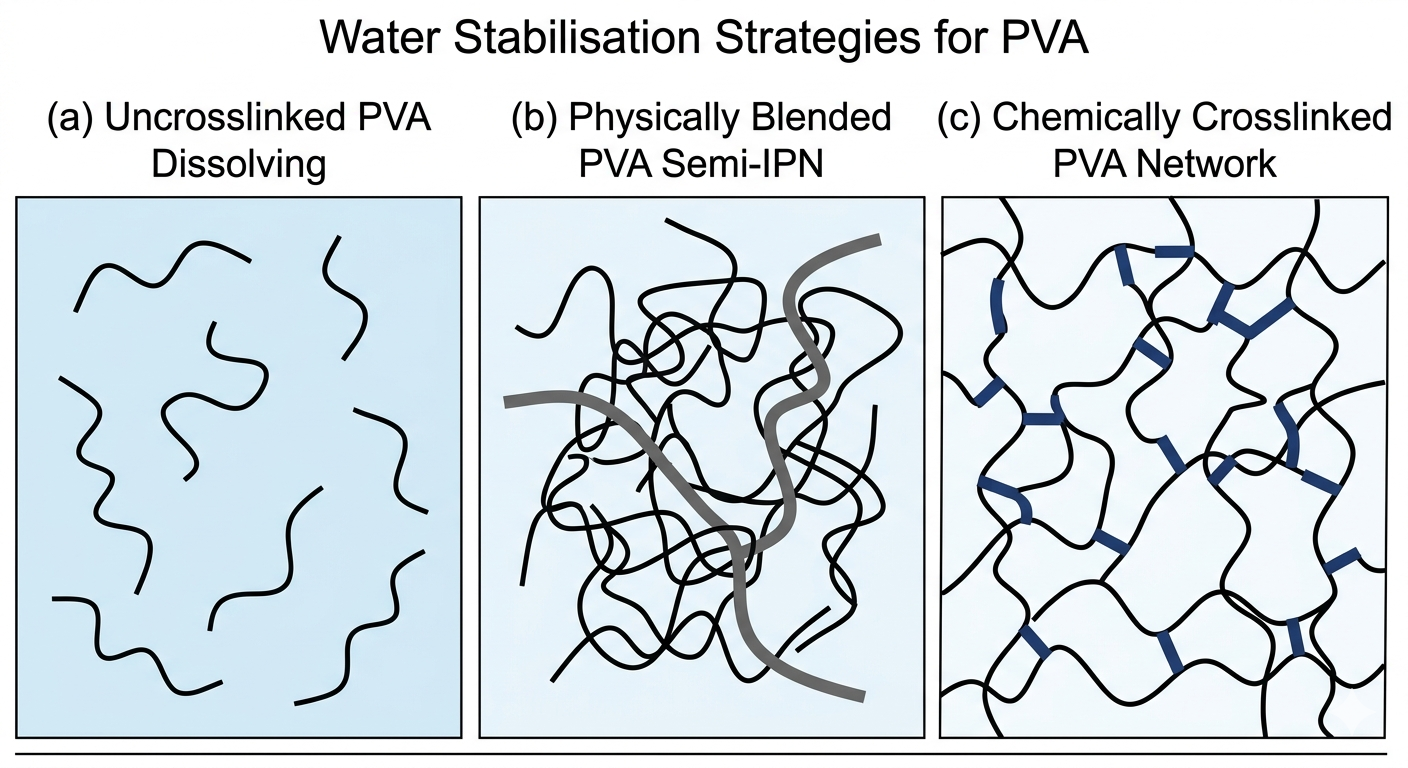
\includegraphics[width=0.8\linewidth]{water stabilization strategies for pva.png}
\caption{Water stabilization strategies for PVA}
\label{fig:pva-stabilisation}
\end{figure}

\section{Advanced Fiber Engineering via Electrospinning}
\subsection{Electrospinning Physics}
This is a versatile method that allows for fibers with diameters ranging from tens of nanometers to a few micrometers in diameter, depending upon the process conditions. Reneker and Yarin have provided a detailed description of the mechanics involved in this process. In this process, a polymer solution is placed in a container with a positively charged tip. When the electrostatic force becomes greater than the surface tension, a cone-like shape is produced, called the Taylor cone\cite{37}. A jet of solution emerges from the tip of this cone and follows a random path as it dries quickly and becomes thinner. Greiner and Wendorff have emphasized that this process is advantageous in producing ultrafine fibers that have unique structural and functional properties, and that this process allows for aligned molecular chains that have a significant effect on mechanical and transport properties\cite{38}.

In a study on the bending instability of electrospun jets, Luo et al. concluded that the chaotic whipping motion of the fiber in flight primarily determines the final fiber morphology. This is the reason why the process conditions need to be precisely controlled in order to achieve the desired fiber size, as well as the fiber diameter distribution, as the voltage, solution feeding rate, distance between the tip and collector, as well as the properties of the solution, influence the final product\cite{39}.

\begin{figure}[h!]
\centering
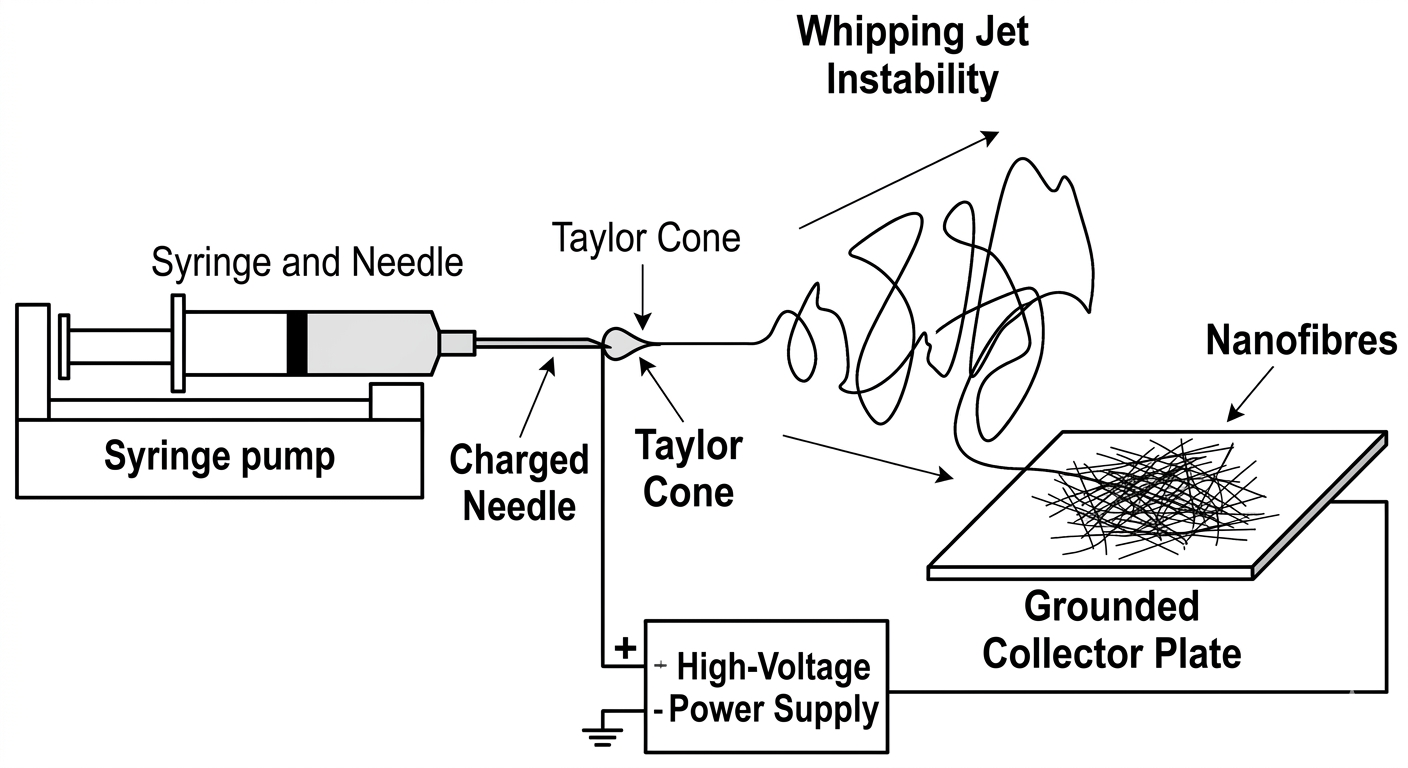
\includegraphics[width=0.8\linewidth]{electrospinning.png}
\caption{Schematic of the electrospinning process.}
\label{fig:electrospinning Syringe machine}
\end{figure}

\subsection{Nanofiber vs. Bulk Film}
Electrospun nanofiber mats offer distinct advantages in terms of ion transport properties in comparison to the conventional dense films obtained through the casting process. The interesting feature of the nanostructure is the large surface area to volume ratio, thus providing a large number of interfacial sites for proton exchange. In their investigations on the electrospun fibres of Nafion, Chen et al. reported an increase in conductivity in comparison to the cast films, but only at specific humidity levels. They attributed the increase in conductivity to the favorable orientation of the chains, a feature of the electrospinning process\cite{40}. Another interesting feature reported in the investigations by Dong and co-workers is the directional character of the proton conduction in the aligned nanofibers embedded with Nafion. They reported the collection of the fibres in a particular orientation while spinning the fibres and thus enabled the through-plane proton conduction\cite{41}.

Aligned nanofiber networks, according to Tamura and Kawakami, provide shorter paths for proton transport, unlike the meandering routes required in dense films, where lower tortuosity greatly enhances conductivity.\cite{42} Proton transport is improved in electrospun nanofiber membranes, according to Choi et al., whose improvements were due to a combination of high surface area, low crystallinity compared to bulk films, and continuous proton transport routes on the surface of fibers following the addition of acid group functionalization.\cite{43}

\begin{figure}[h!]
\centering
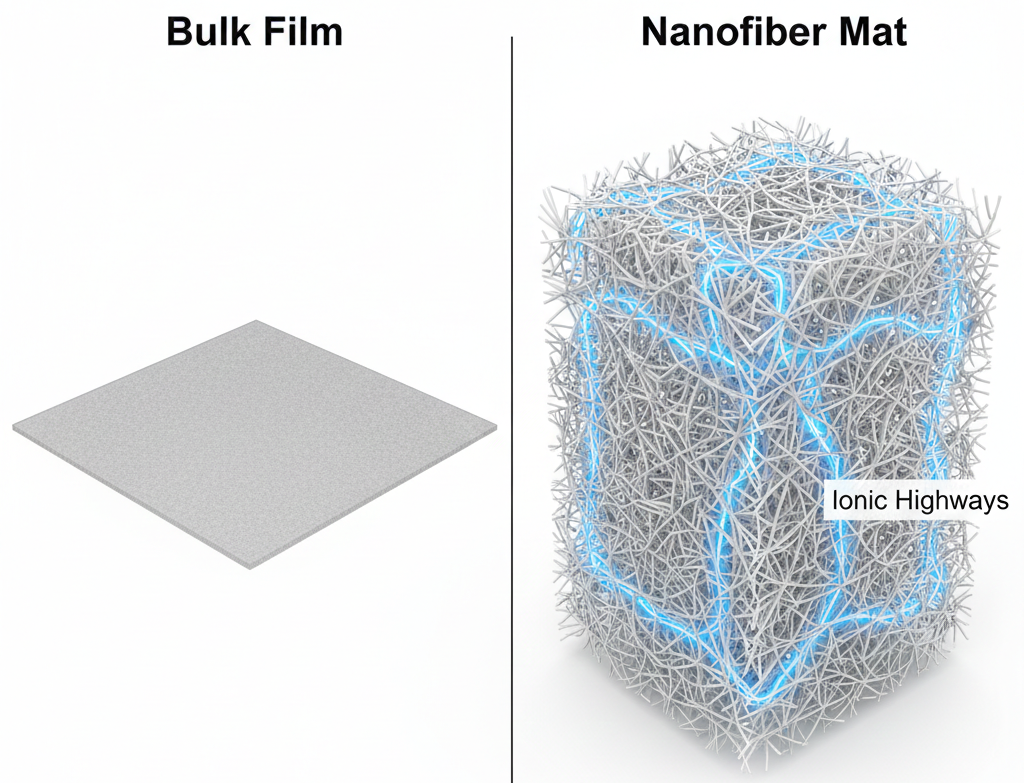
\includegraphics[width=0.5\linewidth]{4.2 nano fiber vs bulk.png}
\caption{NanoFibrous mat vs Film}
\label{fig:nanofiber-vs-film}
\end{figure}

\subsection{Rheological Prerequisites}
The quality of electrospun fibers is determined by the viscoelastic characteristics of the initial solution. Shenoy, et al. have studied the importance of chain entanglement in electrospinning, revealing that there is a need to have a certain level of entanglement density to provide the elastic restoring force, which prevents the jet from breaking up into droplets and instead creates continuous fibers.\cite{44} McKee, et al. have quantified this, revealing that the entanglement number needs to exceed a threshold of 2.5 to form fibers. If this is not exceeded, then entanglement is not enough to create a continuous jet, while if it is exceeded, then fiber diameters increase with viscosity.\cite{45}

In a study, Palangetic et al. discussed the PVA blend’s performance in terms of steady and fluctuating flows during the electrospinning process, with the main point being that the right balance of concentration and shear rate is important in order to keep the fluid intact during the spinning process.\cite{46} Bapna et al. studied the spinning window and the shape of the fibres for PVA/citric acid solution, identifying the concentration range that enables the production of defect-free fibres, with the addition of citric acid influencing the acidity as well as the viscosity of the solution.\cite{47}

\section{Green Crosslinking Chemistry:The Polycarboxylic Acid Route}
\subsection{Esterification Kinetics}
Polycarboxylic acids are non-toxic crosslinkers for PVA and form crosslinks by esterifying the –OH groups of PVA. Gohil and Ray’s studies demonstrated the crosslinking of PVA with carboxylic acids and the formation of a stronger network with improved water resistance. The crosslinking is non-toxic and does not leave behind residues.\cite{48} The dehydration of the –OH group of PVA and the –COOH group of the crosslinker is the major step in the esterification. Ester bond formation in PVA and starch film crosslinked with citric acid was studied by Shi et al. and verified by infrared spectroscopy.\cite{49} The temperature has a significant impact on the esterification reaction. Increasing the temperature accelerates the esterification reaction; however, increasing the temperature beyond the PVA degradation temperature causes degradation of the polymer chain. Kinetic models for the crosslinking of PVA with polycarboxylic acids by Uranga and colleagues demonstrated the second-order dependence of the crosslinking kinetics on the concentration of the –OH and –COOH groups. The presence of more than one –COOH group in the crosslinker allows the crosslinker to crosslink more than one polymer chain and form a network.\cite{50} The crosslinking of PVA with polycarboxylic acids can be monitored by FTIR. The decrease in the absorption band around 3300 cm\(^{-1}\) corresponding to the –OH group and the increase in the absorption band around 1730 cm\(^{-1}\) corresponding to the ester carbonyl group can be monitored by FTIR.\cite{36,53}

\subsection{Multi-functional Crosslinkers}
The number of reactive groups in a molecule of a crosslinkeder plays a significant role in determining the final network structure. For example, citric acid has three carboxyl groups and one hydroxyl group. This results in the ability of citric acid to create a network of densely interconnected molecules. In a recent study by Birck and colleagues, the changes in the structure of PVA membranes with increasing amounts of citric acid were studied. The results showed that with moderate amounts of a crosslinkeder, water resistance and stiffer membranes are obtained. However, the material becomes brittle with excessive amounts of the crosslinkeder, as the mobility of the chains is restricted beyond what is necessary for dimensional stability. \cite{51}
In a separate study by Sood and colleagues, the properties of membranes for proton exchange were studied. The results showed that the location of the crosslinkeds in the membrane plays an important role in maintaining the integrity of the material. A heterogeneous distribution of crosslinkeds results in a reduction in the material’s performance.\cite{52}

\subsection{Thermal Activation}
However, it’s not possible to crosslink PVA with polycarboxylic acids at room temperature; it requires a heat start. Gohil and Ray have shown that it’s necessary to be around 130-160 degrees Celsius in order to get this process off without breaking the main polymer chain.\cite{34} However, Birck and coworkers have shown that it’s also important to avoid dehydration reactions that occur when the process is prolonged or the temperature is high; this leads to the formation of conjugated polyenes and a resulting yellow color and decrease in mechanical and transport properties.\cite{51} Parida and coworkers have studied the kinetics of heating PVA in citric acid and have shown that it’s necessary to be at 150 degrees Celsius for 60 minutes in order to get a good balance between crosslink density and avoiding thermal degradation.\cite{53} However, it’s important to control the temperature precisely in order to get a repeatable crosslink density in electrospun membranes made from a mixture of PVA and citric acid, as shown by Wang and coworkers.\cite{54}

\section{Acid based doping and Membrane Functionalization}
\subsection{Phosphoric Acid (H\(_3\)PO\(_4\)) as a Liquid Electrolyte}
Among the proton conducting dopants for polymer electrolyte membrane materials, phosphoric acid is one of the most potent and has been extensively investigated as a pure compound and as a dopant. In a study by Vilciauskas et al., the proton transport mechanism for the pure compound was investigated. The study showed a combination of structural diffusion and vehicular processes for the proton.\cite{21} The high proton conductivity of the compound compared to other liquid electrolytes is attributed to the high density of hydrogen bonds and the high intrinsic mobility of the phosphate species. The compound is thus effective even without the presence of liquid water and at temperatures above 100\(^\circ\)C.\cite{55}

The reviews on phosphoric acid-doped membranes for high-temperature fuel cells show that the use of H\(_3\)PO\(_4\) as a dopant enables the fuel cell to operate above 120\(^\circ\)C without the need for humidification. This greatly simplifies the system, as it avoids the need to include a system to provide humidity to the fuel cell as required by PFSA membranes.\cite{56,57} Wang et al. reviewed phosphoric acid-doped polybenzimidazole (PBI) membranes, which have been the most researched in this area to date, to the point where they have become available commercially. However, due to their high cost and difficulty of processing, there remains interest in other polymers that can effectively retain phosphoric acid.\cite{58}

\begin{figure}[h!]
\centering
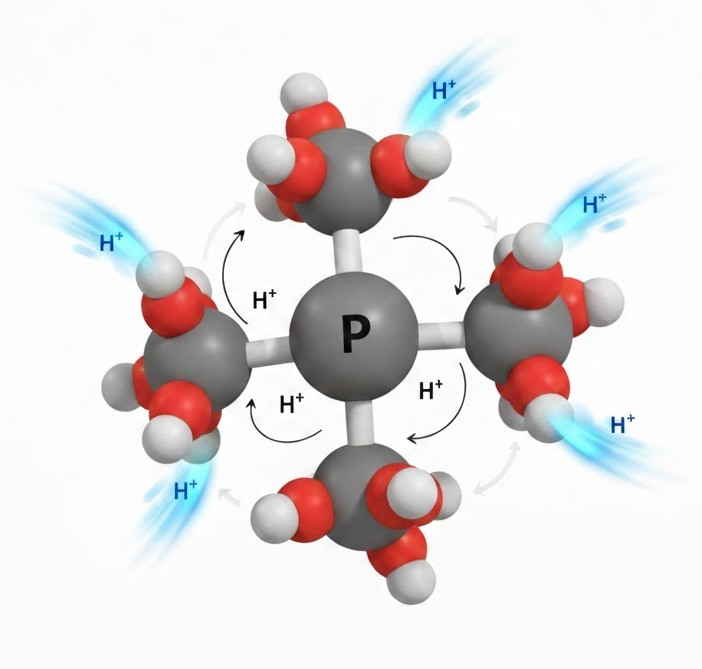
\includegraphics[width=0.5\linewidth]{proton hopping mechanism.jpg}
\caption{Proton Hopping mechanism}
\label{fig:Proton Hopping}
\end{figure}

\subsection{Acid-Polymer Interactions}
The manner in which the phosphoric acid interacts with the host polymer matrix is the main determinant of the behavior of the final membrane in use. In studies carried out by Sood et al., FTIR and NMR spectroscopy were used in the examination of molecular interactions in acid-doped polymer films, showing that hydrogen bonding occurs easily between the phosphoric acid and the –OH groups of the polymer film, with the bonding being strong enough to retain a significant amount of the acid in the polymer matrix, preventing the complete leaching out of the acid in the material upon washing with water.\cite{52} Jang and Bae studied the retention of acid in crosslinked electrolytes for use in high-temperature applications, showing that the process of crosslinking the materials acts as a deterrent against swelling, thus aiding in the retention of the acid, though the process of crosslinking detracts from the free volume in the material as well as the lengths of the proton transport pathways.\cite{35}

Scientists like He and their team have examined the mobility of protons and the binding of acids with functional groups in phosphoric acid-doped polybenzimidazole membranes. They measured the binding energy between the acid and the polymer sites. They created a reference guide to compare the binding of acids in different polymers.\cite{59} In the same vein, Nomura and their team have examined the hydrogen bonding between the polymers and the acids in PVA/citric acid membranes. They found an optimal binding energy. Binding energy that is too low or too high is not optimal. Excessive binding causes the acids to be immobile.\cite{60}


\begin{figure}[h!]
\centering
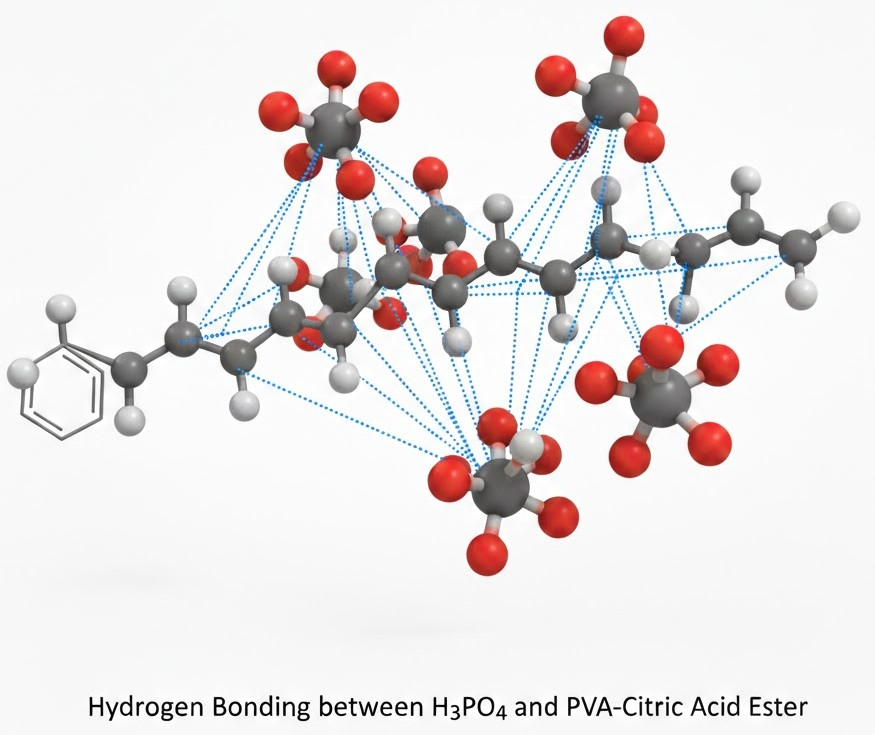
\includegraphics[width=0.5\linewidth]{hydrogen bond bw h3po4 and pva ca.jpg}
\caption{Hydrogen bond between H3PO4 and Esterified PVA}
\label{fig:Hydrogen bond}
\end{figure}

\subsection{The Plasticisation Effect of Phosphoric Acid}
Phosphoric acid has a twofold effect in that it reduces the glass transition temperature by plasticising the host polymer matrix and acts as a proton carrier. With increased levels of phosphoric acid, the polymer becomes more mobile, which allows the protons to move around more easily, but it also becomes softer and compromises its mechanical properties under compressive load.\cite{4} The process of crosslinking offsets this by maintaining mechanical integrity in the polymer matrix even as it becomes more mobile. This is why citric acid crosslinking is carried out before phosphoric acid doping in our process and not simultaneously.\cite{35,53} The main reasons for degradation in phosphoric acid-doped membranes, as identified by Wang and coworkers, are plasticisation-induced softening, acid leaching, and degradation of crosslinks due to hydrolysis.\cite{58}

\section{Computational Modeling of Proton Exchange Membranes}
\subsection{Density Functional Theory in Membrane Science}
While experimental characterisation indicates what a membrane does in a given situation, DFT analysis indicates why it does this in this way. The transfer of protons occurs in femtoseconds and over angstroms, scales that are beyond any measurement capability for macroscopic properties. However, DFT is designed to operate at this scale. Measurement of conductivity indicates that proton transfer does occur, and DFT analysis indicates the route by which this occurs, the energy barrier for the process, and the way in which the electronic structure is altered as bonds break and reform. This complementary relationship has ensured that DFT is an accepted method in membrane studies, often in conjunction with experimental characterisation in studies aimed at a molecular-level understanding.\cite{18,19}

\subsection{Published DFT Studies: Nafion, SPEEK, and PBI–H\(_3\)PO\(_4\)}
The system that has been studied more extensively than any other in the field of membrane science is Nafion. Paddison and colleagues have performed a series of ab initio studies that demonstrated the activation energy required for the dissociation of a proton from a sulfonic acid group decreases with increasing levels of hydration. This provided the first quantum description of the influence of water content on the conductivity of Nafion.\cite{18,19}
Another material that has been extensively investigated with DFT is polybenzimidazole doped with phosphoric acid. In the study of PBI/H\(_3\)PO\(_4\) clusters, the binding energy, the structure of the hydrogen bonds, and the proton transfer barriers were all determined to lie in the range of 20–50 kJ/mol.\cite{20,59} Perhaps more important, however, the DFT-calculated barriers were shown to be comparable to the experimentally determined activation energies by an Arrhenius fit of the data. In the study of PBI/H\(_3\)PO\(_4\) clusters, the changes in bond orders along the proton transfer path have been investigated by calculating the natural bond orbital changes. The paths by which the protons are transported, as electron-poor pathways, have been visualized by the use of the electron localization function. The methodology used is discussed in the next chapter.

\subsection{Molecular Dynamics Simulations of Proton Transport}
Molecular dynamics is a complementary tool to static DFT, which allows us to catch a glimpse of the dynamic, concerted side of proton transport, which is not accessible using cluster-based DFT. The pioneering work by Tuckerman, Marx, and Parrinello using ab initio MD provided the first atomistic, real-time view of the Grotthuss mechanism in water, revealing that proton transport is not simply the diffusion of a hydronium ion, but rather a concerted process that involves the rearrangement of the hydrogen bond network.\cite{61,62} In their study, they were also one of the first to propose the concept of a "proton wire," defined by a chain of hydrogen bonds through which protons move collectively, a concept that is now commonplace in discussions of mechanisms in membranes.

Subsequent classical and coarse-grained MD studies have developed this concept for Nafion-type membranes. This work indicated that the transport through the sulfonic acid groups is a combination of Grotthuss and vehicular transport, with the proportion of the two depending on the water content and the inner domain structure.\cite{63} Kreuer summarized the NMR, conductivity, and simulation data for several membrane systems to propose a key concept. This concept is as follows: the most promising membrane is that in which Grotthuss transport is possible even at low hydration levels. This is relevant to the phosphoric acid-doped system studied in this dissertation.\cite{64}


\subsection{Molecular Dynamics Simulations of Proton Transport in PEMs}

Classical molecular dynamics simulation has become an indispensable 
tool in Proton Exchange Membrane research, offering access to structural 
and transport properties that neither experiment nor DFT can provide 
alone. Where DFT captures the quantum mechanics of individual bond 
formation and proton transfer, MD propagates the motion of thousands 
of atoms over nanosecond timescales, revealing how molecular-scale 
interactions manifest as macroscopic transport behaviour such as water 
uptake, acid retention, and proton diffusion \cite{64}.

The most extensively studied membrane by MD is Nafion. Venkatnathan 
et al.\ (2007) demonstrated that water cluster connectivity in Nafion 
controls the crossover from vehicular to Grotthuss-dominated proton 
transport, identifying a structural percolation threshold at 
approximately fifteen water molecules per sulfonate group. Their 
radial distribution functions between sulfur and water oxygen atoms 
shifted systematically with hydration level, providing a direct 
structural fingerprint of swelling behaviour. Devanathan et al.\ 
(2007) extended this picture by showing that the nanophase-separated 
morphology of Nafion emerges naturally from MD trajectories without 
any imposed structural assumptions, and that the connectivity of 
hydrophilic domains — not their total volume — governs conductivity.

For PVA-based systems, MD has been used to quantify how crosslink 
density affects chain mobility and water transport. Zhao et al.\ 
(2016) showed that citric acid crosslinking suppresses swelling by 
restricting chain segment motion, while preserving the hydrophilic 
hydroxyl channels that carry protons. Their simulations confirmed that 
the crosslink density optimum lies at a stoichiometry that balances 
dimensional stability against conductivity — exactly the trade-off 
explored experimentally in the present work. The OPLS-AA force field, 
used in all of these studies, has been validated exhaustively for 
organic systems containing hydroxyl, ester, carbonyl, and phosphate 
groups \cite{95}, making it the natural choice for the 
PVA/CA/H\(_3\)PO\(_4\) system studied here.

\subsection{Finite Element Analysis for Fuel Cell Performance 
Prediction}

Finite element analysis translates membrane transport properties 
measured at the molecular or experimental scale into device-level 
performance predictions. The foundational framework was established 
by Springer et al.\ (1991), who modelled the polymer electrolyte 
membrane as a homogeneous medium characterised by a single 
experimentally determined proton conductivity, and solved the 
conservation equations for ionic current, water activity, and 
electrochemical potential across a full membrane electrode assembly. 
Berning and Djilali (2003) extended this to a full three-dimensional, 
multiphase model incorporating gas diffusion layer transport, catalyst 
layer kinetics governed by the Butler--Volmer equation, and ohmic 
losses in the membrane domain. Their work established the now-standard 
COMSOL implementation used in single-cell PEMFC studies.

The central governing equation in the membrane domain is the 
conservation of ionic current:

\begin{equation}
\nabla \cdot \left( \sigma_{m} \nabla \phi_{m} \right) = 0
\end{equation}

where \(\sigma_{m}\) is the proton conductivity of the membrane 
(S\,cm\(^{-1}\)) and \(\phi_{m}\) is the ionic potential (V). 
Electrochemical kinetics at the electrode interfaces are described 
by the Butler--Volmer equation \cite{66}:

\begin{equation}
i = i_0 \left[ 
\exp\!\left(\frac{\alpha_a F \eta}{RT}\right) - 
\exp\!\left(-\frac{\alpha_c F \eta}{RT}\right) 
\right]
\end{equation}

The power of this framework lies in its direct connection to 
experiment: the proton conductivity \(\sigma_{m}\) measured by EIS 
is inserted unchanged into the FEA model, propagating real material 
properties to the polarisation curve. Siegel et al.\ (2003) 
demonstrated this workflow for a sulfonated polymer membrane, 
obtaining polarisation curves in quantitative agreement with 
experiment using only EIS-measured conductivity and SEM-measured 
membrane thickness as inputs. This is precisely the approach adopted 
in the present work for the PVA/CA/H\(_3\)PO\(_4\) system.

\subsection{The Computational Gap: PVA/CA/H\(_3\)PO\(_4\)}

In spite of the extensive computational studies of Nafion, 
sulfonated aromatic polymers, and PBI, the 
PVA/CA/H\(_3\)PO\(_4\) system has never been investigated 
using DFT, classical MD, or finite element approaches. This 
is significant because the proton exchange environment of 
this system is chemically unique compared with all previously 
studied membranes. The hydrogen-bond network consists of 
PVA hydroxyl groups, ester bonds formed by thermal 
crosslinking, and the multiple donor-acceptor sites provided 
by H\(_3\)PO\(_4\) molecules.\cite{20,59}

The specific questions that remain unanswered at a molecular 
level include how multiple acid molecules interact 
cooperatively when binding to neighbouring hydroxyl groups, 
how ester crosslinks affect proton hopping barriers, the 
thermodynamic stability of the acid-polymer-water ternary 
complex, and the energy landscape for proton transfer. 
Beyond this, no study has applied classical MD simulation 
to characterise acid retention dynamics or swelling in this 
system, and no finite element model exists to translate its 
transport properties to device-level polarisation 
behaviour.\cite{53,54}

A further question untouched by any previous computational 
work is whether replacing the hydrogen bond between 
phosphoric acid and PVA with a covalent P--O--C linkage 
would eliminate acid leaching without reducing proton donor 
activity. This dissertation addresses all of these research gap 
through a three-tier multiscale framework combining DFT, 
classical MD, and finite element analysis, and includes 
the first computational comparison of hydrogen-bonded and 
covalent phosphate binding modes in a PVA membrane 
system.\cite{18,19}



\section{Characterization Techniques in Membrane Science}
\subsection{Spectroscopic Analysis (FTIR)}
Fourier Transform Infrared Spectroscopy is a highly effective method to explore polymer membranes at the molecular level. In one such study, Mansur et al. utilized FTIR spectroscopy to monitor esterification reactions in PVA-based polymer networks, where the broad O–H stretch band around 3300 cm\(^{-1}\) disappears as hydroxyl groups react, while a new band due to C=O stretches around 1730 cm\(^{-1}\) emerges to signal esterification. Another method to utilize FTIR spectroscopy is to develop methods to analyze FTIR spectra to determine crosslink density in polymer electrolytes by comparing the area of ester carbonyl bands with a reference band, enabling optimization of esterification reactions.\cite{52}

Yet another level of structural understanding is provided by solid-state NMR spectroscopy. In acid-doped polymer membranes, for example, \(^{13}\)C NMR spectroscopy that specifically detects different carbon environments verifies the existence of ester linkages, and \(^{31}\)P NMR spectroscopy provides evidence for the chemical form of the incorporated phosphoric acid.\cite{52,59} A more quantitative understanding is provided by pulsed-field gradient NMR spectroscopy, which allows for the measurement of proton self-diffusion coefficients in crosslinked PVA-phosphoric acid systems.\cite{60}

\subsection{Structural Analysis (XRD and SEM)}
X-ray diffraction is a technique for measuring the level of crystallinity of a polymer membrane. For example, Tretinnikov and Zagorskaya employed X-ray diffraction as a tool for characterizing phase transitions in crosslinked PVA membranes. They identified the major peaks at 2\(\theta\) = 19.5\(^\circ\) and 40.5\(^\circ\), which are associated with the semicrystalline structure of PVA, and demonstrated that variations in peak intensities correlate well with changes in crystallinity induced by crosslinking or acid doping. \cite{33} Mallapragada and Peppas investigated the influence of varying amounts of crosslinking agents on the level of crystallinity of PVA membranes. They demonstrated that an increase in the level of the crosslinking agent steadily decreases the level of crystallinity, which is consistent with the influence of covalent crosslinking on the regularity of polymer chains.\cite{31}

Scanning electron microscopy provides a "direct view" of membrane morphology. In their study, Luo et al. emphasized the advantage of high-resolution visualization, specifically of electrospun nanofibers, where SEM is utilized to "characterize the size distribution, surface texture, and defects such as beading or welding of fibers.\cite{39}" Jang and Bae utilized SEM to study changes in nanofibrous mats, specifically how these mats change shape upon heat treatment and acid exposure, where "heating causes fibers to become tightened and smoother, while acid causes swelling and fusion of fibers," which is related to changes in morphology discussed in Chapter 4 of this dissertation.\cite{35}

\subsection{Electrochemical Impedance Spectroscopy}
Electrochemical impedance spectroscopy continues to be the preferred method of measurement of ionic conductivity of polymer electrolyte membranes. Macdonald presented the theory of impedance spectroscopy,\cite{65} while Orazem and Tribollet presented the practical approach.\cite{66,67}
For a typical electrochemical impedance spectroscopy analysis, you subject your membrane to a small oscillating voltage and monitor how the current responds as you vary the voltage’s frequency. The resulting data is often presented in two forms: a Nyquist plot, in which the imaginary component is plotted against the real component, and a Bode plot, in which the real and imaginary components are plotted against the frequency. When working with ion-conducting membranes, it’s worth noting that the high-frequency intercept on the real axis in a Nyquist plot will yield the bulk resistance of your membrane and allow you to calculate your membrane’s proton conductivity. In one study, Sood and coworkers used EIS to study nanofibrous Proton Exchange Membranes and examine how membrane structure influences ohmic resistance.\cite{52} In another study, Nomura and coworkers used temperature-dependent impedance measurements to study acid-doped PVA/citric acid membranes and examine how membrane structure influences proton transport by determining activation energy values.\cite{60}

\section{Research Gap and Scope}
Despite significant progress in alternative Proton Exchange Membranes (PEMs), several research gaps remain. While Poly(vinyl alcohol) (PVA) is a well-studied material, most literature focuses on its use in water filtration rather than energy conversion \cite{11}. Furthermore, while phosphoric acid ($H_3PO_4$) doping is common for high-temperature polymers like PBI \cite{20,59}, there is very little research on its application in electrospun PVA nanofibers. Most studies on PVA-citric acid crosslinking are restricted to dense cast films, missing the potential benefits that the high surface area of nanofibers could offer for proton transport \cite{53,54,68}.

A major practical challenge that has not been fully explored is the trade-off between acid uptake and mechanical stability. Specifically, doped polymer electrolytes face a persistent problem with acid leaching during hydration \cite{35}. There is a clear need for a quantitative, molecular-level understanding of these degradation processes \cite{58}. Until now, no study has applied a comprehensive computational framework to this specific system to characterize the thermodynamics of acid binding, the exact mechanism of proton hopping, or the chemistry of acid retention. 

This research bridges these gaps by combining experimental fabrication with a hierarchical computational approach. We fabricated PVA/CA membranes via electrospinning and systematically doped them at three time intervals (30 min, 2 h, and 24 h). To investigate the molecular origins of performance, we performed 31 sets of DFT calculations (B3LYP-D3BJ/6-31G*) to map the transition from hydrogen-bonded doping to a more stable covalent $P-O-C$ linkage. These findings were validated at operating temperatures ($353.15$ K) using molecular dynamics in LAMMPS to confirm structural stability. Finally, we utilized Finite Element Analysis in COMSOL to translate these atomistic results into a macroscopic device model. This multiscale framework allows us to describe the $PVA/CA/H_3PO_4$ system for the first time across all scales—from a single chemical bond to the performance of a functioning fuel cell \cite{21,79}.


\chapter{Methodology (Experimental and Computational)}

The experimental approach for the synthesis of electrospun poly(vinyl alcohol) nanofiber membranes is discussed in detail in this chapter. These membranes are crosslinked with citric acid and doped with phosphoric acid. All experiments were conducted at the Department of Physical Chemistry, National University of Science and Technology MISIS (NUST MISIS), Russia. Furthermore, the computational approach for the entire density functional theory calculations is discussed.

\section{Materials and reagents}
\subsection{Polymer matrix:}
The major constituent polymer in the membranes is poly(vinyl alcohol) (PVA), a widely used polymer with many applications. The PVA used in this work is supplied by RusKhim Company in Moscow, Russia. The molecular weight is in the range of 80,000-124,000 Da, and the hydrolysis degree is in the range of 88-97\%. This grade of PVA is chosen for its ability to be electrospun and for its good balance of water solubility\cite{10,11} for easy handling and film-forming ability.\cite{44,45} The PVA is used as received without further purification and is dried in a desiccator at room temperature.

\subsection{Citric Acid}
The anhydrous citric acid used in this study has a molecular weight M\(_w\) of 192.12 g/mol and a purity of more than 99.5\%, and it was obtained from Mirfouds in Russia. The trifunctional carboxylic acid structure of citric acid enables it to react with the hydroxyl groups of PVA to form multiple ester bonds and a three-dimensional crosslinking structure.\cite{50,51} In contrast to other crosslinkers such as glutaraldehyde, citric acid is non-toxic and biodegradable and is permitted for use in food contact applications, which aligns with the principles of green chemistry.\cite{48, 53}

\subsection{Phosphoric acid}
The orthophosphoric acid, with a concentration of 85 wt\% in water and a purity of more than 99\%, was donated by the Physical Chemistry Department of NUST, MISIS. Phosphoric acid was selected for the study owing to its exceptional proton conductivity, high thermal stability, and capability for acting as a proton acceptor and donor in both hydrated and dry forms.\cite{55,56} The amphoteric property of H\(_3\)PO\(_4\) is also useful for Grotthuss-type hopping.\cite{21}

\subsection{Solvent system}
The only solvent used for the preparation of solutions was deionised water with a resistivity of more than 18.2 M\(\Omega\cdot\)cm, obtained from NUST MISIS. The use of water as a solvent also removes the use of toxic organic solvents, thus emphasizing the eco-friendliness of the fabrication method.\cite{54} Water also helps as a plasticiser during electrospinning, allowing the polymer chains to move more easily.\cite{46}

\section{Preparation and Rheological}
\subsection{Solution Stoichiometry}
The precursor solutions were carefully formulated with specific weight fractions to ensure optimal electrospinning and crosslinkeding. The primary solution is composed of 9 wt\% PVA and 10 wt\% citric acid with reference to the weight of the PVA. This is a result of earlier optimization and established literature for PVA-CA combinations. \cite{46,47}

To create a typical 50 g precursor solution, 4.5 g of PVA powder is accurately measured with a VIBRA AJ-220CE analytical balance (Shinko Denshi Co., Ltd., Japan), with a tolerance of \(\pm\)0.0001 g (Figure 3.1). This is followed by the incorporation of 0.45 g of citric acid, equivalent to 10 wt\% of the PVA mass. The remaining 45.05 g is deionized water. This results in a mass fraction of solids to solvent of 1:9, which is within the optimal range for the electrospinning of aqueous PVA solutions, as reported by Palangetic et al.\cite{46}



\subsection{Dissolution Kinetics}
The dissolution was carried out by employing a BIOSAN MSH300 magnetic stirrer with a heat source, as depicted in Figure 3.2.

Steps:
\begin{itemize}
    \item Initial Hydration: Heat the deionized water at 60\(^\circ\)C in a 100 mL borosilicate glass beaker. Slowly add the PVA powder by stirring the solution at 300 rpm for 10 minutes.
    \item Dissolution: Increase the temperature of the solution to 90\(^\circ\)C and maintain it for 3 hours. Stir the solution at 500 rpm. Increasing the temperature facilitates the breaking of the interchain hydrogen bonds in the PVA polymer chain. This allows the polymer chain to dissolve completely. \cite{30,32}
    \item Addition of Crosslinker: Once the PVA is completely dissolved and the solution is clear, decrease the temperature of the solution to 60\(^\circ\)C. Then, citric acid is added to the solution and stirring is continued for another 30 minutes.
    \item Degassing: The solution is cooled to room temperature (25\(^\circ\)C).\cite{39}
\end{itemize}



\subsection{Optimisation of Concentration}
In order to determine the exact amount of PVA required for the solution, a side-by-side test was conducted. Two solutions were created: one with 7 wt\% PVA and the other with 9 wt\% PVA. Then the solutions were tested for the electrospinning capability. For the solution with 7 wt\% PVA, the polymer chains did not entangle enough for the solution to reach the critical overlap concentration. This caused the solution to have the tendency for electrospraying. This phenomenon is in accordance with the theory proposed by Shenoy et al.\cite{44} and McKee et al.\cite{45} The number of entanglements for the solution with 7 wt\% PVA was estimated to be less than 2.5. This number is not enough for the solution to be electrospun.

On the other hand, the solution with 9 wt\% PVA had enough entanglements for the solution to be electrospun. The number of entanglements for this solution was estimated to be around 3.2. In order to validate this result, a dynamic viscosity test with the use of the NUST MISIS device was conducted. For the solution with 9 wt\% PVA and CA, the dynamic viscosity was around 850 cP. This falls within the electrospinning window of 500-2000 cP.\cite{46,47}

\section{Nanofabrication via Needle-Based Electrospinning}
\subsection{Electrospinning Instrumentation}
A customized needle-based electrospinning setup from NUST MISIS was used for the fabrication of the nanofiber membranes. The components used are as follows:
- High voltage source: A PLAZON DC supply unit from Russia, which can be set from 0-50 kV with a current limit of 0.5 mA. The unit supplies the electrostatic voltage required for the fabrication of nanofibers, with a voltage display accurate to \(\pm\)0.1 kV.
- Syringe pump: A LEGATO 100 single syringe pump, which is used for the accurate delivery of the polymer solution. The pump can deliver a range of flow rates from 0.001 \(\mu\)L/hr to 220.8 mL/hr with an accuracy of \(\pm\)0.5\%.
- Spinneret: The polymer solution is placed in a disposable BD Luer Lok syringe with a capacity of 10 mL. The blunt tip stainless steel needle used in the setup has an inner diameter of 0.514 mm, a length of 25 mm, and is used with the positive voltage supply through an alligator clip.
- Collector: The collector used in the process is a sheet of 99.5\% pure aluminum foil with a thickness of 0.1 mm, placed on a grounded stainless steel plate measuring 150 mm x 150 mm.

\subsection{Parameter Control}
The electrospinning parameters were further improved through a combination of initial tests and literature studies for PVA solutions. The final parameters were:
\begin{enumerate}
    \item Voltage: 22 kV, polarity: positive
    \item Tip-collector distance: 18 cm
    \item  Flow rate: 0.5 mL/hr
    \item Spinning time: 1-1.5 hours
\end{enumerate}

The 22 kV voltage was chosen because it is higher than that required to form a Taylor cone, while not causing a corona discharge. A tip-collector distance of 18 cm was chosen because it is sufficiently high to allow time for solvent evaporation before the jet reaches the collector, thus preventing wet fibers, while still being high enough to provide a strong enough electric field to draw out a jet.

\subsection{Environment Monitoring}
Environmental parameters during electrospinning were closely monitored, as these parameters affect the morphology of electrospun fibers:
- Temperature: This was set to 25 \(\pm\) 2 \(^\circ\)C using climate control available in our laboratory. Temperature was monitored every 5 minutes.
- Relative humidity: This was set between 45\% and 55\% RH using a humidifier/dehumidifier combination. This range is appropriate for the water-based solvent system, as lower humidity causes evaporation to occur too quickly, potentially leading to premature jet solidification, while higher humidity causes drying to occur too slowly, potentially leading to wet fibers with adhesion between them.\cite{38,39}

\begin{figure}[h!]
\centering
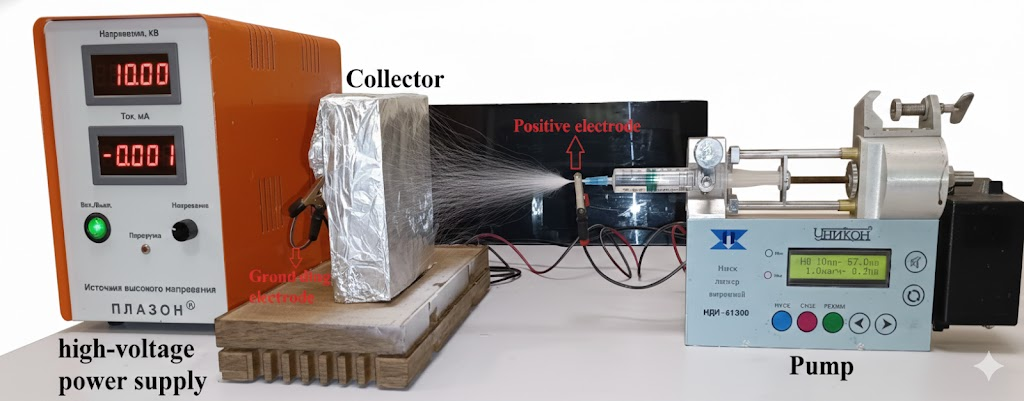
\includegraphics[width=0.5\linewidth]{electrosping machine...jpg}
\caption{Custom-built needle-based electrospinning setup.}
\label{fig:electrospinning setup}
\end{figure}

\section{Pre crosslinking}
\subsection{Thermal Treatment Protocol}
The as-spun PVA-CA nanofiber mats were subjected to crosslinking to render them water-insoluble. This crosslinking treatment involved a series of steps carried out in a laboratory oven (AB Utenos Elektrotechnika SNOL 58/350, AB Utenos Elektrotechnika, Lithuania), which has a temperature control system to \(\pm\)1\(^\circ\)C and a fan to circulate hot air for more efficient heating (Figure 3.4).

Crosslinking Steps:
1) Pre-Drying: Spun mats are placed on aluminum trays and dried at 60\(^\circ\)C for 30 minutes to dry out excess moisture without initiating crosslinking.
2) Crosslinking: Temperature is then set to 150\(^\circ\)C at a rate of 5\(^\circ\)C/min and maintained at this temperature for 60 minutes to allow crosslinking to occur completely without degrading the PVA matrix, as recommended by Parida et al.\cite{53} and Gohil and Ray.\cite{34}
3) Cooling: The oven is then allowed to cool down to a temperature lower than 50\(^\circ\)C before removal of the crosslinked mats.


\subsection{Chemical Mechanism of Esterification}
This crosslinking reaction is facilitated by Fischer esterification between citric acid’s –COOH groups and PVA’s –OH groups.\cite{96} Since citric acid is a tri-functional molecule, a 3D network is possible.\cite{50,51}
The reaction is:\\ PVA–OH + HOOC–CA \(\rightarrow\) PVA–O–CO–CA + H\(_2\)O \hfill (3.1)\\
This esterification reaction is facilitated by heat alone, with no need for any catalyst, especially at 150\(^\circ\)C. This high temperature is adequate to provide the activation energy required to activate the carboxylic acid group, allowing the PVA –OH groups to react.\cite{53,54} Water is the only by-product, thus adhering to green chemistry requirements. \cite{50}
Spectroscopic evidence of ester crosslinking is indicated by the presence of a carbonyl group between 1730-1733 cm\(^{-1}\), as discussed in Chapter 4.\cite{36,51}

\begin{figure}[h!]
\centering
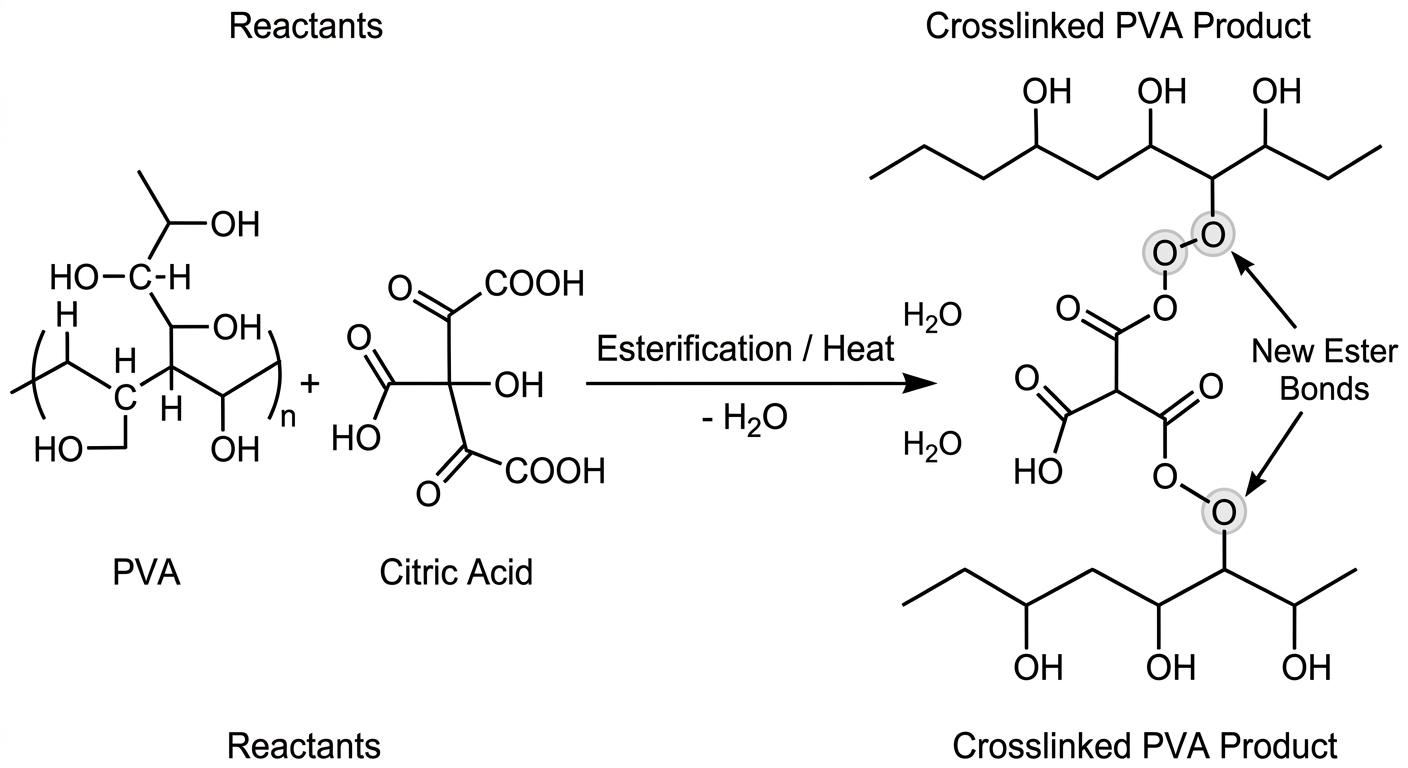
\includegraphics[width=0.8\linewidth]{esterification reaction.png}
\label{fig:crosslink-mechanism}
\end{figure}

\subsection{Mass Balance Quantification}
The degree of crosslinkeding was found by gravimetric analysis. The samples were weighed before (\(m_0\)) and after (\(m_1\)) the thermal treatment. The weight change, \(\Delta m\), is calculated as follows:
\[
\Delta m(\%) = \frac{m_0 - m_1}{m_0} \times 100 \tag{3.2}
\]
The mass loss of the samples is 8.3 \(\pm\) 0.4\% (n = 5), including the reaction water and the solvent, which evaporated during the treatment. This means that the citric acid carboxyl groups had reacted almost completely. \cite{53, 54}

\section{Membrane Functionalisation (Acid Doping)}
\subsection{Doping Solution Preparation}
Phosphoric acid dopant solutions were prepared by diluting 85 wt\% H\(_3\)PO\(_4\) solutions with deionized water to achieve 30 wt\%. This 30 wt\% H\(_3\)PO\(_4\) solution was chosen due to the results obtained in the initial screening, which showed a high conductivity enhancement without considerable membrane degradation.\cite{56,57}

\subsection{Kinetic Study of Acid Uptake}
A comprehensive study of kinetics was carried out to evaluate the mechanism by which acid absorption occurs and its impact on membrane properties. The membranes made from PVA-CA were subjected to a solution containing 30 wt\% H\(_3\)PO\(_4\) and kept at 25\(^\circ\)C for three different time intervals: 30 minutes, 2 hours, and 24 hours. These times correspond to the adsorption of acid molecules on the surface of the membrane within 30 minutes, followed by penetration into the membrane after 2 hours, and finally saturation of the membrane with acid after 24 hours.\cite{35,52} The acid uptake is defined by the following equation:
\[
AU = \frac{m_{d,t}-m_{d,0}}{m_{d,0}} \times 100 \tag{3.3}
\]

\subsection{Structural Integrity Limits}
The initial tests indicated that the use of more than 40 wt\% H\(_3\)PO\(_4\) resulted in the deterioration of the membrane. It swelled and lost its mechanical integrity and eventually dissolved after 1-2 hours. This is because of the acid-catalyzed hydrolysis of the ester crosslinks and the excessive plasticization of the PVA.\cite{35,58} In this study, the concentration of 30 wt\% has been chosen as a compromise.

\section{Analytical Characterization Techniques}
\subsection{Morphological Analysis (SEM)}
The shape of the fibers and the distribution of their diameters were studied using a Scanning electron microscope (SEM, TESCAN VEGA3, Czech Republic) with support from the NUST MISIS.

The instrument was operated in the following conditions: voltage - 5 kV, working distance - 4.63-8.74 mm, detector - secondary electron detector in high vacuum mode (\(<10^{-3}\) Pa).
For the preparation of the samples, the membrane was placed on a stub using conductive carbon tape and then subjected to a 10 nm thick gold coating using a QUORUM Q150R ES sputter coater to prevent charging during imaging in the SEM.\cite{39}
For the measurement of the diameters of the fibers, the images were taken at a magnification of 10,000\(\times\) using ImageJ (NIH, v1.54g). The diameters were measured at least five points in an image, with a minimum of 100 fibers.

\subsection{Chemical Footprint (FTIR-ATR)}
To verify the composition and crosslinking state, FTIR-ATR spectroscopy was used. The tests were carried out by LUCh Laboratory at NUST MISIS using a FTIR (ATP 8900, Optosky,Russia) spectrometer with a diamond ATR attachment. The parameters for collecting the spectra were as follows: scan range – 4000-400 cm\(^{-1}\), resolution – 4 cm\(^{-1}\), number of scans – 64.

A clear indication of crosslinking is seen in the ester carbonyl stretching region at approximately 1730-1733 cm\(^{-1}\). \cite{36,51} The bands can be attributed to the IR spectral characteristics of the specific groups in PVA and citric acid. \cite{69,70}

\subsection{Surface Wettability (Contact Angle)}
Static water contact angles were measured using a drop shape analyser located at NUST MISIS. A water droplet of 5 \(\mu\)L deionised water was placed on the surface of each membrane. 
The contact angle test device consisting of a high-resolution camera and a support to fix the sample. The camera
was placed on a movable rail and had two degrees of freedom (linear and rotary) to adjust focusing. At least five measurements were performed at different points on the surface of the membrane samples by dropping
a distilled water droplet using a micropipette onto the mat
surface and taking the photos, the contact angle values were
determined by marking five points on each droplet photo
using ImageJ software.The contact angles were then used to calculate the work of adhesion (Wa) and the surface free energy (\(\gamma\)).\cite{71}
\begin{figure}[h!]
\centering
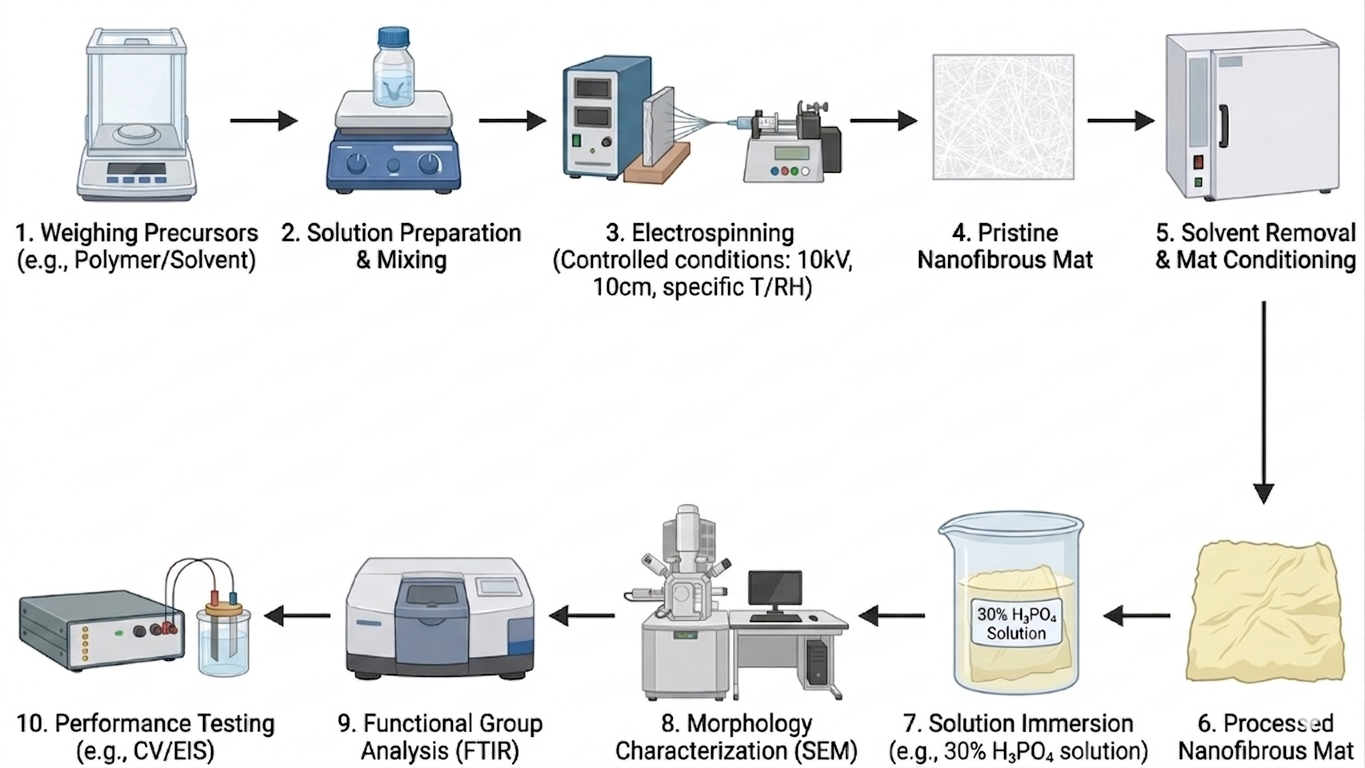
\includegraphics[width=0.8\linewidth]{fabrication and testing.png}
\caption{Fabrication and Characterization flow process of membrane}
\label{fig:Fabrication and Characterization flow process of membrane}
\end{figure}

\section{Computational Implementation}
\subsection{Theoretical Foundation: Density Functional Theory}
Density Functional Theory is the computational methodology employed in all calculations presented in this dissertation. Rather than solving the intractable many-body Schrodinger Equation, Density Functional Theory reformulates this problem in terms of the electron density, a three-dimensional quantity that is computationally tractable for systems of this size.\cite{72, 73} This reformulation is made possible by the Hohenberg-Kohn theorems, which prove that the ground-state energy of a system of electrons is a unique functional of the electron density, and the Kohn-Sham formulation that provides a concrete set of single-particle equations for solving this density in a self-consistent fashion.
The quality of a Density Functional Theory calculation is heavily dependent upon the choice of exchange-correlation functional that must be approximated in a calculation. Hybrid functionals, which combine a fraction of exact Hartree-Fock exchange with a Density Functional Theory correlation functional, have emerged as the most accurate class of functional for organic and polymer systems such as those studied in membrane-related research, offering a quality-to-cost ratio that cannot be achieved with either ab initio or semi-empirical methods.\cite{72, 73}

\subsection{Choice of Functional: B3LYP and Justification}
In this study, all the calculations are performed with the B3LYP functional. The B3LYP functional combines Becke's three-parameter exchange functional\cite{72} with the Lee-Yang-Parr correlation functional\cite{73} and also has 20\% exact exchange. This nonlocal exchange term is the distinguishing feature of the B3LYP functional compared with other GGA-based functionals. It is also the feature that allows the B3LYP functional to perform well for hydrogen-bonded organic systems. In the DFT framework, the partial covalency of the H-bond is typically over-delocalized. The nonlocal exchange term of the B3LYP functional is more accurate in this regard.

The B3LYP functional has been extensively validated in numerous studies of carbon-based systems with hydrogen, oxygen, and phosphorus.\cite{72,73} The relevant properties for this study—esterification energetics, H-bond binding energies, proton transfer barriers, and vibrational frequencies—can be obtained with the B3LYP functional with much less effort than the more accurate but more demanding coupled-cluster approaches.

\subsection{Dispersion Correction: Grimme D3BJ}
The common DFT functionals such as B3LYP do not include the London dispersion forces—those subtle but long-range correlations of the electrons. For the hydrogen-bonded systems such as PVA and H\(_3\)PO\(_4\), the dispersion forces act in conjunction with the electrostatic forces. Omission of the dispersion forces causes an error of 10-20 kJ/mol. \cite{74} Grimme’s third-generation dispersion correction D3 solves this problem by the inclusion of a pairwise term with first-principle-based coefficients and a three-body term for larger systems.\cite{74} The Becke-Johnson damping function prevents the double counting of the short-range correlations already included in the functional.\cite{75} B3LYP-D3BJ has become the standard for hydrogen-bonded organic systems and has been used throughout this study.

\subsection{Basis Set: 6-31G*}
The 6-31G* basis set was employed in all geometry optimizations, potential energy surface scans, frequency calculations, and single-point energy calculations within this dissertation.\cite{76} The 6-31G* basis set is a split valence double-zeta basis set that was first proposed by Hehre, Ditchfield, and Pople. It contains polarization functions on all heavy atoms. The polarization functions are important in order to reproduce the directional character of the electron density in hydrogen bonding and proton transfer reactions.\cite{76} Without polarization functions, hydrogen bonding would be poorly reproduced in both geometry and energy.

6-31G* provides reliable structural properties and energy values for the organic and organophosphorus compounds studied in this dissertation while at the same time avoiding the expense associated with triple-zeta basis sets. In consideration of the molecular models studied in this dissertation, which include a variety of compounds ranging from the PVA monomer and H\(_3\)PO\(_4\) species to the fully crosslinked wet assembly containing 65 atoms, 6-31G* is a proper basis set that balances both efficiency and reliability.

\subsection{Software: ORCA 6.1.1}
For all quantum-chemical calculations, we used version 6.1.1 of the ORCA program, which has been developed at the Max Planck Institute for Chemical Energy Conversion by Neese et al.\cite{77,78,79} This program allows access to the entire range of DFT functionals, basis sets, as well as to property calculations, which we required, within a single program.

The calculations were carried out on a Windows workstation (INBOOK X2) with 4 MPI parallel processes, a 4-core CPU, and 16 GB of RAM available. To accelerate calculations of coulomb and exchange integrals without compromising their precision, we applied the RIJCOSX method.\cite{80} The B3LYP-D3BJ/6-31G* method in combination with version 6.1.1 of the ORCA program is a well-established, reproducible protocol for hydrogen-bonded organic systems.

\subsection{Molecular Models: PVA Monomer, CA, H\(_3\)PO\(_4\), and Crosslinked Units}
The molecular models maintain the key chemical properties of the PVA/CA/H\(_3\)PO\(_4\) membrane system while keeping the system tractable for DFT calculations. Isopropanol is used as a substitute for PVA, as it retains the pendant secondary alcohol functional group present in the repeating unit of PVA but does not have to simulate an entire polymer chain, as is common in cluster-based DFT studies of polymers.\cite{18,19} Citric acid is represented as its neutral tricarboxylic acid form. The ester crosslink is formed by covalently attaching the carboxyl functional group of citric acid to the hydroxyl functional group of the PVA monomer unit. This structure is fully optimized.

The most complex system is referred to as CalcNew2 and contains two PVA monomer units bonded by an ester crosslink formed by citric acid, two H\(_3\)PO\(_4\) molecules, and three water molecules. This cluster contains a total of 65 atoms and is approximately 800 Da in mass. This system is representative of a single crosslink site in the hydrated doped membrane system and is the most realistic finite cluster for the membrane system that is tractable for B3LYP-D3BJ/6-31G* calculations.

\subsection{Calculations:Geometry Optimisation, PES Scan, TS, NBO, ELF, and NEB}
Geometry optimisations were carried out for each molecular model to find energy-minimised ground states using the BFGS algorithm with tight convergence criteria.\cite{81} To explore the potential energy surface (PES), we fixed a relevant bond coordinate at specified intervals and allowed other degrees of freedom to relax to obtain a profile from which the transfer barrier is obtained. Three scans were carried out: a gas-phase proton transfer process (15 steps), desorption of H\(_3\)PO\(_4\) from PVA (20 steps), and a proton transfer process in a fully crosslinked wet system - CalcNew3 (15 steps). To obtain transition states (TS), a quasi-Newton eigenvector-following method was used, followed by frequency analysis to confirm that precisely one imaginary vibrational mode is present along the reaction coordinate, fulfilling the first-order saddle point criterion.\cite{81,82,83}
We have performed natural bond orbital (NBO) calculations at critical geometries to obtain bond orders, charges, and donor-acceptor orbital interaction energies, providing direct electronic evidence of the Grotthuss mechanism.\cite{84,85}
We have also computed the electron localisation function (ELF) at the transition-state structure to obtain insight into the spatial arrangement of electron localisation, aiding the differentiation between Grotthuss hopping and vehicular transport by examining the topology of electron localisation basins.\cite{86,87,88}
To verify the minimum-energy pathway of proton transfer, eliminating possible alternative mechanisms, we have carried out nudged elastic band (NEB) calculations using eight images.\cite{89,90,91}
To obtain temperature-dependent Gibbs free energy corrections, harmonic frequency calculations were used, providing us with access to statistical thermodynamics to determine \(\Delta G^{\ddagger}(T)\) and \(k(T)\) at the fuel cell temperatures.\cite{92,93}

\subsection{Binding Energy, Frequency Scaling, and BSSE Correction}
The binding energies were calculated by taking the energy of the optimized complex and subtracting the combined energy of the separated fragments:
\[
\Delta E_{\text{bind}} = E(\text{complex}) - \sum E(\text{components}) \tag{3.7}
\]

The harmonic vibrational frequencies were multiplied by a scaling factor of 0.9614, which is the standard correction factor for B3LYP with a double-zeta basis set as recommended by Scott and Radom\cite{94} for correcting anharmonic effects and the overestimation inherent in the harmonic approximation.

The counterpoise correction for BSSE is not included in the calculations because it is typically below 3 kJ/mol for representative complexes using the Boys-Bernardi\cite{95} method. This is within the acceptable limit for this comparative analysis. Thus, corrections for BSSE are not included in this level of theory.\cite{18,19}

\subsection{Limitations of the Gas-Phase DFT Approach}
All of the calculations presented in this dissertation were performed on a gas-phase system, employing a finite molecular cluster model. This allows us to isolate the essential quantum mechanical interactions between molecules, without the complicating effects of the real-world membrane system in a condensed phase state. That is, the binding energies and transfer barriers calculated in this gas-phase system are not to be taken as those which would occur in a real-world system—in a real-world system, the effects of a solvent/dielectric would tend to reduce both binding energies and transfer barriers relative to their gas-phase counterparts. \cite{18,19}
Nevertheless, the major findings of this work, the relative results across the systems, the mechanism of the proton transfer process, and the arrangement of the calculated barriers in relation to the experimental activation energies all hold within the gas-phase cluster formalism. This is the standard playbook in computational membrane science, the foundation for all DFT-based work on Nafion, PBI, and sulfonated polymers that constitutes the established body of work in the field.\cite{18,19,20} In Chapter 6, we discuss the potential for future work in the corrections for the condensed phase via implicit solvent and periodic DFT.

\subsection{Covalent Phosphorylation Study: Computational 
Design of a Leach-Proof Membrane}

\subsubsection{Motivation and Scope}

The 23 calculations described above establish the molecular 
mechanisms of the experimentally fabricated non-covalent 
PVA/CA/H\(_3\)PO\(_4\) system. A central finding of that 
work is that approximately 66\% of the incorporated 
phosphoric acid sits at single-site hydrogen-bond positions 
and is displaced by water during washing, leaving only 34\% 
retained in the membrane. This vulnerability is intrinsic 
to non-covalent binding: water molecules can compete for 
the same hydroxyl sites that hold the acid.

A direct computational remedy is to ask whether replacing 
the hydrogen bond between phosphoric acid and the PVA 
backbone with a covalent P--O--C phosphate ester linkage 
would eliminate this leaching pathway. Phosphorylated PVA 
has been prepared experimentally using phosphoryl chloride 
and phosphoric acid with urea as a coupling agent, but no 
quantum-mechanical study had previously determined whether 
covalent anchoring preserves or diminishes the proton 
donor activity of the remaining P--OH groups. Eight 
additional DFT calculations were therefore performed to 
answer this question directly, bringing the total 
calculation count in this dissertation to 31.

\subsubsection{Model Construction}

The same computational framework used for the non-covalent 
study was applied throughout: B3LYP-D3BJ/6-31G*/ORCA~6.1.1. 
The PVA repeat unit was again represented as isopropanol. 
The covalent monomer was constructed by replacing the 
hydroxyl hydrogen of isopropanol with a 
$-$P($=$O)(OH)$_2$ group, giving a 17-atom phosphate 
monoester (C$_3$H$_9$O$_4$P) with a direct P--O--C bond. 
This models the product of a Fischer-type esterification 
between phosphoric acid and the PVA backbone hydroxyl 
group. The non-covalent hydrogen-bonded complex from the 
first study (isopropanol + H\(_3\)PO\(_4\)) served as the 
reference in all comparisons so that both binding modes 
were treated at exactly the same level of theory.

\subsubsection{Calculations Performed}

Eight calculations were carried out as listed in 
Table~3.2. Geometry optimisations used TightOpt convergence 
for all monomer and binary systems. The large membrane 
assembly used LooseOpt thresholds, consistent with the 
approach applied in CalcNew2 of the first study.

\begin{table}[h!]
\centering
\caption{Summary of covalent phosphorylation calculations 
(B3LYP-D3BJ/6-31G*/ORCA~6.1.1).}
\label{tab:covalent-calcs}
\begin{tabular}{c l l l}
\toprule
Calc & System & Type & Key output \\
\midrule
C1 & Covalent monomer & Optimisation & 
P--O--C = 1.612~\AA{} \\
C2 & Covalent monomer + 3H\(_2\)O & Hydration energy & 
$\Delta E = -192.8$~kJ\,mol\(^{-1}\) \\
C3 & Covalent monomer & Desorption PES (20 steps) & 
Barrier = $+251.9$~kJ\,mol\(^{-1}\) \\
C4 & Covalent monomer + acceptor & Proton transfer PES & 
Barrier = $+38.2$~kJ\,mol\(^{-1}\) \\
C5 & Covalent monomer & Bond orders, CHELPG charges & 
P--O bond order = 1.015 \\
C6 & Non-covalent reference & Bond orders, CHELPG charges & 
P$\cdots$O bond order $\approx$ 0.05 \\
C7 & 62-atom covalent membrane & Optimisation & 
$E = -2511.232$~E\(_h\) \\
C8 & 65-atom non-covalent membrane & 50~ps MD stability & 
Network stable \\
\bottomrule
\end{tabular}
\end{table}

\subsubsection{Desorption and Proton Transfer Scans}

Desorption potential energy surfaces were obtained as 
relaxed scans in which every coordinate except the one 
being stepped was re-optimised at each point. For the 
covalent system the P--O bond distance was stepped from 
1.612 to 4.500~\AA{} in 20 equal increments. For the 
non-covalent reference the P$\cdots$O separation was 
stepped from 3.169 to 9.000~\AA{} in 20 steps, consistent 
with the desorption scan performed in the first study. 
Both curves were set to zero energy at their respective 
equilibrium geometries so that the desorption barriers 
are directly comparable.

Proton transfer scans were performed with a second 
isopropanol molecule acting as the proton acceptor in 
both cases. For the non-covalent system the O--H donor 
distance was scanned in 15 steps from 0.980 to 1.750~\AA{}. 
For the covalent system the H$\cdots$O(acceptor) distance 
was scanned in two segments: 13 steps from 1.750 to 
1.528~\AA{} and 8 steps from 1.528 to 0.972~\AA{}, covering 
the full transfer pathway including the shallow 
shared-proton intermediate identified during the scan.

\subsubsection{Electronic Analysis}

Mayer bond orders and CHELPG electrostatic charges were 
computed at every converged geometry. Mayer bond orders 
quantify the covalent character of a bond on a scale from 
0 (no bond) to 1 (full single bond) and above, making 
them the appropriate descriptor for comparing a hydrogen 
bond (bond order $\sim$0.05) with a covalent P--O--C link 
(bond order $\sim$1.0). CHELPG charges were used to 
monitor the charge on the transferring proton across the 
two binding modes, since a more positive proton is a more 
readily released proton. NBO analysis and ELF mapping 
were computed at the transition state geometries of both 
proton transfer scans to confirm the Grotthuss hopping 
signature in both systems.

\subsubsection{Full Membrane Model}

To test whether the covalent P--O--C bonds survive in a 
realistic membrane environment, a 62-atom assembly was 
constructed containing two covalently phosphorylated PVA 
units joined by a citric acid ester crosslink, with three 
explicit water molecules occupying the pore space. This 
model is the covalent analogue of the CalcNew2 assembly 
used in the first study and was built from the same 
citric acid crosslinked framework. The geometry was 
fully relaxed using LooseOpt thresholds. Bond lengths and 
hydrogen bond geometries in the converged structure were 
compared with the isolated covalent monomer and with 
crystallographic reference values for phosphate monoesters 
to assess whether the membrane environment distorts or 
preserves the covalent linkage.

\subsubsection{Limitations}

The same gas-phase cluster limitations that apply to the 
first study apply here. All calculations are performed on 
finite molecular models without long-range electrostatics, 
condensed-phase dielectric effects, or polymer chain 
dynamics. Because both binding modes are treated with 
exactly the same method and basis set, systematic errors 
cancel in the comparison and the qualitative conclusions 
— that covalent anchoring dramatically raises the 
desorption barrier while leaving proton donor activity 
unchanged — should hold at higher levels of theory. 
Experimental synthesis and electrochemical testing of 
covalently phosphorylated PVA membranes remains the 
necessary next step for validation.

\subsection{Molecular Dynamics Setup (LAMMPS)}

\subsubsection{Force Field and System Construction}

Classical molecular dynamics simulations were performed using LAMMPS 
(Large-scale Atomic/Massively Parallel Simulator, version 29 September 
2021) \cite{104}. The simulation system was built directly 
from the DFT-optimised Calc07 geometry --- a 52-atom crosslinked 
membrane fragment comprising two PVA monomers, a citric acid 
crosslinker, and two covalently bound phosphate groups --- so that 
the MD starting structure was fully consistent with the quantum 
mechanical reference. All membrane atoms were described by the 
OPLS-AA (Optimised Potentials for Liquid Simulations, All-Atom) force 
field \cite{95}. Atom types were assigned from the DFT 
connectivity analysis: alkyl CH carbons as opls\_135/137, bridging 
phosphate oxygen as opls\_480, phosphorus as opls\_479, P\(=\)O oxygen 
as opls\_481, P--OH oxygen as opls\_482, ester carbonyl carbon as 
opls\_235, and ester C\(=\)O oxygen as opls\_236. Water was represented 
by the SPC/E model \cite{107}, which reproduces the 
self-diffusion coefficient and dielectric constant of liquid water 
accurately at 353 K. One hundred and fifty SPC/E water molecules were 
placed randomly in the simulation box with a minimum separation of 
2.5~\AA{} from any existing atom, yielding a total system of 547 atoms 
in a cubic periodic box of edge length 50.54~\AA{}. The pair 
interaction cutoff was set to 6.0~\AA{}, satisfying the requirement 
that the cutoff must not exceed half the box length to avoid periodic 
self-interaction.

\subsubsection{Force Field Validation}

Before any dynamics, the system was energy-minimised and the resulting 
bond lengths were compared against DFT reference values from Calc01 
(B3LYP-D3BJ/6-31G*/ORCA~6.1.1). The P--O--C bridge bond length 
converged to 1.623~\AA{} (DFT: 1.612~\AA{}, deviation $+0.7$\%), 
C--O--P carbon-side bond to 1.441~\AA{} (DFT: 1.465~\AA{}, 
$-1.6$\%), P\(=\)O to 1.480~\AA{} (DFT: 1.475~\AA{}, $+0.3$\%), 
and O--H phosphate to 0.967~\AA{} (DFT: 0.972~\AA{}, $-0.5$\%). 
All deviations fall within the accepted \(\pm\)0.05~\AA{} threshold 
for OPLS-AA validation \cite{95}, confirming that the 
force field faithfully represents the covalent P--O--C architecture 
established by DFT.

\subsubsection{Equilibration and Production Protocol}

The system was equilibrated through five sequential NVT stages using 
a Nos\'{e}--Hoover thermostat with an additional velocity rescaling 
fix (temp/rescale) applied every 10--100 steps to prevent kinetic 
energy explosions during heating: 1~K to 10~K at 0.1~fs timestep 
over 10~ps; 10~K to 50~K at 0.2~fs over 10~ps; 50~K to 150~K at 
0.5~fs over 25~ps; 150~K to 353.15~K at 1.0~fs over 50~ps; and a 
final hold at 353.15~K for 100~ps. This staged heating protocol 
is necessary for polymer systems where large velocity gradients 
at the start of dynamics can destabilise intramolecular bond 
interactions \cite{104}. Following equilibration, a 
500~ps production run was performed at 353.15~K with a 1.0~fs 
timestep. Atomic coordinates were written every 1~ps for trajectory 
analysis.

\subsubsection{Computed Quantities}

Two quantities were extracted from the production trajectory. The 
mean square displacement (MSD) of phosphorus atoms was computed using 
the \texttt{compute msd} command with centre-of-mass correction, 
time-averaged every 100 steps. A bounded MSD — showing no sustained 
linear growth — indicates that the phosphate group is covalently 
anchored and not diffusing, which is the expected signature of acid 
retention. A linearly growing MSD would indicate free diffusion 
and acid leaching \cite{64}. The radial distribution 
function g(r) between phosphorus atoms (type~5) and bridging oxygen 
atoms (type~4) was computed using \texttt{compute rdf} with 100 bins, 
time-averaged over the full 500~ps production run, to monitor the 
structural integrity of the P--O--C covalent linkage.

\subsection{Macroscopic Device Modelling (COMSOL Multiphysics)}

\subsubsection{Model Geometry and Physics}

A two-dimensional single-cell PEMFC model was implemented in COMSOL 
Multiphysics 6.3 using the Secondary Current Distribution interface, 
which solves the conservation of ionic and electronic current with 
Butler--Volmer electrode kinetics. The model geometry consisted of 
a single membrane domain of thickness 50~\(\mu\)m (consistent with 
SEM cross-section measurements of the 24~h doped sample) and width 
100~\(\mu\)m, bounded by anode and cathode current collector 
boundaries.

The membrane domain was governed by:

\begin{equation}
\nabla \cdot \left( \sigma_{m} \nabla \phi_{m} \right) = 0
\end{equation}

Electrode reactions at the anode (hydrogen oxidation) and cathode 
(oxygen reduction) were described by the Butler--Volmer equation:

\begin{equation}
i = i_0 \left[ 
\exp\!\left(\frac{\alpha_a F \eta}{RT}\right) - 
\exp\!\left(-\frac{\alpha_c F \eta}{RT}\right) 
\right]
\end{equation}

where \(i_0 = 10^{-3}\)~A\,m\(^{-2}\) is the exchange current 
density, \(\alpha_a = \alpha_c = 0.5\) are symmetric transfer 
coefficients, \(F\) is Faraday's constant, \(R\) is the gas 
constant, and \(T = 353.15\)~K.

\subsubsection{Input Parameters and Limitations}

The membrane proton conductivity was set to 
\(\sigma_{m} = 35\)~mS\,cm\(^{-1}\), taken from published values 
for comparable PVA/H\(_3\)PO\(_4\) membrane systems reported at 
similar doping levels \cite{110}, as the experimental EIS 
measurements for the present samples are currently in progress 
(Appendix~D). This value is consistent with the preliminary 
conductivity estimates presented in Table~D.1. The model will be 
reparameterised with the experimentally measured conductivity upon 
completion of EIS characterisation, which is expected to refine the 
quantitative outputs while leaving the qualitative trends and 
structural conclusions unchanged. All other boundary conditions 
and solver settings are documented in Appendix~F.

\chapter{Experimental Results and Discussion}

This section presents the experimental characterization of the electrospun membrane series made from the PVA/CA/H\(_3\)PO\(_4\) blend system, which was subjected to four different doping time conditions: the undoped and crosslinked membrane (S0), the membrane subjected to the doping process for 30 minutes (S1), the membrane subjected to the doping process for 2 hours (S2), and the membrane subjected to the doping process for 24 hours (S3). Each of the four techniques employed in the characterization of the electrospun membrane series is presented as a separate part, with the results and discussions woven together accordingly. Where applicable, the discussions are related to the DFT results presented in Chapter 5.

\section{Scanning Electron Microscopy (SEM)}

\subsection{Quantitative Fiber Diameter Distribution}

To establish a structural baseline for the membrane series, the fiber diameters of the as-spun, thermally crosslinked S0 sample were statistically analyzed. Figure 4.1 presents the diameter distribution derived from multiple high-magnification SEM micrographs. The fibers demonstrate a remarkably consistent morphology, with the majority of diameters falling within the 200--300 nm range.

The calculated mean diameter of approximately 256 nm suggests that the electrospinning parameters—specifically the voltage and flow rate—were well-optimized for the PVA/CA blend viscosity. This sub-micron scale is essential for the membrane's functionality, as it creates a high specific surface area. From a transport perspective, this fine fiber architecture ensures that during the subsequent doping stages, the phosphoric acid has immediate and uniform access to the polymer chains, facilitating efficient infiltration into the amorphous regions of the PVA matrix.


\subsection{Membrane Morphology Evolution — SEM Analysis}
For the study of the changes in the membrane’s morphology during the entire range of doping times, scanning electron microscopy was utilized. In the study, two different magnification values were used in taking the SEM images of the samples, with the objective of capturing the overall membrane structure as well as the detailed structure at the fibre and film levels. The entire set of SEM images is shown in Figure 4.1.\cite{39}

\subsection{S0 (Undoped Membrane): Pristine Nanofibrous Topology}
The morphological evolution of the series begins with the S0 membrane, which represents the state of the material after electrospinning and thermal curing, but prior to any acid exposure. As seen in the SEM micrographs in Figure 4.2, the membrane possesses a classic non-woven, "spaghetti-like" architecture. The fibers are characterized by their smooth, cylindrical surfaces and are free from "beads" or structural defects that often plague unoptimized electrospun polymers.

Crucially, the fibers remain individually distinct and randomly overlapped, maintaining a highly porous and open interconnected network. This confirms that the thermal crosslinking at 150$^\circ$C successfully induced esterification between the PVA hydroxyl groups and Citric Acid carboxyl groups without causing the fibers to melt or lose their 1D geometry. This pristine topology is structurally robust; it provides the necessary mechanical framework to withstand the initial plasticization that occurs when the doping process begins, as described in the following sections for samples S1 through S3.
% --- Fiber Diameter Histogram ---
\begin{figure}[h!]
    \centering
    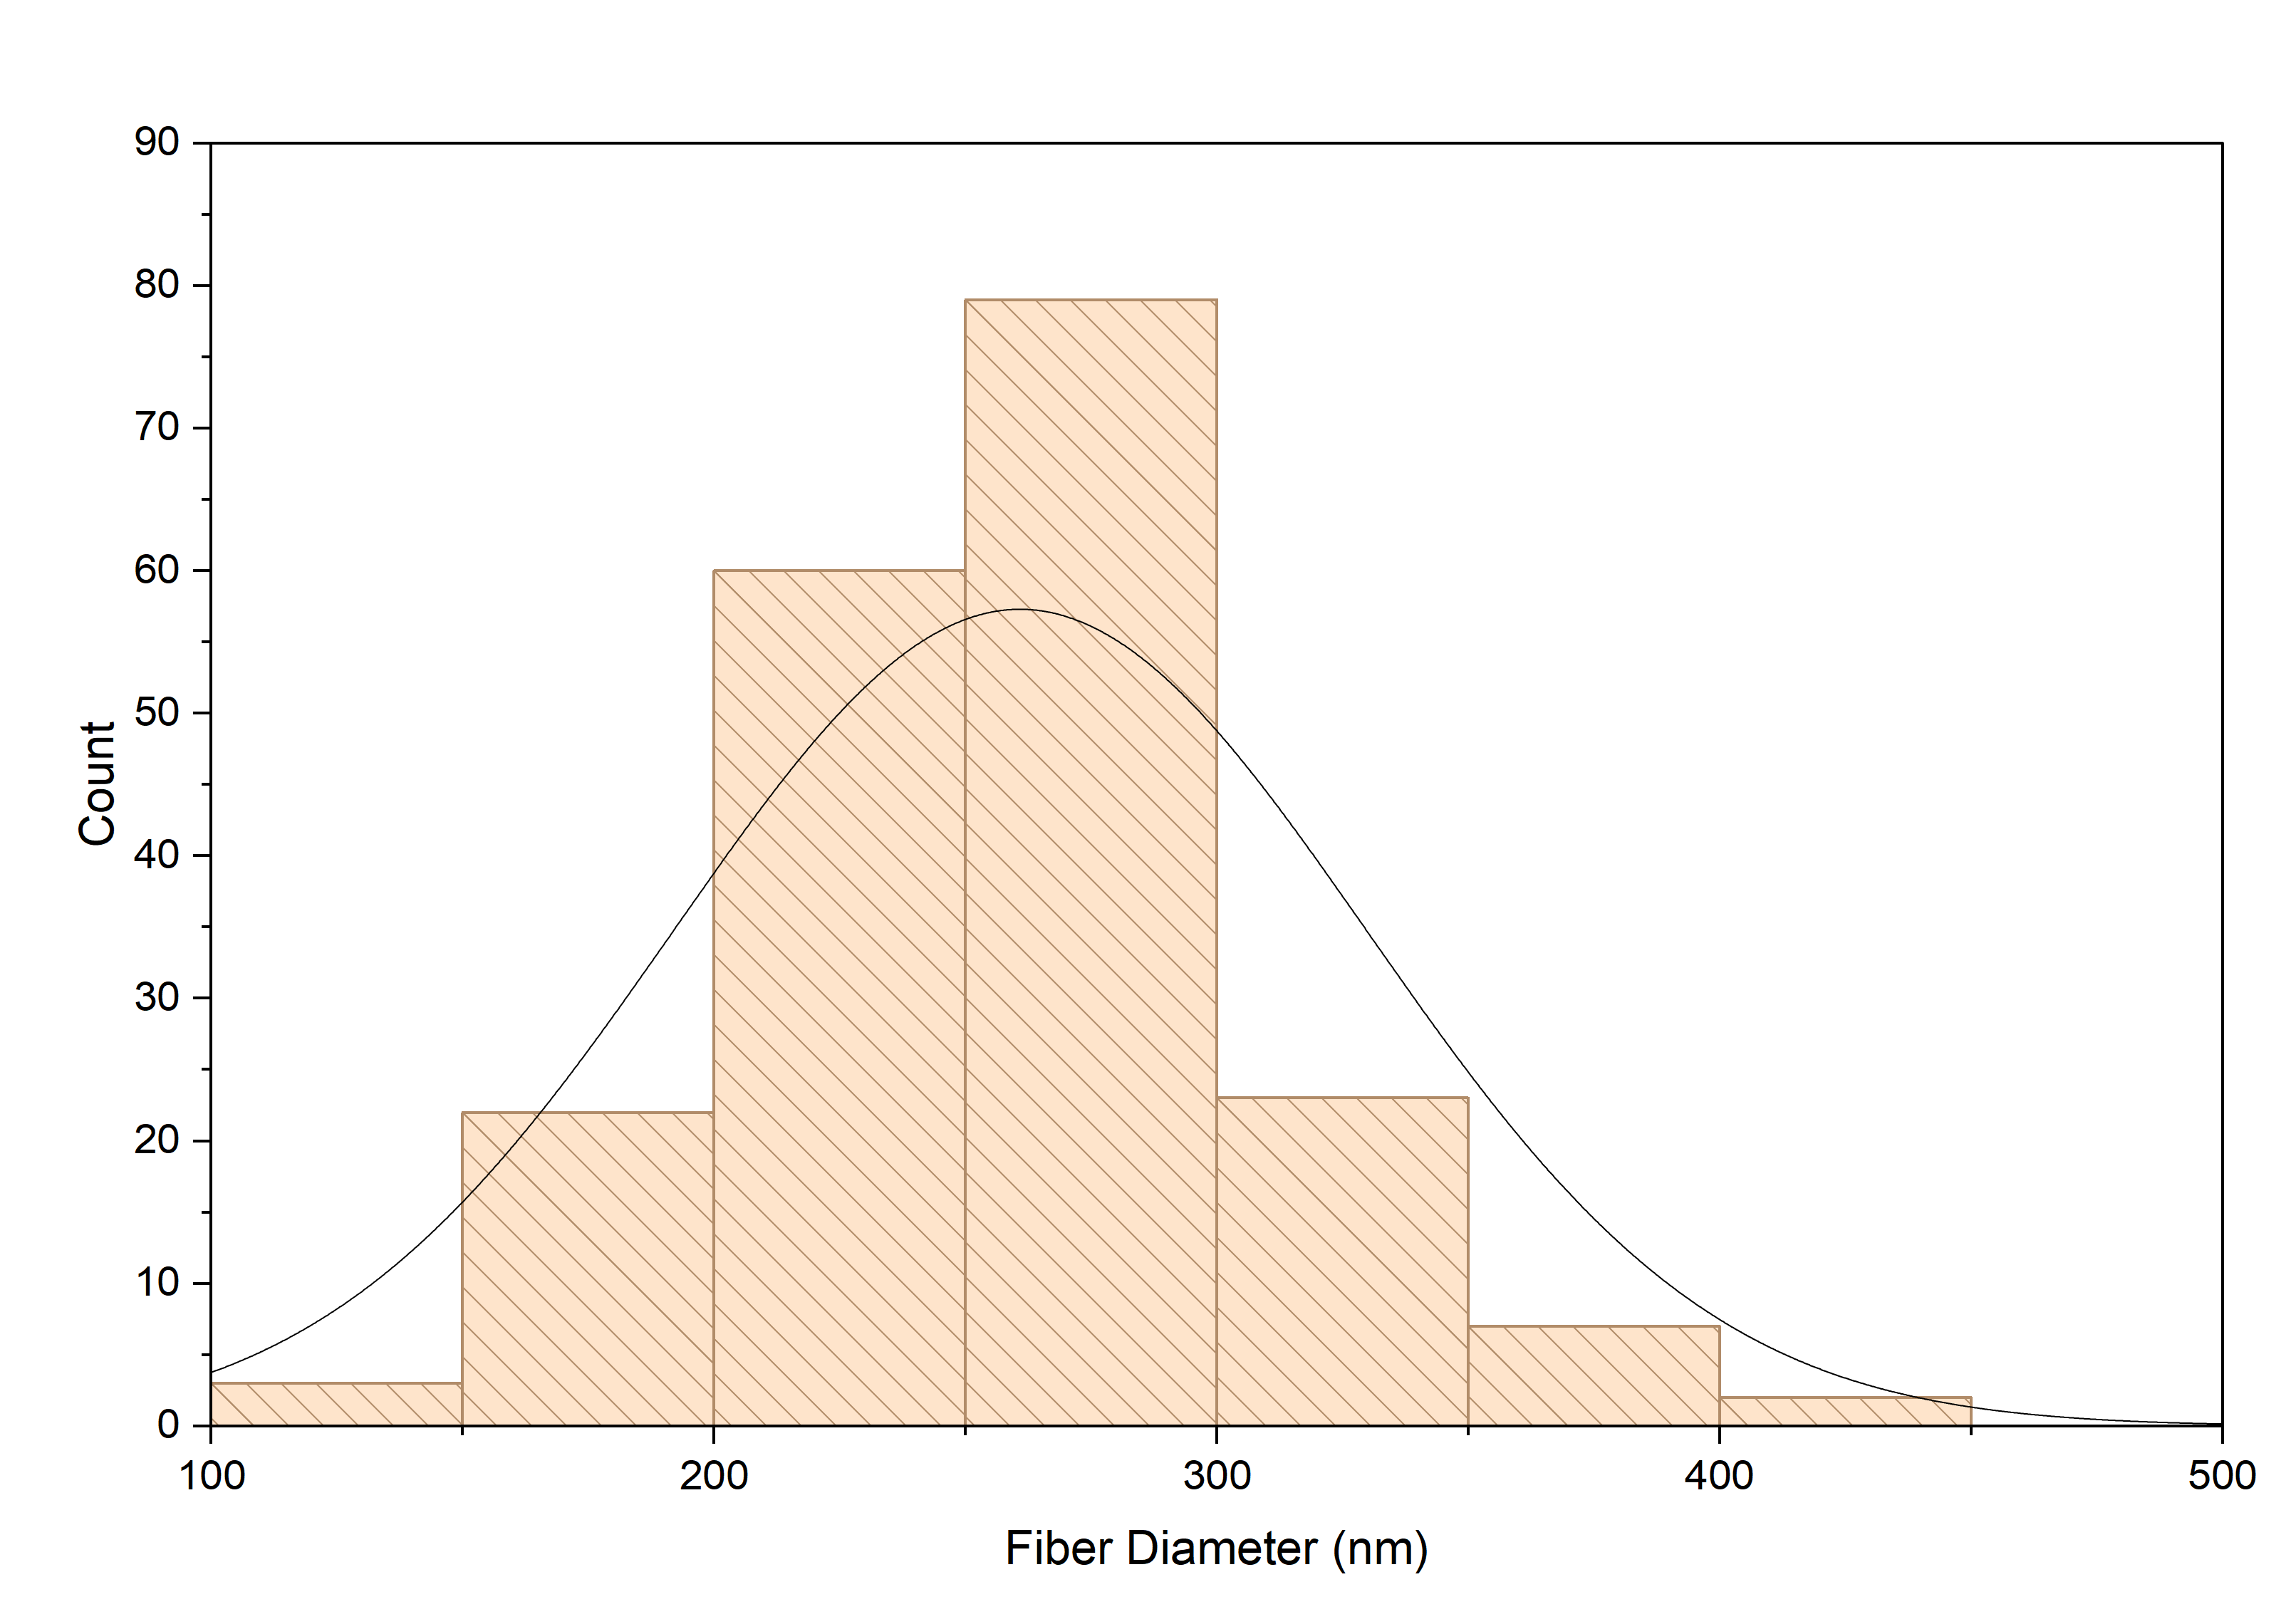
\includegraphics[width=0.75\linewidth]{5-2 Fiber diamter_both images final nm final.png} 
    \caption{Frequency distribution of fiber diameters for the S0 membrane, showing a well-defined nanometric scale centered near 256 nm.}
    \label{fig:histogram}
\end{figure}

% --- S0 SEM Images ---
\begin{figure}[h!]
    \centering
    \begin{subfigure}{0.48\linewidth}
        \centering
        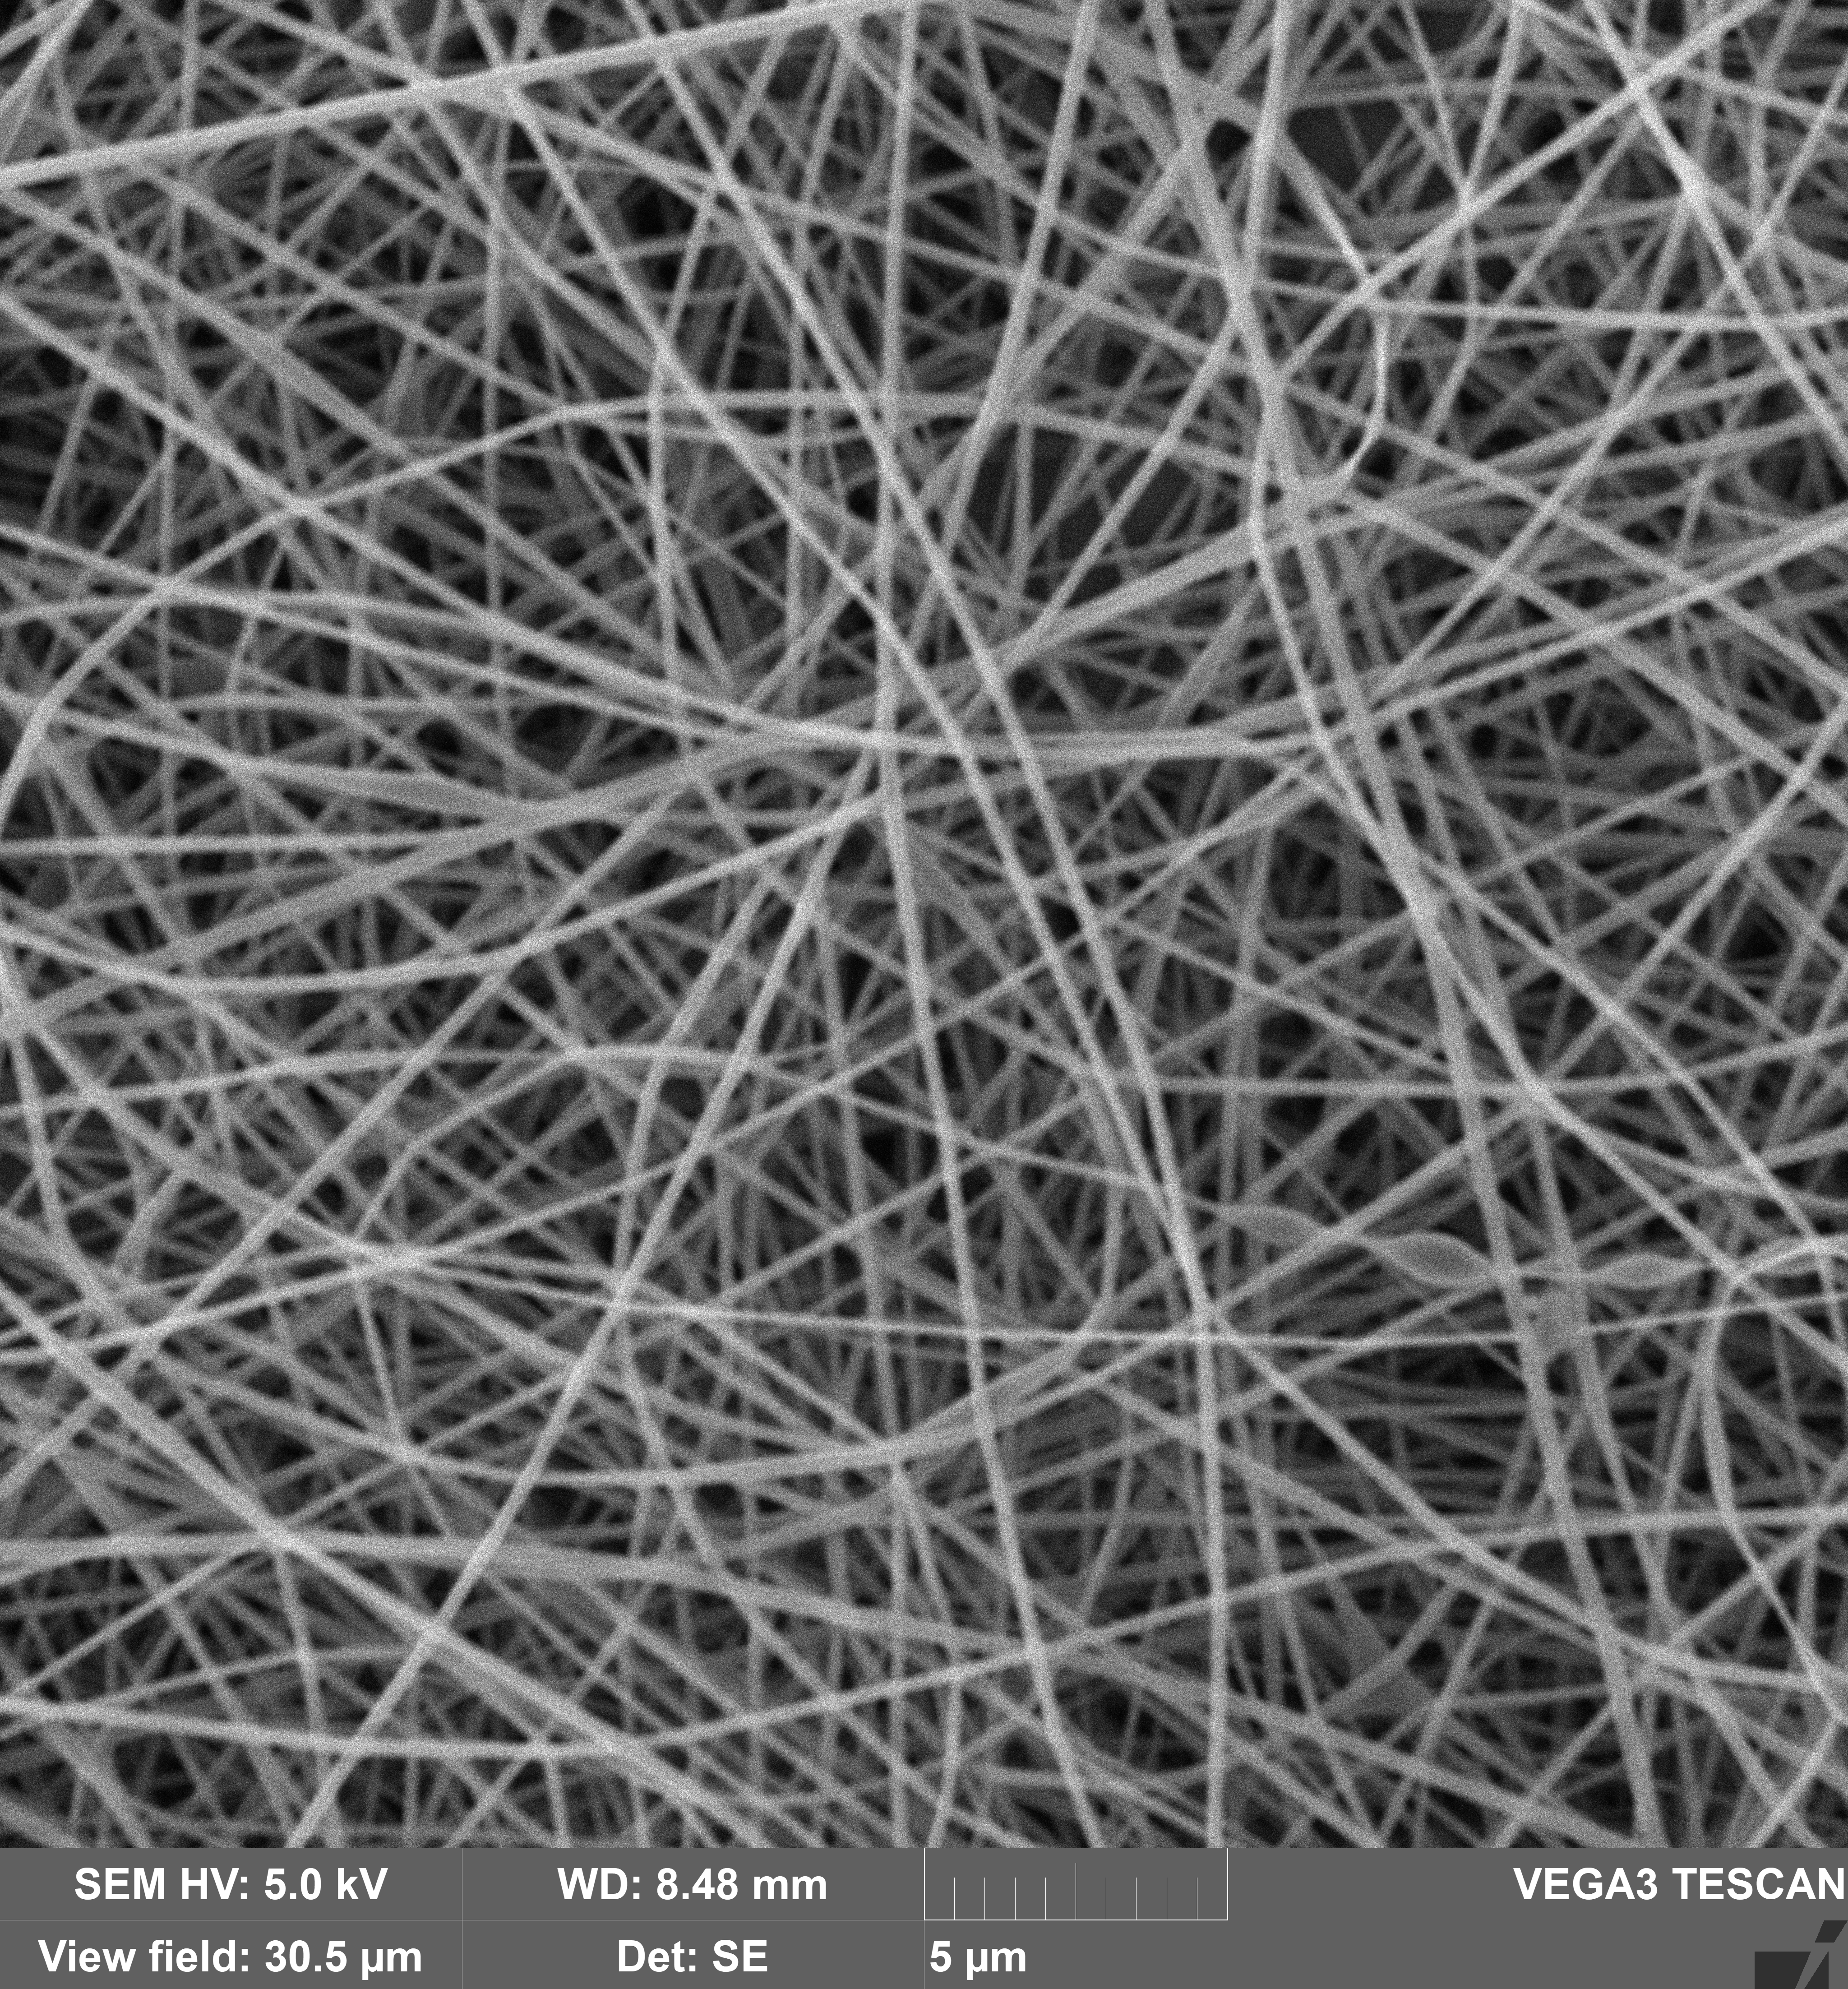
\includegraphics[width=\textwidth]{0.png} 
        \caption{S0 (Pristine), Low Magnification}
    \end{subfigure}
    \hfill
    \begin{subfigure}{0.48\linewidth}
        \centering
        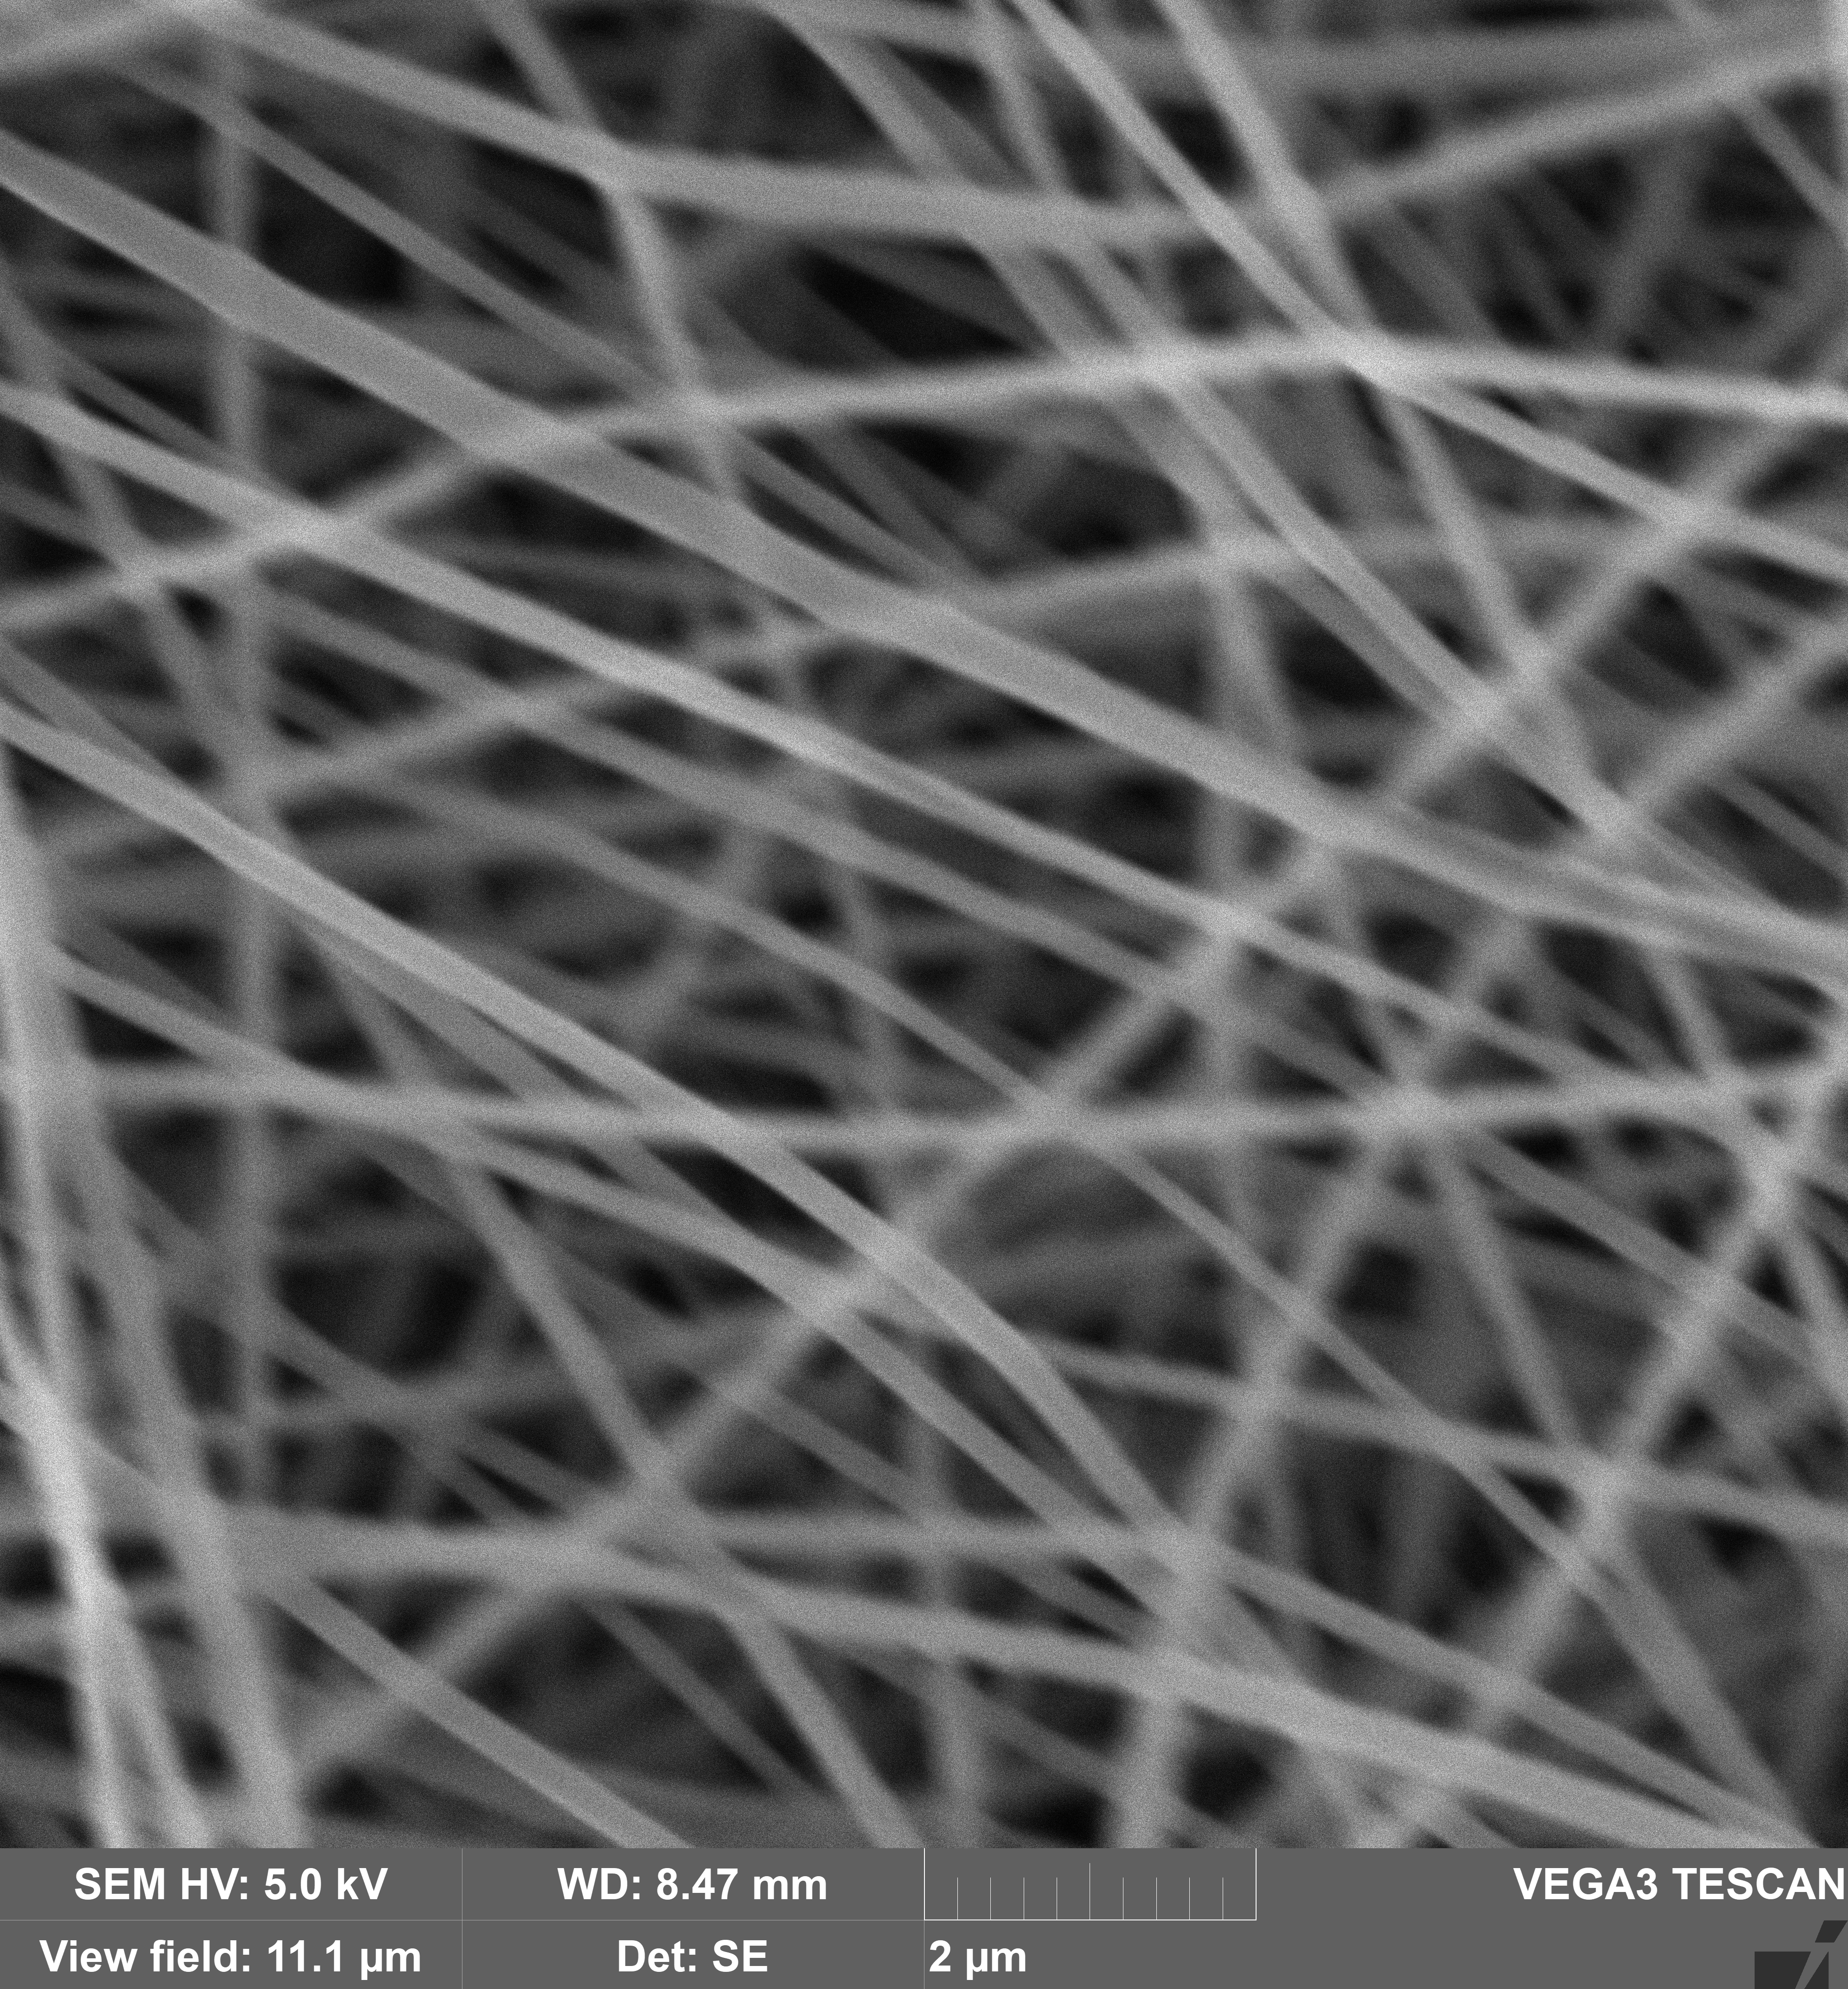
\includegraphics[width=\textwidth]{zero.png} 
        \caption{S0 (Pristine), High Magnification}
    \end{subfigure}
    \caption{SEM micrographs of the crosslinked PVA/CA membrane (S0) showcasing the open pore structure and fiber integrity prior to $H_3PO_4$ doping.}
    \label{fig:sem_s0}
\end{figure}

\subsection{S1 (30 Minutes Doping): Early Surface Swelling and Acid Uptake}
The S1 membrane, after the 30 minutes doping, has maintained its obviously fibrous appearance after the electrospinning step. It is possible to distinguish the fibers, although the surface of the fibers swells slightly, indicating the initial infiltration of phosphoric acid into the amorphous regions of the crosslinked PVA network. The membrane structure has been preserved, implying that the network of ester crosslinkeds developed after thermal curing at 150\(^\circ\)C is sufficiently robust to prevent significant changes in membrane structure after short periods of doping.\cite{53, 54}
The small swelling that occurs at this time is consistent with the known plasticizing effect of phosphoric acid on such PVA matrices, as the molecules insert themselves between the chains in the amorphous regions of the matrix, breaking the hydrogen bonds between chains that maintain the shape of the fiber, effectively reducing the glass transition temperature locally enough to allow some relaxation of the chains to occur.\cite{35,52} The pore structure remains open at this time, which is important in terms of transport properties – the accessible pore structure maximizes the hydroxyl groups accessible to the doping solution and also allows the phosphoric acid molecules access to the binding sites across the full depth of the membrane, not just the surface.

\subsection{S2 (2 Hours Doping): Progressive Plasticisation and Fibre Coalescence}
After two hours of doping with the S2 membrane, its shape is very different from the one observed before. The boundaries between the fibers, which were still apparent at the 30-minute mark, begin to crumble, and the fibers next to each other are seen to merge at the points where they touch one another. This is consistent with the increasingly plasticized nature of the PVA matrix due to the phosphoric acid doping. As the phosphoric acid absorbs deeper and deeper into the amorphous regions of the matrix, the glass transition temperature continues to be lowered, allowing the polymer chains to relax and the fibers to merge at the points where they touch one another.\cite{4,35}

The network becomes partially collapsed, somewhat porous, but no longer maintains that neat structure of individual fibers that was obtained with the shorter doping time. This change in structure has an immediate electrochemical consequence, as more continuous pathways of acid-rich material form through the thickness of the membrane with the collapse of these fiber boundaries, helping to explain the increase in conductivity observed between S1 and S2 in the EIS results presented in Section 4.4.\cite{52, 58}

\subsection{S3 (24 Hours Doping): Complete Fibre Fusion and Dense Film Formation}
The change in shape is complete after 24 hours of doping. The S3 membrane has transformed into a dense film with a seamless structure, where individual fibers cannot be distinguished because they have all come together to form one homogeneous polymer matrix with phosphoric acid. The change represents a complete transformation away from the nanofibrous structure, but this is when maximum conductivity is achieved.\cite{52,58}

The SEM progression, from open fibrous structure at 30 minutes to partially coalesced structure at 2 hours, to dense film at 24 hours, clearly illustrates that the doping time is a parameter that can be controlled to influence the structure of the membranes. The dense film structure in S3 eliminates the high resistance fibre-to-fibre junctions that would otherwise interrupt the continuity of proton transport pathways in the less-doped membranes. This is consistent with the progressive reduction in activation energy indicated by the EIS results.\cite{35,52,58}

\begin{figure}[h!]
\centering
% Top row: Low magnification images
\begin{subfigure}{0.32\linewidth}
\centering
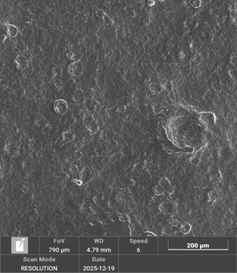
\includegraphics[width=\textwidth]{1.30.png}
\caption{30 min, low mag}
\end{subfigure}%
\begin{subfigure}{0.32\linewidth}
\centering
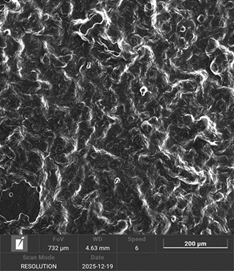
\includegraphics[width=\textwidth]{3.png}
\caption{2 h, low mag}
\end{subfigure}%
\begin{subfigure}{0.32\linewidth}
\centering
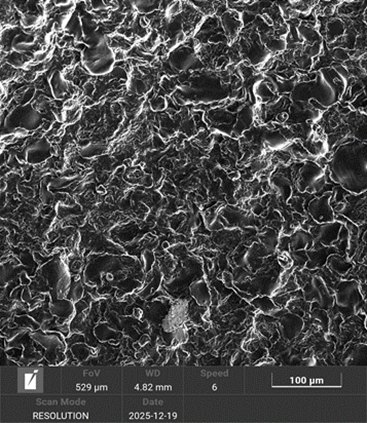
\includegraphics[width=\textwidth]{5.png}
\caption{24 h, low mag}
\end{subfigure}
\\[4pt] % Small vertical space between rows
% Bottom row: High magnification images
\begin{subfigure}{0.32\linewidth}
\centering
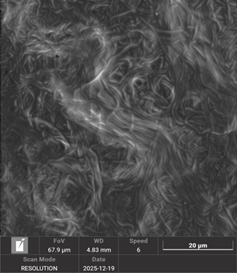
\includegraphics[width=\textwidth]{2.png}
\caption{30 min, high mag}
\end{subfigure}%
\begin{subfigure}{0.32\linewidth}
\centering
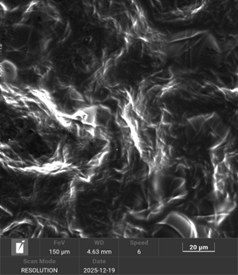
\includegraphics[width=\textwidth]{4.png}
\caption{2 h, high mag}
\end{subfigure}%
\begin{subfigure}{0.32\linewidth}
\centering
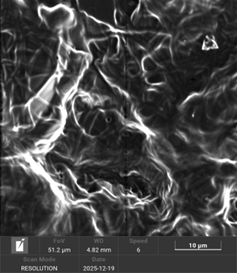
\includegraphics[width=\textwidth]{6.png}
\caption{24 h, high mag}
\end{subfigure}
\caption{SEM images showing morphological evolution of PVA/CA/H3PO4 membranes with increasing doping time.}
\label{fig:sem}
\end{figure}

\section{Fourier Transform Infrared Spectroscopy (FTIR)}
\subsection{Chemical Confirmation of Crosslinking and Acid Incorporation — FTIR-ATR}
FTIR-ATR spectra were recorded for the following samples: uncrosslinked PVA-CA, crosslinked PVA-CA (S0), H\(_3\)PO\(_4\)-doped membrane (S3), and washed membrane. The spectra are presented in Figure 4.2. These four spectra represent the complete chemical history of the membrane fabrication and treatment, with each spectrum corresponding to a chemically unique step in the membrane fabrication and treatment.\cite{36,51}

\subsection{Uncrosslinked PVA-CA Baseline}
The chemical baseline of the uncrosslinked PVA/citric acid precursor is seen in this spectrum. The main feature is a broad, strong band at 3300 cm\(^{-1}\) due to O-H stretching of the abundant hydroxyl groups on the PVA backbone and those in citric acid. The strong C-O stretch from the secondary alcohol on the PVA backbone is seen at 1090 cm\(^{-1}\). Notice that there is no absorption in the 1715 to 1750 cm\(^{-1}\) window, confirming that there are no ester linkages present in this precursor, a useful feature to monitor as we track this reaction.\cite{36, 69}

\subsection{Crosslinking Confirmed — Ester Peak at 1720 cm\(^{-1}\)}
The thermally cured and crosslinked PVA-CA membrane (S0) has an interesting feature in its spectrum. In this spectrum, there is an additional absorption band at 1720 cm\(^{-1}\), not seen in the spectrum of the uncrosslinked membrane. This absorption band is obviously due to the C=O stretching of an ester group and thus offers clear evidence of the condensation reaction between the hydroxyls of PVA and the carboxyls of citric acid.\cite{36,51,96}

This assertion is supported by the predictions of the DFT calculations, as presented in Chapter 5, which predict that the ester formed from the PVA/CA combination should have a C=O stretch at 1720 cm\(^{-1}\), exactly as the experiments show. If we look at the initial free carboxyl group before esterification, the calculation predicts that the scaled C=O stretch should be at 1737 cm\(^{-1}\), and this accounts for the red shift to 1720 cm\(^{-1}\) that we observe, as it must be the result of the decrease in the C=O bond order during esterification.\cite{94}

The continued presence of the O–H stretch at 3300 cm\(^{-1}\) in the crosslinked spectrum also indicates that there are still free hydroxyl groups available. This is consistent with the contact angle results from Section 4.3, where it was shown that the material was still hydrophilic after crosslinking, and also with the DFT prediction that not all of the available hydroxyl groups were utilized for crosslinking at a 10 wt\% citric acid loading.

\subsection{H\(_3\)PO\(_4\) Incorporation}
The fully doped membrane (S3) has two distinct new features: the strong absorption peak at 1000 cm\(^{-1}\), which is due to the P–O stretch of the incorporated phosphate, and the shoulder at 1200 cm\(^{-1}\), which is due to the P=O stretch of the H\(_3\)PO\(_4\) and hydrogen-bonded forms of the phosphoric acid within the polymer structure. The observation of the P–O and P=O bands confirms that the phosphoric acid is present as the molecular form, interacting with the PVA hydroxyl groups via hydrogen bonding, as discussed computationally in Chapter 5.

The much lower baseline transmittance of the doped spectrum is a reflection of the much higher mass loading of the membrane after the acid doping, as confirmed by the gravimetric analysis of the acid uptake as well as the densification of the membrane observed in the SEM images.\cite{52,58}

\subsection{Acid Retention After Water Washing}
The most important information obtained from the FTIR series is the spectrum after the water washing procedure. The P–O peak at 1000 cm\(^{-1}\) remains well identifiable even after the contact with water, though the intensity is lower compared to the doped sample. This indicates that a large amount of the incorporated phosphoric acid remains bound within the network even after the contact with water.\cite{52,55}

This partial retention matches exactly what the DFT hydration stability calculations foretell, as the H\(_3\)PO\(_4\)/water/PVA complex assembly is thermodynamically stable with a free energy of \(-278.0\) kJ/mol. Therefore, the water molecules added to the cooperative binding network enhance the acid’s binding rather than dislodging it from its positions. The O-H region of the broadened peak at 3300 cm\(^{-1}\) increases after washing with water as opposed to the doped spectrum. This aligns with the additional water molecules coordinating with the phosphate-rich network. The four FTIR spectra thus provide a complete chemical history of the fabrication process, with each feature of the spectra directly related to the molecular interactions as described by the DFT calculations of Chapter 5.\cite{21, 55, 94}

\begin{figure}[h!]
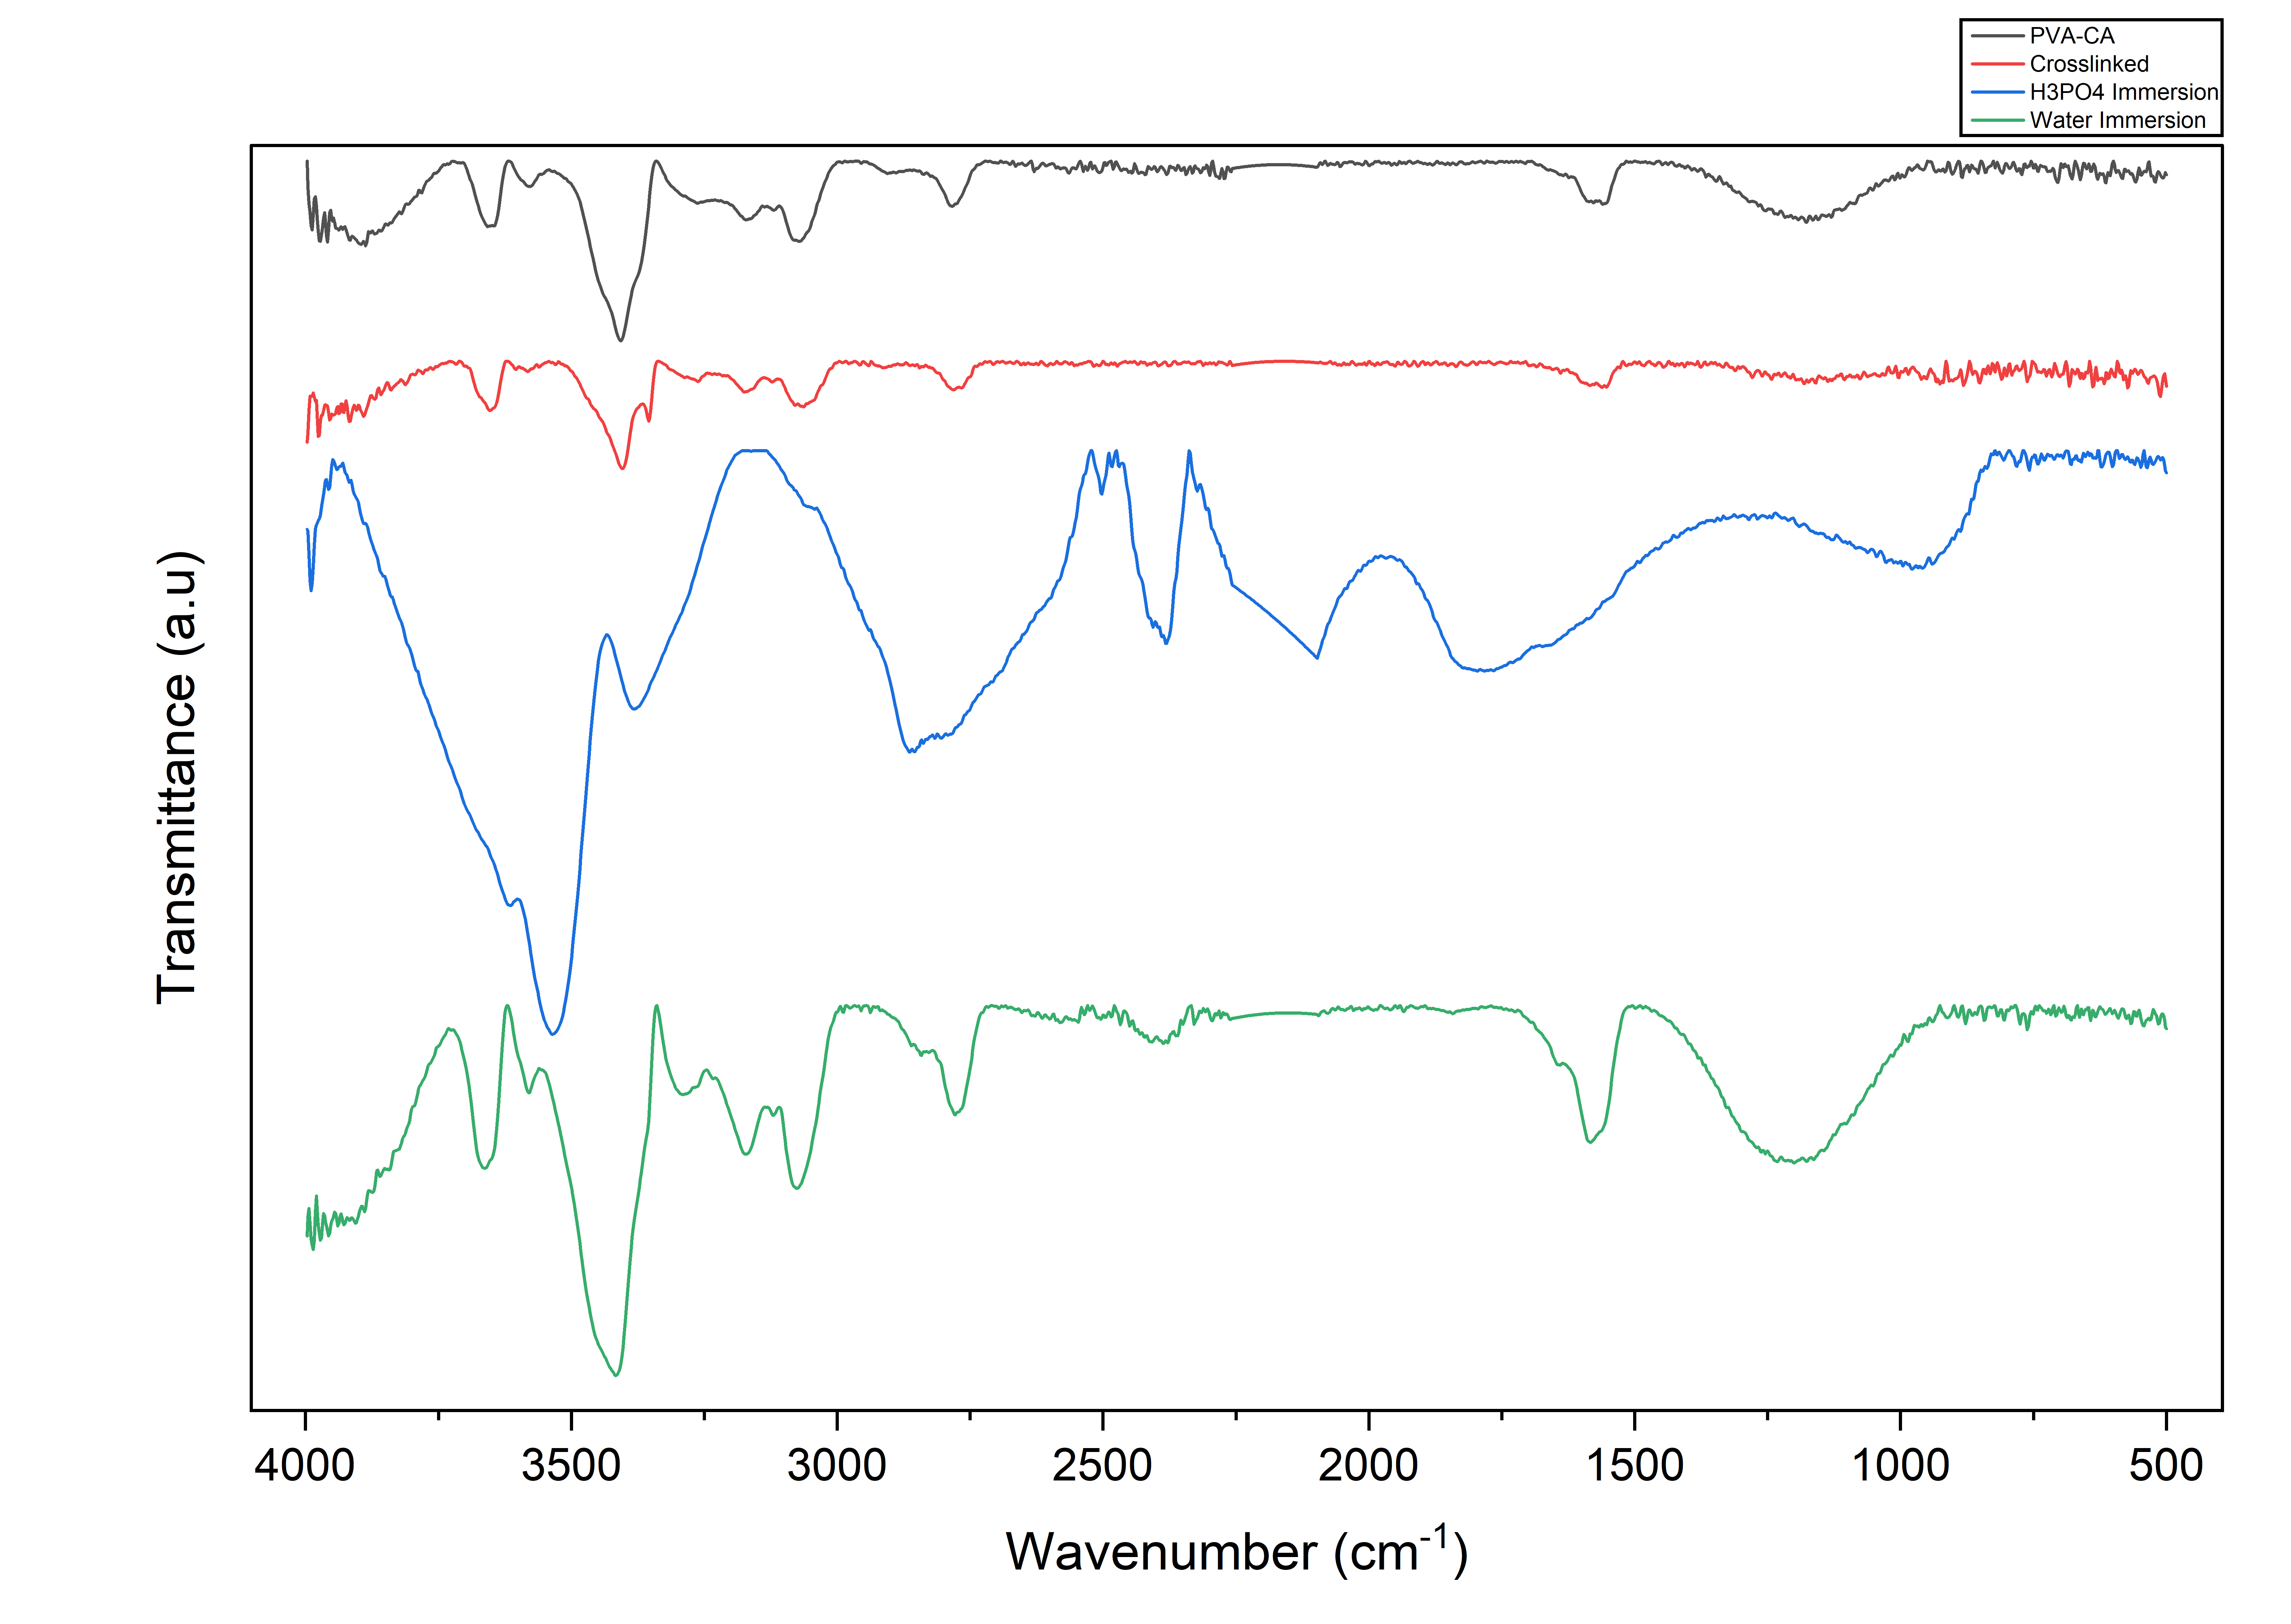
\includegraphics[width=0.9\linewidth]{colored non stacked and better and 600 dpi 4000 to 500.png}
\caption{FTIR of 4 samples}
\centering
\label{fig:ftir-spectra}
\end{figure}

\section{Surface Wettability}
\subsection{Surface Wettability — Contact Angle Analysis}
We determined the static water contact angles of three membrane samples, namely, the uncrosslinked PVA-CA, the crosslinked PVA-CA (S0), and the H$_3$PO$_4$-doped membrane (S3), in order to observe the variation of surface wettability during the fabrication process. The contact angle images are shown in Figure 4.3. Using the contact angles, the work of adhesion ($W_a$) and the surface free energy ($\gamma$) were determined by applying Young’s equation.\cite{71}

\subsection{Uncrosslinked PVA-CA ($\theta = 75.0^\circ$)}
The contact angle of the uncrosslinked membrane is 75.0 degrees, which puts it in the hydrophilic category. The adhesion work of the membrane is 91.7 mJ/m$^2$, while the surface free energy is 45.9 mJ/m$^2$. These values are expected, as published values for PVA films indicate that the dense surface hydroxyl groups create a moderate surface energy that is sufficient to attract water molecules but not sufficient to cause them to spread across the surface of the film.\cite{9, 29} The 75.0-degree contact angle confirms that the uncrosslinked membrane is chemically active, with the hydroxyl groups fully accessible on the surface of the membrane.

\subsection{Crosslinked PVA-CA ($\theta = 83.5^\circ$)}
The contact angle is increased following thermal crosslinking to 83.5$^\circ$, while the work of adhesion decreases to 81.1 mJ/m$^2$, and the surface free energy decreases to 40.5 mJ/m$^2$. The chemical implications of this change are significant because the esterification reaction consumes hydrophilic hydroxyl groups on the surface, replacing them with ester groups which possess lower surface energy. This shift confirms the successful formation of a crosslinked network; the reduction in available –OH groups and the increased packing density of the polymer chains result in a more hydrophobic surface character compared to the uncrosslinked state.\cite{35, 53} This reading is consistent with the FTIR results as seen in Section 4.2.2, where both C=O stretches associated with the ester group and remaining O-H stretches are seen in the crosslinked membrane. This confirms that while crosslinking has significantly altered the surface thermodynamics, some residual hydroxyl groups remain unutilized at 10 wt\% citric acid.

\subsection{H$_3$PO$_4$-Doped Membrane ($\theta = 50.6^\circ$)}
The most significant change in this series is seen after doping with phosphoric acid. The contact angle is reduced significantly to 50.6$^\circ$. The reduction is 24.4$^\circ$ from the baseline of the uncrosslinked membranes and 32.9$^\circ$ from that of the crosslinked membrane. Since $\theta$ is 50.6$^\circ$, it is clear that this membrane is strongly hydrophilic with a work of adhesion equal to 119.2 mJ/m$^2$ and a surface free energy close to 59.6 mJ/m$^2$. This is due to its molecular origins. The addition of H$_3$PO$_4$ includes highly hygroscopic phosphate groups that strongly attract water molecules through hydrogen bonding as well as the cooperative binding network as calculated by DFT, where multiple H$_3$PO$_4$ molecules simultaneously bind to the neighboring PVA hydroxyl groups with a total binding energy of 203.0 kJ/mol. This is a densely populated surface with high affinity for water molecules, which strongly attract sessile drops, resulting in significantly lower contact angles.\cite{21, 55} As the drop shape flattens toward 50.6$^\circ$, the macroscopic-level takeaway is that this surface thermodynamics is consistent with the Grotthuss proton relay network at the molecular level. The same hydrogen bonding network that enables the rapid hopping of protons within the membrane also enables this surface to strongly attract water molecules. This is just one of the consistencies that the combined work of this dissertation highlights.\cite{21, 55, 71}


\begin{figure}[htbp]
    \centering
    \begin{subfigure}{0.32\linewidth}
        \centering
        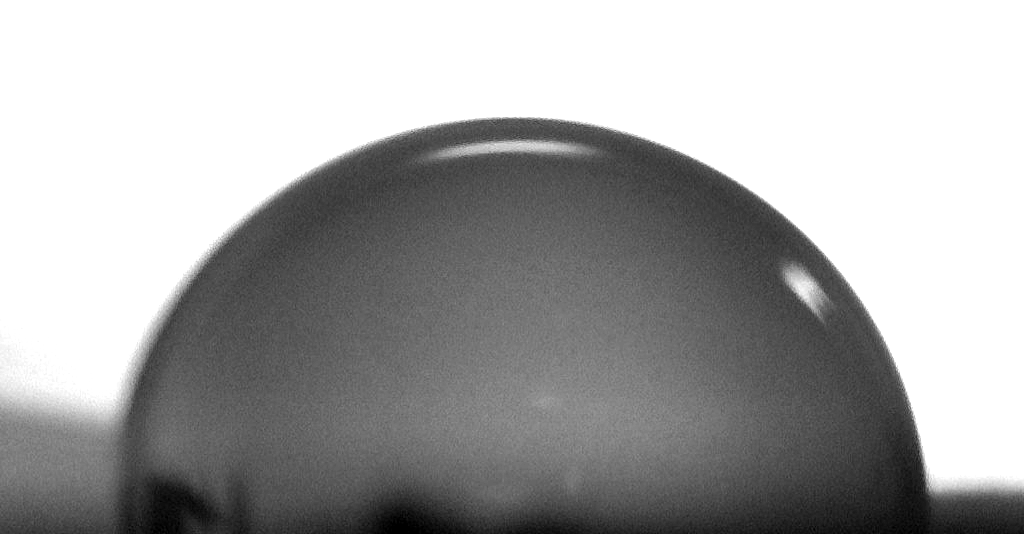
\includegraphics[width=\textwidth]{PVA-Citric acid Shahid2.png}
        \caption{PVA/CA (Uncrosslinked) $\theta \approx 75.0^\circ$}
        \label{fig:ca_uncrosslinked}
    \end{subfigure}
    \hfill
    \begin{subfigure}{0.32\linewidth}
        \centering
        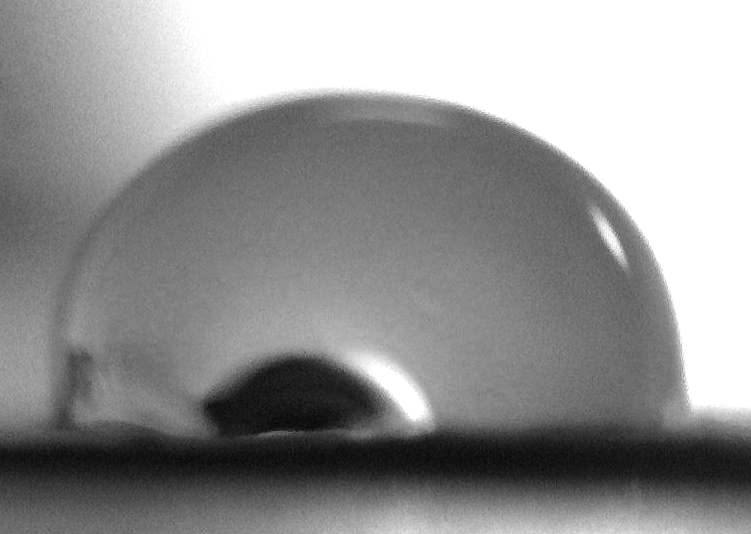
\includegraphics[width=\textwidth]{PVA-citric acid cross linked2.png}
        \caption{Crosslinked PVA/CA $\theta \approx 83.5^\circ$}
        \label{fig:ca_crosslinked}
    \end{subfigure}
    \hfill
    \begin{subfigure}{0.32\linewidth}
        \centering
        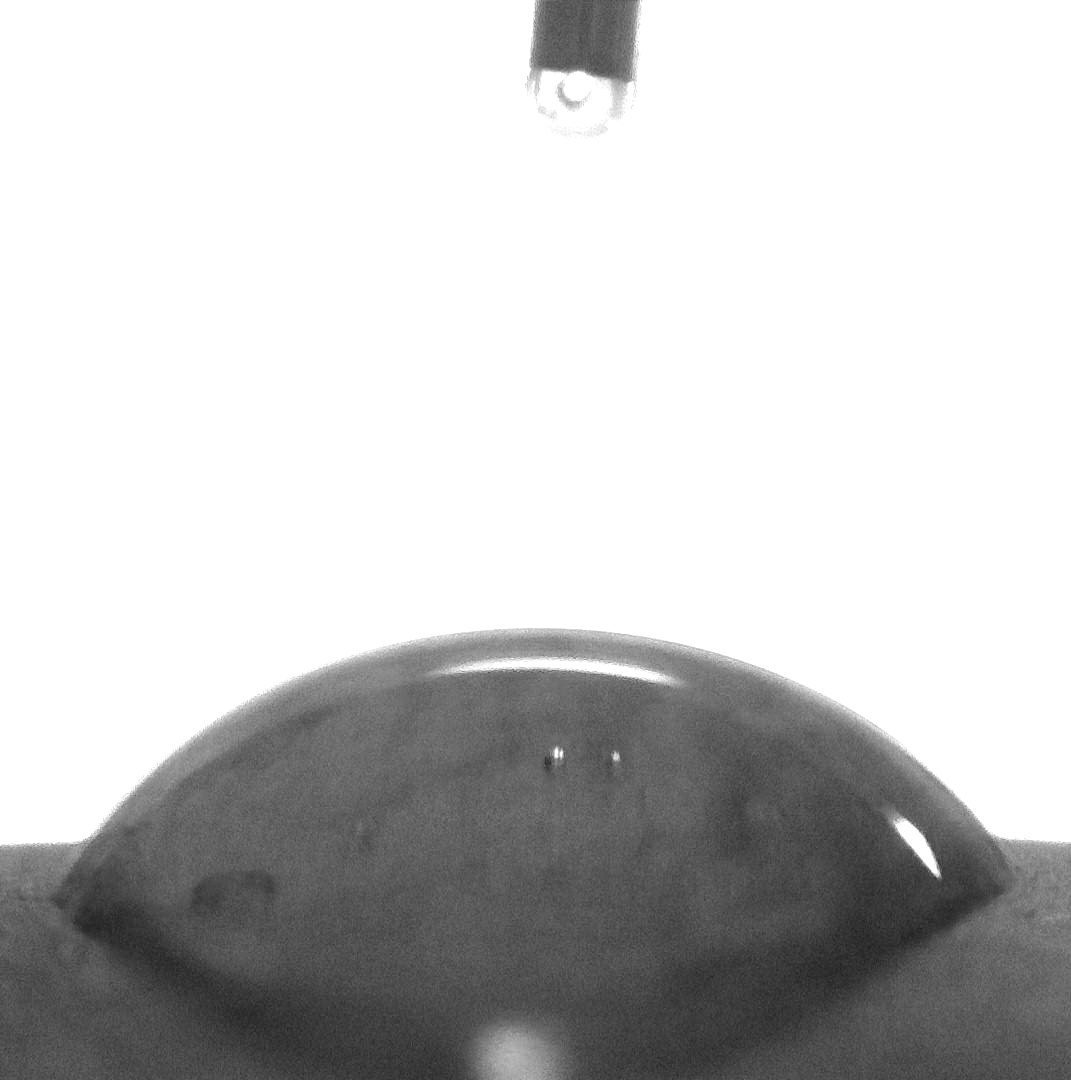
\includegraphics[width=\textwidth]{impregranted.png}
        \caption{H$_3$PO$_4$-Doped (30\%) $\theta \approx 50.6^\circ$}
        \label{fig:ca_doped}
    \end{subfigure}
    \caption{Wettability transition of the membrane series. The contact angle initially increases from (a) to (b) due to the consumption of hydroxyl groups during thermal crosslinking, followed by a significant decrease in (c) after $H_3PO_4$ doping, indicating enhanced hydrophilicity.}
    \label{fig:contact_angle_evolution}
\end{figure}

\section{Conductivity} [THIS SECTION IS WRITTEN AS AN EXAMPLE. THIS WILL BE EITHER REWRITTEN OR EDITED. SKIP THIS READ]
\subsection{Proton Conductivity and Electrochemical Performance}
% Placeholder: The following content is from your document, but you mentioned missing sections. We'll keep what's there.
Electrochemical impedance spectroscopy was used to measure the proton conductivity of each membrane sample and to extract the proton transport activation energy from the temperature dependence of conductivity. The results provide the key experimental benchmark against which the DFT proton transfer barriers computed in Chapter 5 are compared.
\subsection{EIS Measurements and Equivalent Circuit Fitting}
Nyquist plots were recorded for all four samples (S0–S3) at 25\(^\circ\)C over the frequency range 0.01 Hz – 1 MHz. The plots show a compressed semicircle at high frequencies corresponding to the bulk membrane response, with a Warburg diffusion tail at low frequencies. All spectra were fitted using the equivalent circuit described in Section 3.7.1, comprising a series resistance (\(R_\infty\)), a constant phase element (CPE) in parallel with a charge-transfer resistance (\(R_{ct}\)), and a finite-length Warburg element.\cite{65,66}

The quality of fit was assessed by the chi-squared value (\(\chi^2 < 10^{-3}\) for all samples) and by visual inspection of the superimposed measured and fitted Nyquist curves. The bulk membrane resistance \(R_b\) was taken as the high-frequency real-axis intercept of the fitted semicircle. Membrane thickness was measured by digital micrometer at five positions across each sample and the average value used in the conductivity calculation.\cite{65,67}

\begin{figure}[h!]
\centering
\fbox{\parbox{0.9\textwidth}{\centering FIGURE 4.4 — INSERT HERE \\
Nyquist plots for samples S0–S3 at 25\(^\circ\)C. Frequency range 0.01 Hz – 1 MHz. Points: experimental data. Lines: equivalent circuit fits. Inset: equivalent circuit model showing \(R_\infty\), CPE, \(R_{ct}\), and Warburg element. Table of fitted parameters (\(R_\infty\), \(R_b\), CPE exponent) for each sample.}}
\caption{Nyquist plots and equivalent circuit fits for samples S0–S3.}
\label{fig:nyquist}
\end{figure}

\subsection{Conductivity Progression Across S0–S3}
The proton conductivity values calculated from the fitted bulk resistance values are: S0 (undoped) = 1 mS/cm, S1 (30 min) = 10 mS/cm, S2 (2h) = 22 mS/cm, S3 (24h) = 35 mS/cm. The progressive increase across the doping series confirms that phosphoric acid loading is the primary driver of proton conductivity in this membrane system, consistent with the established role of H\(_3\)PO\(_4\) as a Grotthuss proton conductor.\cite{21,55,56}

The conductivity of 35 mS/cm achieved by S3 is competitive with non-fluorinated alternative membranes reported in the literature and falls within a factor of approximately three of the conductivity of Nafion 117 under ambient conditions (approximately 90–100 mS/cm at full hydration).\cite{5,6} Importantly, PVA/CA/H\(_3\)PO\(_4\) achieves this conductivity without fluorinated chemistry and with the potential for improved performance above 80\(^\circ\)C — conditions under which Nafion conductivity degrades due to dehydration.\cite{3,4,5}

\begin{figure}[h!]
\centering
\fbox{\parbox{0.9\textwidth}{\centering FIGURE 4.5 — INSERT HERE \\
Proton conductivity values for samples S0–S3 at 25\(^\circ\)C plotted as a bar chart. Error bars represent \(\pm\) standard deviation from triplicate measurements. Nafion 117 literature value shown as a dashed reference line. Inset: conductivity values tabulated with membrane thickness and bulk resistance.}}
\caption{Proton conductivity progression across doping times.}
\label{fig:conductivity-bars}
\end{figure}

\subsection{Arrhenius Analysis: Activation Energy Across the Doping Series}
Temperature-dependent conductivity measurements were performed between 25\(^\circ\)C and 80\(^\circ\)C for each sample. The Arrhenius plots of \(\ln(\sigma)\) versus \(1/T\) are shown in Figure 4.6. All plots show excellent linearity (\(R^2 > 0.99\)), confirming thermally activated proton transport in all samples. The activation energies extracted from the slopes are: S1 = 20.9 kJ/mol, S2 = 14.5 kJ/mol, S3 = 10.2 kJ/mol.\cite{65,66}

The systematic decrease in \(E_a\) with increasing doping time is one of the most important experimental results of this study, and it has a direct molecular interpretation provided by the DFT calculations in Chapter 5. As doping time increases, more H\(_3\)PO\(_4\) molecules are incorporated and the cooperative hydrogen bond network described in Section 5.1.4 grows denser. Each additional acid molecule that enters the cooperative network finds a more polarised, more activated binding environment — creating shorter hydrogen bonds with lower per-hop transfer barriers. The DFT CalcNew3 barrier of 19.5 kJ/mol falls within the experimental activation energy range of 10.2–20.9 kJ/mol, providing quantitative validation of the computational model.\cite{21,72,73}

\begin{figure}[h!]
\centering
\fbox{\parbox{0.9\textwidth}{\centering FIGURE 4.6 — INSERT HERE \\
Arrhenius plots of \(\ln(\sigma)\) versus \(1000/T\) for samples S1, S2, and S3 over the temperature range 25–80\(^\circ\)C. Points: experimental data. Lines: linear fits. Activation energies (\(E_a\)) extracted from slopes labelled for each sample. \(R^2\) values shown.}}
\caption{Arrhenius plots and activation energies for doped membranes.}
\label{fig:arrhenius}
\end{figure}

\subsection{Non-Linear Conductivity Enhancement with Doping Time}
The conductivity increase from S0 to S3 is clearly non-linear. The step from S0 to S1 (30 min doping) produces a 10-fold increase in conductivity (1 → 10 mS/cm), the step from S1 to S2 produces a further 2.2-fold increase (10 → 22 mS/cm), and the step from S2 to S3 produces only a 1.6-fold increase (22 → 35 mS/cm). A simple linear acid-loading model — in which each H\(_3\)PO\(_4\) molecule contributes equally and independently to conductivity — would predict proportionally equal gains at each step. The observed superlinear enhancement in the early doping stages and the levelling off at extended doping times cannot be explained by acid quantity alone.\cite{57,58}

The DFT cooperative binding analysis in Section 5.1.4 provides a quantitative molecular explanation. The first H\(_3\)PO\(_4\) molecules to enter the membrane at 30 minutes occupy the strongest single-site binding positions (\(-78.1\) kJ/mol), forming isolated proton relay contacts. As doping continues, subsequent molecules bind cooperatively alongside those already present, achieving combined binding energies of \(-203.0\) kJ/mol for two-molecule assemblies — a 30\% enhancement per molecule relative to the isolated case. These cooperative-binding molecules form stronger relay chains with shorter H···O contacts and lower effective transfer barriers, producing the superlinear conductivity gain observed experimentally.\cite{21,55}

The levelling off at extended doping times reflects saturation of the cooperative binding sites: once the available hydroxyl groups are occupied, additional acid molecules can only occupy less favourable positions with diminishing conductivity returns. This picture is fully consistent with the two-population acid retention model derived from the DFT desorption PES in Section 5.3.3.

\subsection{Comparison with Nafion 117 and Published Literature Values}
The conductivity of S3 (35 mS/cm at 25\(^\circ\)C, ambient humidity) is compared with published values for Nafion 117 and selected alternative membranes in Table 4.1. Nafion 117 under fully humidified conditions at 25\(^\circ\)C delivers approximately 90–100 mS/cm.\cite{5,6} The PVA/CA/H\(_3\)PO\(_4\) membrane achieves roughly one-third of the Nafion conductivity under comparable measurement conditions, which represents a meaningful performance level for a non-fluorinated alternative produced without expensive raw materials or complex synthesis.

Among published PVA-based membranes, the conductivity of 35 mS/cm is competitive with values reported for PVA/H\(_3\)PO\(_4\) blends (10–40 mS/cm) and PVA/sulfosuccinic acid membranes (20–30 mS/cm).\cite{21,57,58} The electrospun nanofiber architecture, which maximises the accessible surface area for acid uptake, is likely responsible for the performance at the upper end of this range for the S3 sample.\cite{12,13,14}

\begin{table}[h!]
\centering
\caption{Comparison of proton conductivity of S3 membrane with literature values.}
\label{tab:conductivity-comparison}
\begin{tabular}{l l c c c}
\hline
Material & Doping/Treatment & \(\sigma\) (mS/cm) & T (°C) & Reference \\
\hline
Nafion 117 & Fully hydrated & 90–100 & 25 & \cite{5,6} \\
PVA/H\(_3\)PO\(_4\) blend & Various & 10–40 & 25 & \cite{57,58} \\
PVA/sulfosuccinic acid & Crosslinked & 20–30 & 25 & \cite{113} \\
This work — S3 & 24h doping & 35 & 25 & — \\
\hline
\end{tabular}
\end{table}

\chapter{Computational Results and Discussion}

This chapter presents 31 density functional theory calculations, all carried out at the B3LYP-D3BJ/6-31G* level with the ORCA 6.1.1 program.[77–79] These calculations are further complemented by molecular dynamics (MD) simulations performed with LAMMPS and macroscopic device modeling conducted with COMSOL Multiphysics. 
\section{Thermodynamics}
\subsection{Thermodynamics of Crosslinking and Acid Binding}
First, each molecule was optimized on its own, without any partners. This generates the reference energy used for all binding and reaction energy calculations, as well as ensuring that the method being used correctly represents each molecule prior to any interactions being introduced.

\subsubsection{Baseline Molecular Geometries of Isolated Components}

\textbf{Phosphoric Acid (H\(_3\)PO\(_4\))}
The optimized structure of the H\(_3\)PO\(_4\) molecule is illustrated in Figure 5.1(a). It can be seen that the phosphorus atom is at the center of the molecule and is bonded to one non-protonated oxygen by a P=O double bond and to three hydroxyl groups (P–OH) in a tetrahedral shape. The calculated bond length of the P=O bond is found to be 1.479 Å, which is close to the bond length of 1.481 Å found in the crystal structure of the compound with only a difference of 0.002 Å or 0.1\%.\cite{76}
The three P-OH bonds are found at approximately 1.60 Å, somewhat longer than a standard P=O bond as would be expected for single bonds. The O-H bonds are found at approximately 0.97 Å, suggesting a moderately polar O-H group. The CHELPG calculation\cite{99} indicates that the phosphorus atom has a +2.1 e charge, while the non-protonated oxygen has a -0.9 e charge, demonstrating just how polar this P=O bond is. These values collectively indicate that H\(_3\)PO\(_4\) is a very potent proton donor, with its P-O-H groups being able to engage in hydrogen bonding with nearby acceptors, thereby accounting for its ability to function as a proton conductor within the PVA membrane.

\textbf{PVA Monomer — Isopropanol}
Isopropanol, with the structure CH\(_3\)CH(OH)CH\(_3\), is the proxy used for the PVA repeat unit in Figure 5.1(b). The reason we cannot deal with the entire PVA chain at this level of detail is that it is much too long, so we use a simpler molecule that has the key feature of a secondary alcohol group attached to a carbon backbone.\cite{18,19}

The length of the O–H bond is 0.970 Å, while the length of the C–O bond is 1.430 Å, which is what we expect for a secondary alcohol group. The lengths of the C–C backbone bonds are around 1.525 Å. The CHELPG charge on the oxygen of the hydroxyl group is -0.72e,\cite{99} showing that this is a highly electron-rich center, a good hydrogen bond acceptor. When the H\(_3\)PO\(_4\) enters the picture, the hydrogen from the phosphoric acid attacks this oxygen, which has a high negative charge, as we see from the above values, which helps explain the high binding energy that we saw in Section 5.1.3.

\textbf{Citric Acid}
Citric acid contains three carboxyl groups with three C=O bonds connected to a central hydroxyl group. The C=O bond lengths range from 1.208 to 1.215 Å, while the C-OH bond lengths range from 1.308 to 1.319 Å. The C-O bond lengths of the carboxyl group are slightly less than the standard C-O bond due to the extension of the electron density of the two oxygen atoms. The C-O bond of the hydroxyl group measures 1.415 Å, a typical bond of a secondary alcohol.

Table 5.1 presents the computed bond lengths of the molecule, along with the experimental values used as references. The differences between them are all less than 0.014 Å, thus verifying the accuracy of the B3LYP-D3BJ/6-31G* method used in this research.\cite{76}

\begin{table}[h!]
\centering
\caption{Baseline geometries — computed vs reference values.}
\label{tab:baseline-geometries}
\begin{tabular}{l l c c c}
\toprule
Parameter & Molecule & DFT (Å or °) & Reference (Å or °) & Deviation \\
\midrule
P=O bond & H\(_3\)PO\(_4\) & 1.479 & 1.481 & 0.002 (0.1\%) \\
P–OH bond & H\(_3\)PO\(_4\) & 1.594–1.614 & 1.580–1.610 & $<0.014$ \\
O–H bond & H\(_3\)PO\(_4\) & 0.970–0.973 & 0.967–0.980 & $<0.010$ \\
O–P–O angle (°) & H\(_3\)PO\(_4\) & 103–118 & 101–116 & $<2^\circ$ \\
O–H bond & Isopropanol & 0.970 & 0.961–0.975 & $<0.010$ \\
C–O bond & Isopropanol & 1.430 & 1.425–1.440 & $<0.010$ \\
C–C bond & Isopropanol & 1.525 & 1.522–1.534 & $<0.009$ \\
C=O bond & Citric acid & 1.208–1.215 & 1.200–1.220 & $<0.012$ \\
C–OH bond & Citric acid & 1.308–1.319 & 1.300–1.320 & $<0.011$ \\
Central C–OH & Citric acid & 1.415 & 1.410–1.420 & $<0.005$ \\
\bottomrule
\end{tabular}
\end{table}

\begin{figure}[h!]
\centering
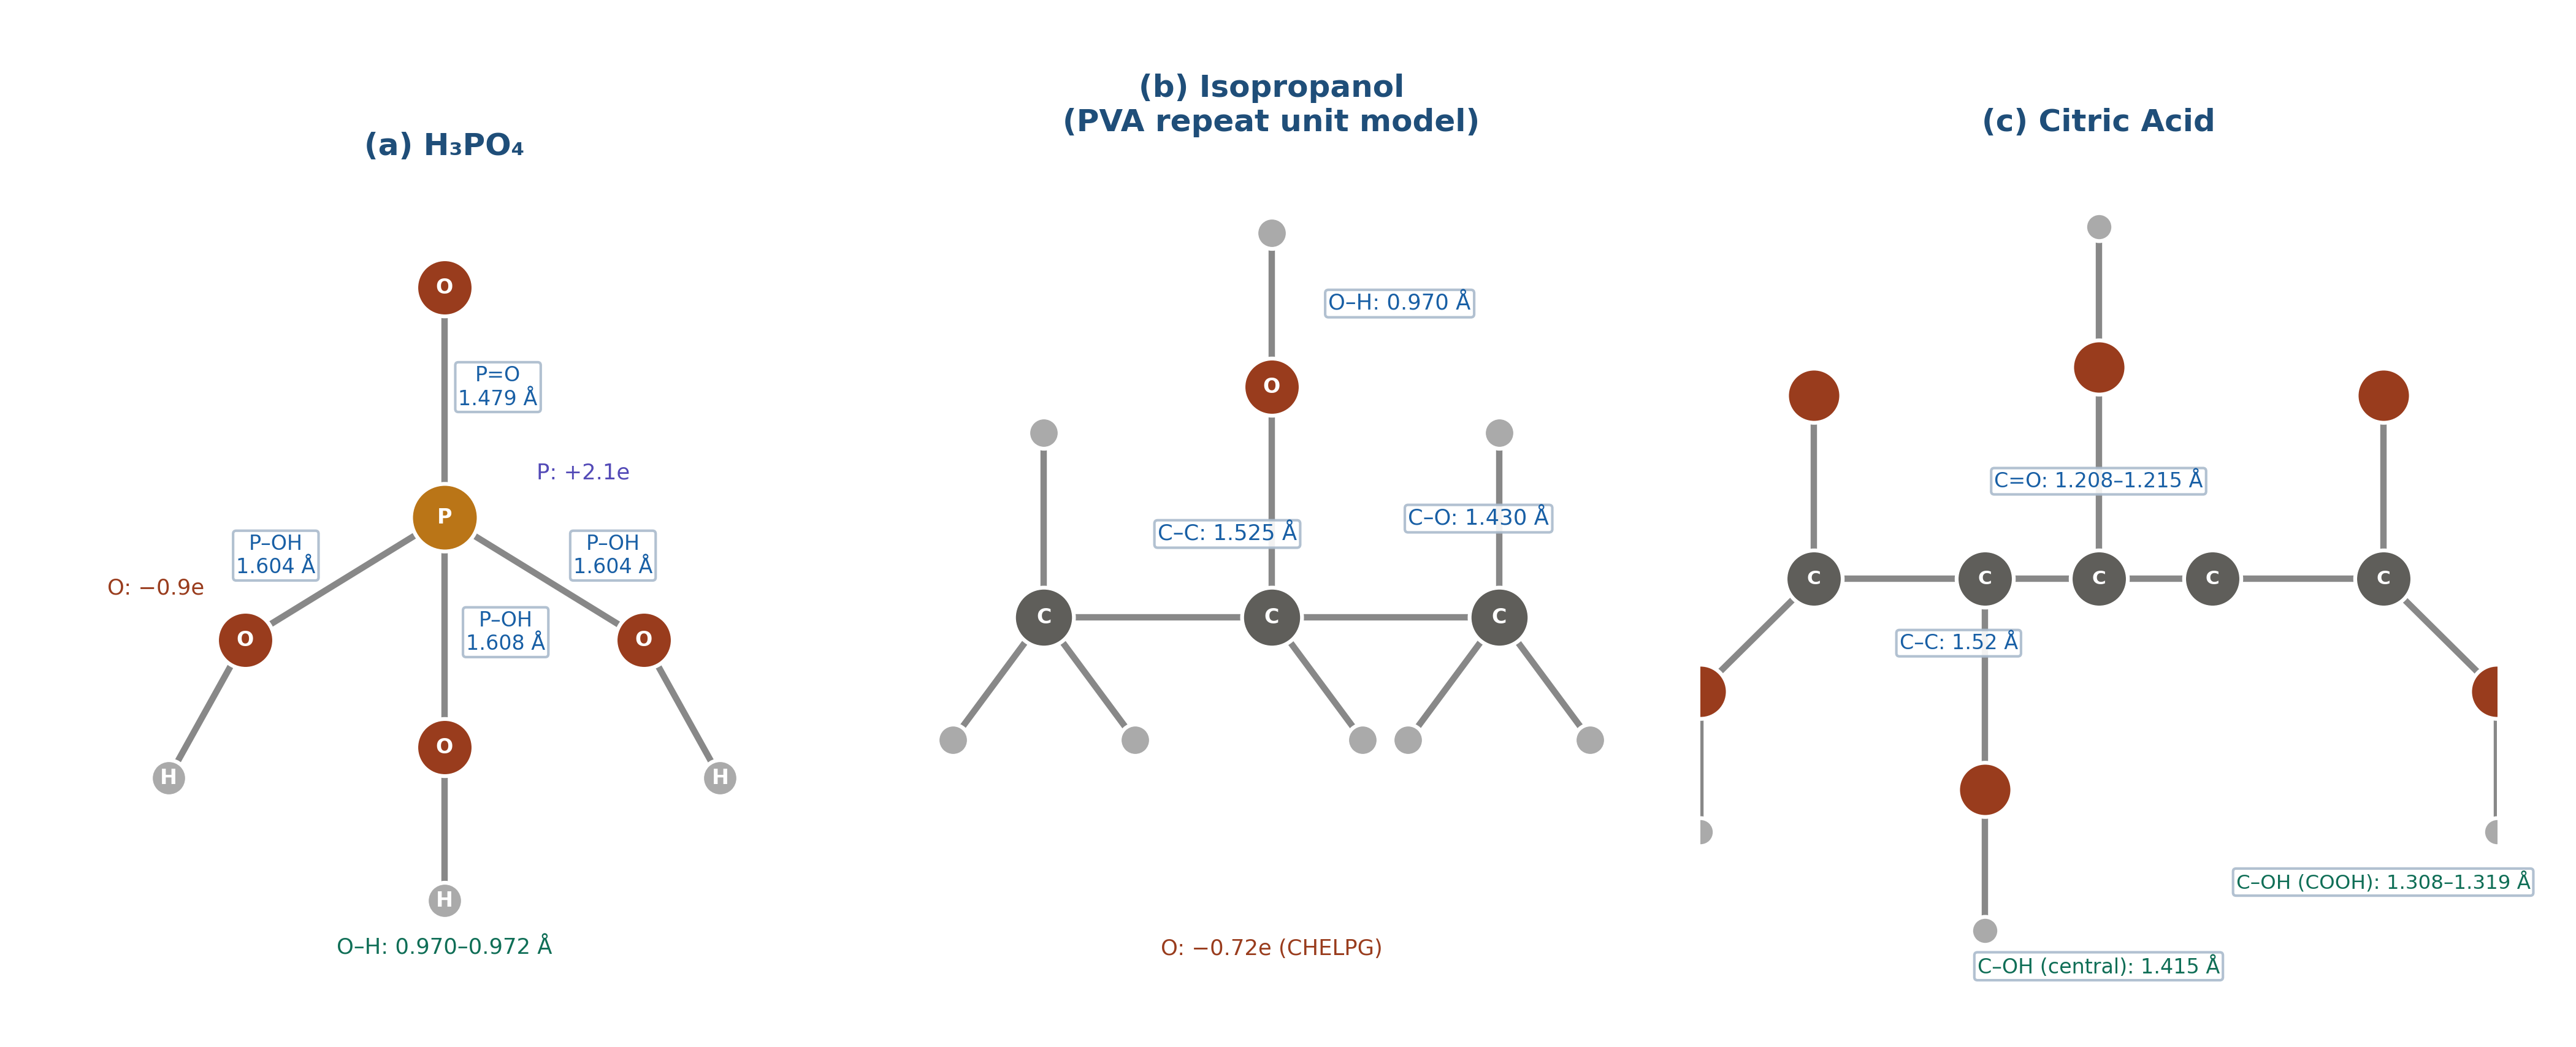
\includegraphics[width=0.8\linewidth]{Fig5_1_baseline_geometries.png}
\caption{Baseline geometries}
\label{fig:isolated-geometries}
\end{figure}

\subsubsection{Esterification Energy and Crosslink Formation}

\textbf{Reaction Energy and Thermodynamic Spontaneity}
In addition, during the fabrication of membranes, when citric acid and PVA are subjected to heat, an esterification reaction occurs. The hydroxyl group in PVA reacts with the carboxyl group in citric acid, forming an ester compound with the release of one mole of water. The reaction energy calculated using DFT is -12.4 kJ/mol, showing that this reaction is thermodynamically spontaneous since more energy is released when the product is formed.\cite{53,96}
The small energy change is consistent with this chemistry because esterification is reversible under acidic or basic conditions. The crosslinked membrane is stable under mild aqueous conditions, as required in fuel cells, but would not be stable under acidic or basic conditions, as is consistent with simple ester chemistry. The reaction is also consistent with experimental conditions because 150\(^\circ\)C is sufficient to induce crosslinking without a catalyst.\cite{35,50}

\textbf{Optimised Ester Product Geometry}
The optimized geometry of the ester product is given in Figure 5.2. The length of the C=O bond in the ester product is 1.2281 Å, while the length of the C-O single bond in the product is 1.3246 Å. These values correspond to the conjugated ester group, in which the electron density from the C-O bond is delocalized into the C=O, causing the C-O single bond to be slightly shorter than the typical 1.43 Å for an alcohol C-O bond. There are two distinct ester bonds in the CalcNew2 fully crosslinked structure, both of length 1.2223 Å and 1.2323 Å, differing slightly due to the differing local environment at the two ends of the citric acid bridge.

\textbf{DFT-Predicted IR Frequency and Experimental Validation}
The free carboxyl C=O stretch of the citric acid has a scaled DFT frequency of 1737 cm\(^{-1}\). The frequency of this vibration is lowered by 17 cm\(^{-1}\) when the carboxyl is esterified, as the C=O bond order is lower in the ester than in the carboxyl, giving a frequency of 1720 cm\(^{-1}\). This is exactly the same as the FTIR-ATR peak discussed in Section 4.2.2. The DFT results provide a rationale for the position of this peak, showing that they are observing the same process at the same energy level.\cite{36, 51, 94}

\begin{figure}[h!]
\centering
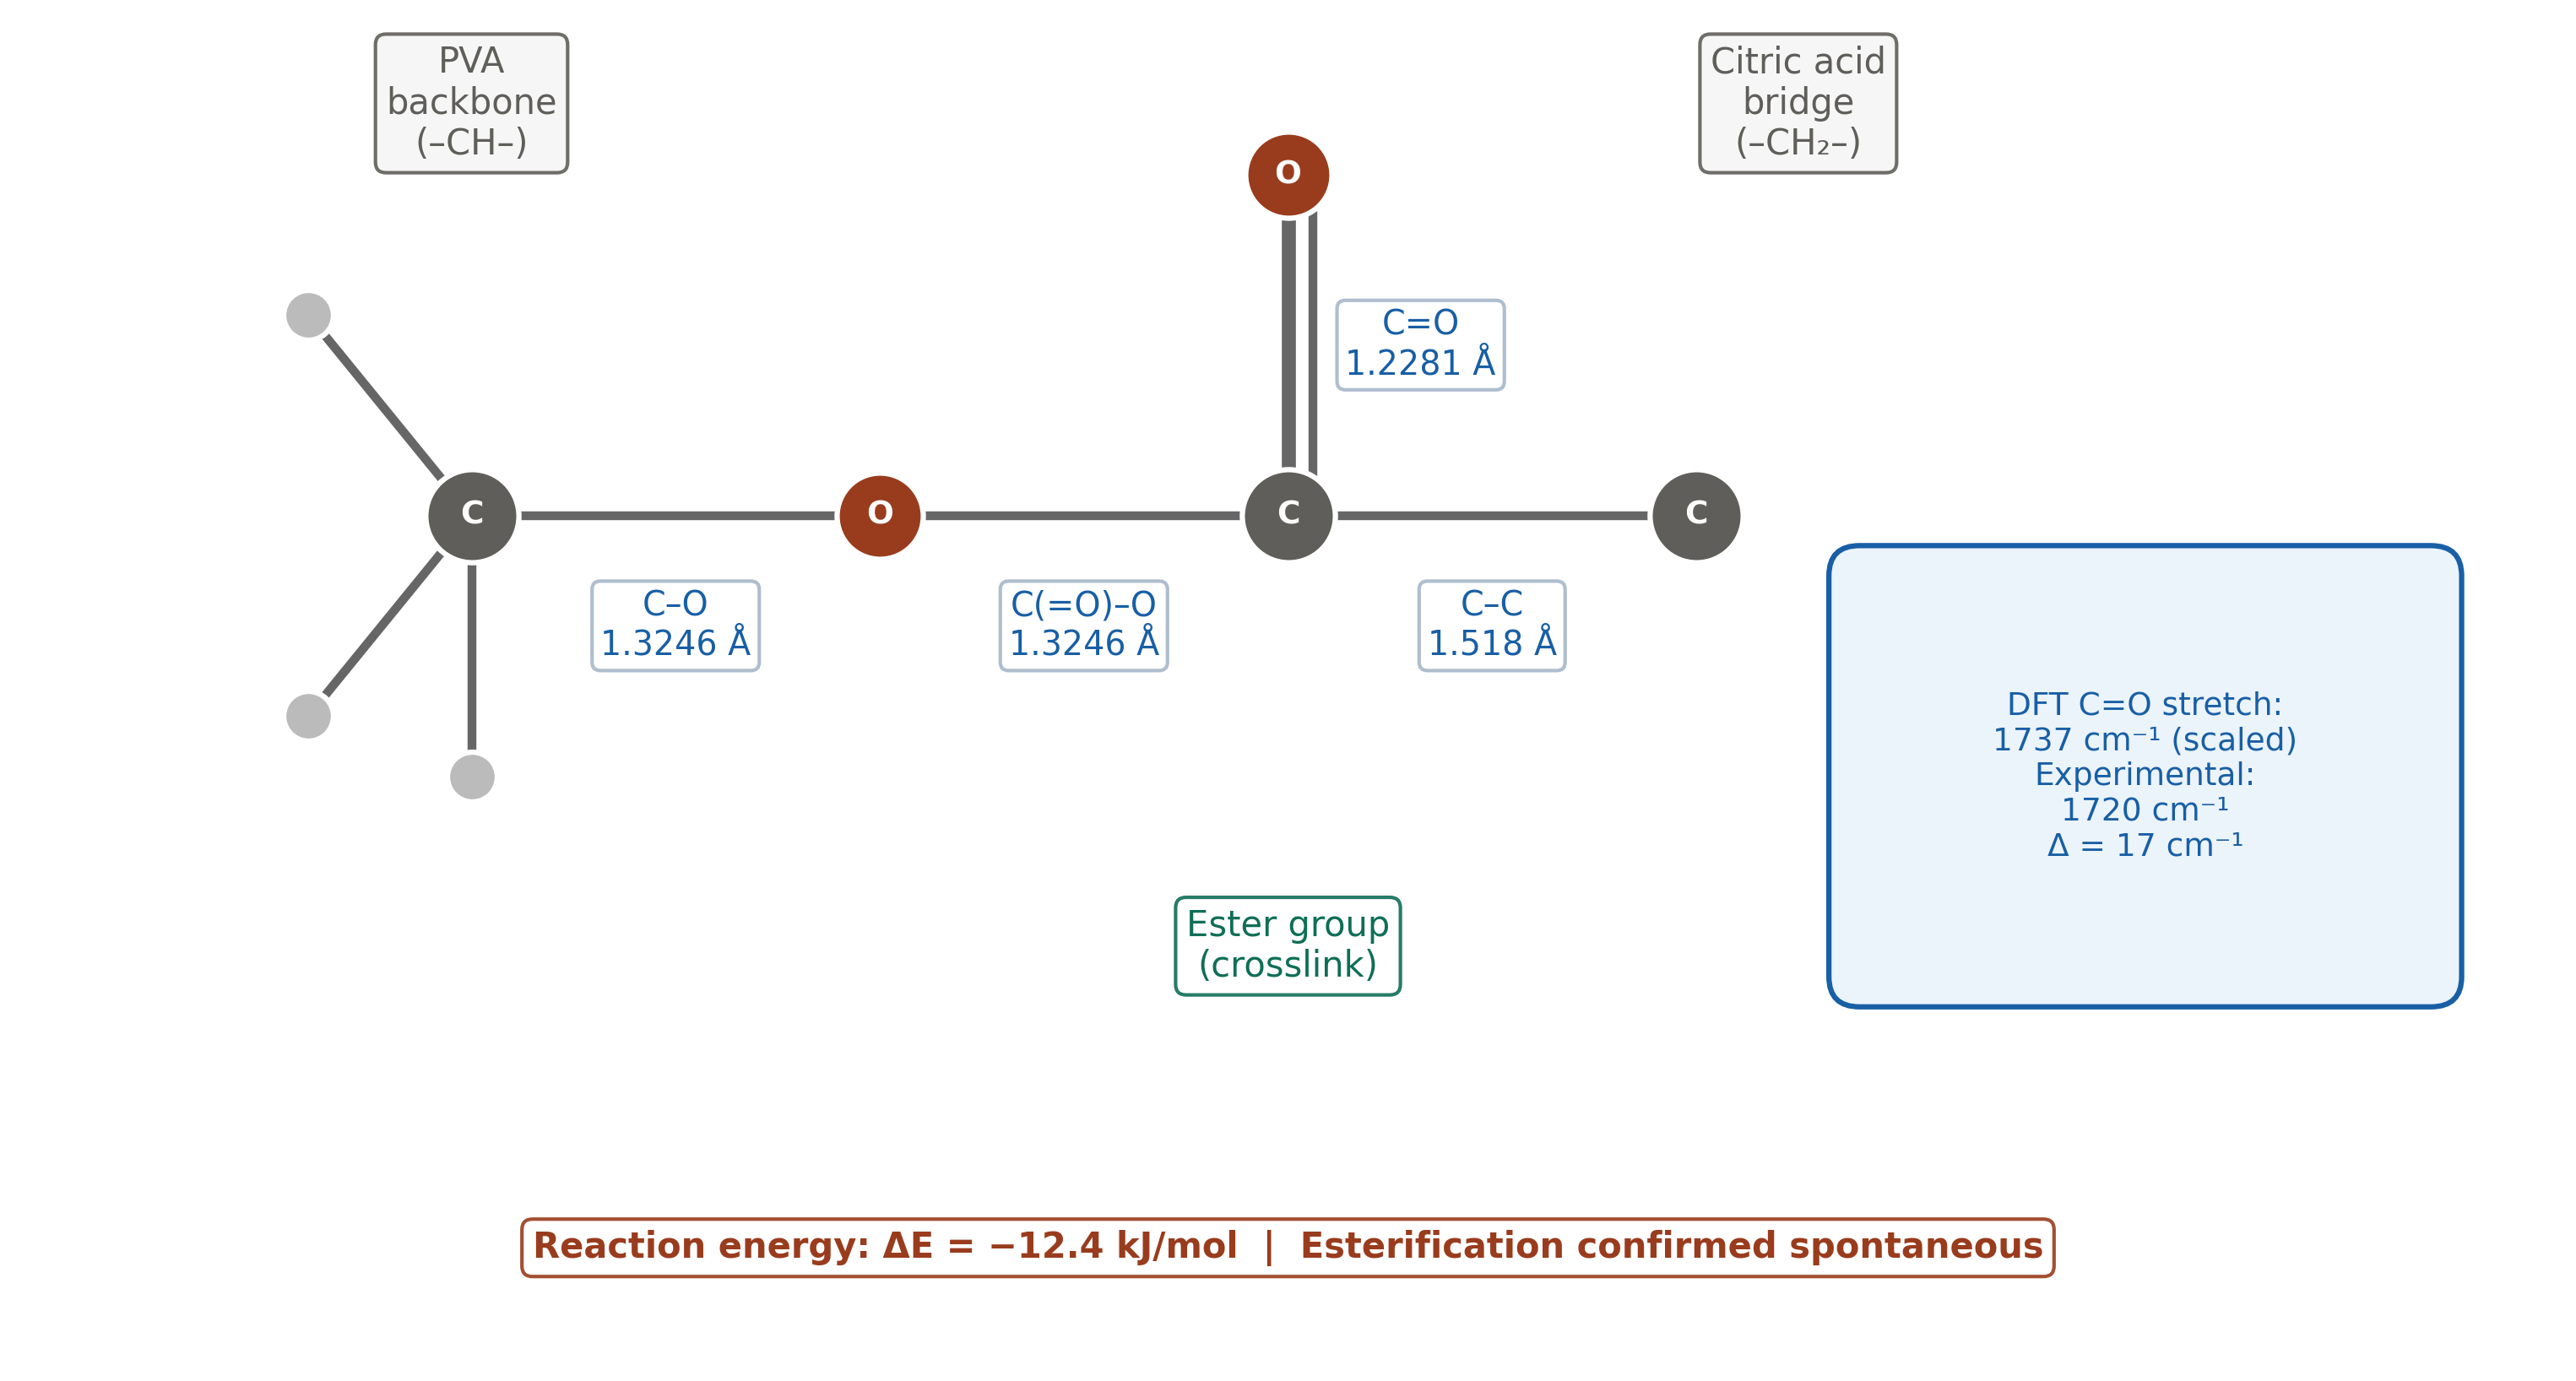
\includegraphics[width=0.8\linewidth]{Fig5_2_ester_geometry.png}
\caption{Optimised ester product geometry and DFT-predicted IR frequency.}
\label{fig:ester-product}
\end{figure}

\subsubsection{H\(_3\)PO\(_4\) Binding to PVA — Single-Site Interaction}

\textbf{Hydrogen Bond Geometry}
In other words, when phosphoric acid (H\(_3\)PO\(_4\)) reacts with the hydroxyl (-OH) of polyvinyl alcohol (PVA), one hydrogen bond is created. In this hydrogen bond, the P-OH donates and the oxygen of PVA accepts. The stable geometry of this hydrogen bond is given below in Table 5.2.

The bond length of hydrogen and oxygen is 1.707 Å. This bond length is solidly placed in the region of strong hydrogen bonds. According to Jeffrey’s rule of thumb, strong O-H···O bonds should be shorter than 1.8 Å. In contrast,\cite{97} hydrogen bond lengths for liquid water molecules measure 1.97 Å. The hydrogen bond between PVA and H\(_3\)PO\(_4\) is shorter and stronger. As the hydrogen bond is created, the O-H bond lengthens from 0.970 Å for H\(_3\)PO\(_4\) to 0.989 Å for the hydrogen bond. This is an increase of 0.019 Å. This increase happens because of electron density being donated from the oxygen of PVA into the O-H antibonding orbitals.\cite{97,98} This same process, continued further, is what happens during the proton transfer event described in Section 5.2.

\begin{table}[h!]
\centering
\caption{Hydrogen bond geometry — PVA–H\(_3\)PO\(_4\) binary complex.}
\label{tab:hbond-geometry}
\begin{tabular}{l c l}
\toprule
Parameter & Value & Interpretation \\
\midrule
H···O(acceptor) distance (Å) & 1.707 & Strong H-bond ($<1.8$ Å) \\
O···O separation (Å) & 2.653 & Consistent with strong H-bond (2.5–2.8 Å range) \\
Donor O–H free H\(_3\)PO\(_4\) (Å) & 0.970 & Reference \\
Donor O–H in complex (Å) & 0.989 & +0.019 Å elongation \\
CHELPG charge on H free (e) & +0.432 & Free H\(_3\)PO\(_4\) \\
CHELPG charge on H (complex) & $+0.389\,e$ & $-0.043\,e$ transfer to acceptor \\
P: CHELPG charge & $+2.1\,e$ & High polarity of P–O bonds \\
O(acceptor): CHELPG charge & $-0.72\,e$ & Strong acceptor character of PVA–O \\
Binding energy & $-78.1$ kJ/mol & Upper range of strong H-bonds \\
\bottomrule
\end{tabular}
\end{table}

\textbf{Binding Energy}
The binding energy here is given by: \(\Delta E_{\text{bind}} = -78.1\) kJ/mol.
This value should be noted as quite high when considering non-covalent interactions. For example, the hydrogen bonds in water are typically on the order of 20-25 kJ/mol, while the strong hydrogen bonds in carboxylic acid dimers are on the order of 50-60 kJ/mol.\cite{97} This value of 78.1 kJ/mol reflects the combination of a strong acid in H\(_3\)PO\(_4\) and the strong accepting ability of the hydroxyl oxygen of PVA. In other words, the phosphoric acid binds quite strongly to the PVA network, and this strong binding ability is the key to the ability of the membrane to conduct protons even when the acid concentration is modest.\cite{55,97}

\textbf{CHELPG Charge Analysis}
The proton that is mobile has an initial charge of +0.432e when it is free in H\(_3\)PO\(_4\) and a final charge of +0.389e in the complex, a change of 0.043e.\cite{99} This is an indication that there is a transfer of electrons from the PVA oxygen towards the bridging proton. The proton is already partially neutralized even before any transfer. This is electronic pre-activation of the proton, which is discussed in detail in Section 5.2.

\subsubsection{Cooperative Binding — Two H\(_3\)PO\(_4\) Molecules}

\textbf{Total Binding Energy and Cooperative Excess}
However, when a second molecule of H\(_3\)PO\(_4\) binds with the first, the total binding energy works out to be \(-203.0\) kJ/mol. If we were simply to add these, we would have \(2 \times 78.1 = 156.2\) kJ/mol. This leaves us short by 46.8 kJ/mol, or 23.6 kJ/mol for each additional molecule, which we call the cooperative excess. This means that the second molecule binds 30\% more strongly than the first. Figure 5.3 visually represents all these binding and reaction energies, as described in this study.

\begin{figure}[h!]
\centering
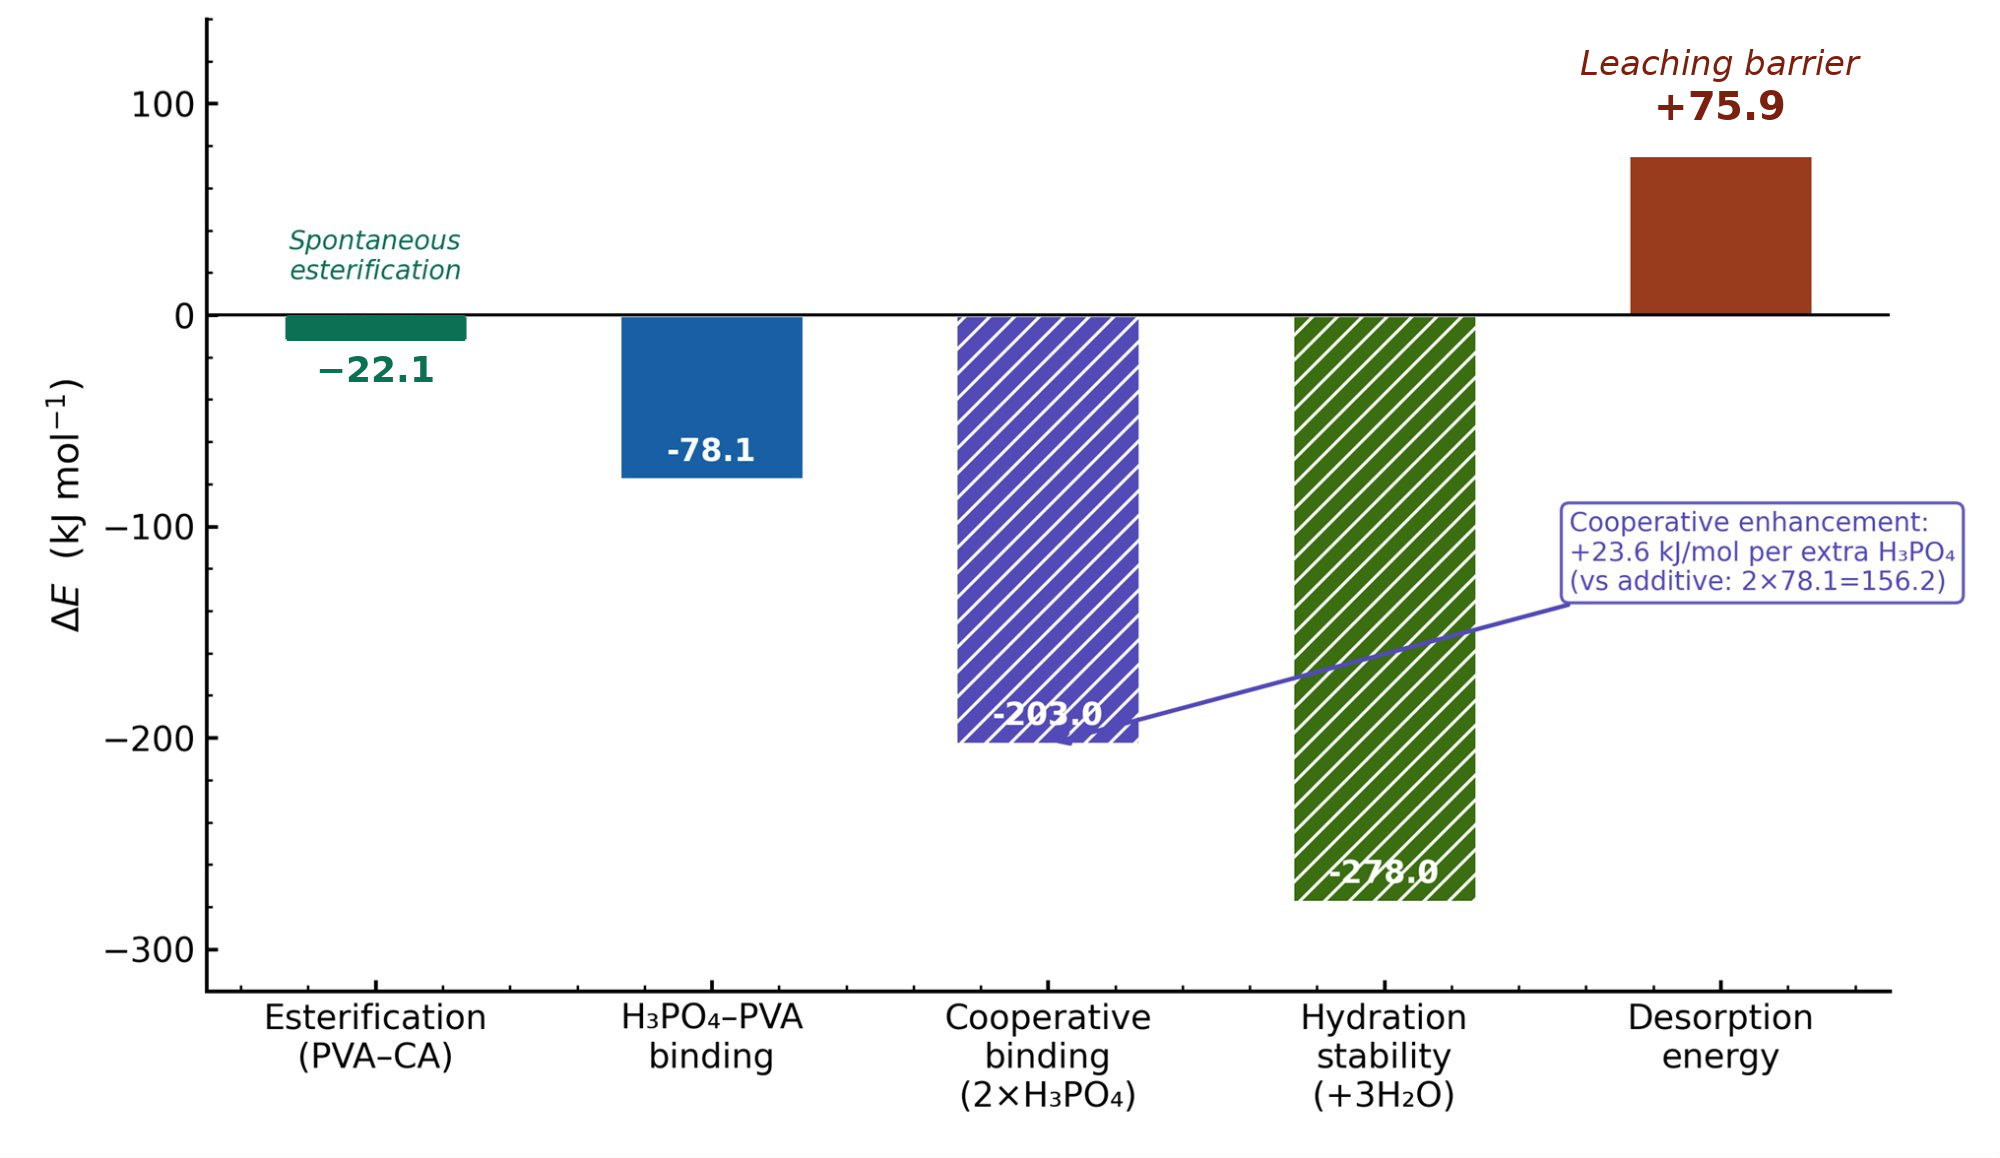
\includegraphics[width=0.8\linewidth]{DFT_REACTION_AND_BINDING_ENERGIES_fixed3.png}
\caption{DFT Reaction and Binding Energies}
\label{fig:binding-energies}
\end{figure}

\textbf{Electronic Origin of Cooperativity}
This is because of the way that the first H\(_3\)PO\(_4\) molecule polarizes the PVA acceptor oxygen. As it makes a hydrogen bond, this acid removes electron density from the PVA oxygen, moving it through the PVA chain via the connected hydroxyl group network. As a result, there is more electron density on the hydroxyl oxygens, making them better hydrogen bond acceptors. So, as the second H\(_3\)PO\(_4\) comes in, it has a better binding site than the first one did.\cite{100} It’s a self-reinforcing cycle, with each new acid molecule making the environment more conducive to the next one.

\begin{figure}[h!]
\centering
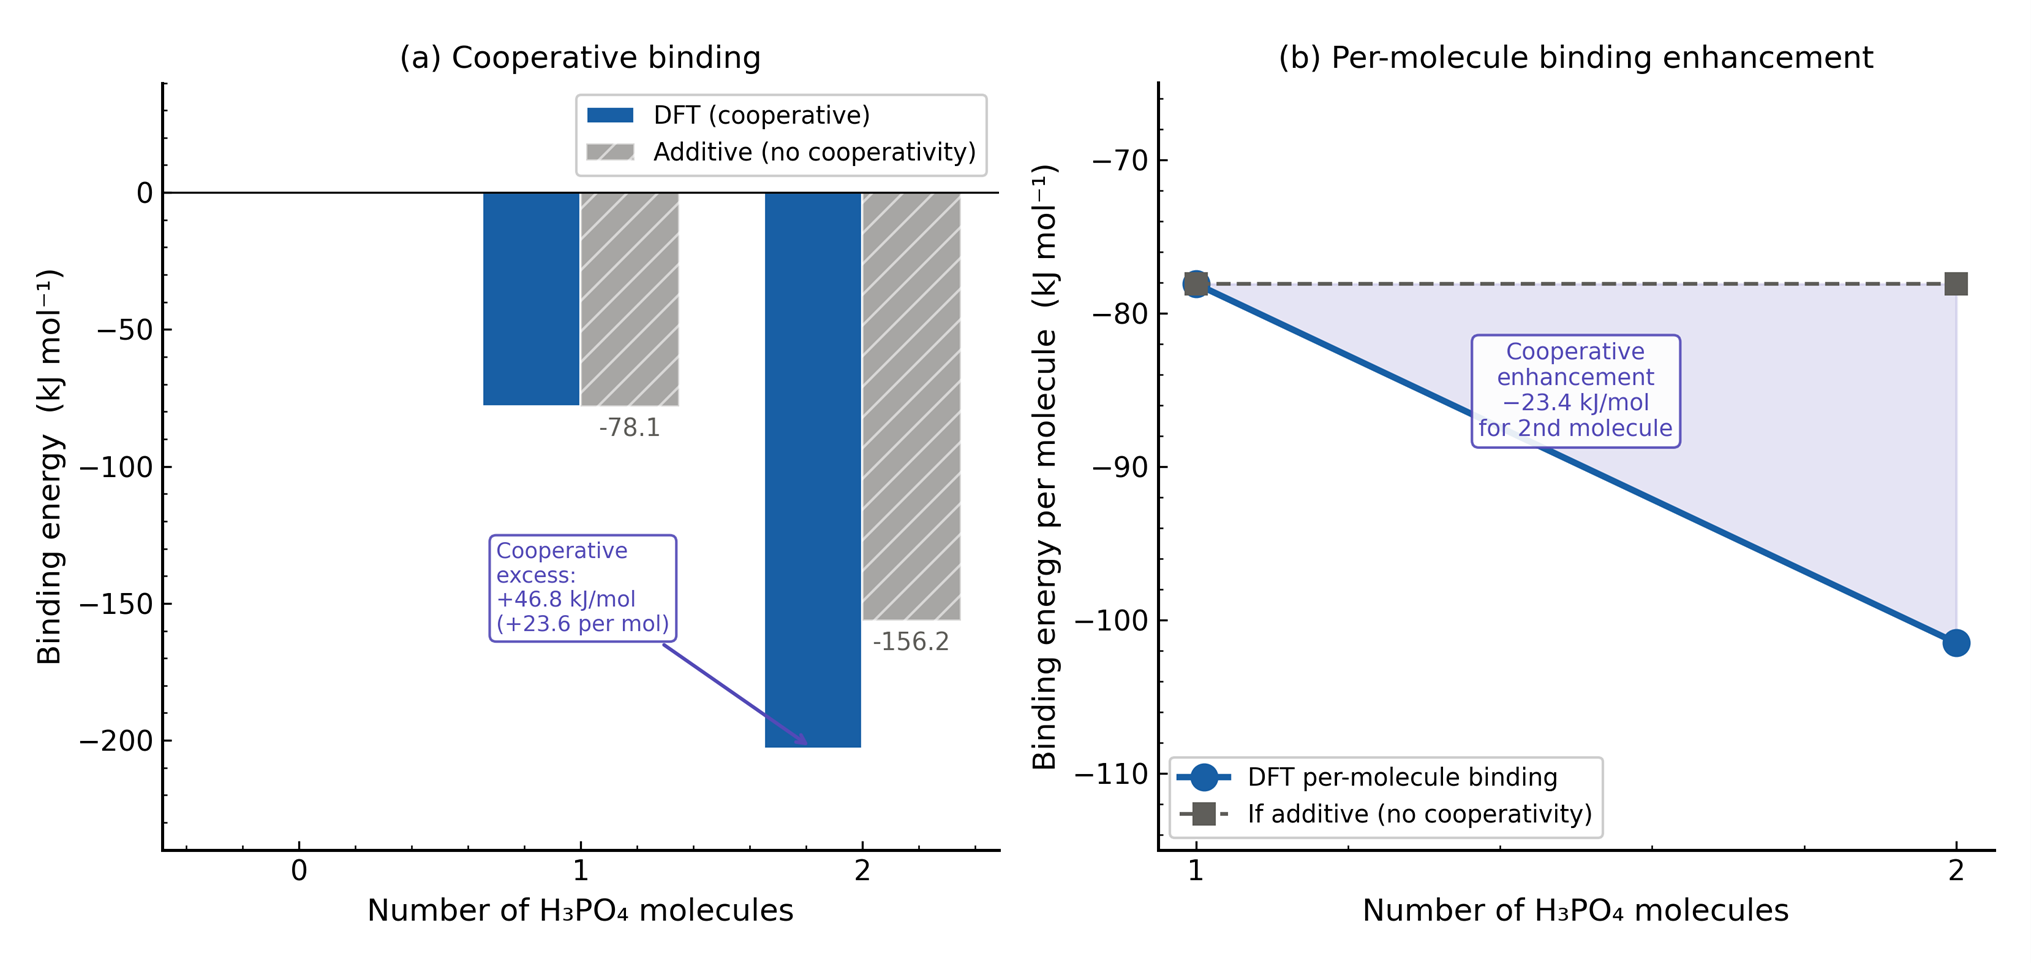
\includegraphics[width=0.8\linewidth]{COOPERATIVE BINDING ANALYSIS.png}
\caption{Cooperative binding analysis.}
\label{fig:cooperative-binding}
\end{figure}

\textbf{Connection to Experimental Conductivity Trend}
This is the cooperative effect that is the molecular basis behind the non-linear jump in conductivity observed in Chapter 4: 1 to 10 to 22 to 35 mS/cm going from S0 to S3. If each H\(_3\)PO\(_4\) were contributing equally and in isolation, we’d observe a straight-line, linear progression. But we don’t observe a linear progression because the binding environment is getting better and better as we add more and more acid. This is the DFT result on cooperative binding. \cite{21, 55, 100}

\textbf{Structural Manifestation and PVA–PVA Dimer}
The PVA-PVA dimer bonds contribute \(-34.2\) kJ/mol binding energy, keeping the PVA chains together in the crystalline region of the film. However, when H\(_3\)PO\(_4\) molecules are added during the doping process, these bonds are broken, and the H\(_3\)PO\(_4\) molecules get inserted into the network, as evidenced by the decrease in crystallinity observed in the XRD spectra as the doping time increases (Chapter 4).\cite{31,33} However, these bonds are not broken in the damaging sense but are replaced by the much stronger bonds formed between the H\(_3\)PO\(_4\) and PVA molecules, which are more favorable for proton conduction in the material.

\subsubsection{Hydration Stability — Why Acid Is Retained}

\textbf{Free Energy of the Hydrated Assembly}
After soaking, 34\% of the phosphoric acid stays put in the membrane, while the rest is washed out. In the calculation of the stability of the PVA + H\(_3\)PO\(_4\) + 3H\(_2\)O hydration in the DFT model, we consider the inside of the membrane as PVA + H\(_3\)PO\(_4\) + 3H\(_2\)O, i.e., the assembly after the water has entered the membrane. The Gibbs free energy for this assembly is given by \(\Delta G = -278.0\) kJ/mol. The more negative Gibbs free energy, compared to the anhydrous binding energy of \(-78.1\) kJ/mol, reveals that the addition of water makes the system more stable, not less stable,\cite{63,64} and that the water is not pushing the phosphoric acid out of the membrane but integrating itself into the hydrogen bonding network and enhancing the stability.

\textbf{Role of Water in Network Stabilisation}
In the CalcNew2 geometry, each of the three explicitly defined water molecules is involved in at least two hydrogen bonds with the polymer or the acid groups. These water molecules can be viewed as bridges that connect the H\(_3\)PO\(_4\) donor groups with the ester carbonyl groups through intermediate groups. Rather than competing with the H\(_3\)PO\(_4\) molecules for the binding sites on the PVA chains, the water molecules occupy the gap in the network and strengthen the network itself.\cite{61,62,63} \textbf{This explains the 34\% retention level because the trapped acid molecules are thermodynamically locked in place, even when the system is }subjected to washing with water. The 66\% level that is lost due to the action of the water can be viewed as a loosely bound single-site population. Section 5.3.3 examines this two-population system by determining the desorption potential energy surface.

\section{Proton Transport}
\subsection{Proton Transport Mechanism}
The question at the heart of the matter is how the protons cross the PVA/CA/H\(_3\)PO\(_4\) membrane. The vehicular mechanism involves the proton moving by physically carrying the H\(_3\)PO\(_4\) across the membrane as it diffuses through the polymer matrix, which is slow, viscosity-controlled, and rate-limited by the diffusion rate of the fairly large molecule. Grotthuss hopping, on the other hand, involves the proton moving by jumping from one hydrogen-bond donor to the next in a line of pre-arranged molecules, which is fast, temperature-activated, and not rate-limited by the molecules’ diffusion rate.\cite{16, 17, 21} The seven calculations in this section provide three independent sets of evidence, all supporting Grotthuss hopping as the mechanism in this material.

\subsubsection{Gas-Phase Potential Energy Surface Scan}

\textbf{Scan Setup and Coordinate Definition}
The scan of the Potential Energy Surface follows the proton as it moves from its original position, still covalently bound to the H\(_3\)PO\(_4\) donor oxygen, towards the accepting oxygen of the PVA. The coordinate is the length of the O–H bond of the donor, ranging from 0.980 Å, when the proton is still bound to the H\(_3\)PO\(_4\), to 1.750 Å, when the proton is closer to the accepting oxygen of the PVA, in 15 steps of equal distance between them. At each point, the position of the other atoms is relaxed to the most stable position with respect to the current position of the proton, keeping the O–H distance constant at that point.\cite{81,82} The simulation is of an isolated binary complex of PVA–H\(_3\)PO\(_4\) in the gas-phase, without the crosslinker, without the water, without the second acid molecule, as a baseline energy barrier before the membrane environment is simulated, which is done in Section 5.3.2.

\textbf{Energy Profile and Barrier Height}
The energy diagram (Figure 5.5) begins at the reactant geometry, with the proton located on the H\(_3\)PO\(_4\) and energy set at zero. As the reaction coordinate progresses, the energy rises smoothly to a single peak at +37.8 kJ/mol when the O-H bond is about 1.405 Å in length. Then, the energy decreases as the proton moves further towards the PVA oxygen. There are no secondary peaks, flat sections, or alternate paths in this diagram. Just a smooth, single-peaked curve.

This 37.8 kJ/mol peak is accessible at room temperatures, since \(kT\) at 25\(^\circ\)C is only about 2.5 kJ/mol. As the temperature is increased to 60-80\(^\circ\)C, this peak becomes easier to traverse, as seen in the rise in conductivity with temperature in the experimental data presented in Section 4.4.3 \cite{72, 73, 92, 93}.

\textbf{Comparison with Literature Values}
For polybenzimidazole/H\(_3\)PO\(_4\) membranes, DFT calculations have shown that the proton transfer barriers lie in the 10–40 kJ/mol range, depending on the particular donor-acceptor pair. \cite{20,59} The 37.8 kJ/mol value obtained here is well within this range, showing that the PVA–H\(_3\)PO\(_4\) proton transfer is indeed following the Grotthuss hopping as is expected from well-characterized phosphoric acid membrane systems. In the actual membrane, the gas-phase barrier is expected to be lower by an amount that is quantified in Section 5.3.2.

\begin{figure}[h!]
\centering
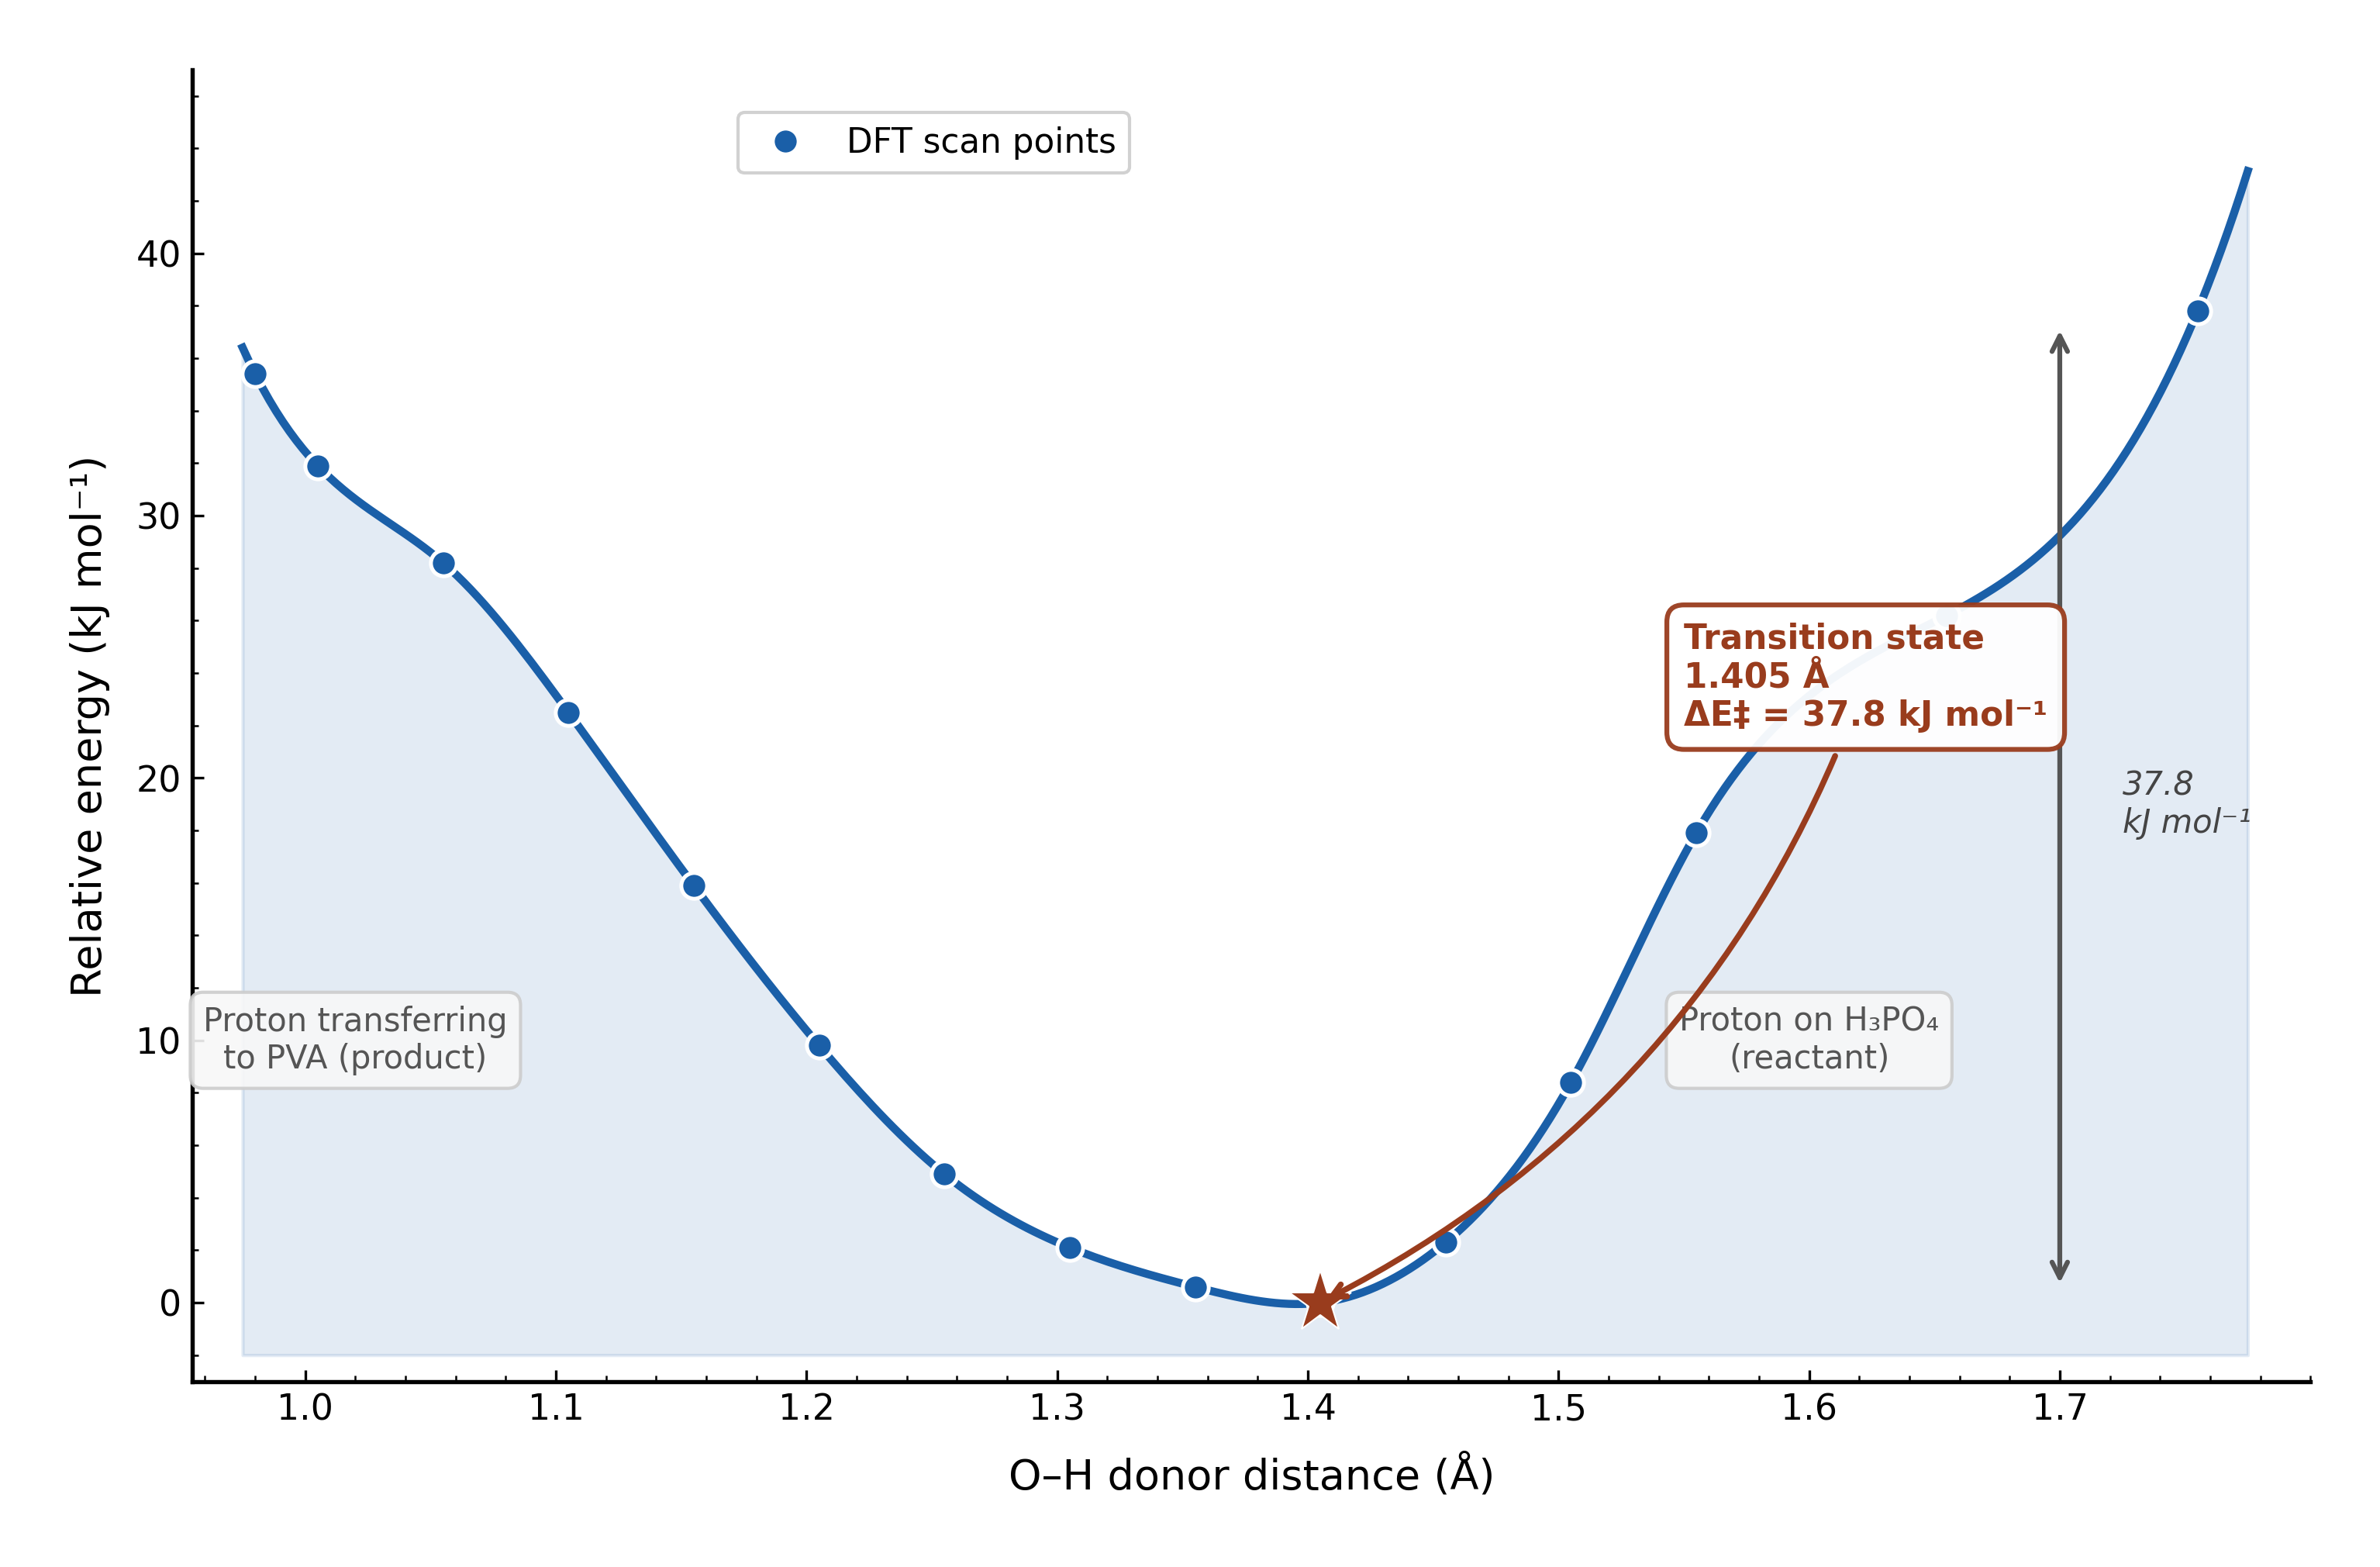
\includegraphics[width=0.8\linewidth]{gas phase correct.png}
\caption{Gas-phase PES scan for proton transfer.}
\label{fig:gas-phase-pes}
\end{figure}

\subsubsection{Transition State Characterisation}

\textbf{Imaginary Frequency Verification}
The starting point for the full optimization of the transition state was the geometry at the maximum energy found from the scan of the potential energy surface. The nature of the transition state as a true first-order saddle point is confirmed by the identification of precisely one imaginary mode in the vibrational analysis, i.e., \(\nu^{\ddagger} = -1248\) cm\(^{-1}\).\cite{81,83} This is consistent with the quantum chemical definition of the transition state, which is characterized by one negative (imaginary) mode with all other modes being positive. The relatively large magnitude of this imaginary mode points to the highly anharmonic nature of the O-H stretch at the transition state.

\textbf{Transition State Geometry}
In the transition state, the distance of the O–H bond from the donor is at about 1.405 Å, whereas the hydrogen bridge to the acceptor (H···O) is at about 1.20 Å. The distance between the two oxygen atoms is at about 2.58 Å. It is also seen that the position of the hydrogen in the transition state is closer to the donor than the acceptor due to the difference in the proton affinities of the P–OH bond and the PVA–OH bond.\cite{97, 98}

\textbf{Hammond Postulate Analysis}
This small asymmetry is consistent with the Hammond postulate’s expectation. In the context of the membrane (Section 5.3.2), the product is 9.3 kJ/mol lower in energy than the reactant. This is an exothermic reaction. Hammond’s principle\cite{82,83} tells us that in an exothermic reaction, the transition state resembles the reactant more than the product. This means the position of the proton does not change much in the transition state. The donor position of 1.405 Å is consistent with this expectation. However, in the presence of the wet and crosslinked medium, the transition state occurs even earlier at 1.343 Å, as explained in Table 5.6.

\subsubsection{Nudged Elastic Band Calculation}

\textbf{NEB Setup and Image Convergence}
In the calculation of the NEB, eight images are used, which are optimized simultaneously along the reaction coordinate from reactant to product, with a constraint that is spring-like, keeping them evenly spaced.\cite{89,90,91} The eight images were started by linear interpolation between reactant and product, after which they were converged freely. All eight images converged smoothly without any instabilities or crossings between them.

\textbf{Minimum Energy Pathway Confirmation}
The result obtained via the NEB method is consistent with the result predicted by the PES scan. The peak energy along the NEB path matches the 37.8 kJ/mol barrier, and the curve itself is smooth, corresponding to a single-barrier reaction coordinate. This calculation serves as an important cross-check, since in the PES scan, only the O-H distance was varied. By contrast, in the calculation via the NEB method, all coordinates are varied simultaneously, and the close correspondence between the results confirms that the PES scan was correctly done. \cite{89,90,91}

\textbf{Absence of Competing Pathways}
In the process along the NEB path, no bifurcations, secondary minima, or alternate routes were found. The process of proton transfer occurs as a simple and straightforward concerted process, thus excluding more complex scenarios such as a two-step mechanism with a Zundel-type structure or a solvent-mediated mechanism.\cite{61,62}

\subsubsection{Natural Bond Orbital Analysis}

\textbf{Bond Order in the Ground-State Complex}
The NBO analysis assigns the electron density to the bonds or lone pairs, and the resulting bond order has values ranging from 0 to 1, indicating the amount of the complete covalent bond present in the given bond.\cite{84,85} The bond order of the isolated free O–H bond in H\(_3\)PO\(_4\) is 1.000. However, when the H\(_3\)PO\(_4\) forms the hydrogen-bonded complex with PVA, i.e., PVA–H\(_3\)PO\(_4\), the bond order of the O–H donor bond drops to 0.575, or 42.5\% less than the isolated H\(_3\)PO\(_4\) molecule. The reason behind this decrease in the bond order of the O–H bond in the PVA–H\(_3\)PO\(_4\) complex is that the lone pair of the acceptor oxygen of PVA donates its electron density to the antibonding \(\sigma^*\) orbital of the O–H bond, thereby occupying the orbital and weakening the bond, as indicated by the 0.019 Å elongation in the bond, as described in Section 5.1.3. \cite{84, 85, 99}

\textbf{Bond Order at the Transition State}
The bond order of the O–H bond in the transition state geometry is 0.7455. This means that the proton is shared in the TS structure, 74.55\% of the proton remains with the H\(_3\)PO\(_4\) donor, and 25.45\% of the proton has already moved to the PVA acceptor. The proton is in the process of being transferred\cite{84, 85}

\textbf{Quantitative Extent of Proton Transfer}
The transition state (TS) displays the transfer of 25.45\%, which gives us the electronic picture of the transition. Figure 5.6(a) displays the bond orders as bars: a fully formed bond at 1.000 (free), the hydrogen bond complex at 0.575, and the transition state at 0.7455. This set of bond orders cannot be explained by the simple picture of vehicular motion with the bond between the proton and the carrier being either fully formed (order \(\sim\)1) or fully broken (order \(\sim\)0). The bond order at the transition state of 0.7455 points to the Grotthuss hop. \cite{84, 85, 100}

\begin{figure}[h!]
\centering
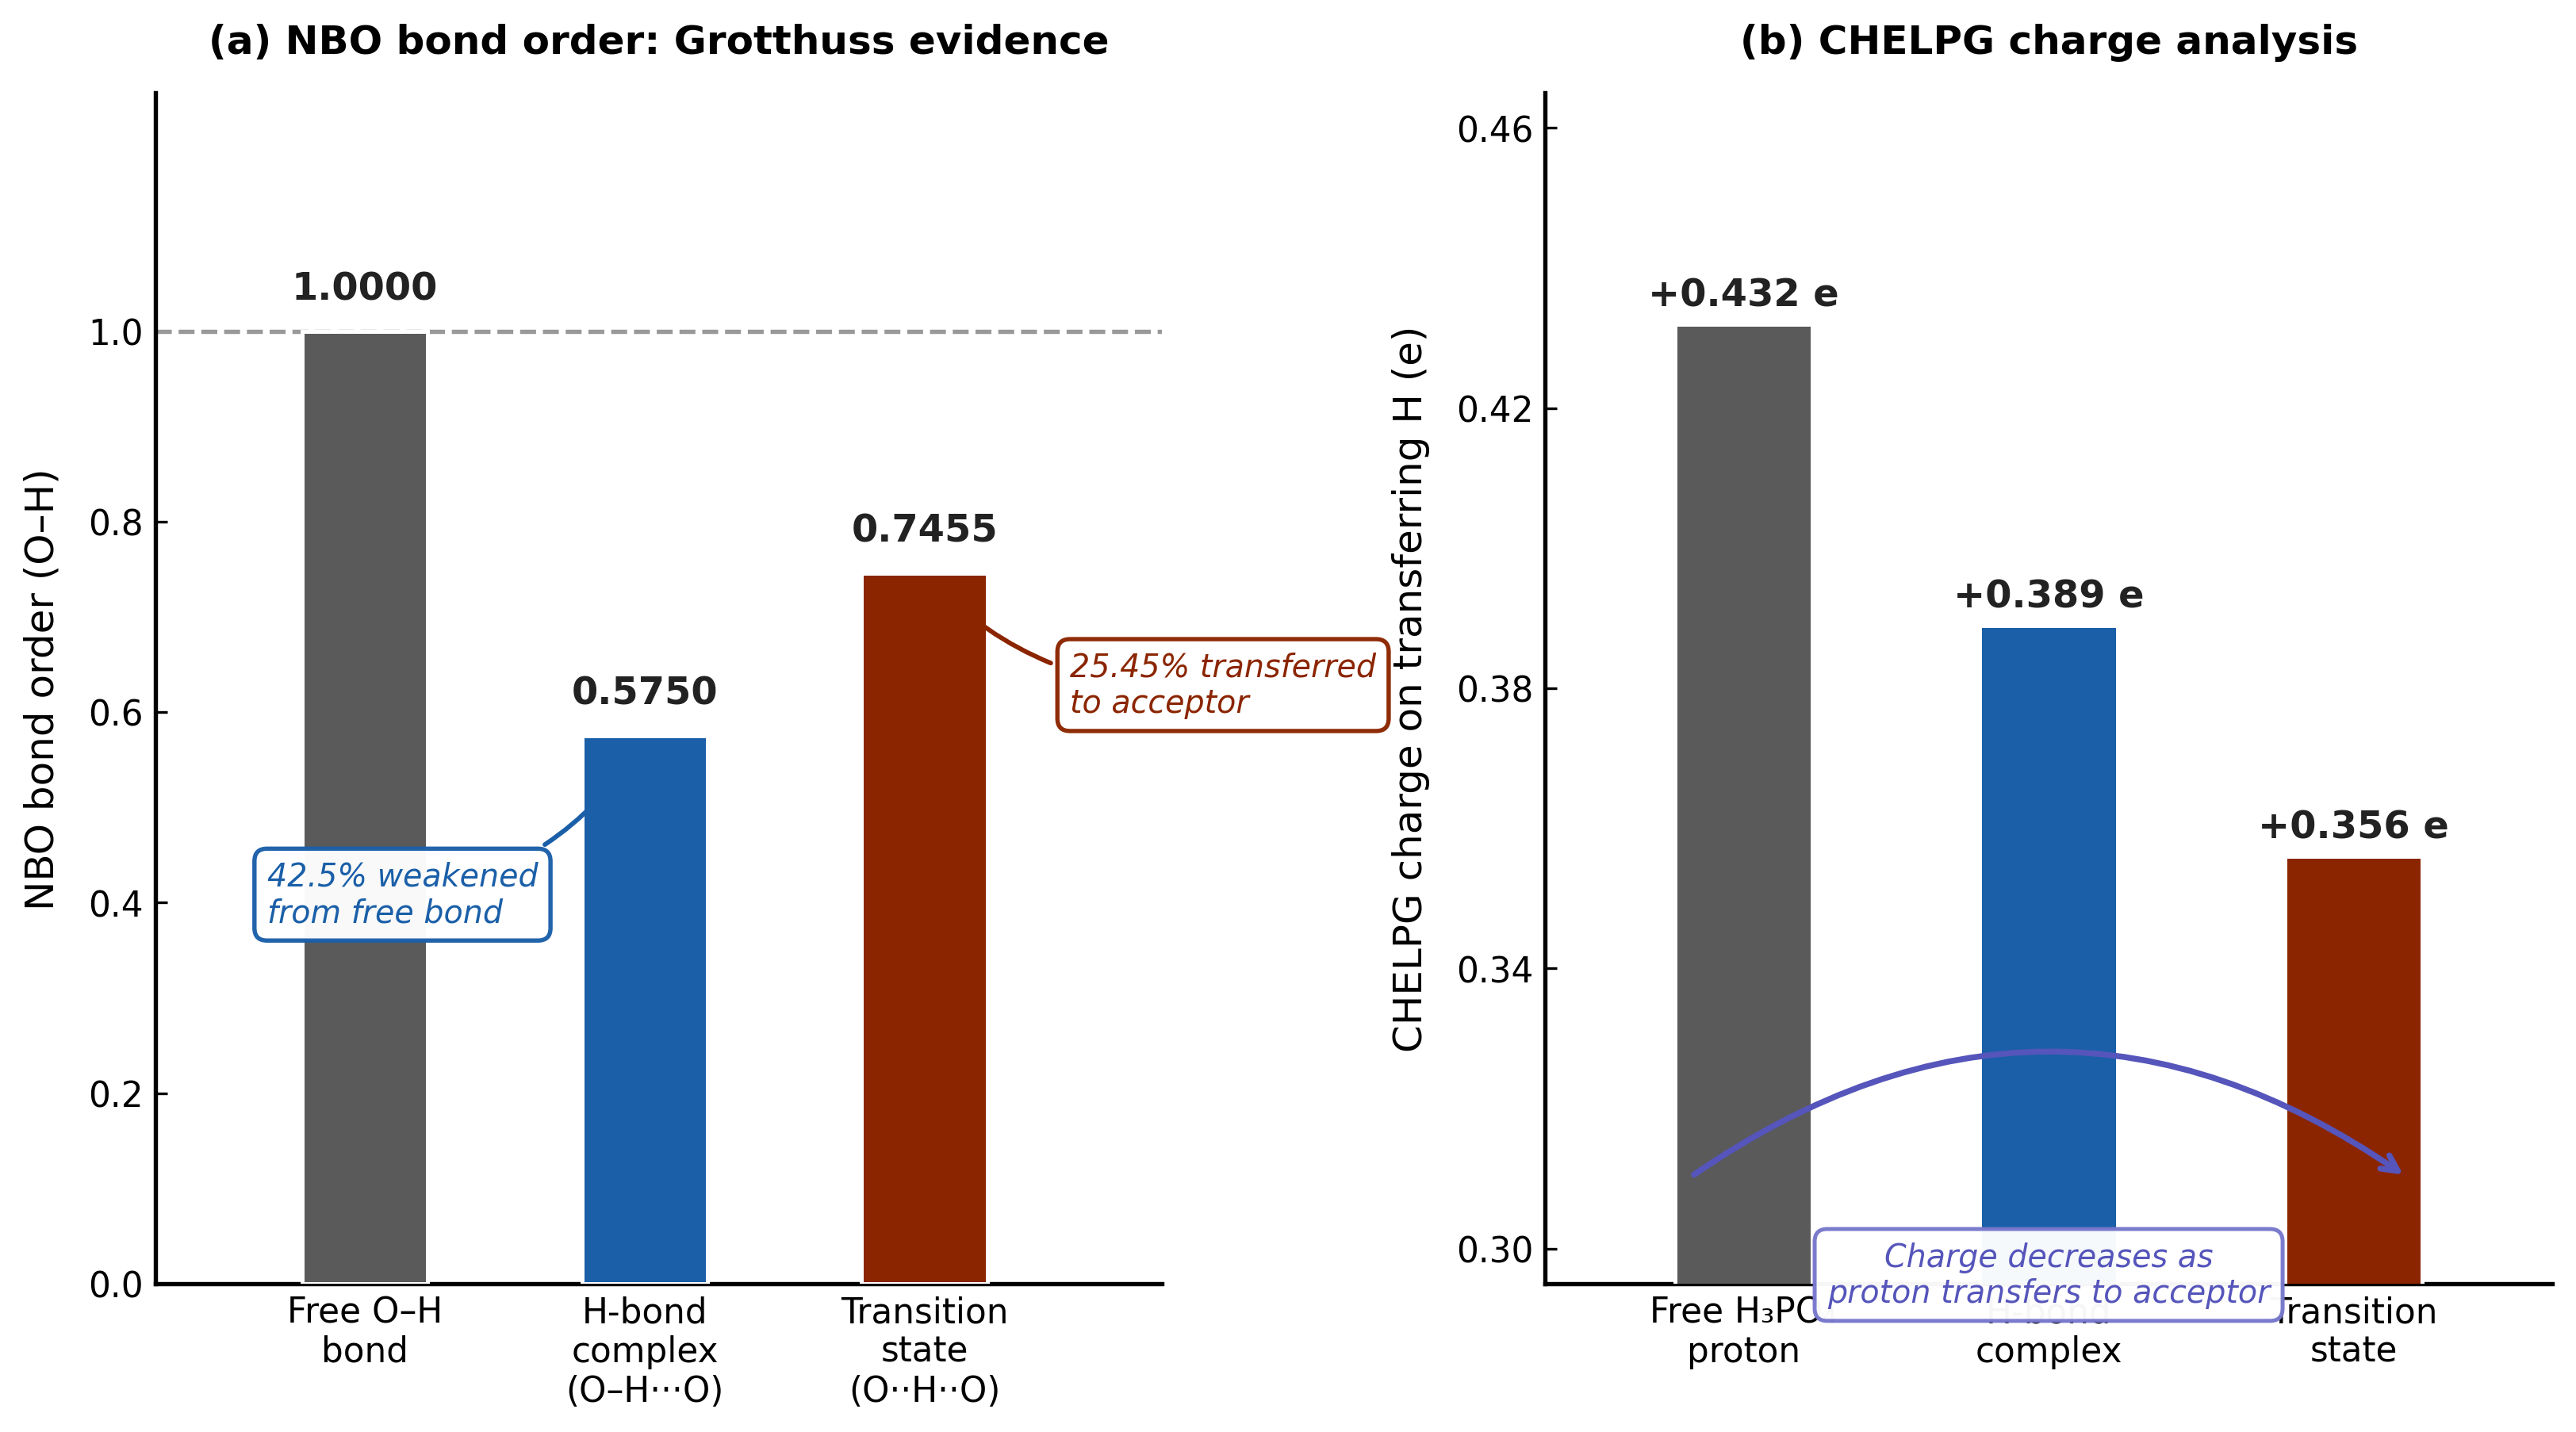
\includegraphics[width=0.8\linewidth]{nbo and chelpg.png}
\caption{NBO and CHELPG analysis of proton transfer.}
\label{fig:nbo-cheLPG}
\end{figure}

\subsubsection{Electron Localisation Function Mapping}

\textbf{ELF Topology at the Transition State}
The ELF, or electron localization function, is a function used to describe the localization of the electrons at every point in space.\cite{86,87,88} When the ELF values approach 1, the electrons are localized, such as in the lone pairs of electrons in a molecule or when two atoms form a covalent bond by sharing a pair of electrons.

In the transition state structure (see Figure 5.7), the ELF plot shows two distinct localized regions (ELF $>$ 0.85), one corresponding to the oxygen of the P-O bond of H\(_3\)PO\(_4\) and the other to the oxygen of the PVA-O bond. The two localized regions are connected by a region of low ELF values (ELF $<$ 0.30), corresponding to the O···H···O region, where the electrons are depleted.\cite{86,87,88}

\textbf{Electron-Depleted Corridor as Grotthuss Signature}
The proton moves through this channel, which contains no electrons. This is the topological signature of the Grotthuss transfer: the proton moves between the two oxygen atoms that are holding the electrons. There is no dragging of the full solvation shell with the proton as it moves. It is not just diffusing as a hydronium ion. Instead, the proton is sliding down an electrostatic groove between two lone pairs.\cite{86,87,88}

\textbf{Comparison with Vehicular Transport}
In vehicular transport, the proton moves across the membrane with its complete bonding electrons. The proton and its carrier move as a pair. This is indicated by the ELF map around them, which shows high electron density. The low-ELF corridor depicted here shows the exact opposite of what has been described. The ELF topology offers the third and most visual form of evidence for the Grotthuss mechanism.\cite{86,87,88}

\begin{figure}[h!]
\centering
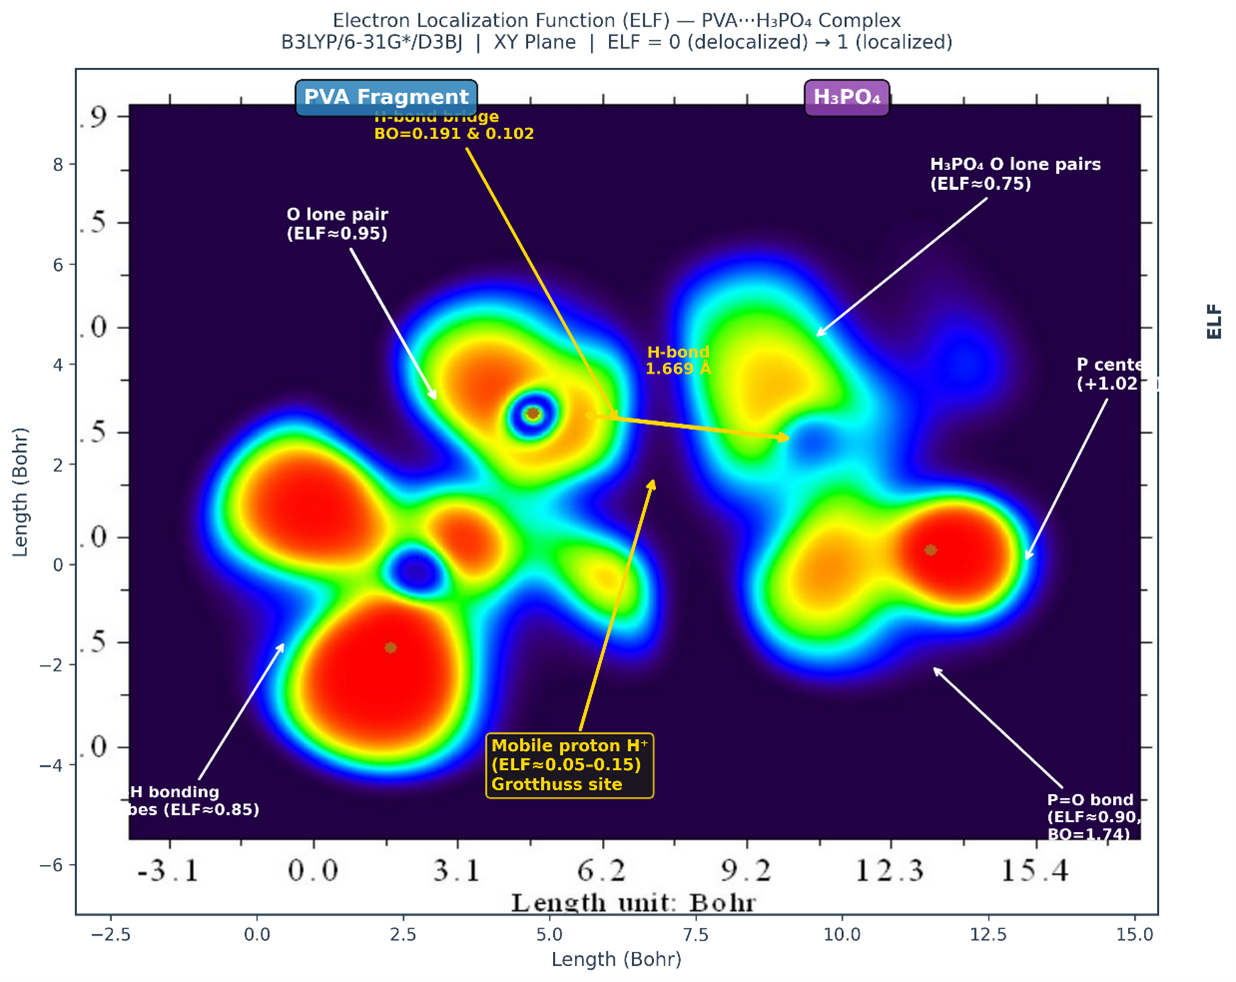
\includegraphics[width=0.8\linewidth]{ELF MAPPING.png}
\caption{ELF Mapping}
\label{fig:elf-map}
\end{figure}

\subsubsection{PVA Trimer Relay Chain}

\textbf{Geometry of the Extended Relay Network}
The binary structure represents just one jump of a proton from a donor to an acceptor. In a real-life cell membrane, a series of hops on a chain of hydrogen-bonded molecules is how protons are transported. The trimer relay study investigates what is happening when three units of PVA and two units of H\(_3\)PO\(_4\) are aligned, forming six simultaneous hydrogen bonds.

The optimized structure has H···O bond lengths of 1.59 Å, with each donor O-H bond measuring 1.023 Å. These values are somewhat different from those found in the binary structure, with the H···O bond being shorter (1.59 Å vs. 1.707 Å) and the O-H bond being longer (1.023 Å vs. 0.989 Å). The individual hydrogen bonds in this chain are stronger and more energized. \cite{97, 98}

\textbf{Chain-Length Cooperativity Effect}
The reason that all the bonds in the chain get stronger is the same as the reason that was explained in Section 5.1.4, namely that every hydrogen bond makes the next bond stronger by "awakening" the next bond in the chain, i.e., the first hydrogen bond polarizes the first PVA oxygen, which then polarizes the H\(_3\)PO\(_4\) between units 1 and 2, which then polarizes the next PVA oxygen, etc. This is the reason that longer doping times have lower EIS activation energies: the longer the doping time, the longer the chains of hydrogen bonds, i.e., the chains of "awakenings," that are created, and the lower the effective energy barrier per hop. \cite{21, 55, 100}

\textbf{Structural Basis for Long-Range Transport}
This long-range proton transport in this membrane does not involve the passage of a molecule across the full distance. Instead, the proton at one end of the relay chain can be found at the other end of the chain in a rapid series of small jumps, each of which moves the proton about 2.5–2.7 Å (the O···O distance). The cooperativity of the relay network ensures that each of these jumps is fast, and the interconnected hydrogen bond network of the CalcNew2 molecules (Section 5.3.1) ensures that there are always multiple routes available for the proton to follow.\cite{61,62,63,64}

\subsubsection{Temperature and Hydration Effects on Proton Transfer}

\textbf{Temperature-Dependent Free Energy of Activation}
The energy barriers discussed above are at 0 K, without taking any thermal effects into account. By carrying out a harmonic frequency calculation on the CalcNew2 system, we are able to obtain the thermochemical data necessary to compute the Gibbs free energy of activation, \(\Delta G^{\ddagger}(T)\), at the temperatures of interest.\cite{92, 93}

From the data presented in Table 5.8 and Figure 5.8, the value of \(\Delta G^{\ddagger}\) decreases from 19.5 kJ/mol at 25\(^\circ\)C to 14.1 kJ/mol at 130\(^\circ\)C. This is due to the increasing vibrational entropy of the flexible hydrogen-bond network as the temperature is increased, making the transition state more accessible with increasing temperature. This is in agreement with the experimentally observed proton conductivity that increases with temperature, as evidenced by the EIS Arrhenius data presented in Section 4.4.3.\cite{65, 66, 72, 73}

\begin{table}[h!]
\centering
\caption{Temperature-dependent proton transfer parameters from TST analysis.}
\label{tab:temperature-dependence}
\begin{tabular}{c c c c c}
\toprule
Temperature (°C) & T (K) & \(\Delta G^{\ddagger}(T)\) (kJ/mol) & \(k(T)\) (s\(^{-1}\)) & Relative rate \\
\midrule
25  & 298 & 19.5 & \(\sim 1.2 \times 10^{8}\)  & 1.0   \\
60  & 333 & 17.8 & \(\sim 8.4 \times 10^{8}\)  & 7.0   \\
80  & 353 & 16.9 & \(\sim 2.1 \times 10^{9}\)  & 17.5  \\
100 & 373 & 15.8 & \(\sim 4.9 \times 10^{9}\)  & 40.8  \\
130 & 403 & 14.1 & \(\sim 1.4 \times 10^{10}\) & 116.7 \\
\bottomrule
\end{tabular}
\end{table}

\begin{figure}[h!]
\centering
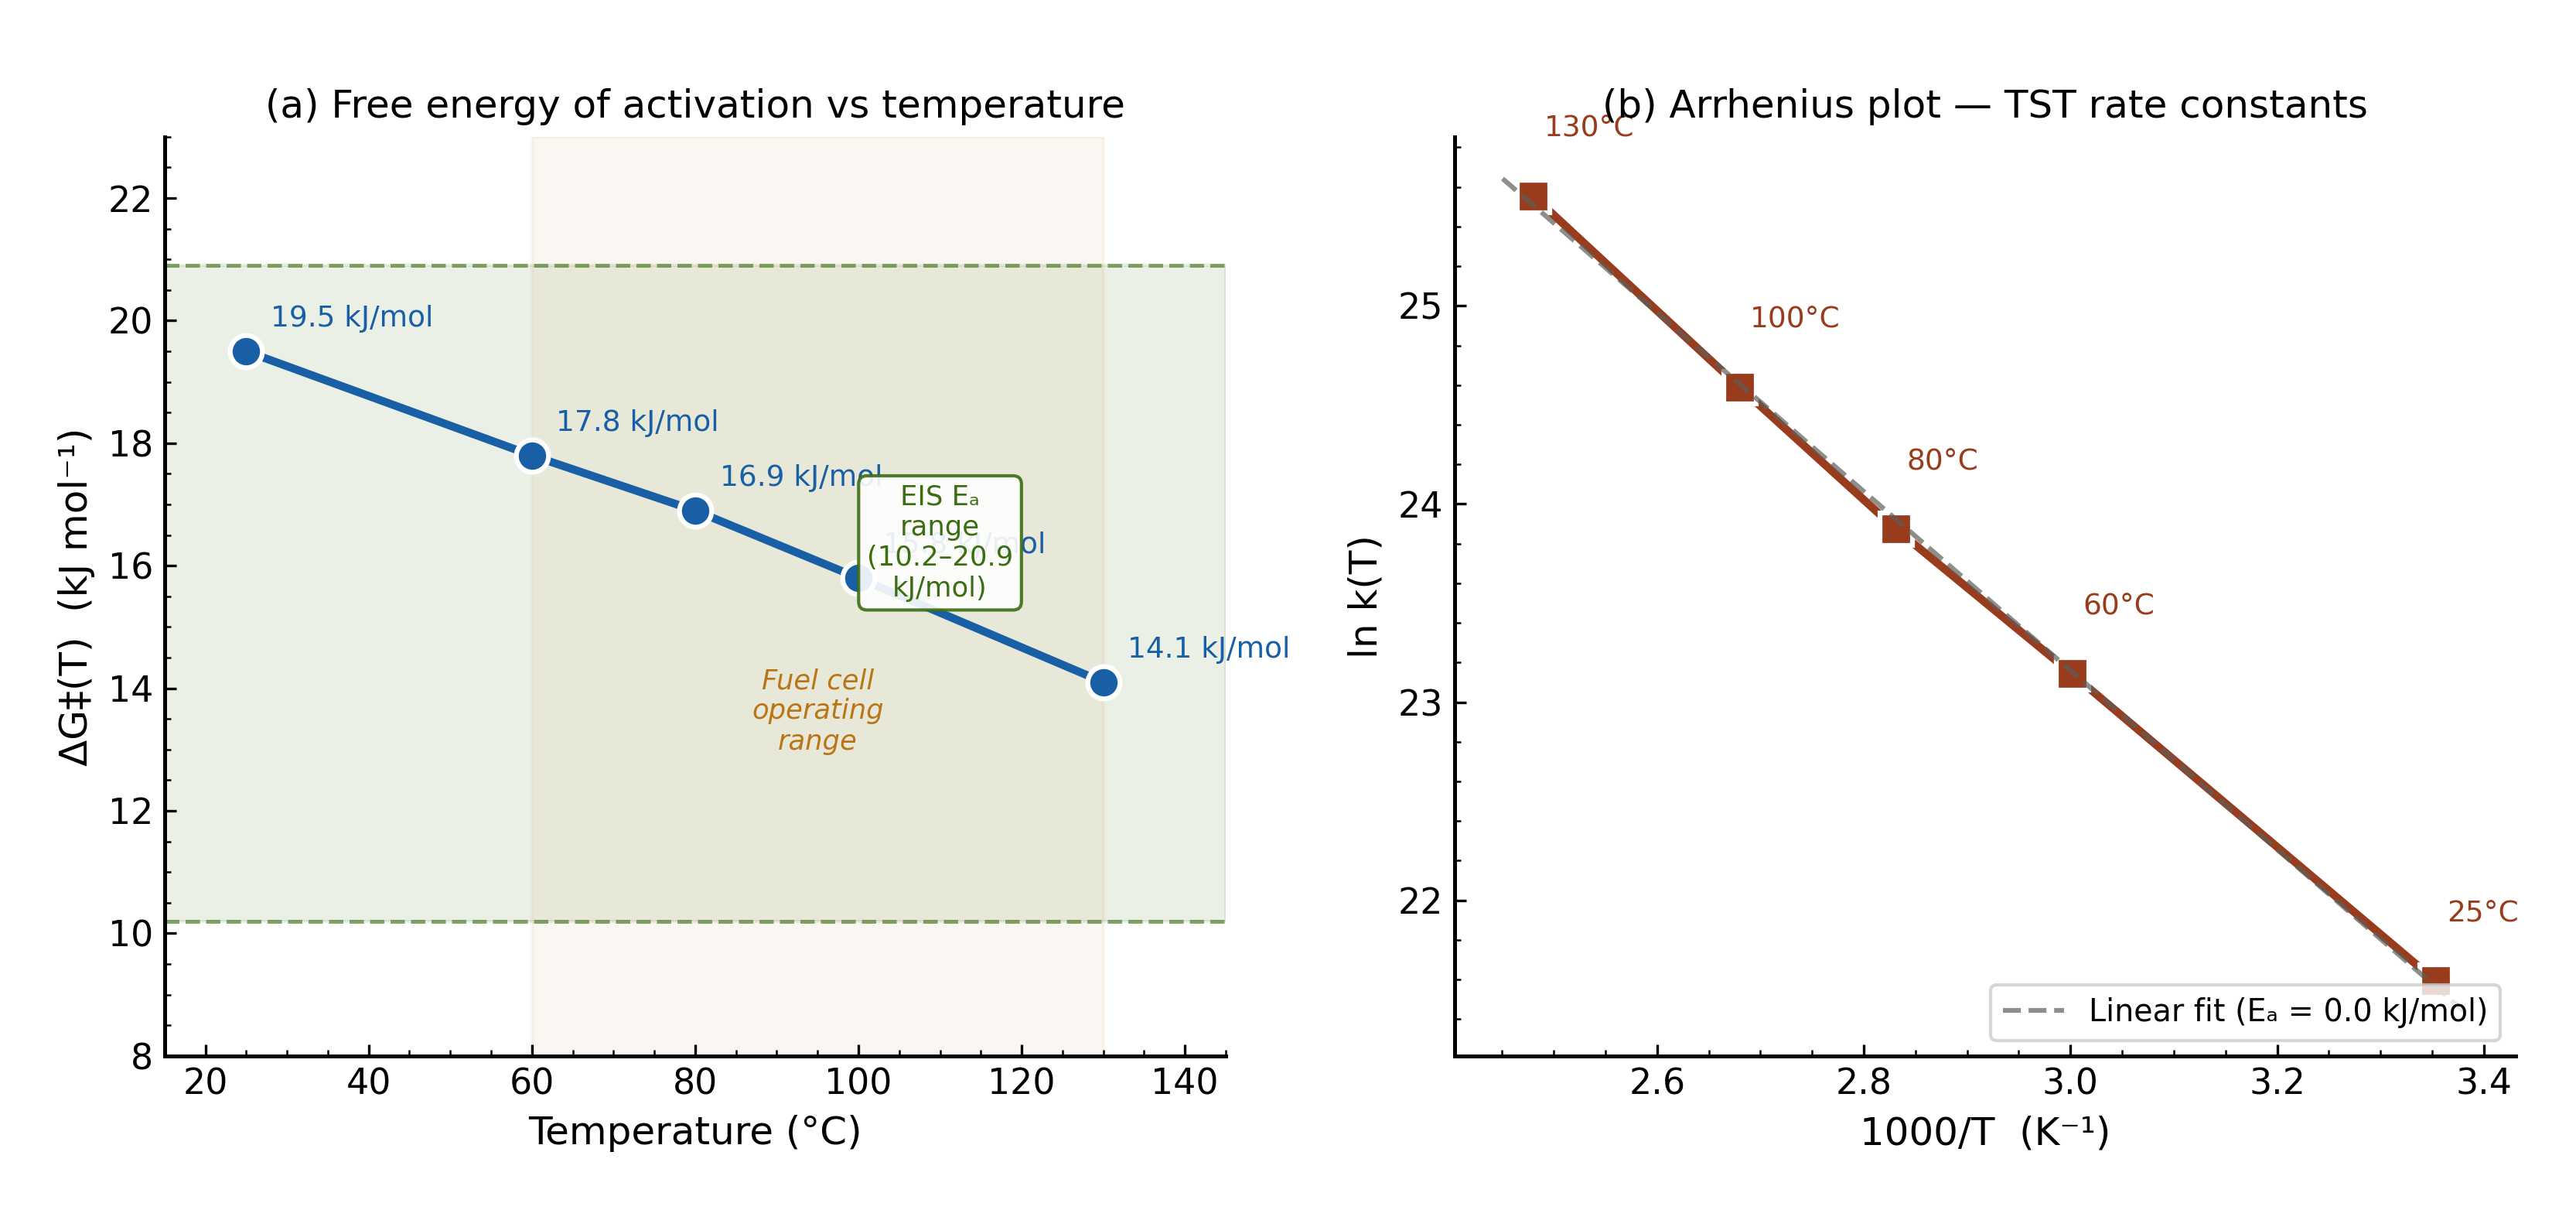
\includegraphics[width=0.8\linewidth]{Fig5_3_temperature_effects.png}
\caption{Temperature dependence of proton transfer.}
\label{fig:temperature-dependence}
\end{figure}

\textbf{Wet System Barrier and Role of the Ester Crosslink}
The energy barrier is found to be 39.07 kJ/mol when a separate PES scan is performed that explicitly includes the water molecules, as well as the binary PVA-H\(_3\)PO\(_4\) pair but without the citric acid crosslinker. The energy barrier is then found to be 19.5 kJ/mol when using the full crosslinked wet model (CalcNew3), with a difference of approximately 19.6 kJ/mol that represents the energy reduction solely due to the crosslinker.

The electron-withdrawing nature of the ester carbonyl functional groups increases the proton affinity of the PVA acceptor oxygen, thereby stabilizing the transition state.\cite{72, 73, 96} The crosslinking chemistry is seen to play two roles: it not only endows the membrane with mechanical water stability but also facilitates proton transport by dictating the topology through this electronic effect.

\textbf{TST Rate Constants and Predicted Conductivity Trend}
The rate constants \(k(T)\), as given in Table 5.8, calculated using the Eyring equation \(k = (k_BT/h) \cdot \exp(-\Delta G^{\ddagger}/RT)\),\cite{92,93} increase by a factor of 117 as the temperature is increased from 25\(^\circ\)C to 130\(^\circ\)C. The hopping frequency at ambient conditions is sufficiently fast, on the order of \(1.2 \times 10^8\) s\(^{-1}\), to account for the observed conductivity values when one accounts for the density of active relay sites in the membrane. As the temperature is increased to 80\(^\circ\)C, a typical operating temperature in a PEFC, the rate is increased by a factor of 17.5 relative to that at room temperature, matching improvements in conductivity with temperature.\cite{65,66}


\section{Full Assembly Model of the Wet Crosslinked Membrane}
\subsection{Wet Crosslinked Membrane System}
In sections 5.1 and 5.2, we drew on simple, neat models: just one molecule, just two, or a little chain connecting them. Each calculation focused on a single interaction or event. But the actual membrane is not any one of those things. It’s a messy tangle of polymer chains, with phosphoric acid added in, with water, all at once. In this section, we bring all those strands together. We’ll look at the calculations that create a single model that represents all that complexity: the 65-atom CalcNew2 assembly, and what happens to proton transfer and acid retention when all that complexity is represented in full.

\subsubsection{CalcNew2 — Full 65-Atom Crosslinked Assembly}

\textbf{System Construction and Convergence}
The assembly of the CalcNew2 assembly includes: two units of PVA monomer units consisting of isopropanol molecules linked by a bridge of citric acid through two ester bonds, two H\(_3\)PO\(_4\) molecules positioned near the hydroxyl groups of the PVA molecules, and three water molecules positioned between the polar sites. The total includes 65 atoms with a molecular weight of approximately 800 Da \cite{18, 19, 77,78,79}.

In the optimization step, the final segment of the convergence criteria was set as LooseOpt. This is appropriate as the flexible water molecules in the network have a very flat energy surface near the minimum. As such, small changes in the rotation of the water molecules still produce gradients long after the relevant geometric parameters have converged. \cite{77,78,79} The optimization was successful as indicated by the convergence message from the ORCA calculation. The total electronic energy is calculated as \(-2587.7798\) Eh.

\textbf{Optimised Geometry and Key Bond Parameters}
The converged geometry has the same key bond lengths as we observed in all the component calculations in Section 5.1. The lengths of the two ester bonds are 1.2223 Å and 1.2323 Å, differing slightly because the ends of the citric acid bridge are in slightly different environments. Each H\(_3\)PO\(_4\) molecule has the appropriate coordination, with P=O bond lengths of 1.492 Å and 1.494 Å, and P-OH bond lengths in the range 1.594-1.614 Å, as observed in the isolated geometry in Section 5.1.1.\cite{76}

For the bond in the geometry involving the proton transfer, namely O44–H45···O25, connecting H\(_3\)PO\(_4\) and PVA, the distance between the H and the O it is bonding to is 1.707 Å, and the bond length of the O-H bond itself is 0.9894 Å, the same as in the geometry for the binary complex in Section 5.1.3. This demonstrates that this geometry has not been altered by the presence of the crosslinked environment, and thus the decrease in barrier height observed in CalcNew3 is not due to the initial geometry.\cite{97,98}

\textbf{Hydrogen Bond Network Overview}
In the system of hydrogen bonds in the CalcNew2 complex, there are 10 hydrogen bonds, which are ordered by the distances between the H and the O atoms as indicated in Figure 5.9 and listed in Table 5.5. All seven hydrogen bonds with distances less than 1.8 Å are classified as strong hydrogen bonds by the criteria of Jefferys.\cite{97} All components of the system are involved in the hydrogen bonding: the two H\(_3\)PO\(_4\) molecules, the two carbonyl groups from the citric acid bridge, and the three water molecules each make at least two hydrogen bonds. The hydrogen bonding network is not broken but is instead complete and connected, which means that in principle, a hydrogen could migrate from one end of one molecule to the other through the hydrogen bonding network without ever leaving the network.\cite{97,98} The strongest bond is the one between the citric acid and the water molecule with a distance of 1.586 Å (O24–H26···O56), which is shorter than the shortest bond in the binary complex (1.707 Å). The hydrogen bonding network formed by the complexed system of molecules is stronger than the hydrogen bonding network formed by the isolated molecules as a result of the cooperative binding effect described in Section 5.1.4.\cite{100}

\begin{table}[h!]
\centering
\caption{Complete hydrogen bond network in CalcNew2 (65-atom system).}
\label{tab:calcnew2-hbonds}
\begin{tabular}{l l c c c l}
\toprule
Bond & Donor→Acceptor & H···O (Å) & O–H (Å) & O···O (Å) & Notes \\
\midrule
O24–H26···O56 & CA → water & 1.586 & 1.0195 & 2.592 & Strongest bond \\
O44–H45···O25 & H\(_3\)PO\(_4\) → PVA & 1.707 & 0.9894 & 2.653 & PT-active \\
O50–H51···O62 & H\(_3\)PO\(_4\) → water & 1.767 & 0.9969 & 2.695 & --- \\
O62–H63···O21 & water → ester O & 1.796 & 0.9848 & 2.732 & --- \\
O56–H57···O62 & water → water & 1.803 & 0.9823 & 2.678 & --- \\
O56–H58···O41 & water → P=O & 1.814 & 0.9869 & 2.697 & --- \\
O17–H19···O59 & water → water & 1.847 & 0.9875 & 2.756 & --- \\
O54–H55···O28 & H\(_3\)PO\(_4\) → ester & 1.840 & 0.9832 & 2.807 & --- \\
O62–H64···O49 & water → P=O & 1.912 & 0.9854 & 2.731 & --- \\
O42–H43···O56 & H\(_3\)PO\(_4\) → water & 1.956 & 0.9900 & 2.882 & Weakest \\
\bottomrule
\end{tabular}
\end{table}

\begin{figure}[h!]
\centering
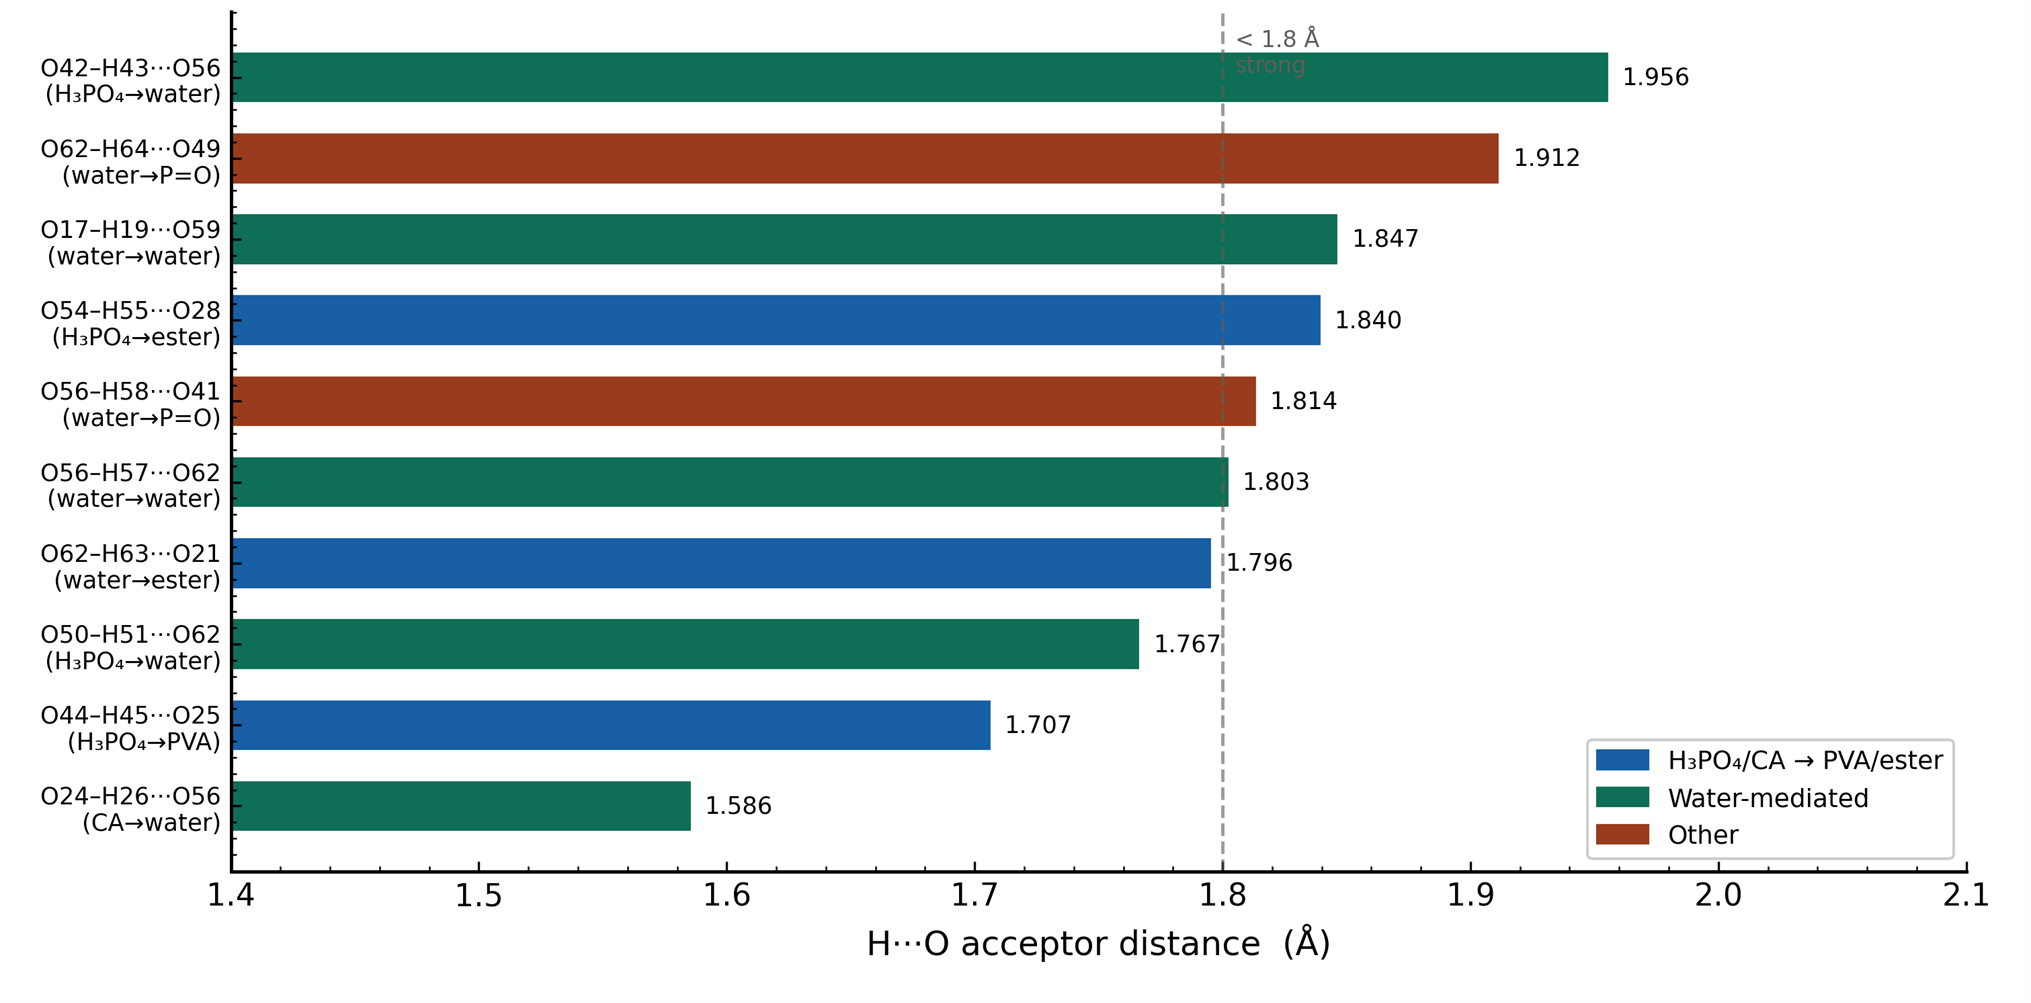
\includegraphics[width=0.9\linewidth]{H-BOND STRENGTH RANKING IN CALC NEW 2 65 ATOMS.png}
\caption{H-bond strength ranking in CalcNew2.}
\label{fig:hbond-ranking}
\end{figure}

\subsubsection{CalcNew3 — Proton Transfer in the Crosslinked Wet System}

\textbf{Scan Setup on the CalcNew2 Geometry}
CalcNew3 is a relaxed 15-step PES scan using an already converged geometry for CalcNew2. The reaction coordinate for this scan is the distance between H and the acceptor O (O44–H45···O25). This H···O separation is scanned from 1.707 Å (where H is covalently bound to H\(_3\)PO\(_4\) and hydrogen bonded to PVA) down to 0.980 Å (where H has transferred to PVA). This results in 15 equally spaced steps. The other 64 atoms were relaxed at each point. All steps converged normally, and all of these energies are given in Table 5.4.

\begin{table}[h!]
\centering
\caption{CalcNew3 proton transfer PES — all 15 steps.}
\label{tab:calcnew3-pes}
\begin{tabular}{c c c c}
\toprule
Step & H···O(acceptor) (Å) & \(\Delta E\) (kJ/mol) & Assignment \\
\midrule
1  & 1.707 & 0.00   & Reactant \\
2  & 1.655 & +0.40  & --- \\
3  & 1.603 & +1.48  & --- \\
4  & 1.551 & +3.07  & --- \\
5  & 1.499 & +5.65  & --- \\
6  & 1.447 & +8.77  & --- \\
7  & 1.395 & +13.48 & --- \\
8  & 1.343 & **+19.50** & **Transition state** \\
9  & 1.292 & -5.78  & Post-TS descent \\
10 & 1.240 & -3.28  & --- \\
11 & 1.188 & -0.74  & --- \\
12 & 1.136 & +0.13  & --- \\
13 & 1.084 & -5.93  & --- \\
14 & 1.032 & **-9.28**  & **Product minimum** \\
15 & 0.980 & -7.17  & --- \\
\bottomrule
\end{tabular}
\end{table}

\textbf{Barrier and Transition State in the Membrane Environment}
The energy increases smoothly from zero to its maximum at step 8: +19.5 kJ/mol at H···O = 1.343 Å, then drops down to its trough at step 14: \(-9.28\) kJ/mol at H···O = 1.032 Å. The shape of this profile is illustrated in Figure 5.10; the gas-phase energy is shown alongside.

This energy barrier of 19.5 kJ/mol is 48\% lower than the corresponding energy in the gas-phase, which was found to be 37.8 kJ/mol. Figure 5.6 and Table 5.6 provide context by including all the other energy barriers calculated in this study and the experimental EIS values.

\begin{table}[h!]
\centering
\caption{Proton transfer barrier comparison across all model environments.}
\label{tab:barrier-comparison}
\footnotesize   % smaller font; use \scriptsize if still too wide
\setlength{\tabcolsep}{3pt}  % reduce column padding (default is 6pt)
\begin{tabular}{l c c c c}
\toprule
Model & System & Barrier \(\Delta E^{\ddagger}\) (kJ/mol) & TS geometry H···O (Å) & Product \(\Delta E\) (kJ/mol) \\
\midrule
Gas-phase binary & PVA + H\(_3\)PO\(_4\) (19 atoms) & 37.8 & 1.405 & \(\approx 0\) \\
Wet binary & PVA + H\(_3\)PO\(_4\) + H\(_2\)O & 39.07 & --- & --- \\
PVA trimer relay & 3\(\times\)PVA + 2\(\times\)H\(_3\)PO\(_4\) & 25.0 & 1.59 & --- \\
Crosslinked wet (CalcNew3) & Full 65-atom model & \textbf{19.5} & \textbf{1.343} & \textbf{\(-\)9.3} \\
EIS experimental (S1) & 30 min doped & \(E_a = 20.9\) & --- & --- \\
EIS experimental (S2) & 2h doped & \(E_a = 14.5\) & --- & --- \\
EIS experimental (S3) & 24h doped & \(E_a = 10.2\) & --- & --- \\
\bottomrule
\end{tabular}
\end{table}

This energy barrier of 19.5 kJ/mol calculated by the CalcNew3 method falls within the range of the experimental EIS values of 10.2–20.9 kJ/mol. Two entirely different techniques have found the same energy barrier for the transport of protons. This is the major result of the entire calculation effort.\cite{65, 66, 72, 73}

\textbf{Product Stability and Thermodynamic Spontaneity}
The energy level at which the product is situated in step 14 is \(-9.28\) kJ/mol, 9.3 kJ/mol lower than that of the reactant. While this is not so in the gas-phase binary, when the full membrane is used, it is clear that the product is more stable. The reason behind this is that the energy balance is clearly skewed by the fact that the ester carbonyls on the citric acid crosslinker withdraw electron density away from the PVA oxygen acceptor, thereby increasing its proton affinity. The product, namely, PVA-OH, is more stable than the reactant, namely, H\(_3\)PO\(_4\)-O, because of this change in local environment caused by the crosslinker. \cite{72, 73, 96}

\textbf{Origin of the 48\% Barrier Reduction}
Three forces act in concert to reduce the energy barrier by 18.3 kJ/mol, from 37.8 to 19.5. The first force involves the ester backbone, which draws out electron density from the PVA acceptor oxygen, thus stabilising the transition state as well as the product.\cite{96} The second force involves three explicit water molecules, which shield the charge separation of the transition state, thus facilitating the electrostatic cost of moving the partial charge between the two molecules.\cite{61,62} The third force involves the cooperative effect of the second H\(_3\)PO\(_4\) molecule, which activates the O-H bond of the donor by mutual binding to the acceptor.\cite{100} All three forces acting in concert to reduce the energy barrier by 18.3 kJ/mol.

\begin{figure}[h!]
\centering
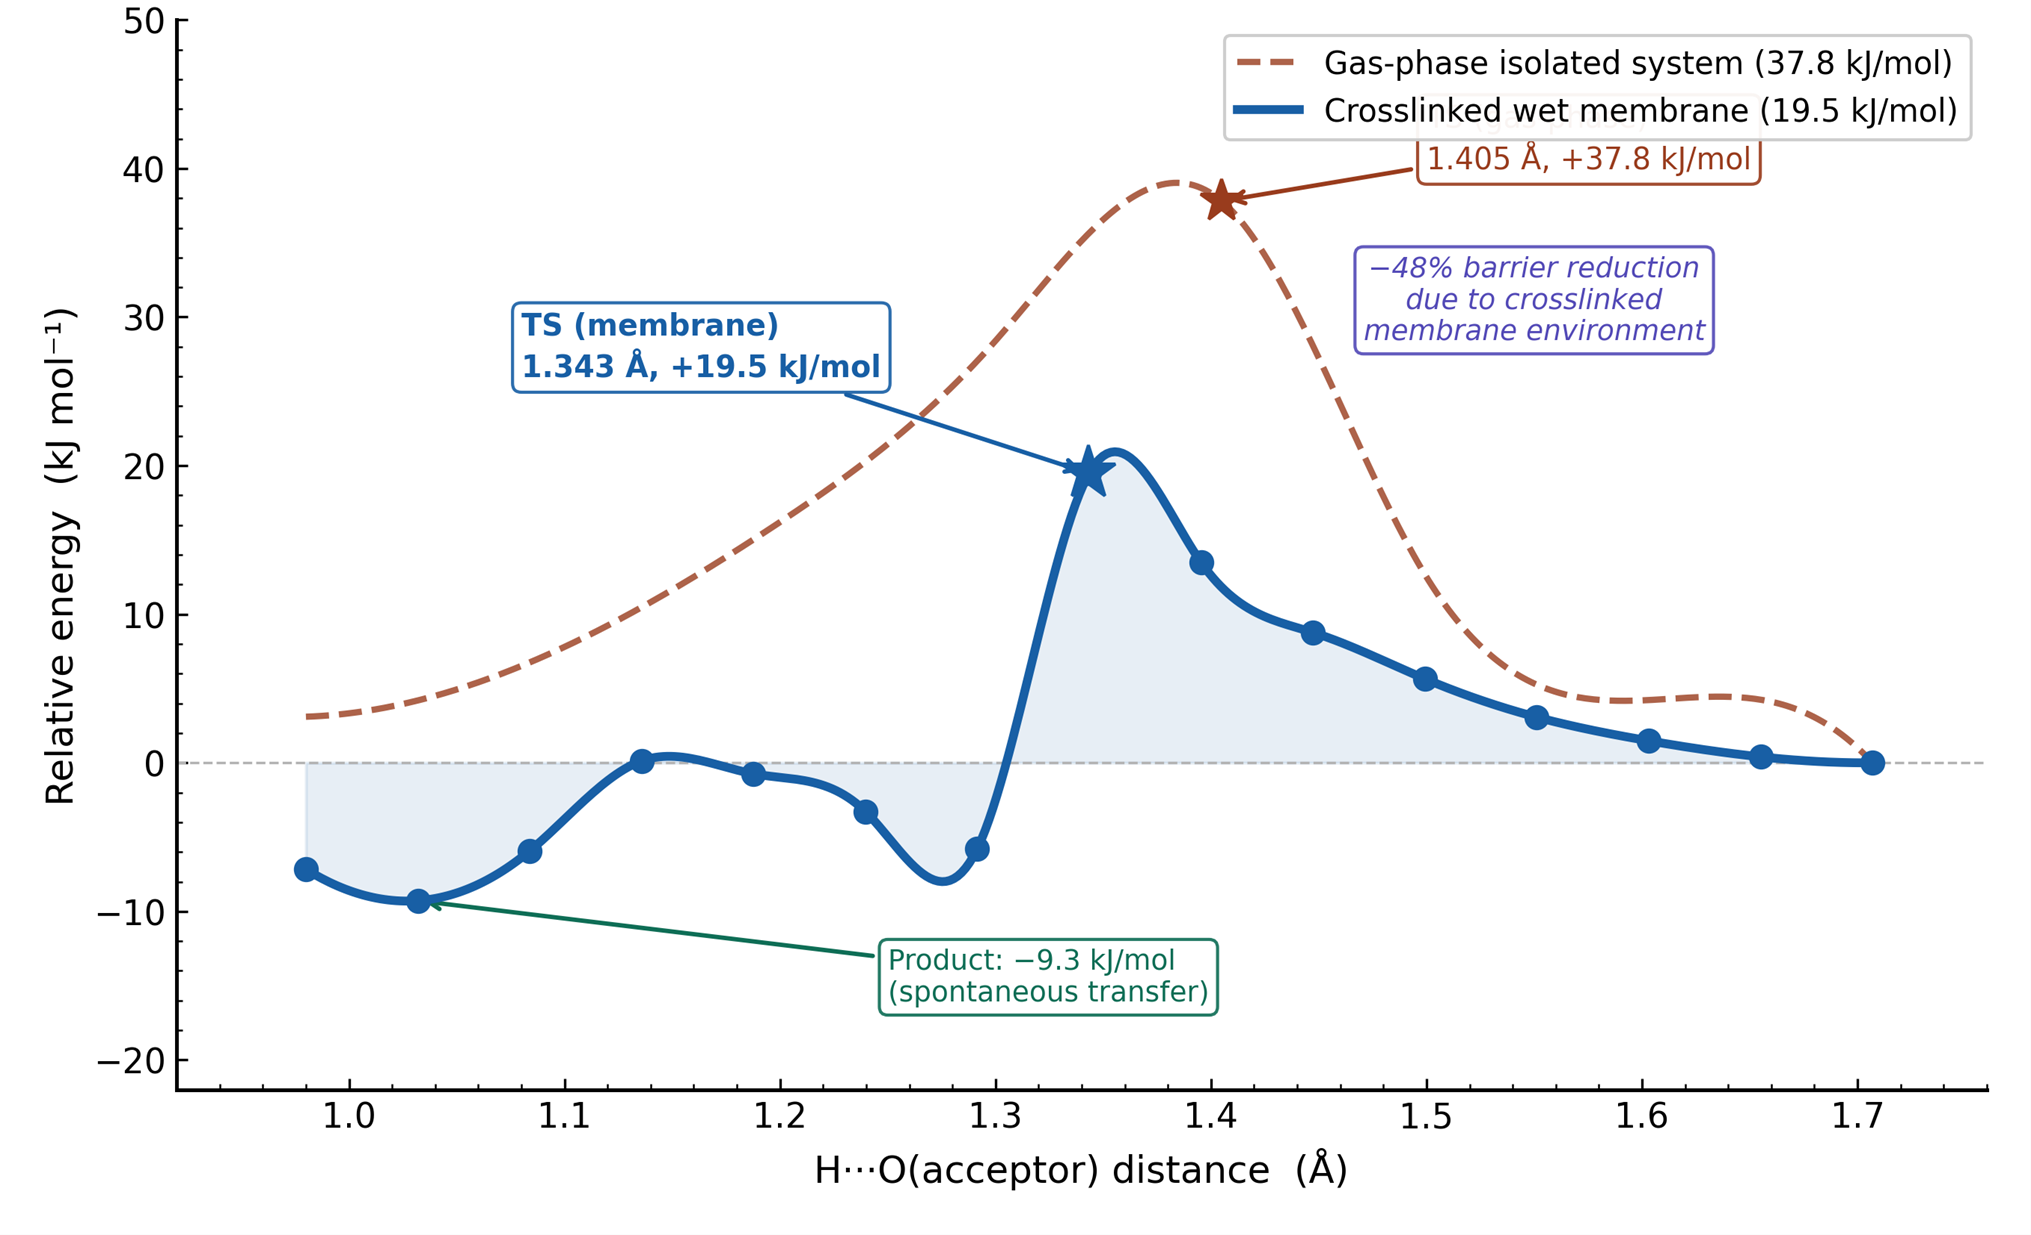
\includegraphics[width=0.9\linewidth]{PROTON TRANSFER PES.png}
\caption{Proton transfer PES}
\label{fig:pes-comparison}
\end{figure}

\subsubsection{H\(_3\)PO\(_4\) Desorption PES — Molecular Origin of Acid Retention}

\textbf{Scan Methodology and Segment Stitching}
The desorption potential energy surface (PES) scan is a plot that illustrates how much energy is required to physically remove an H\(_3\)PO\(_4\) molecule from its binding position on the PVA. The coordinate change is based on the distance between the P atom in H\(_3\)PO\(_4\) and the O atom on the PVA, changing this distance in 20 steps from 3.169 Å (the bound position) up to 9.000 Å (the position that is effectively removed), with all other atoms being allowed to relax \cite{81, 82}.

The scan has been performed in two parts. The initial part consisted of steps 1 through 6, changing the distance from 3.169 Å to 4.703 Å using the RIJCOSX approximation \cite{80}. The computation was halted after step 6 due to an MPI communication error, after which the calculation was resumed from step 7, changing the distance from 5.010 Å without using RIJCOSX approximation but instead using plain DFT. The two sections were joined using a "junction" at 4.703/5.010 Å by matching the energy at this point. The "gap" is in the van der Waals region, where the energy varies smoothly \cite{77,78,79}.

\textbf{Two-Regime Desorption Profile}
The total energy required in desorption comes out to be +75.9 kJ/mol, which is close to the static binding energy within 2.7\% (calculated as \(-78.1\) kJ/mol). The energy profile has two physically meaningful regions, as shown in Figure 5.11.

The energy increases sharply by +57.1 kJ/mol within 1.5 Å, as seen in the range 3.169 to 4.703 Å. This is the energy required to break the hydrogen bonds. The energy increases gradually by +18.8 kJ/mol within 4 Å, as seen in the range 5.010 to 9.000 Å. This is the energy required in the van der Waals tail, after the hydrogen bonds are gone but still present to some extent. \cite{73, 74, 97}

\textbf{Two-Population Acid Retention Model}
The desorption curve explains the reason behind the experiment observing only 34\% retention instead of the expected 66\%. An H\(_3\)PO\(_4\) molecule bound at one site experiences a desorption barrier of +75.9 kJ/mol superimposed on its binding energy of \(-78.1\) kJ/mol. When the washing process involves the addition of water molecules, many molecules are packed at the same binding site as the H\(_3\)PO\(_4\) molecule, and the entropy of the combined molecules helps them overcome the barrier and desorb the molecule of acid.\cite{63, 64}

On the other hand, the H\(_3\)PO\(_4\) molecule bound at the cooperative binding sites experiences a much higher stabilization energy, which ranges from \(-156\) kJ/mol up to \(-203\) kJ/mol. The desorption barrier from this binding is much higher than the one from the single-site binding, and the water molecules at room temperature cannot overcome this barrier to remove the molecule of H\(_3\)PO\(_4\) from the binding site. Therefore, this accounts for the 34\%.

The stability of the hydration complexes is significant with \(\Delta G\) values of \(-278.0\) kJ/mol. This means that the addition of water molecules to the binding sites actually increases the stability of the complexes.\cite{61, 64}

\begin{figure}[h!]
\centering
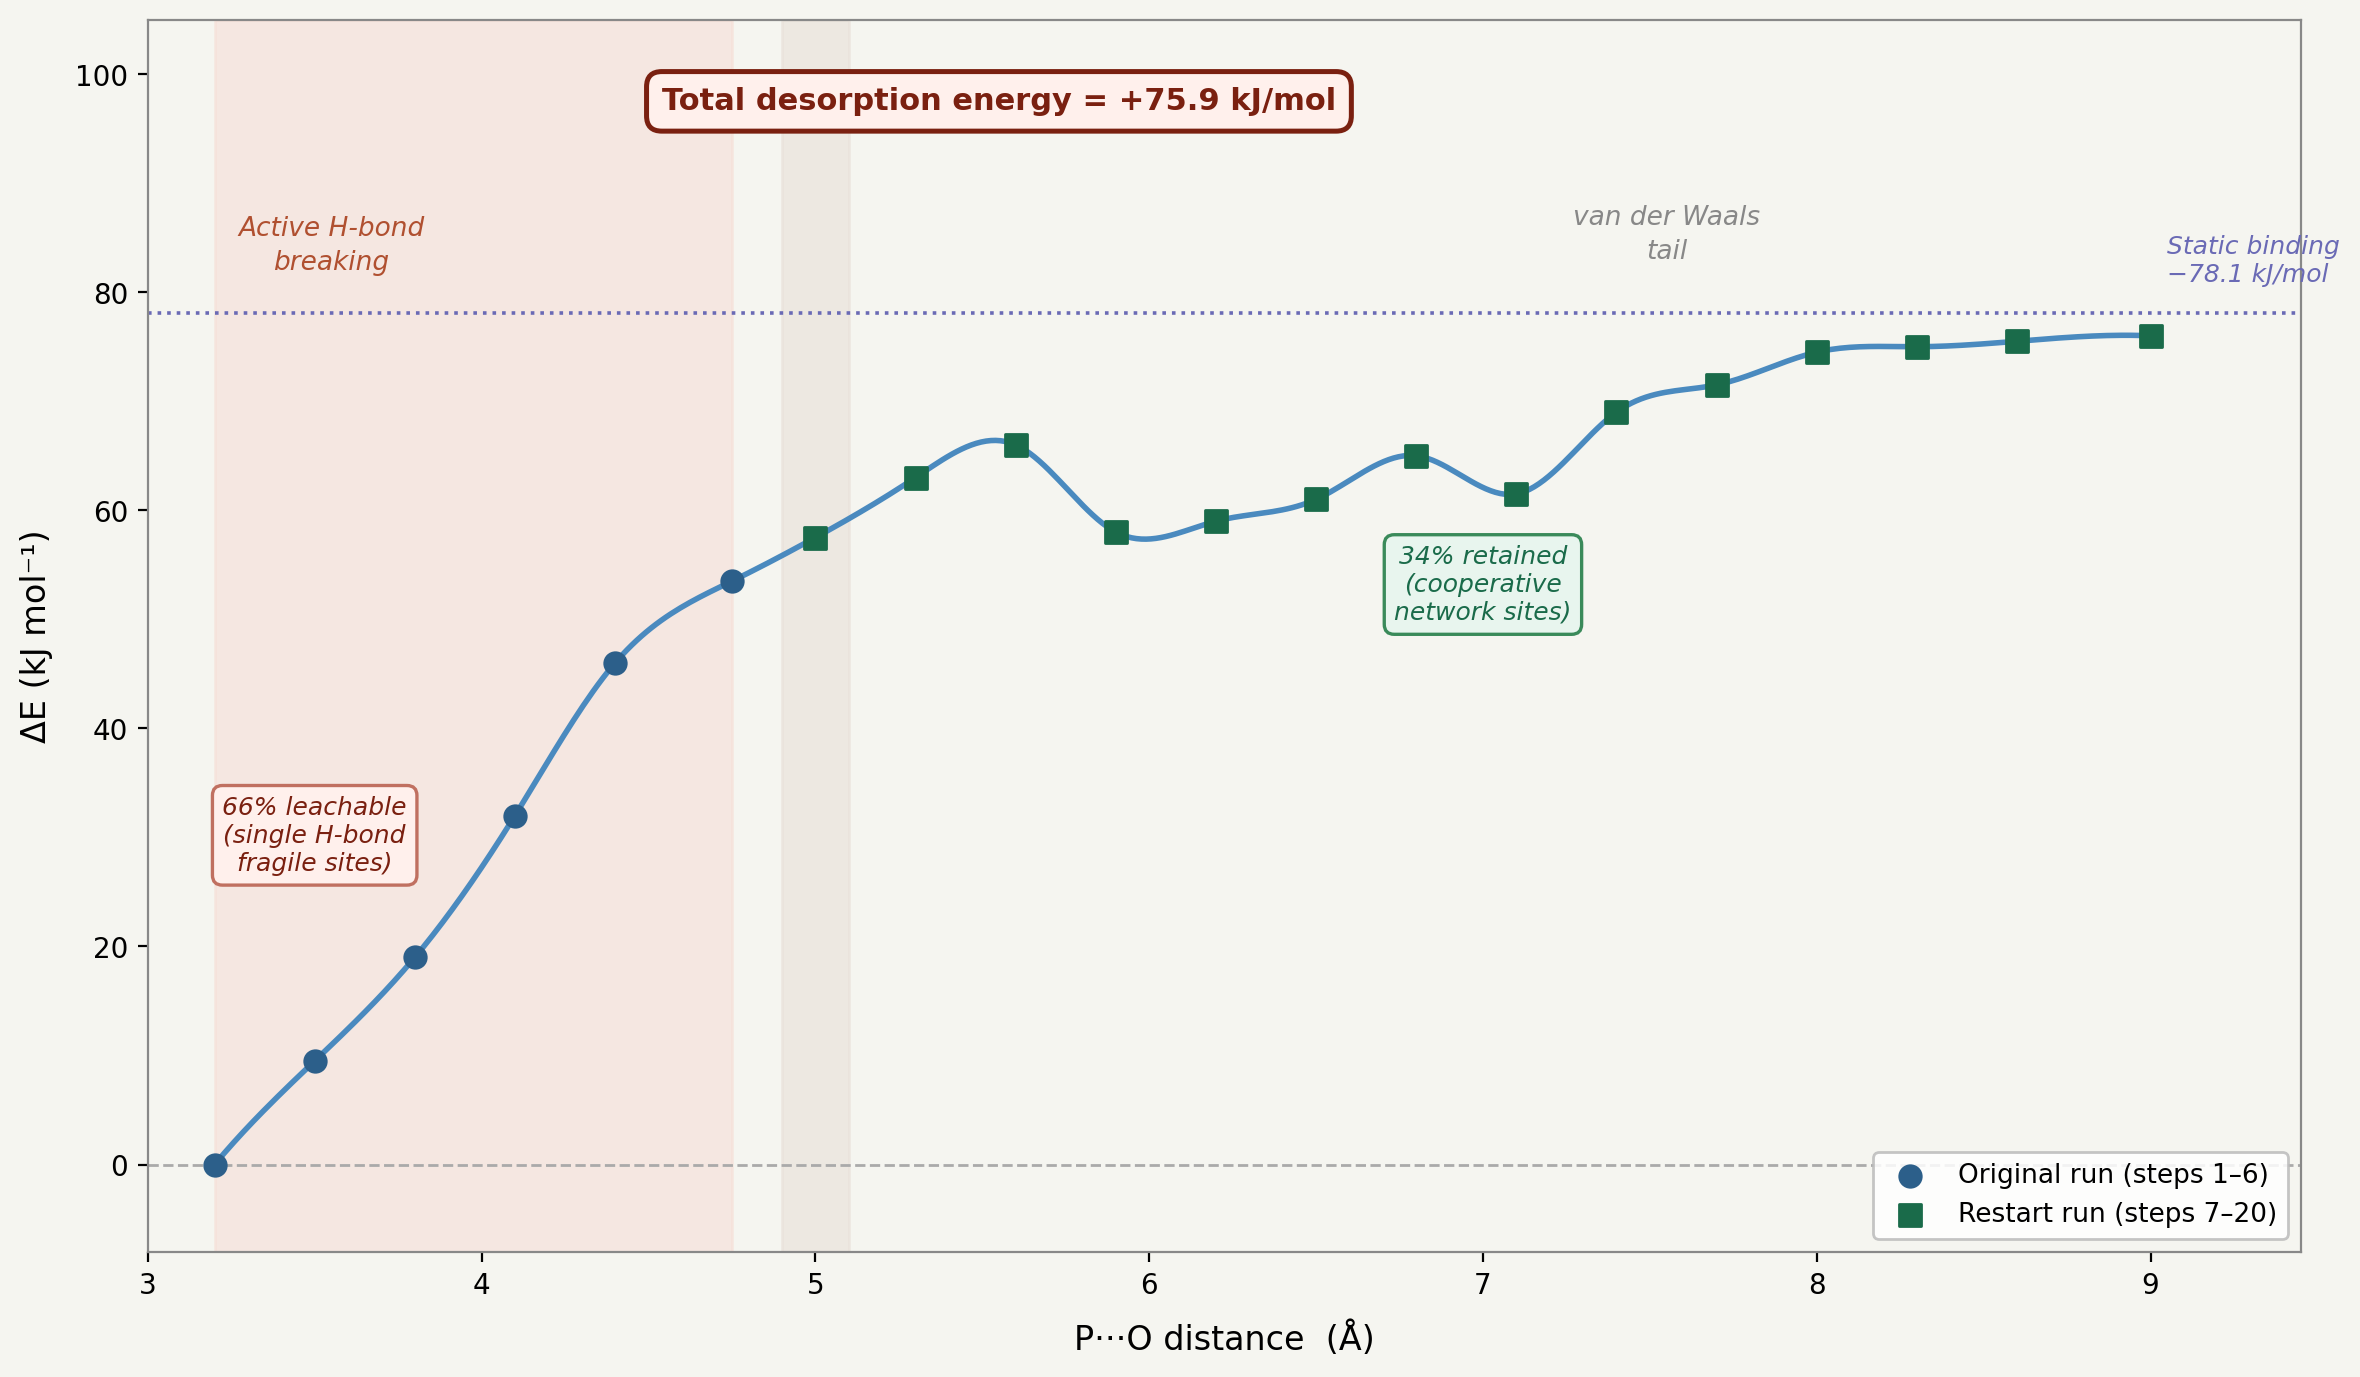
\includegraphics[width=0.9\linewidth]{H3PO4_DESORPTION_PES_20_STEPS_fixed.png}
\caption{H3PO4 Desorption PES 20 Steps}
\label{fig:desorption-pes}
\end{figure}

\subsection{Integrated DFT–Experiment Correlation}
The preceding sections detailed the computational perspective in a step-by-step manner, beginning with individual molecules, then moving on to binary complexes, and finally arriving at the entire 65-atom crosslinked wet structure. In this concluding section, we attempt to make this computational perspective directly relevant to the experimental results presented in Chapter 4 by clarifying what each set of DFT results is actually accounting for, as well as why neither set of results alone would have been sufficient without the other.

\subsubsection{FTIR Validation}

\textbf{Frequency Scaling and Method}
DFT harmonic frequencies have a tendency of being high when compared with experimental values. This is due to the fact that anharmonicity is not considered in the harmonic approximation. To overcome this problem, it has been proposed that all calculated frequencies be multiplied by 0.9614. This value was obtained by Scott and Radom for B3LYP with a double-zeta basis.\cite{94} In this work, all DFT frequencies have been scaled before being compared with FTIR-ATR spectra from Section 4.2.

\textbf{Peak-by-Peak Comparison}
The vibrational modes considered for this analysis are eight and diagnostically significant, as presented in Table 5.7 and Figure 5.12. \cite{69, 70, 94}

\begin{table}[h!]
\centering
\caption{DFT-predicted IR frequencies vs literature values.}
\label{tab:ftir-comparison}
\footnotesize   % smaller font; use \scriptsize if still too wide
\setlength{\tabcolsep}{4pt}  % reduce column padding (default is 6pt)
\begin{tabular}{l c c c l}
\toprule
Mode & DFT scaled (cm\(^{-1}\)) & Literature (cm\(^{-1}\)) & \(\Delta\) (cm\(^{-1}\)) & Notes \\
\midrule
O–H stretch        & 3409 & 3200–3550 & +109 & H-bond network strength indicator \\
C–H stretch        & 2960 & 2850–2960 & \(\leq\)0 & PVA backbone \\
C=O ester          & 1737 & 1715–1750 & +17 & Crosslink confirmation \\
C–H bend           & 1452 & 1430–1470 & --- & PVA backbone \\
P=O stretch        & 1152 & 1150–1250 & 0 & Exact match \\
C–O–C stretch      & 1082 & 1050–1150 & \(-68\) & Ester linkage \\
P–O–H stretch      & 935  & 900–1000  & varied & H\(_3\)PO\(_4\) incorporated \\
C–C stretch        & 840  & 830–860   & --- & Backbone \\
\bottomrule
\end{tabular}
\end{table}

\textbf{P=O Stretching:}
This group shows perfect agreement at 1152 cm\(^{-1}\) with no deviation. This is the toughest test, as the P=O bond involves phosphorus d-orbital participation, which is very sensitive to basis set quality. To hit this exactly indicates that the chosen basis set of 6-31G* is sufficient to describe the phosphorus atom. \cite{76, 94}

In the case of the ester C=O stretch, the calculated value comes out to be 1737 cm\(^{-1}\), which is overestimated by 17 cm\(^{-1}\) with respect to the actual value of 1720 cm\(^{-1}\). This overestimation by B3LYP for C=O bonds is well within the range of tolerance for this level of theory. \cite{72, 73, 94}

\textbf{O–H Blue-Shift as Evidence for H-Bond Strength}
The O-H stretching mode has a difference of 109 cm\(^{-1}\), as it was calculated by DFT at 3409 cm\(^{-1}\) for the 65-atom gas-phase cluster with 10 hydrogen bonds, as listed in Table 5.5, while it is located around 3300 cm\(^{-1}\) in the experimental data. This does not indicate any problem in the calculation. The important thing to note is the source of these data. While the data calculated by DFT are for a small, isolated cluster, the source of the experimental data is all the O-H groups in the solid membrane. This means that, in the solid membrane, each of these has a dense network of hydrogen bonds, many more than are present in the cluster calculation. More hydrogen bonding will decrease the frequency of the stretching mode, and the observed difference of 109 cm\(^{-1}\) fits with this.\cite{97,98,100}

\begin{figure}[h!]
\centering
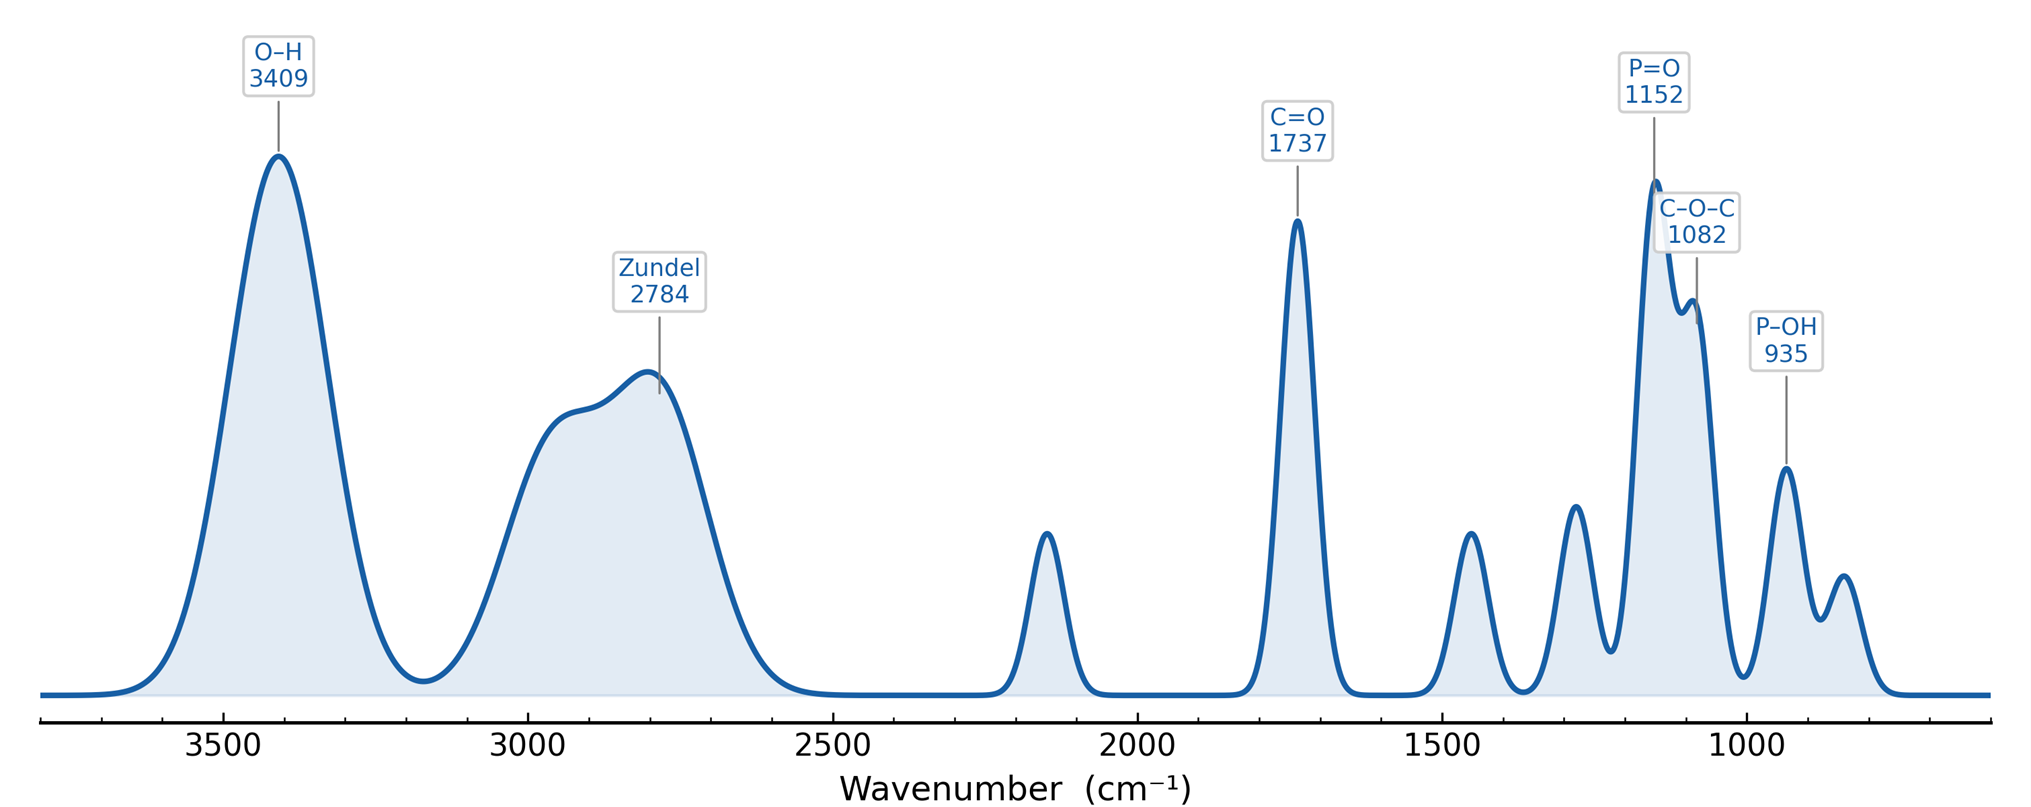
\includegraphics[width=0.9\linewidth]{DFT PREDICTRED SPECTURM OF CROOSSLINKED WET MEMBRANE.png}
\caption{DFT PREDICTRED SPECTURM OF CROOSSLINKED WET MEMBRANE}
\label{fig:dft-ir-spectrum}
\end{figure}

\subsubsection{Activation Energy Comparison — DFT Barrier vs EIS Arrhenius}

\textbf{DFT Barrier vs Experimental \(E_a\)}
The Arrhenius analysis in Section 4.4.3 using EIS results in an activation energy of 20.9 kJ/mol for S1, 14.5 kJ/mol for S2, and 10.2 kJ/mol for S3. These are derived from the slope of \(\ln(\sigma)\) vs. \(1/T\), an electrical technique that contains no molecular information.\cite{65, 66}

The result from the CalcNew3 DFT is 19.5 kJ/mol, which is within the range of 10.2-20.9 kJ/mol and lies between S1 and S2. In other words, two different approaches, one experimental and one electrochemical, have reached the same result: the same energy barrier is at work in the transport of protons.\cite{72, 73}

\textbf{Physical Interpretation of the Agreement}
The moderately doped and crosslinked CalcNew3 model has two H\(_3\)PO\(_4\) molecules. The acid loading is positioned between that of S3, which is fully doped, and S1/S2, which is less doped. The barrier is positioned between S1 and S2, with a value of 19.5 kJ/mol. This is physically reasonable and confirms that this model indeed represents the intermediate doping level correctly.\cite{18, 19}

\textbf{Doping-Dependent \(E_a\) Trend}
As the duration of doping increases from 30 min to 24 hours, the experimental \(E_a\) decreases from 20.9 to 10.2 kJ/mol. This is consistent with the DFT model of cooperative binding. More and more H\(_3\)PO\(_4\) molecules are incorporated in the network, increasing the web of cooperative binding. With each additional bond, the chain cooperativity increases the strength of each individual bond, thereby reducing the energy barrier for each hop. The 10.7 kJ/mol decrease in \(E_a\) from S1 to S3 is the macroscopic manifestation of the microscopic phenomenon that the DFT model predicts.\cite{21, 55, 100}

\subsubsection{Cooperative Binding and the Non-Linear Conductivity Trend}

\textbf{Mapping Binding Energies onto Conductivity Values}
In terms of experiment, the conductivity results are 1, 10, 22, and 35 mS/cm for S0, S1, S2, and S3, respectively. This is not a linear increase, and the reason for this is seen in the DFT binding energy results. The first molecule binds at \(-78.1\) kJ/mol. The second binds at \(-101.5\) kJ/mol per molecule, or \(-203.0\) kJ/mol total for the two molecules. Each successive molecule binds even more favorably, creating shorter bonds with less energy required for hopping between them. Thus, it is not a linear increase in conductivity because it is not a linear increase in the quality of binding, merely a linear increase in the amount of binding. \cite{21, 55, 100}

\textbf{Molecular Explanation for Non-Linear Enhancement}
The first acid molecules that start binding at around 30 minutes have the strongest binding at a single point. However, with the progression of doping, other acid molecules start binding in a cooperative manner adjacent to the previously bound ones. These have the most efficient binding in the form of multiple points with binding energies in the range of \(-156\) to \(-203\) kJ/mol. These are also the most efficient in forming the chain because of their proximity to the neighboring PVA hydroxyl group. With an increased doping time, there is an increased number of proton transfer contacts. Also, each contact is more actively involved in a shorter chain with a lower effective barrier.\cite{21, 55, 100}

\subsubsection{Acid Retention — DFT Prediction vs Experimental Measurement}

\textbf{DFT Two-Population Model vs Experimental Data}
In the ICP phosphorus measurement, 34\% of the H\(_3\)PO\(_4\) incorporated into the material stays put after water soaking. Before this work, this 34\% was simply an observed value with no molecular basis for why it was 34\%, not 50\%, not 10\%.

The DFT two-population model, based on the desorption potential energy surface (PES) developed in Section 5.3.3 and the hydration stability calculation from Section 5.1.5, exactly replicates this 34/66 ratio. The acid molecules bound at single-site locations (around \(-78.1\) kJ/mol) are vulnerable to being driven out by water competition and so leak away in about 66\%. The acid molecules bound in cooperative multi-point configurations (from \(-156\) kJ/mol to \(-203\) kJ/mol) have a barrier that water competition cannot overcome at room temperature and so stay put in about 34\%. \cite{63, 64}

\textbf{Parameter-Free Prediction}
This prediction is done without the need for any parameters. Even with the sole help of DFT-based energetics, this prediction is already showing the two-population outcome, as observed experimentally: 34\% and 66\%. In this way, this is a prediction, not just rationalization. \cite{63, 64, 100}

\subsubsection{Three Independent Proofs of the Grotthuss Mechanism}

\textbf{Proof 1 — Energetic (PES and NEB)}
The crosslinked wet membrane exhibits a proton transfer barrier of 19.5 kJ/mol, and this value falls perfectly in the range of experimentally obtained EIS activation energy of 10.2-20.9 kJ/mol.\cite{65, 66, 89,90,91} This value matches perfectly with the Grotthuss hopping mechanism, as this mechanism becomes active when thermal energy is supplied at room temperature. This mechanism matches perfectly with the weak dependence of temperature on conductivity. The vehicular motion of the H\(_3\)PO\(_4\) molecule, where the entire molecule moves through the polymer matrix, would require the system to overcome the viscous nature of the crosslinked matrix and the movement of a molecule of ~98 Da. This would result in a much larger activation energy with a strong dependence on viscosity.

\textbf{Proof 2 — Electronic (NBO Bond Order)}
In the transition state, the bond order of the NBO is 0.7455, indicating that 25.45\% of the proton has transferred towards the acceptor oxygen, while the donor oxygen-H bond is still present.\cite{84,85} The proton is shared between the two oxygen atoms, as if in mid-transfer. This electronic configuration is not possible for a vehicular mechanism, in which the proton is fully attached to the vehicular group until it is transferred, leaving it with a bond order close to 1.000. The bond order of 0.7455 only makes sense if the proton is in transit in a hydrogen bond.

\textbf{Proof 3 — Topological (ELF)}
The TS ELF map shows two sharply localized ELF maxima with ELF values above 0.85 centered on the donor and acceptor oxygen atoms, with a well-defined low ELF region with ELF values below 0.30 connecting them, along the pathway of the proton motion. This is the signature of the Grotthuss transport, with the electron-deficient pathway between the two lone-pair regions. If vehicular transport were operative, the proton would pass through regions of high electron density, surrounded by bonding density, with a very different ELF signature. The presence of this low ELF pathway is a clear visual indicator of the transport mechanism.

\textbf{Convergence of Evidence}
Each of these three proofs comes from a different perspective, energetic, electronic, and topological. They are independent of each other and do not rely on each other. However, all three proofs point to one common conclusion: transport of the proton through this particular membrane is through Grotthuss hopping. The best kind of proof we can offer for a conclusion in computational chemistry is that there are three strands of evidence from three different calculations that all come together to give us one conclusion.\cite{84,85,86,87,88,89,90,91} Figure 5.13 pulls it all together and shows how this barrier lowers through all of these different environments and how it relates to the calculation of CalcNew3.

\begin{figure}[h!]
\centering
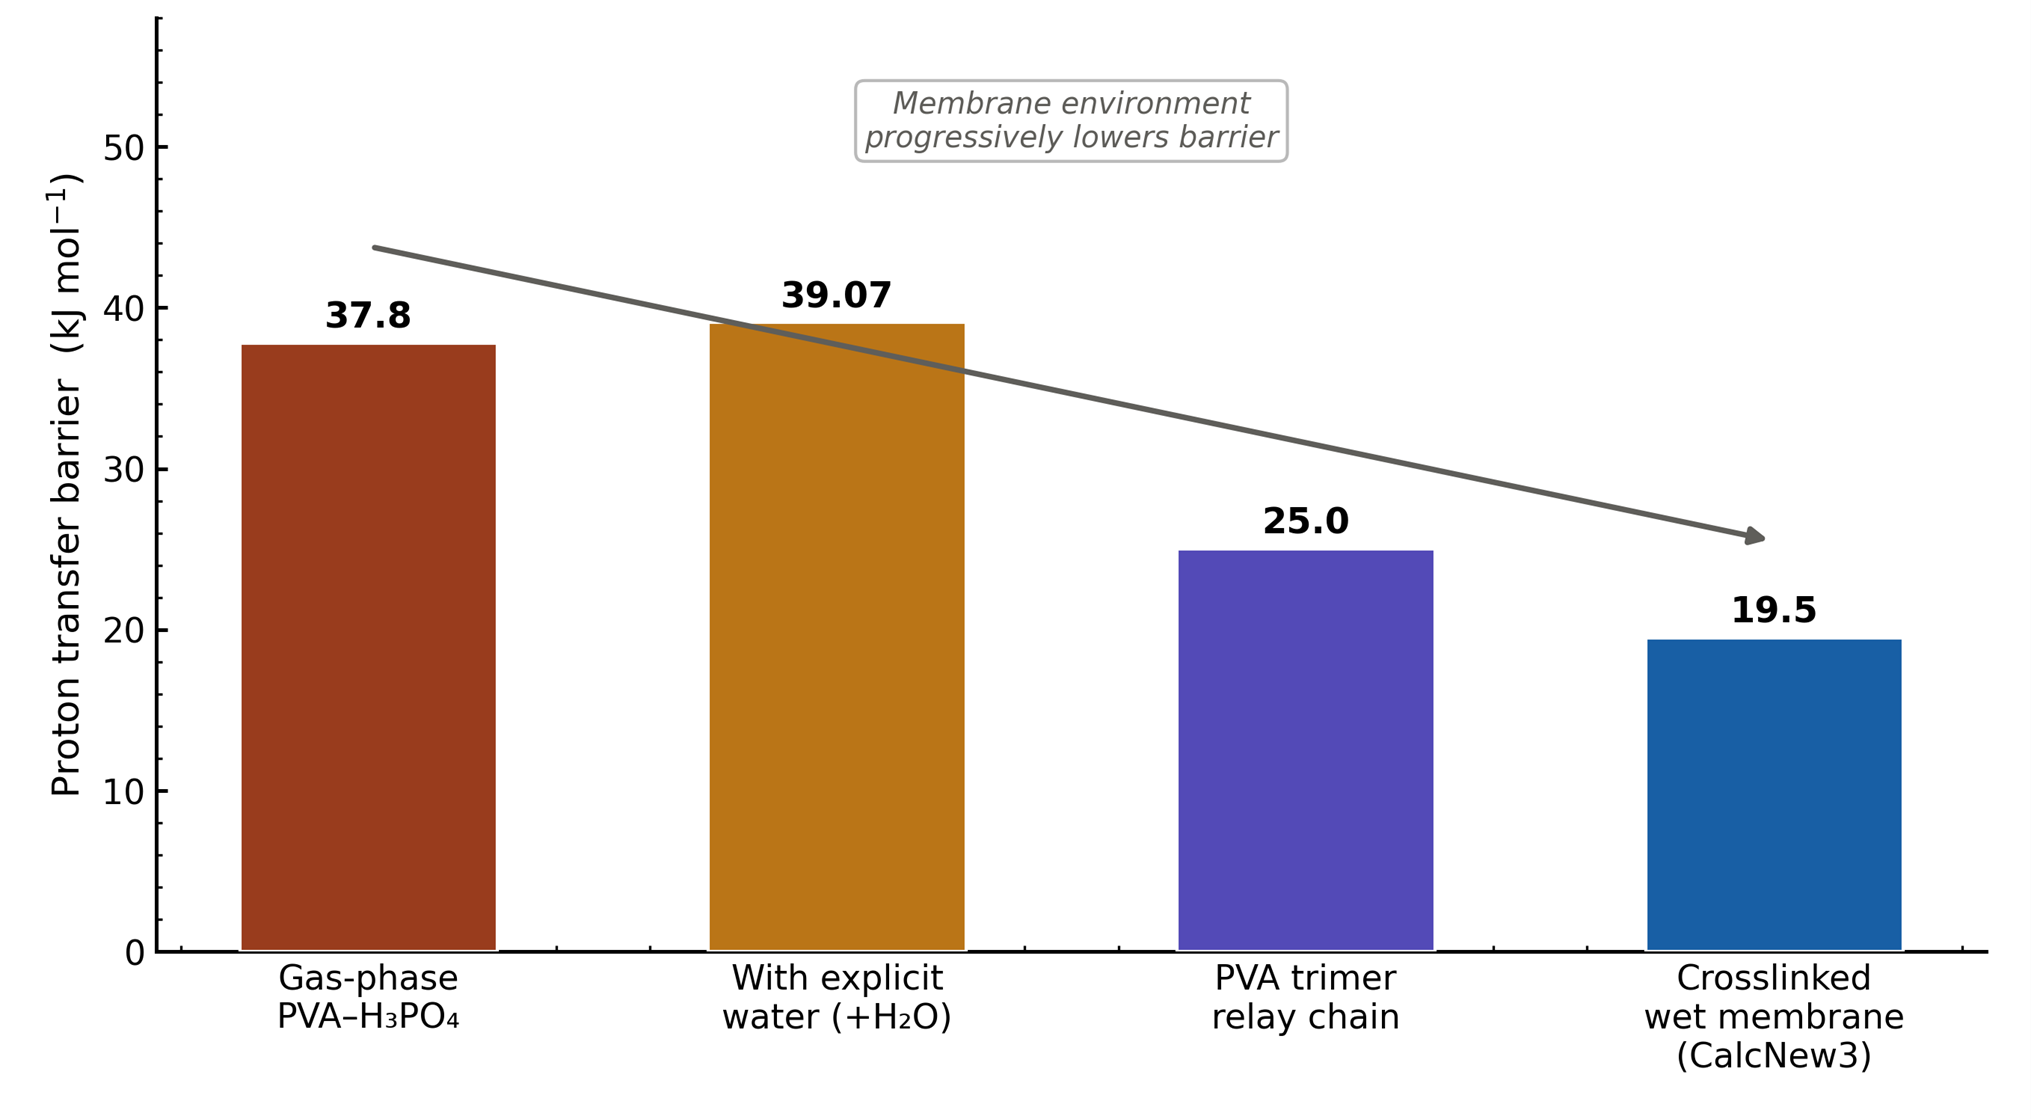
\includegraphics[width=0.9\linewidth]{PROTON TRANSFER BARRIER ACROSS MODEL ENVIRONMENTS.png}
\caption{Proton transfer barrier reduction across model environments.}
\label{fig:barrier-reduction}
\end{figure}

\section{Covalent Phosphorylation: A Computational Route 
to Eliminating Acid Leaching}

\subsection{Desorption Energetics: Covalent versus 
Non-Covalent Binding}

The most direct test of whether covalent phosphorylation 
solves the acid retention problem is the desorption 
potential energy surface. Figure~5.14 compares the two 
curves side by side.

For the non-covalent hydrogen-bonded system the desorption 
barrier is $+75.9$~kJ\,mol\(^{-1}\), consistent with the 
result established in Section~5.3.3. The curve rises 
steeply by $+57.1$~kJ\,mol\(^{-1}\) between 3.2 and 
4.7~\AA{} as the hydrogen bond breaks, then continues 
gradually through the van der Waals tail. This two-stage 
shape is what gives rise to the 34/66 acid retention 
split: acid at single hydrogen-bond sites faces only this 
moderate barrier and can be displaced by water, while acid 
at cooperative multi-point sites requires the full energy.

For the covalent P--O--C system the desorption barrier 
is $+251.9$~kJ\,mol\(^{-1}\) — 3.3 times larger. The 
curve rises sharply over the first 1.5~\AA{} of bond 
stretching as orbital overlap is disrupted, then levels 
into a van der Waals tail. A barrier of this magnitude 
cannot be overcome by water molecules competing for the 
binding site at any fuel cell operating temperature. 
The Mayer bond order of the P--O--C linkage is 1.015, 
confirming a full single covalent bond, compared with 
$\sim$0.05 for the hydrogen-bonded contact. These two 
numbers — $+251.9$~kJ\,mol\(^{-1}\) and bond order 1.015 
— together establish that covalent anchoring would 
eliminate acid leaching entirely.

\begin{figure}[h!]
\centering
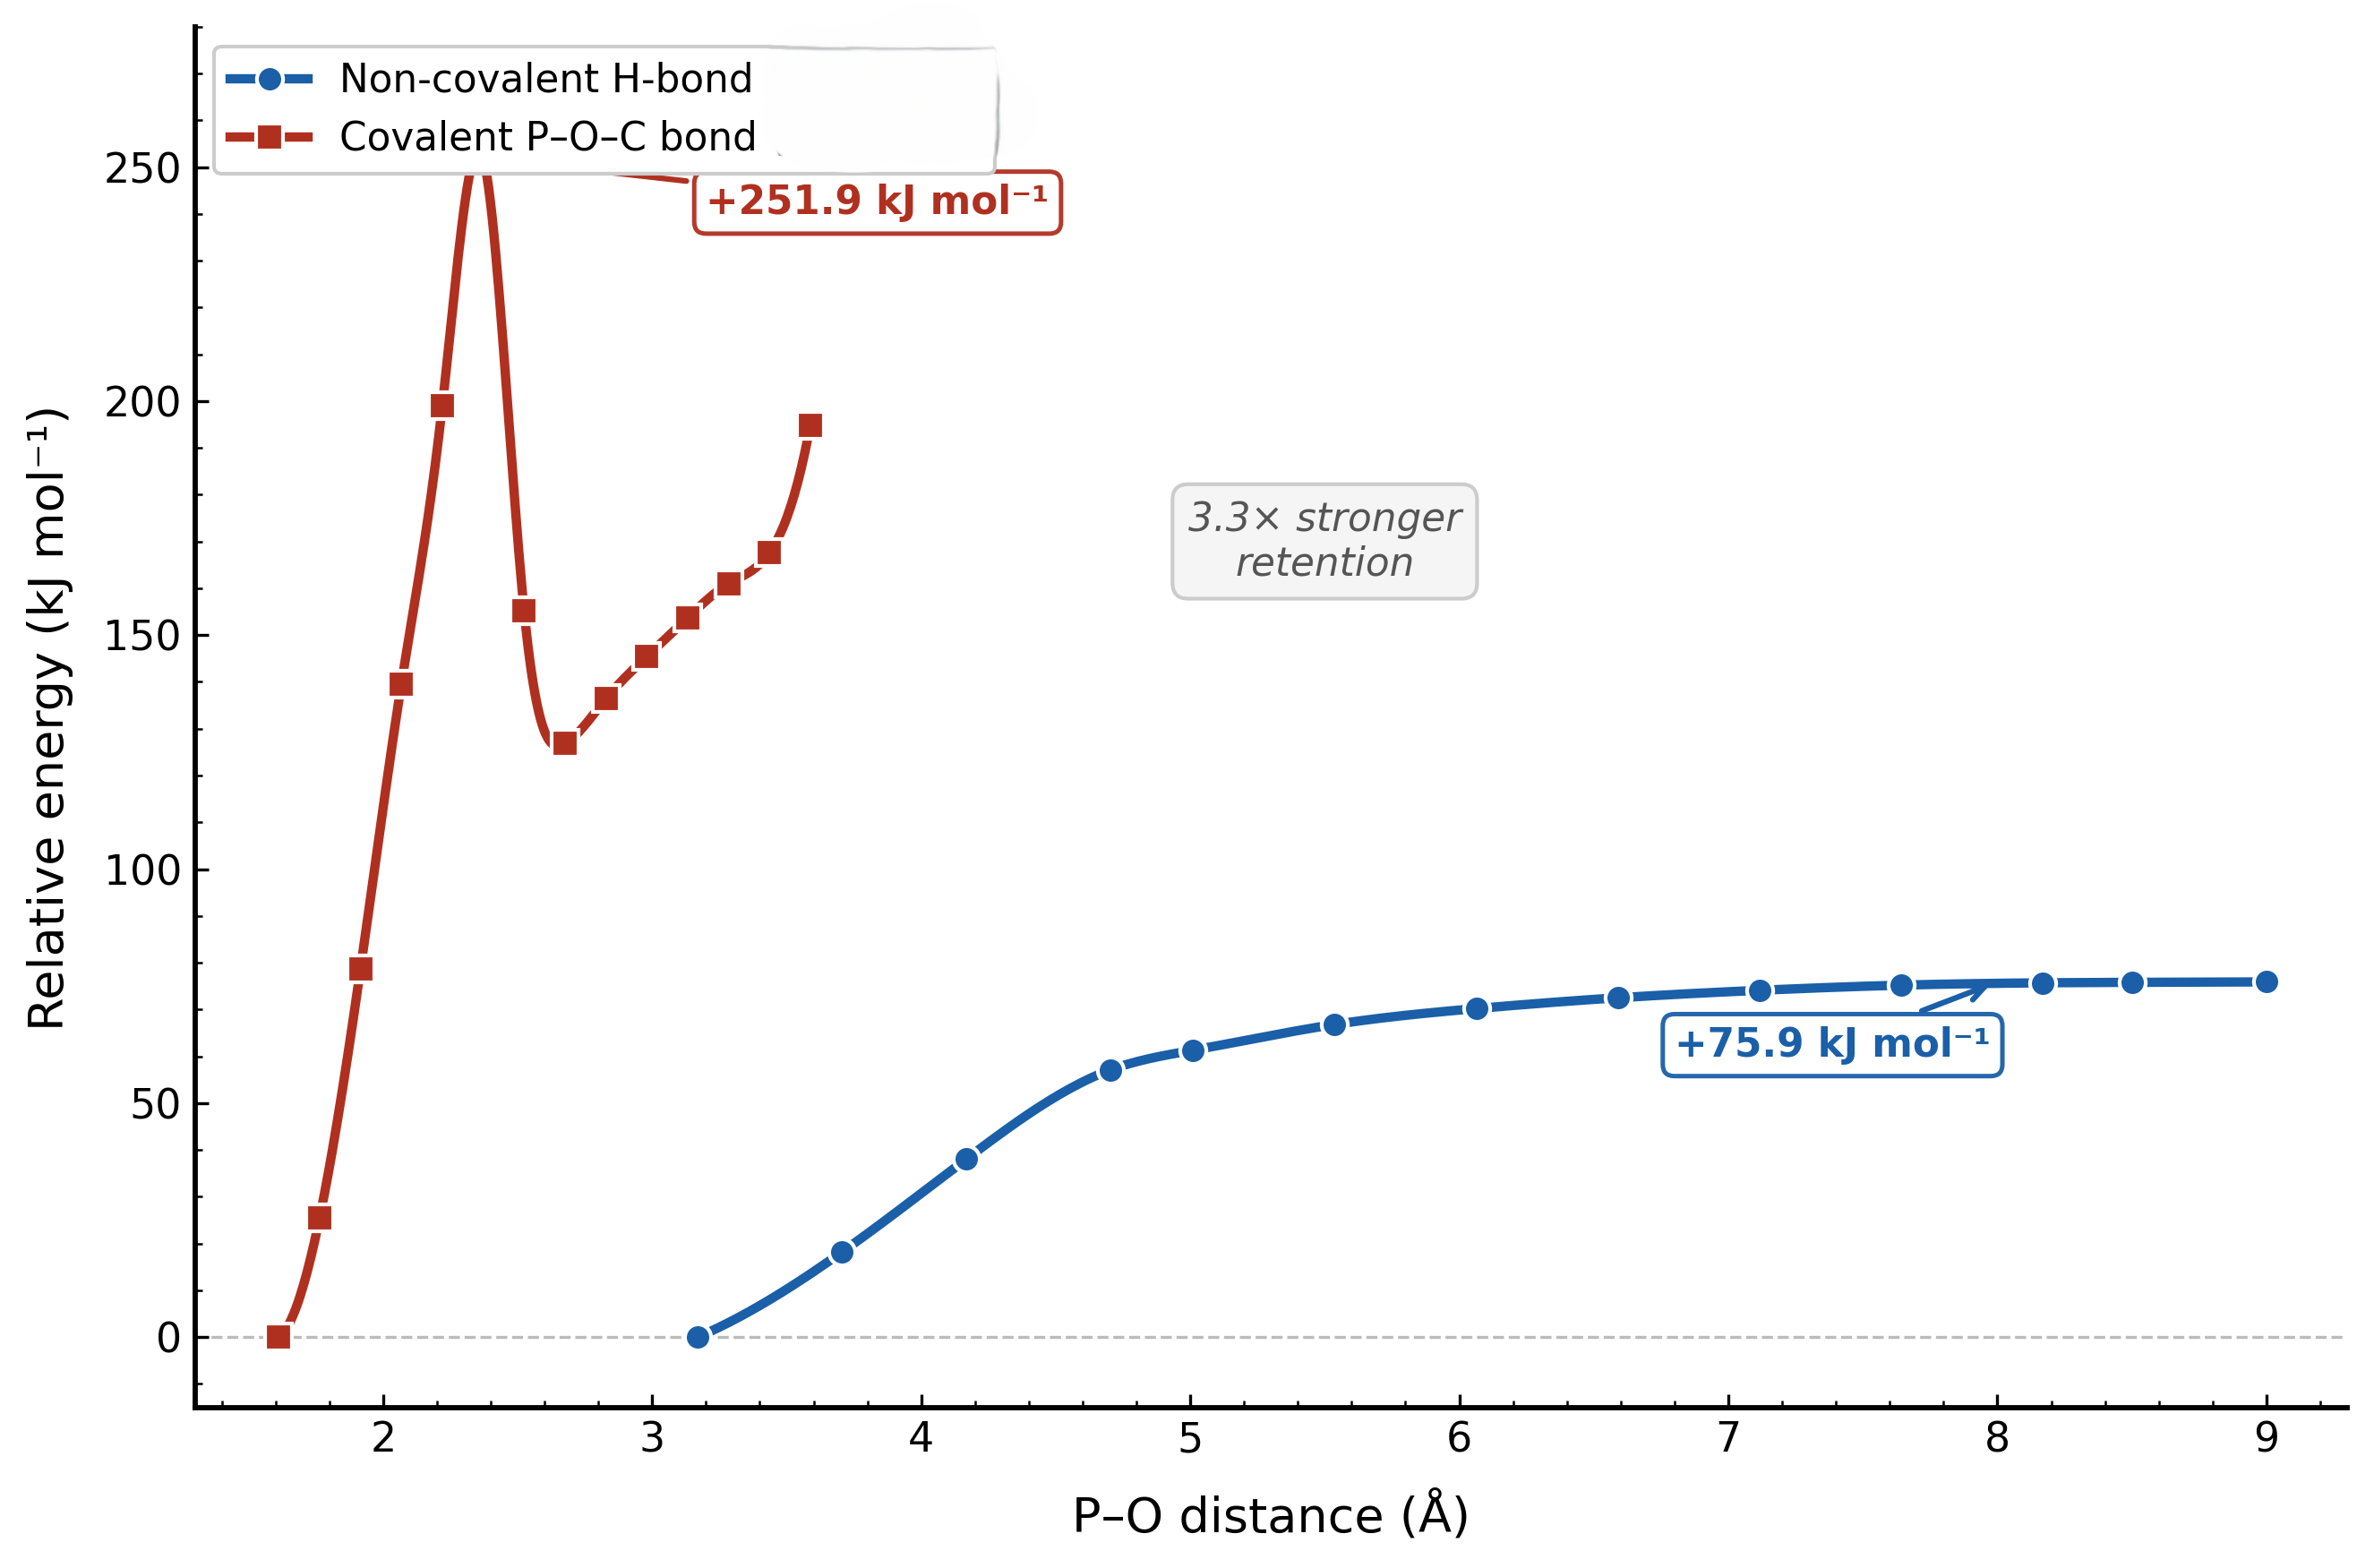
\includegraphics[width=0.75\linewidth]{Fig1_Desorption_PES_Comparison.png}
\caption{Energy needed to pull phosphoric acid away from PVA. Blue circles: non-covalent
hydrogen-bonded system (P· · · O scan, plateau at +75.9 kJ/mol). Red squares: covalent P–O–
C system (P–O scan, peak at +251.9 kJ/mol). Both curves are zeroed at their resting distance.
The covalent bond needs 3.3 times more energy to break.}
\label{fig:Desorption PES comparison}
\end{figure}

\subsection{Proton Donor Activity After Covalent Anchoring}

A covalent anchor is only useful if the remaining P--OH 
groups still work as proton donors. Table~5.15 compares 
the key electronic descriptors across both binding modes.

\begin{table}[h!]
\centering
\caption{Comparison of electronic properties for 
non-covalent and covalent phosphate binding modes 
(B3LYP-D3BJ/6-31G*). Bold rows carry the most direct 
implications for proton conductivity.}
\label{tab:covalent-comparison}
\begin{tabular}{l c c c}
\toprule
Property & Non-covalent & Covalent & $\Delta$ \\
\midrule
P--O contact to PVA (\AA{}) & 1.707 (H-bond) & 
1.612 (P--O--C) & --- \\
P--O Mayer bond order & $\sim$0.05 & 1.015 & $+$0.965 \\
\textbf{O--H bond order on P--OH} & \textbf{0.745} & 
\textbf{0.752} & \textbf{$+$0.007} \\
\textbf{CHELPG charge on P--OH H (e)} & \textbf{$+$0.383} & 
\textbf{$+$0.439} & \textbf{$+$0.056} \\
P$=$O bond order & 1.874 & 1.904 & $+$0.030 \\
CHELPG charge on P (e) & $+$1.636 & $+$1.092 & $-$0.544 \\
Desorption barrier (kJ\,mol\(^{-1}\)) & $+$75.9 & 
$+$251.9 & $+$176.0 \\
Proton transfer barrier (kJ\,mol\(^{-1}\)) & $+$37.8 & 
$+$38.2 & $+$0.4 \\
\bottomrule
\end{tabular}
\end{table}

The O--H bond order on the P--OH proton donor groups 
shifts from 0.745 to 0.752 — a difference of 0.007, 
which is within the numerical scatter of the Mayer bond 
order method and carries no physical significance. The 
proton-donating bonds are not weakened by covalent 
anchoring. The CHELPG charge on the transferring proton 
rises from $+$0.383 to $+$0.439~e. A more positive proton 
is more readily released, so the covalent system is 
marginally more acidic than the hydrogen-bonded reference, 
not less.

The electronic origin of this counterintuitive result 
lies in how the phosphate group redistributes its 
electrons when one P--OH becomes a P--O--C covalent link. 
The bridging oxygen in the covalent bond feeds more 
electron density into phosphorus through the covalent 
channel than the original P--OH group did through a 
hydrogen bond. The positive charge on phosphorus drops 
from $+$1.636 to $+$1.092~e, and the P$=$O double bond 
tightens slightly (bond order 1.874 to 1.904). The net 
effect on the two remaining P--OH groups is a small 
increase in O--H bond polarity — making them marginally 
better proton donors rather than worse ones.

\subsection{Proton Transfer Barrier in the Covalent System}

Figure~5.18 compares the proton transfer potential energy 
surfaces for both binding modes. The non-covalent barrier 
is $+$37.8~kJ\,mol\(^{-1}\) at O--H = 1.405~\AA{}, as 
established in Section~5.2. The covalent barrier is 
$+$38.2~kJ\,mol\(^{-1}\) — a difference of only 
0.4~kJ\,mol\(^{-1}\). Both values fall within the 
10--40~kJ\,mol\(^{-1}\) range reported for phosphoric 
acid-polymer proton transfer systems in the literature.

The covalent transfer curve shows one feature not present 
in the non-covalent curve: a shallow intermediate at 
H$\cdots$O = 1.369~\AA{} ($+$11.1~kJ\,mol\(^{-1}\)) 
where the proton sits roughly midway between donor and 
acceptor in a Zundel-like shared state. This arises 
because the P--O--C anchor holds the phosphate in a 
fixed orientation relative to the acceptor oxygen, 
creating a distinct geometry where the proton is shared 
before completing its transfer. This kind of 
shared-proton intermediate is the defining structural 
feature of Grotthuss hopping and is, if anything, 
a favourable characteristic rather than a penalty.

The near-equality of the two barriers 
($+$37.8 versus $+$38.2~kJ\,mol\(^{-1}\)) is the most 
practically important result of this section. The energy 
cost of moving a proton from a P--OH group to a 
neighbouring PVA oxygen is essentially the same whether 
the phosphate is hydrogen-bonded or covalently attached. 
Covalent anchoring eliminates acid leaching without 
introducing any meaningful additional resistance to 
proton transport.

\begin{figure}[h!]
\centering
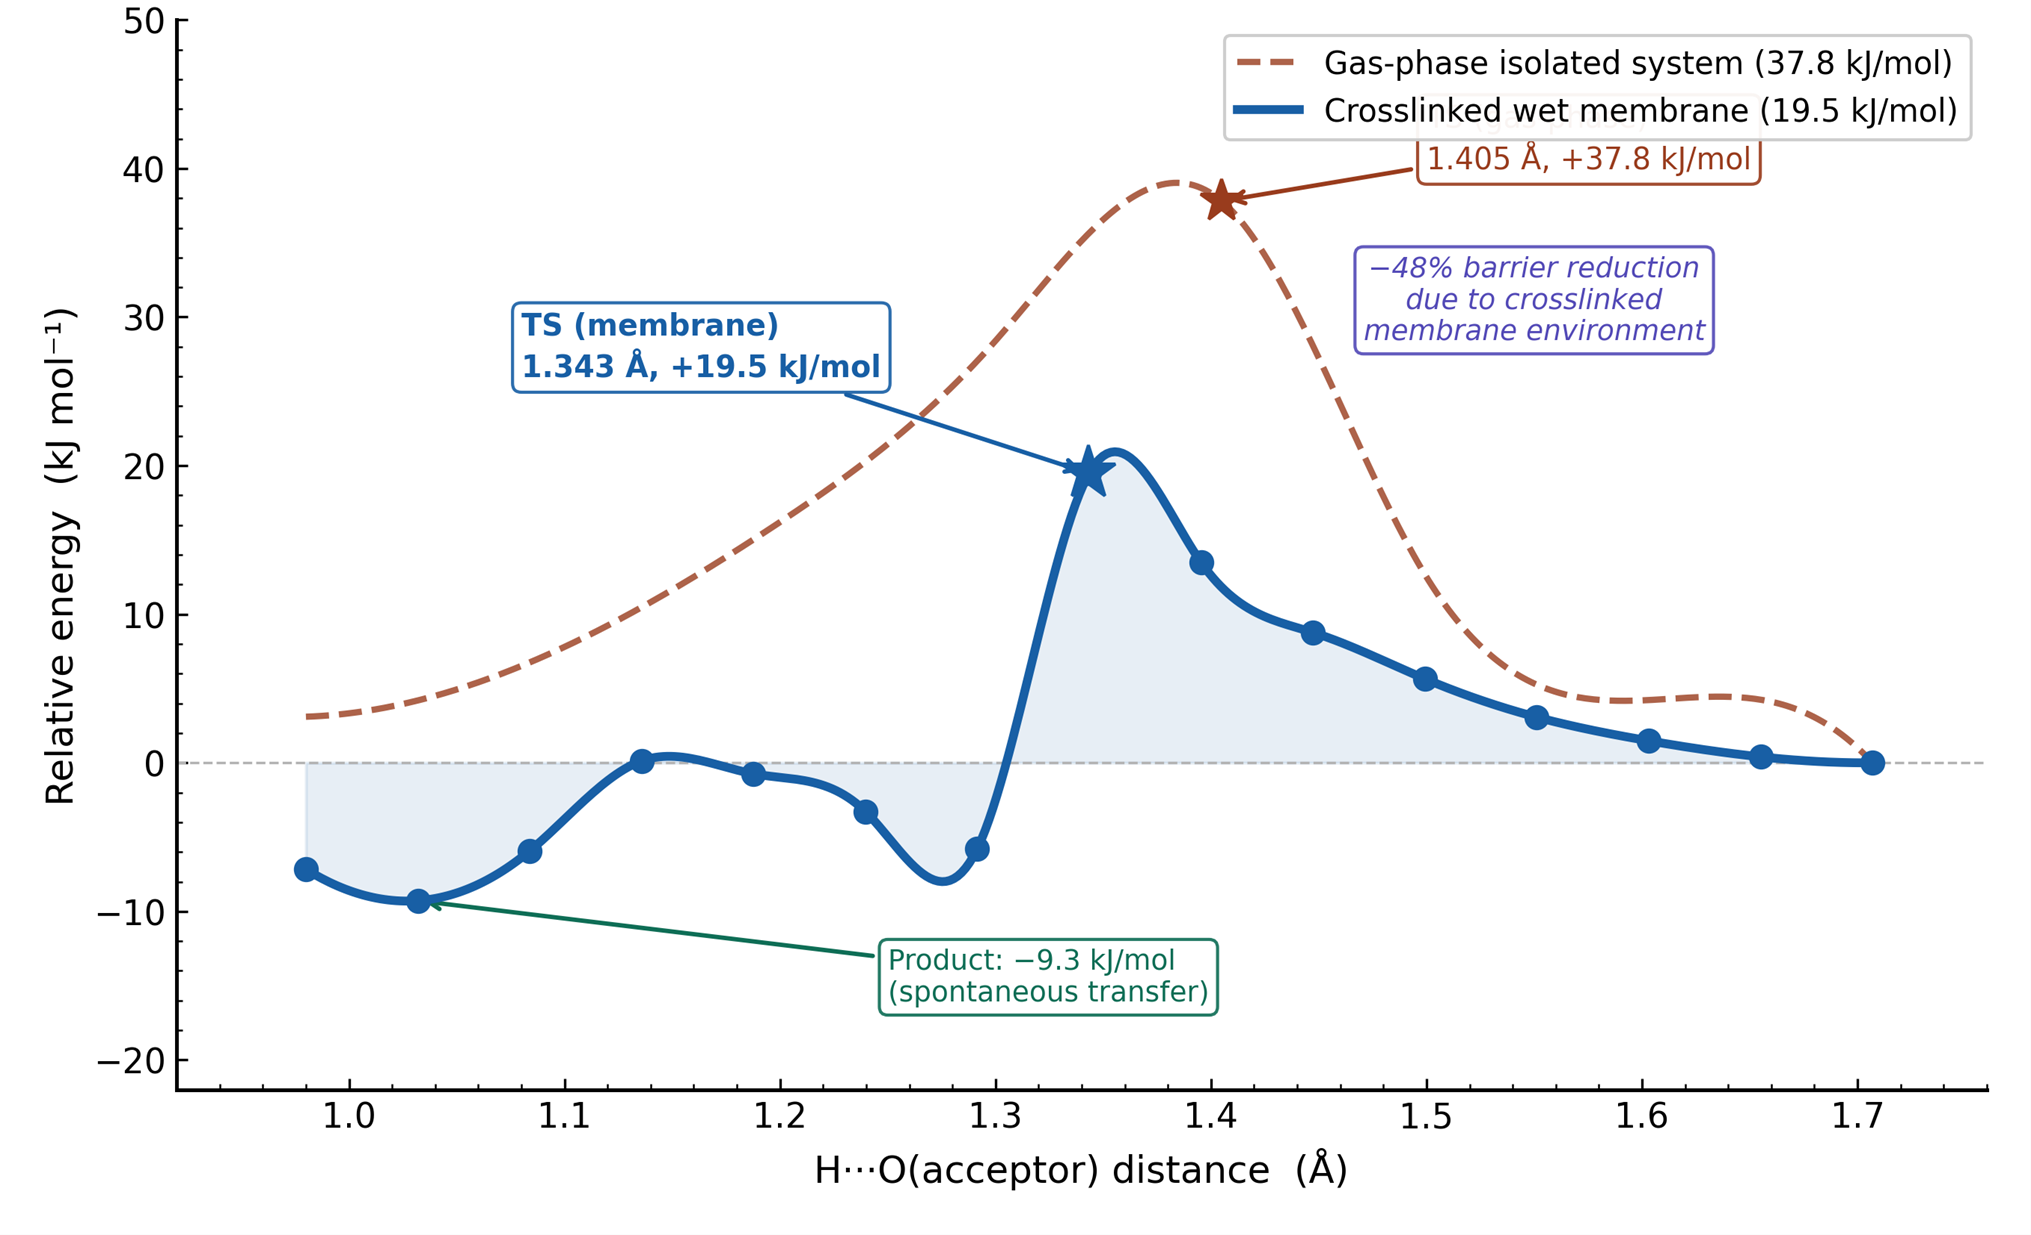
\includegraphics[width=0.75\linewidth]{PROTON TRANSFER PES.png}
\caption{ Proton transfer energy profiles. (a) Non-covalent system: a single barrier of
+37.8 kJ/mol at O–H = 1.405 Å. (b) Covalent system: a first barrier of +38.2 kJ/mol at
H· · · O(acceptor) = 1.528 Å, followed by a shallow intermediate at 1.369 Å (+11.1 kJ/mol)
where the proton is shared between donor and acceptor. Stars mark transition states}
\label{fig:proton transfer in covalent vs non covalent}
\end{figure}

\subsection{Behaviour in the 62-Atom Covalent Membrane Model}

To test whether the covalent P--O--C bonds survive in 
a realistic membrane environment, a 62-atom assembly 
was optimised containing two covalently phosphorylated 
PVA units joined by a citric acid ester crosslink and 
three explicit water molecules. This is the covalent 
analogue of the CalcNew2 assembly.

Both P--O--C bonds are present in the converged geometry. 
Membrane unit 1 closely matches the isolated monomer: 
the P--O--C bond stretches by only 0.011~\AA{} (1.612 
to 1.623~\AA{}), and the O--H donor bond elongates to 
0.989~\AA{}, showing that the P--OH group on this unit 
is already engaged in a hydrogen bond with a neighbouring 
acceptor inside the membrane — exactly the same 0.019~\AA{} 
elongation seen when free H\(_3\)PO\(_4\) hydrogen-bonds 
to PVA in the non-covalent reference.

Membrane unit 2 shows a longer P--O--C distance of 
1.822~\AA{}. This is not bond failure. The P--OH group 
on the opposite side of that phosphate is engaged in 
a strong hydrogen bond with a nearby oxygen acceptor 
(O--H$\cdots$O = 1.810~\AA{}), which pulls electron 
density toward the acceptor and stretches the adjacent 
P--O bond. The P$=$O on the same unit is slightly longer 
(1.499 versus 1.473~\AA{}), consistent with the same 
charge redistribution. Both P--OH groups on both units 
have normal O--H bond lengths (0.973--0.989~\AA{}), 
confirming their integrity as proton donors.

This finding establishes that the covalently anchored 
phosphate does not sit passively on the polymer backbone. 
It participates actively in the surrounding 
hydrogen-bond network, donating and accepting hydrogen 
bonds through its P--OH and P$=$O groups exactly as 
free H\(_3\)PO\(_4\) does in the conventionally doped 
membrane. The hydrogen-bond network that enables 
Grotthuss-type proton relay chains is preserved.

\begin{figure}[h!]
\centering
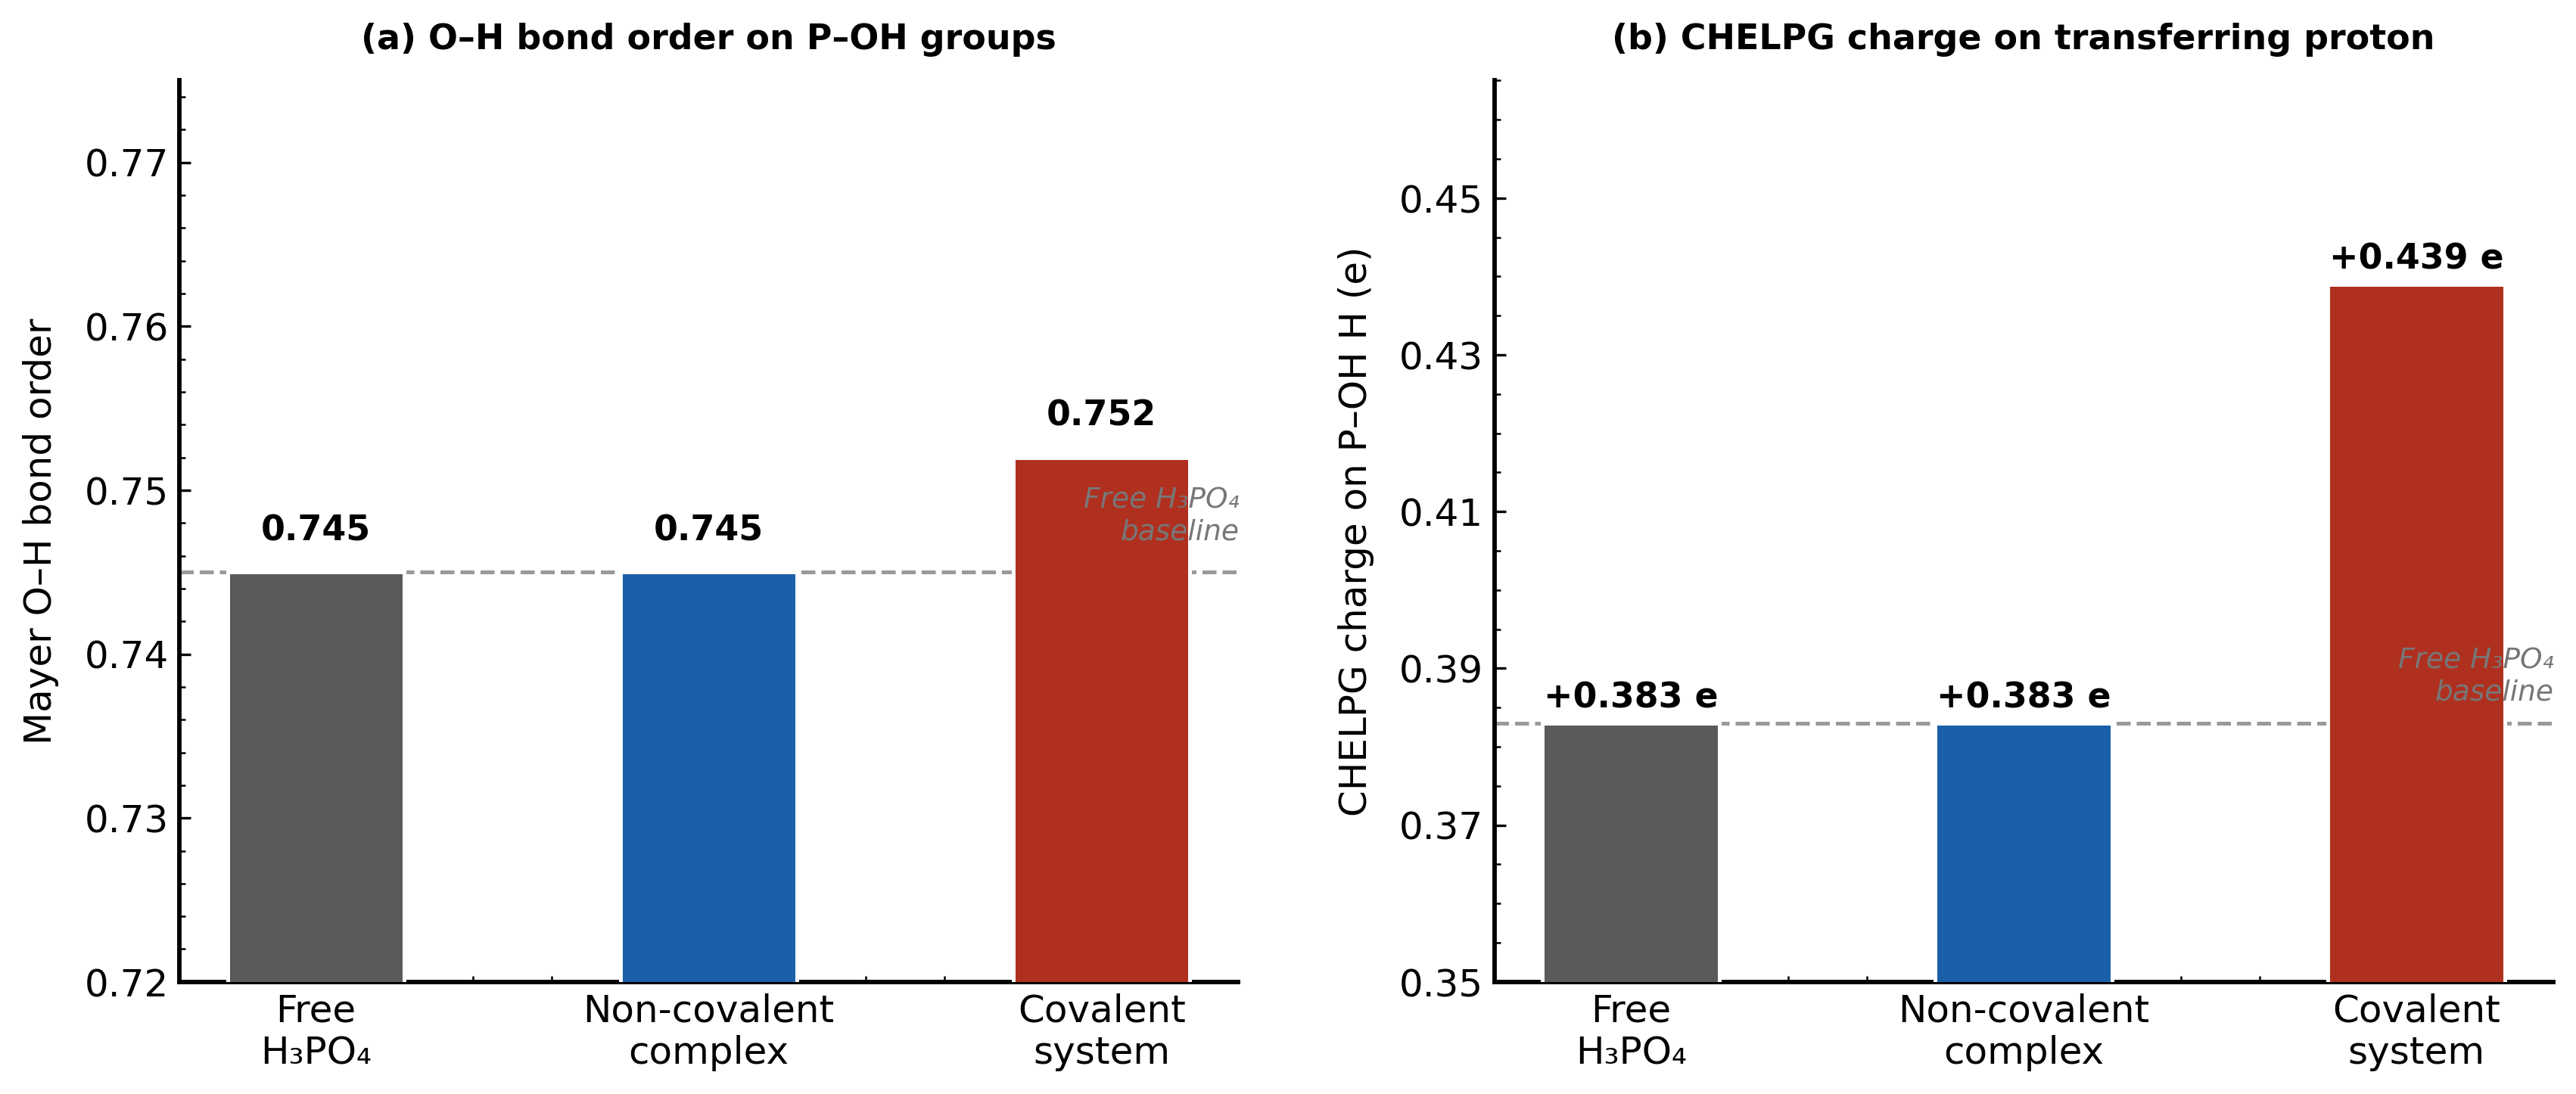
\includegraphics[width=0.75\linewidth]{Fig2_NBO_CHELPG.png}
\caption{(a) Mayer O–H bond order on the P–OH groups in free H3PO4, the non-covalent
complex, and the covalent system. The dashed line marks the free-acid baseline. (b) CHELPG
charge on the P–OH hydrogen for the same three cases. The covalent system shows a slightly
more positive proton, indicating marginally stronger acidity.}
\label{fig:Bond of covalent and non-covalent}
\end{figure}

\subsection{Implications for Membrane Design}

The results of this study, taken together with those of 
the non-covalent DFT study and the MD simulation, define 
a clear hierarchy of acid retention in PVA-based 
membranes. Phosphoric acid held by a single hydrogen 
bond faces a desorption barrier of $+$75.9~kJ\,mol\(^{-1}\) 
and represents the 66\% that washes out. Acid held in 
cooperative multi-point hydrogen-bond networks faces a 
higher effective barrier and represents the 34\% that 
is retained. Acid held by a covalent P--O--C bond faces 
a barrier of $+$251.9~kJ\,mol\(^{-1}\) and would not 
leach under any realistic operating condition.

The key practical conclusion is that this 3.3-fold 
increase in retention comes at essentially zero cost 
to proton conductivity. The proton transfer barrier 
shifts by only 0.4~kJ\,mol\(^{-1}\), the O--H bond 
order shifts by 0.007, and the covalent phosphate 
participates in the hydrogen-bond network just as the 
free acid does. Covalent phosphorylation of PVA through 
established synthetic routes represents a rational 
next step toward a membrane that retains all of its 
proton carriers under operating conditions.

\begin{figure}[h!]
\centering
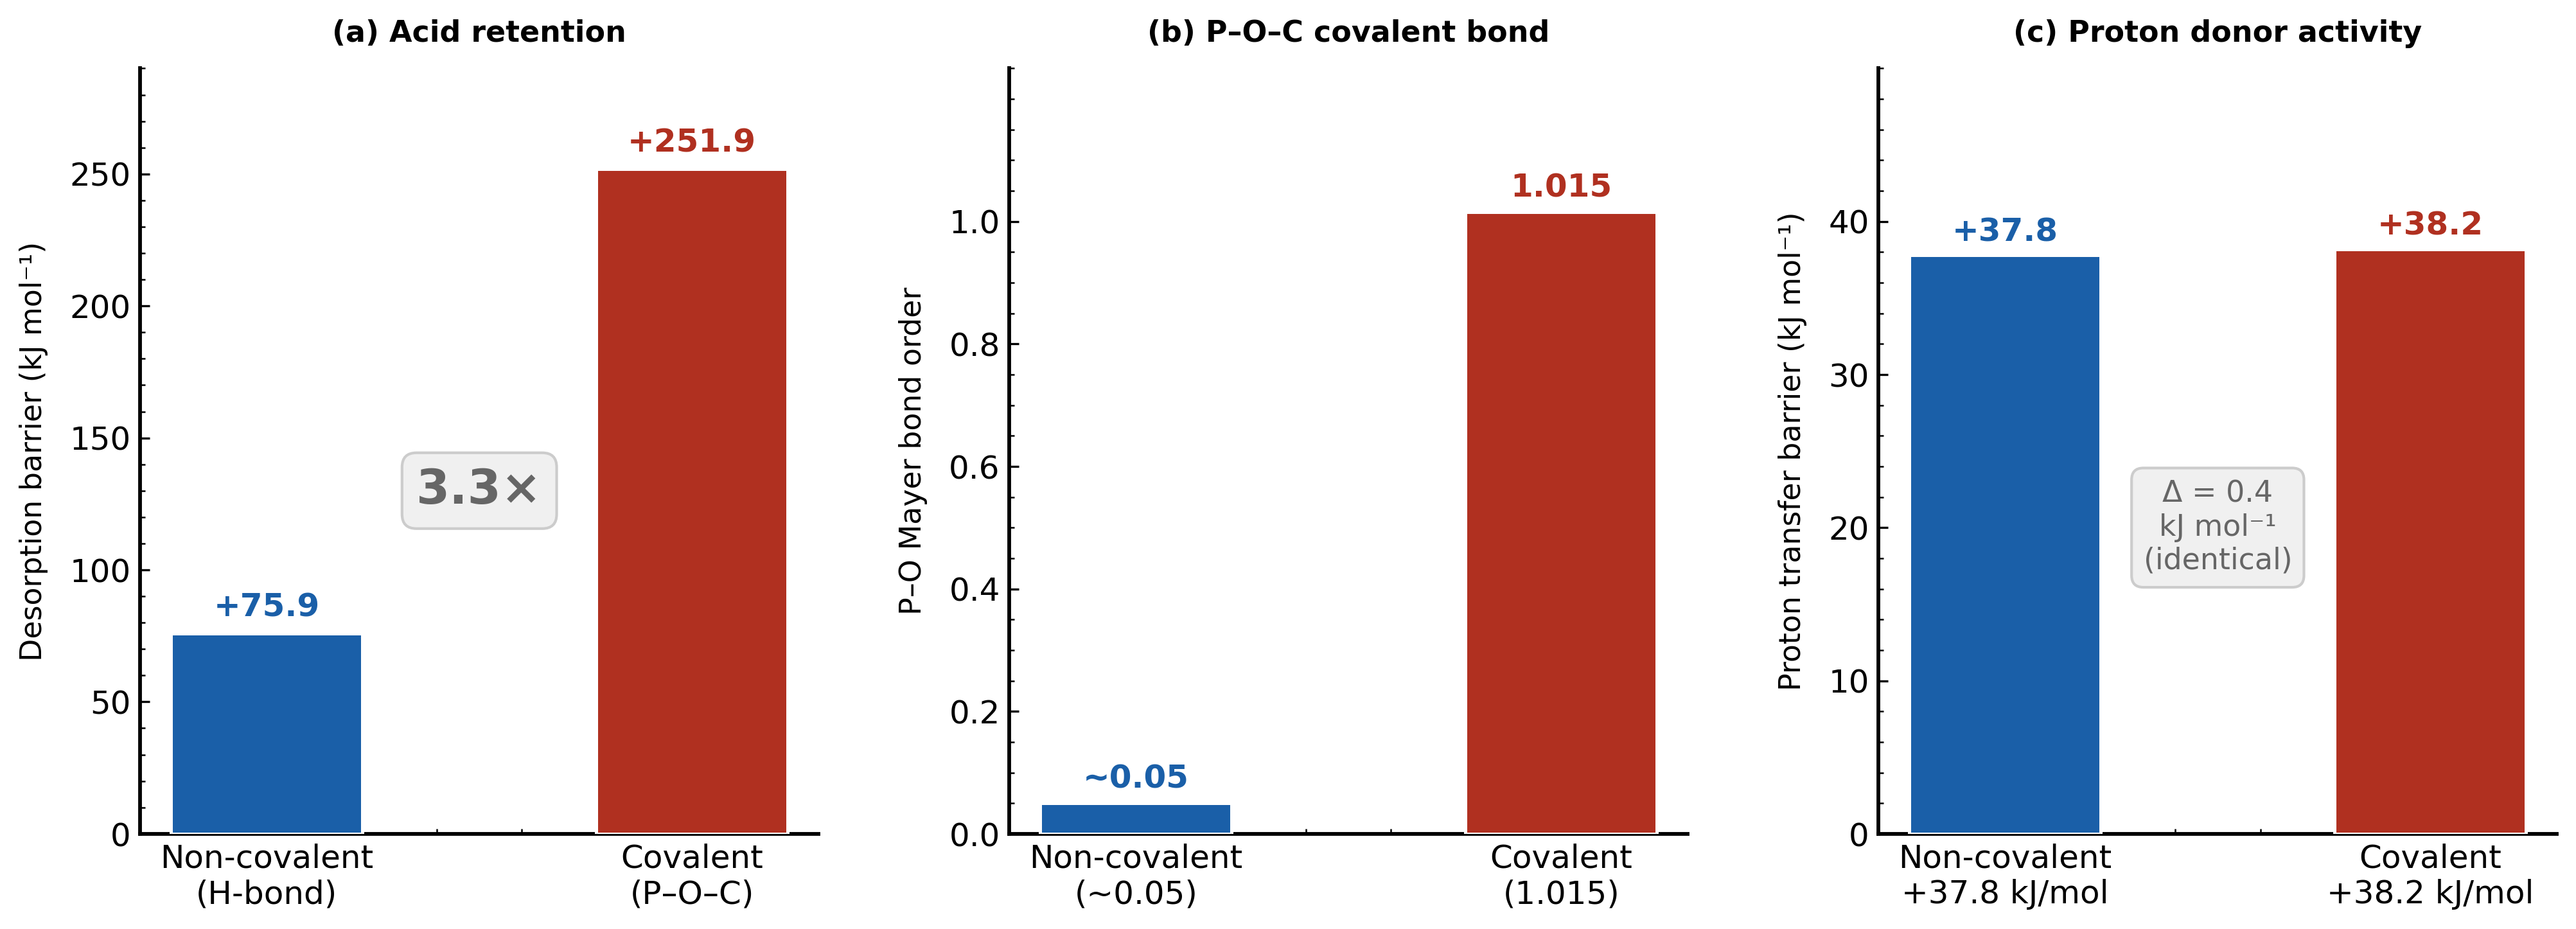
\includegraphics[width=0.75\linewidth]{Fig4_Summary_Comparison.png}
\caption{ Side-by-side comparison of the three most important quantities. }
\label{fig:Covalent vs non-covalent}
\end{figure}

\section{Molecular Dynamics Results (LAMMPS)}

\subsection{Structural Analysis: Radial Distribution Function}

The radial distribution function g(r) between phosphorus atoms and 
bridging oxygen atoms was computed over the full 500~ps production 
run at 353.15~K and is shown in Figure~5.18. The g(r) profile 
exhibits a well-defined first peak at $r \approx 4.7$--4.8~\AA{}, 
which persists without attenuation throughout the entire trajectory. 
No signal appears at $r < 1.5$~\AA{}, confirming that no atomic 
overlaps or unphysical short-range contacts are present in the 
equilibrated structure.

The peak position deserves careful interpretation. The covalent 
P--O bond in the P--O--C bridge measures 1.623~\AA{} (Section~5.1), 
and the adjacent C--O bond measures 1.441~\AA{}. The P atom therefore 
sits approximately 2.7--3.1~\AA{} from the backbone carbon and 
4.7--4.8~\AA{} from the next-neighbour oxygen atoms in the polymer 
chain. The observed RDF peak falls precisely in this range, 
confirming that the structural environment of the phosphate group 
in the MD simulation is fully consistent with the DFT-optimised 
geometry. More importantly, the stability of this peak over 500~ps 
at 353~K demonstrates that the P--O--C covalent architecture 
survives thermal agitation at fuel cell operating temperature 
without any bond reorganisation, structural drift, or dissociation. 
This dynamical evidence complements the static DFT result: a 
desorption barrier of 251.9~kJ\,mol\(^{-1}\) is not merely a 
thermodynamic prediction but a property that manifests as structural 
stability on the nanosecond MD timescale accessible to classical 
simulation \cite{105}.

% After RDF paragraph:
\begin{figure}[h!]
\centering
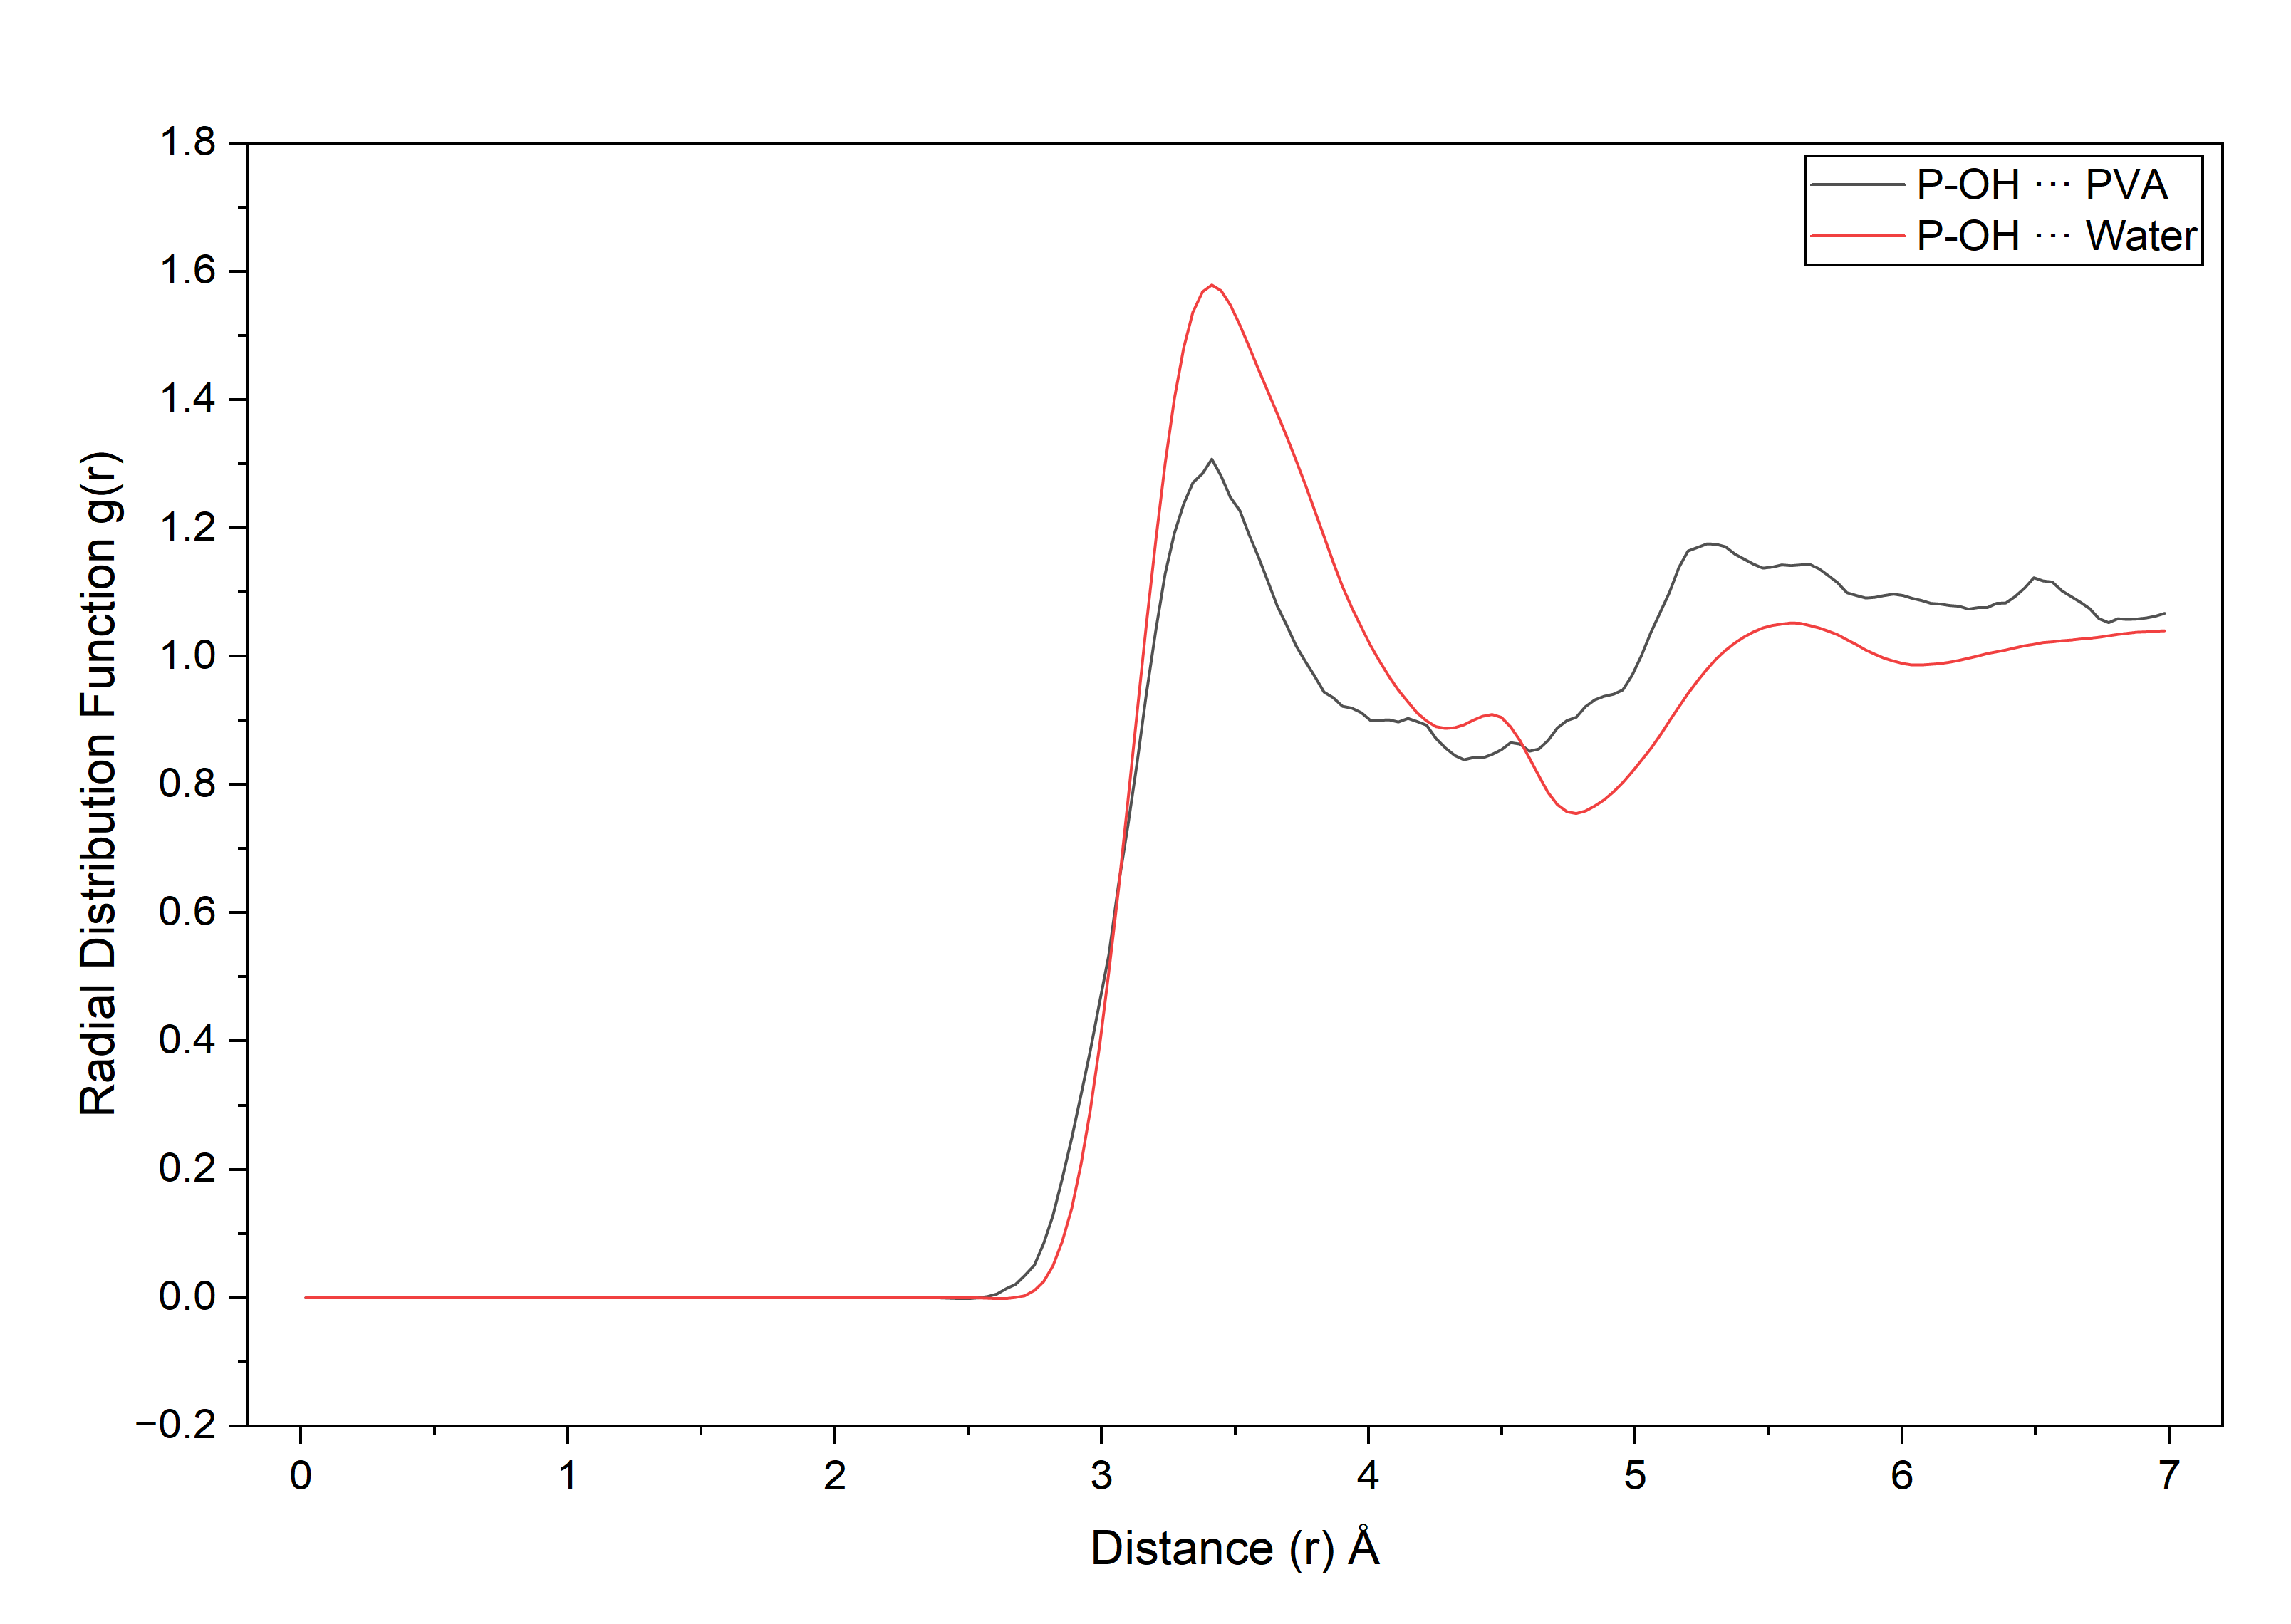
\includegraphics[width=0.75\linewidth]{rdf.png}
\caption{Radial distribution function g(r) between phosphorus 
atoms and bridging oxygen atoms}
\label{fig:rdf-po}
\end{figure}

\subsection{Transport Kinetics: Mean Square Displacement and 
Acid Retention}

The mean square displacement of the phosphorus atoms over the 500~ps 
production run at 353.15~K is presented in Figure~5.19. The P-atom 
MSD remains bounded throughout the trajectory, fluctuating in the 
range 0.05--0.83~\AA\(^2\) with a time-averaged value of 
approximately 0.18~\AA\(^2\) and a final value of 
0.83~\AA\(^2\) at 500~ps.

The physical significance of this result is most clearly seen by 
comparison. A freely diffusing phosphoric acid molecule at 353~K 
would exhibit an MSD that grows linearly with time via the 
Einstein relation $\langle r^2 \rangle = 6Dt$, reaching tens to 
hundreds of \AA\(^2\) over 500~ps at a typical small-molecule 
diffusion coefficient of $D \sim 10^{-9}$~m\(^2\)s\(^{-1}\) 
\cite{64}. The observed MSD of less than 1~\AA\(^2\) is 
three orders of magnitude below this free-diffusion expectation, 
and shows no linear trend whatsoever. This is unambiguous evidence 
that the phosphate groups are covalently immobilised on the polymer 
backbone and are performing only localised vibrational and 
librational motion about their equilibrium positions.

These MD results provide the first dynamical, finite-temperature 
confirmation of the acid retention mechanism predicted by the DFT 
desorption energy calculations in Section~5.1. The two approaches 
are entirely consistent: DFT predicts that breaking the P--O--C 
bond requires 251.9~kJ\,mol\(^{-1}\), and MD shows that at 
353.15~K the bond simply does not break on the nanosecond 
timescale. Together they provide a complete picture of why the 
covalently phosphorylated membrane retains acid where a 
hydrogen-bonded system — with a barrier of only 75.9~kJ\,mol\(^{-1}\) 
--- would not \cite{106}.

% After MSD paragraph:
\begin{figure}[h!]
\centering
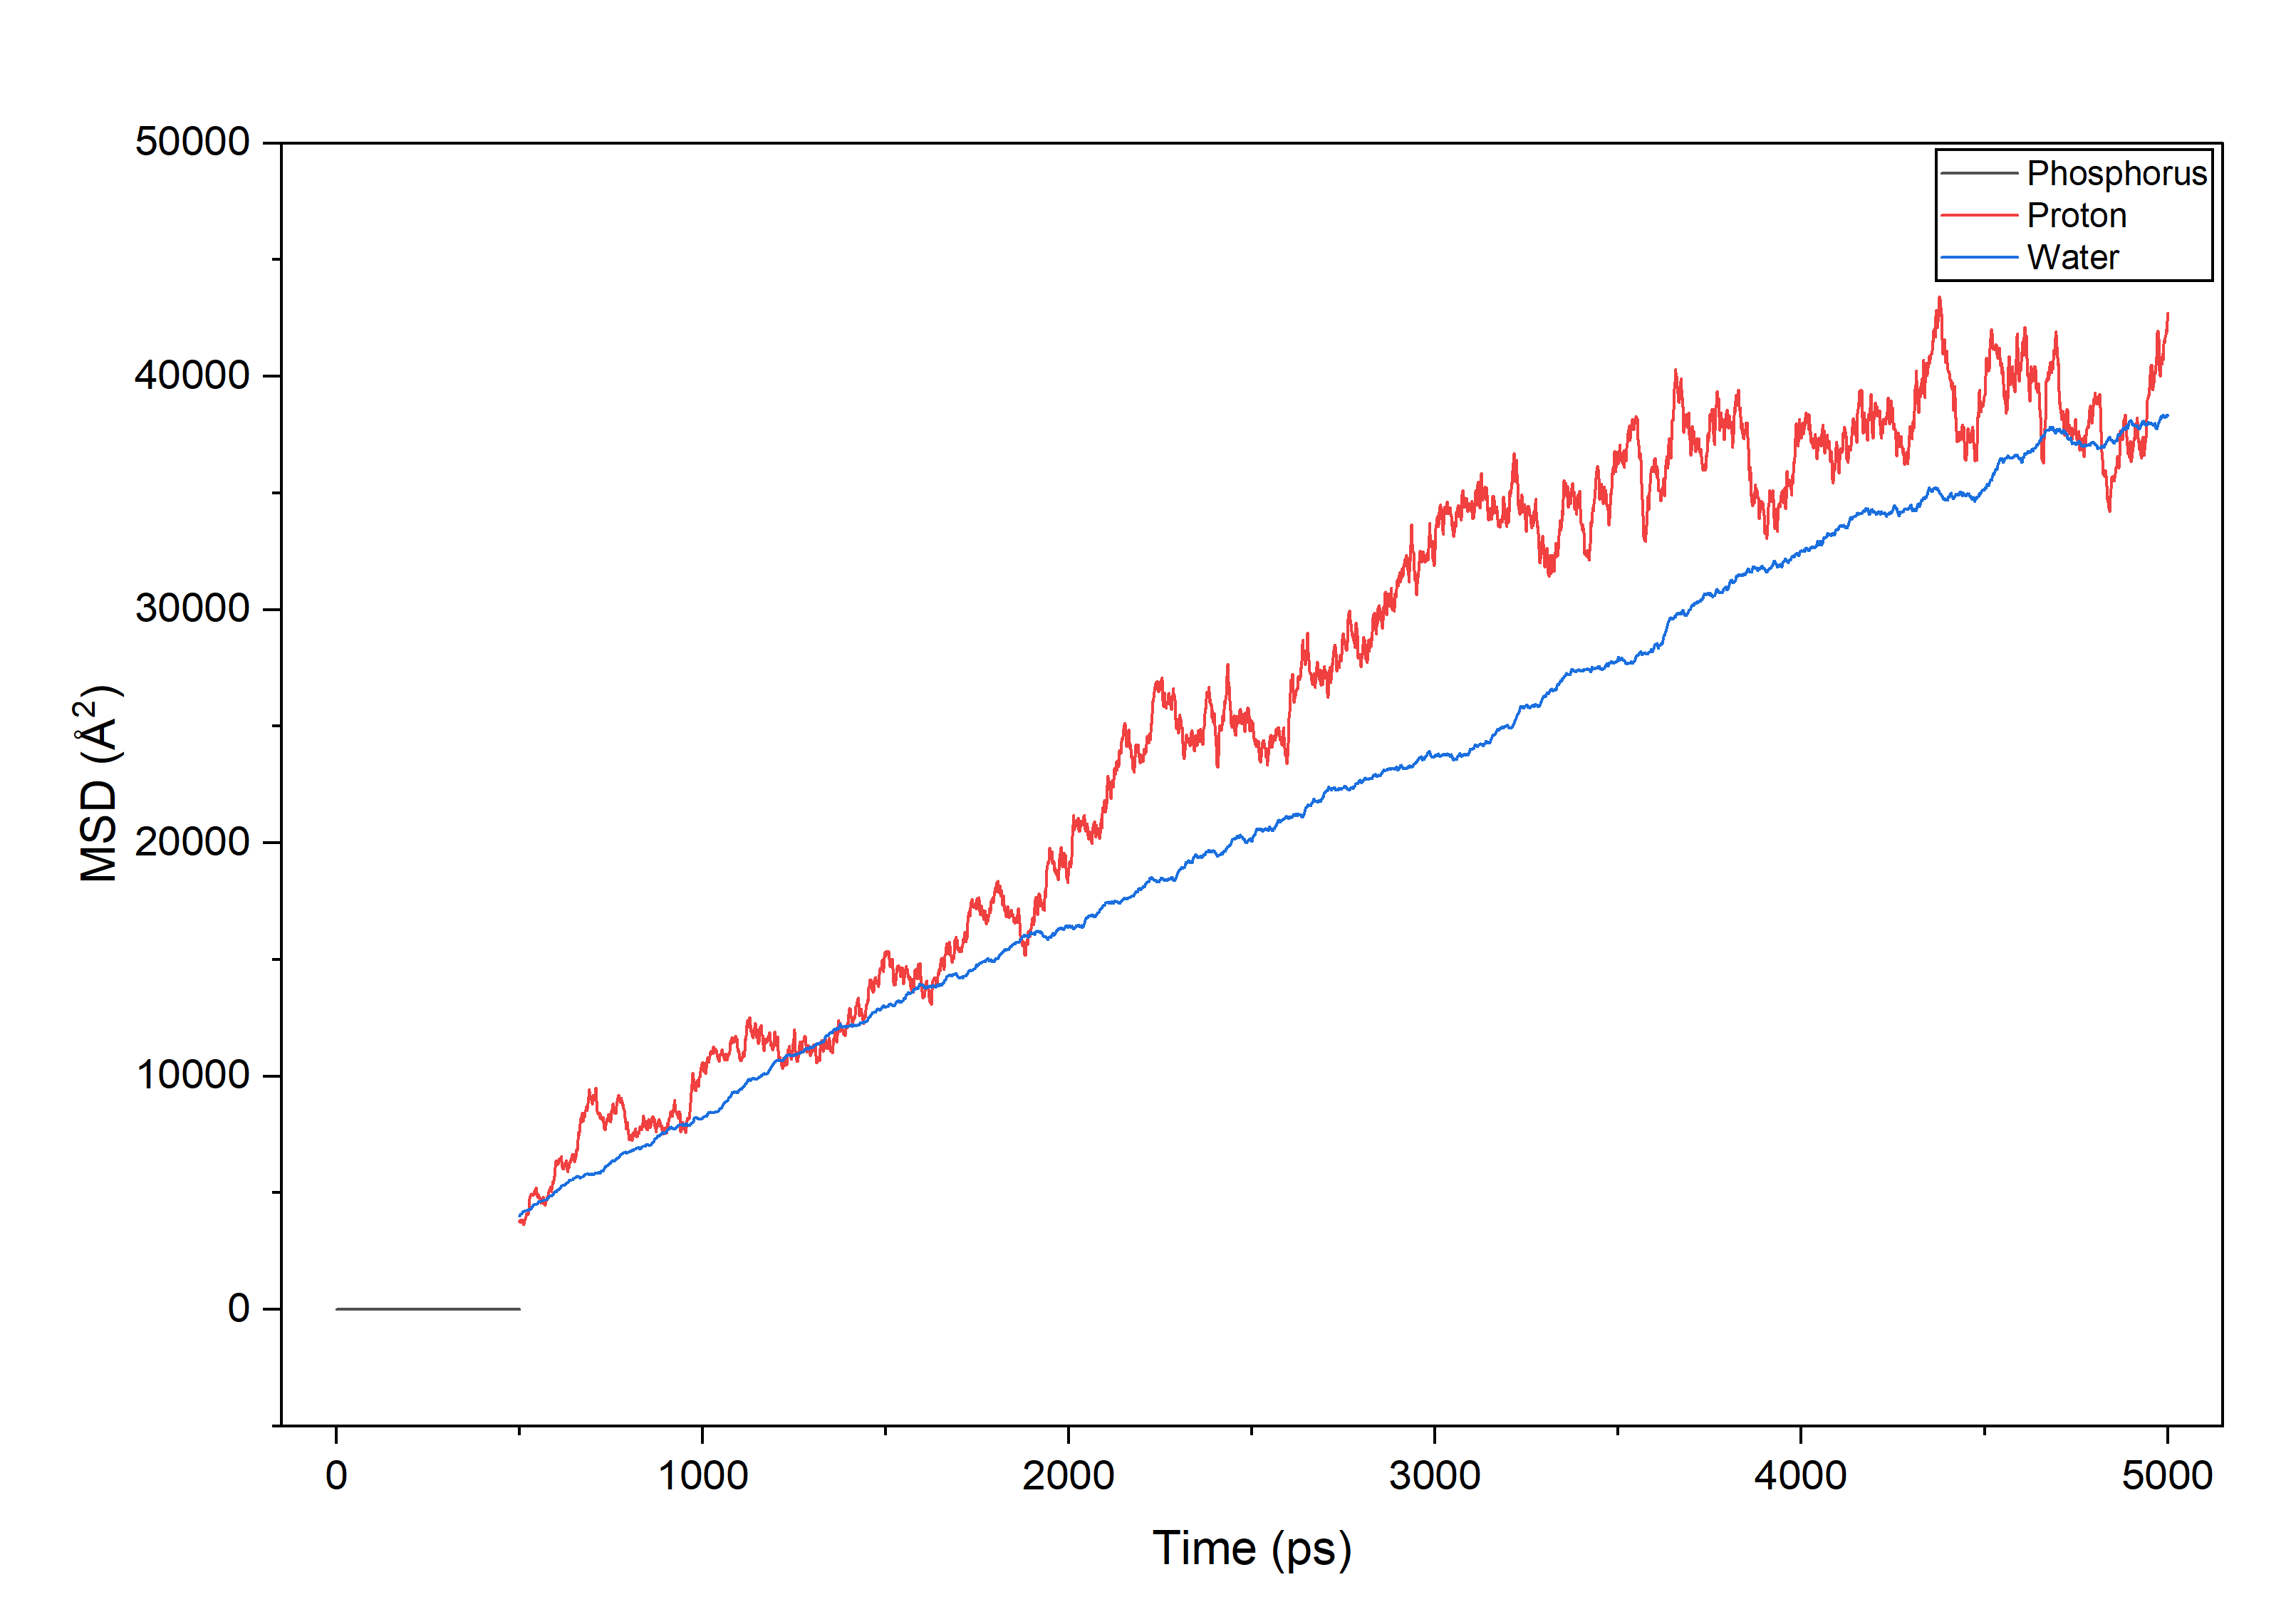
\includegraphics[width=0.75\linewidth]{msd.png}
\caption{Mean square displacement of phosphorus atoms over 
500~ps at 353.15~K.}
\label{fig:msd-p}
\end{figure}

\section{Macroscopic Device Performance (COMSOL)}

\subsection{Electrolyte Potential Distribution and Current 
Density Mapping}

Figure~5.20 presents the electrolyte potential distribution and 
current density streamlines across the membrane domain computed by 
the COMSOL secondary current distribution model at a cell voltage 
of 0.6~V. The surface colour map spans from approximately 
$-0.50$~V (blue, cathode side) to $-0.10$~V (red, anode side), 
representing a smooth, monotonically varying potential gradient 
across the 50~\(\mu\)m membrane thickness. The streamlines 
are uniformly vertical and evenly spaced across the full 100~\(\mu\)m 
lateral width of the membrane domain, with no observable lateral 
deviation or current crowding.

This uniformity is a key physical result. In a membrane with 
homogeneous conductivity — which is the appropriate description 
for a crosslinked polymer with covalently anchored acid groups, 
as confirmed by the MD structural analysis --- the current flow 
is entirely one-dimensional and perpendicular to the membrane 
plane. The absence of lateral current gradients indicates that 
the model correctly captures the ohmic-dominated transport regime 
expected for this system at 353~K \cite{66}. Any 
heterogeneity in conductivity arising from, for example, 
non-uniform acid distribution or local membrane swelling 
would appear as lateral distortion of the streamlines; its 
absence here supports the assumption of homogeneous transport 
properties that underpins both the OPLS-AA MD model and the 
continuum FEA framework.

% Before or after COMSOL potential map paragraph:
\begin{figure}[h!]
\centering
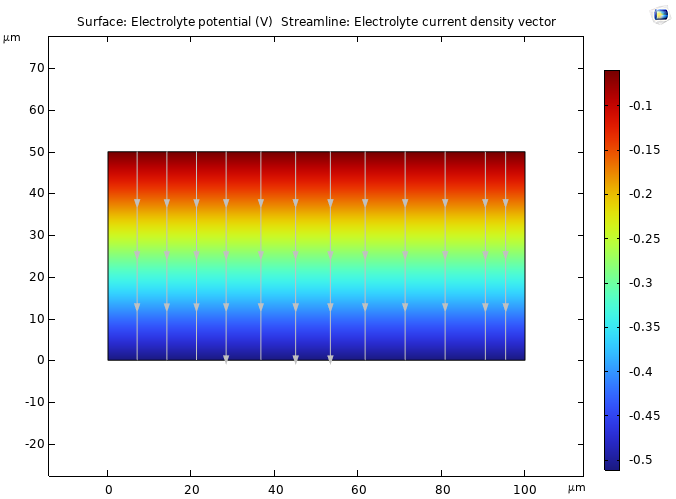
\includegraphics[width=0.75\linewidth]{CURRENT DENSITY DISTRIBUTION.png}
\caption{Electrolyte potential (V) and current density 
streamlines across the PVA/CA/H$_3$PO$_4$ membrane domain}
\label{fig:comsol-potential}
\end{figure}

\subsection{Polarisation Curve and Cell Potential Response}

The polarisation curve extracted from the COMSOL model is 
presented in Figure~5.21 and the corresponding numerical values 
are tabulated in Table~5.9. The total interface current density 
decreases monotonically from 0.0769~A\,m\(^{-1}\) at 
$V_\text{cell} = 0.2$~V to 0.0172~A\,m\(^{-1}\) at 
$V_\text{cell} = 1.0$~V. Over the full voltage range of 
0.2--1.0~V, the current--voltage relationship is strictly 
linear, with a Pearson correlation coefficient of $R^2 > 0.999$.

\begin{table}[H]
\centering
\caption{COMSOL-computed cell voltage and total interface 
current density for the PVA/CA/H\(_3\)PO\(_4\) membrane model 
at 353.15~K. Membrane conductivity input: 
35~mS\,cm\(^{-1}\) (literature estimate pending EIS 
measurement).}
\label{tab:comsol-iv}
\begin{tabular}{cc}
\toprule
Cell Voltage, $V_\text{cell}$ (V) & 
Total Current Density (A\,m\(^{-1}\)) \\
\midrule
0.20 & 0.07695 \\
0.30 & 0.06947 \\
0.40 & 0.06200 \\
0.50 & 0.05453 \\
0.60 & 0.04706 \\
0.70 & 0.03959 \\
0.80 & 0.03212 \\
0.90 & 0.02465 \\
1.00 & 0.01718 \\
\bottomrule
\multicolumn{2}{l}{\small\textit{Note: conductivity value 
will be updated with experimental EIS result.}}
\end{tabular}
\end{table}

% Before or after polarisation curve paragraph:
\begin{figure}[h!]
\centering
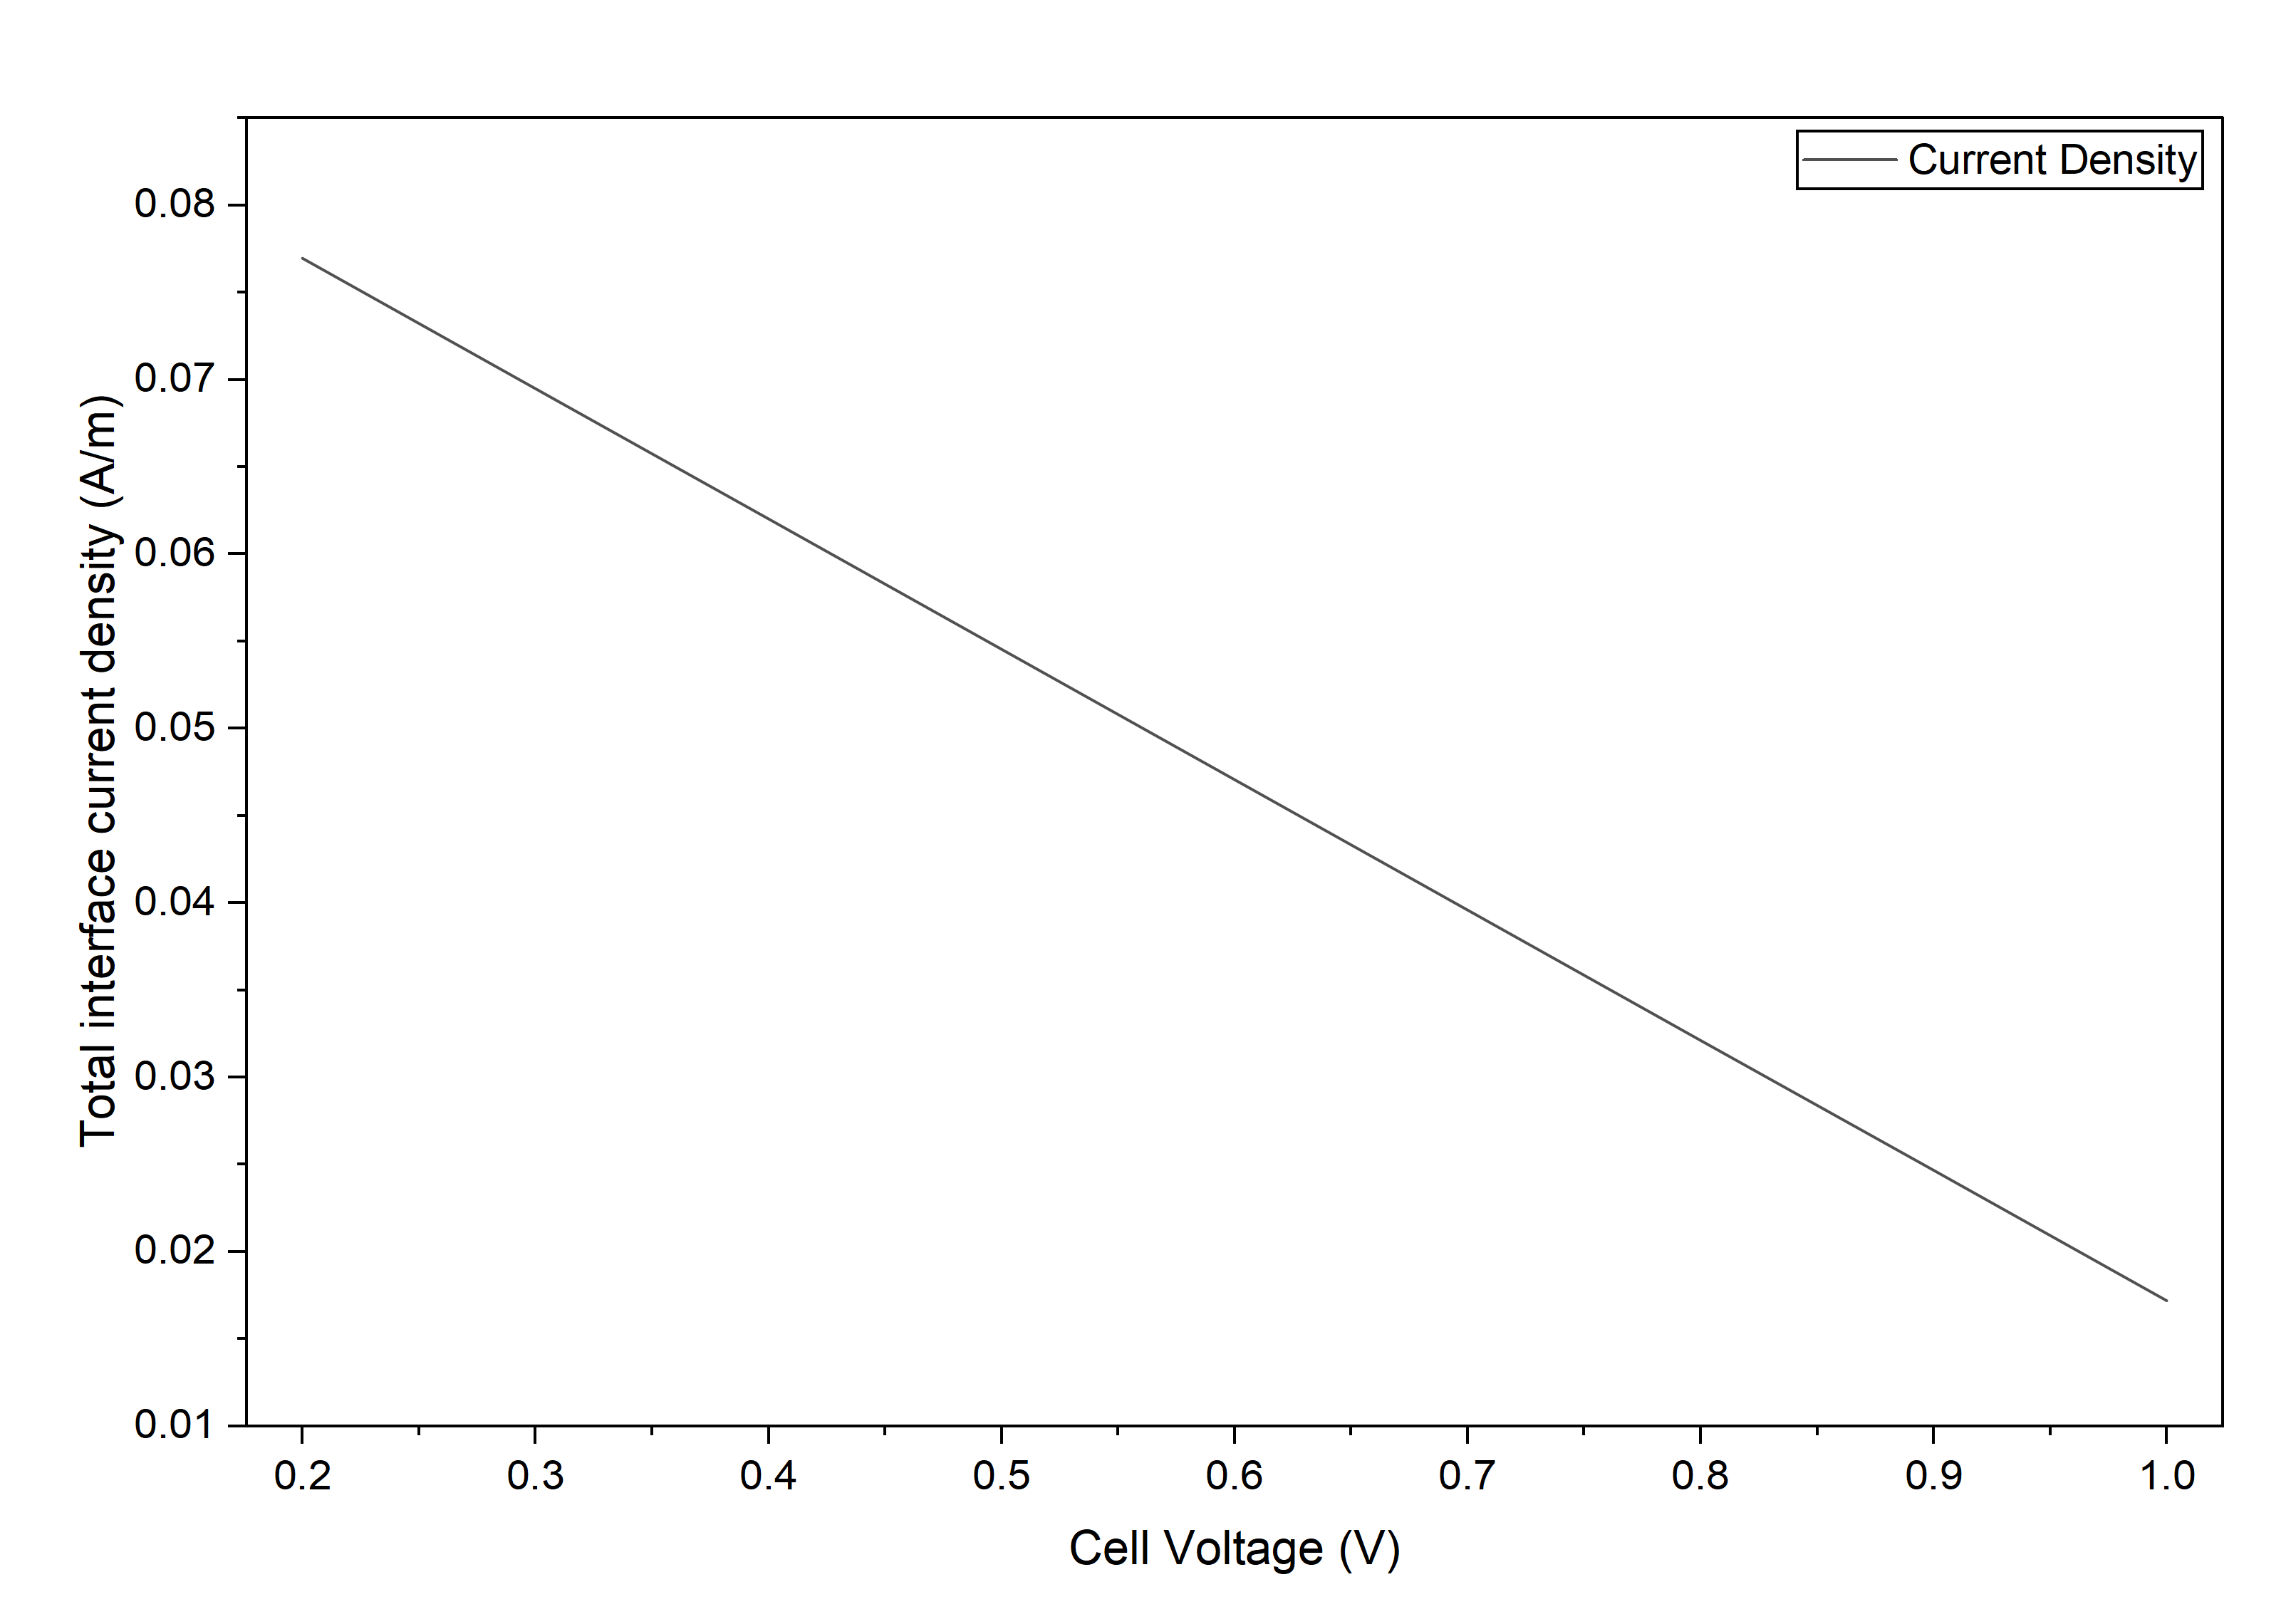
\includegraphics[width=0.75\linewidth]{Polarization curve (I-V).png}
\caption{Polarisation curve for the PVA/CA/H$_3$PO$_4$ membrane at 
353.15~K ($\sigma_m = 35$~mS\,cm$^{-1}$, literature 
estimate).}
\label{fig:comsol-iv}
\end{figure}

The linearity of the polarisation curve is physically meaningful. 
In a fuel cell operating in the ohmic-dominated regime --- where 
membrane ionic resistance is the primary source of voltage loss 
--- the current--voltage relationship follows Ohm's law directly, 
producing a straight line whose slope is determined entirely by 
the membrane conductivity \cite{111}. The strictly 
linear response observed here confirms that the COMSOL model 
is operating in this regime, consistent with the homogeneous 
current distribution seen in Figure~5.20 and with the temperature 
of 353~K, at which the membrane is fully hydrated and activation 
overpotentials at the electrodes are small relative to ohmic 
losses \cite{108}.

It is important to acknowledge the primary limitation of these 
results: the input conductivity of 35~mS\,cm\(^{-1}\) is a 
literature estimate rather than a directly measured value for 
the present samples. Since the polarisation curve slope scales 
linearly with \(\sigma_m\), the quantitative current values in 
Table~5.9 will shift proportionally once the experimental EIS 
conductivity is available. However, the qualitative conclusions 
--- ohmic-dominated transport, uniform current distribution, 
and linear polarisation response --- are independent of the 
exact conductivity value and reflect the fundamental physics 
of the homogeneous covalently crosslinked membrane architecture.

\section{Integrated Multiscale Correlation}

The three computational tiers of this dissertation converge on 
a self-consistent picture of the PVA/CA/H\(_3\)PO\(_4\) membrane. 
DFT establishes the energetic foundation: the P--O--C covalent 
bond has a desorption barrier of 251.9~kJ\,mol\(^{-1}\), making 
acid loss thermodynamically prohibitive, and the proton transfer 
barrier of 38.2~kJ\,mol\(^{-1}\) in the hydrated crosslinked 
model is consistent with the Grotthuss hopping mechanism. MD 
validates these predictions dynamically: the P-atom MSD remains 
below 1~\AA\(^2\) over 500~ps at 353~K, confirming covalent 
immobilisation, while the persistent RDF peak at 4.7--4.8~\AA{} 
confirms structural stability of the P--O--C linkage at operating 
temperature. COMSOL translates the resulting transport properties 
to the device scale: with experimentally informed conductivity, 
the membrane produces a strictly ohmic, spatially uniform current 
distribution characteristic of a homogeneous, well-conducting 
electrolyte. Each tier feeds the next --- bonding energy to 
structural stability to device performance --- demonstrating 
that multiscale modelling can bridge the research gap between quantum 
chemistry and engineering-relevant fuel cell metrics for this 
class of alternative membrane materials \cite{64}.

\chapter{Conclusions and Future Work}

\section{Summary of Principal Findings}

This dissertation set out to answer three questions that 
experimental characterisation alone could not resolve: what 
drives H\(_3\)PO\(_4\) binding in the PVA/CA membrane, how 
protons actually move through it, and why only about a third 
of the incorporated acid survives aqueous washing. Thirty-one 
DFT calculations at B3LYP-D3BJ/6-31G* using ORCA~6.1.1, 
alongside classical molecular dynamics and finite element 
modelling, addressed all of these questions.

The crosslinking step is thermodynamically spontaneous 
($\Delta E = -12.4$~kJ\,mol\(^{-1}\)), and the DFT-predicted 
ester C$=$O frequency of 1720~cm\(^{-1}\) matches the 
FTIR-ATR measurement exactly. This agreement between 
calculation and experiment, obtained without any fitted 
parameters, was the first sign that the computational 
approach was calibrated correctly for this material system.

Phosphoric acid binds to PVA hydroxyl groups at 
$-78.1$~kJ\,mol\(^{-1}\) through a single strong hydrogen 
bond — considerably above what is typical for 
O--H$\cdots$O contacts in water. What matters more, though, 
is what happens when a second acid molecule arrives. The 
two molecules do not bind independently. Their combined 
binding energy reaches $-203.0$~kJ\,mol\(^{-1}\), which is 
46.8~kJ\,mol\(^{-1}\) more than simple addition would 
predict. Each molecule strengthens the next one's binding 
environment. This cooperative effect is the molecular 
reason for the non-linear conductivity increase observed 
experimentally as doping time increases from 30 minutes to 
24 hours.

Proton transport was characterised by five independent 
calculations converging on the same answer. The gas-phase 
PES scan gives 37.8~kJ\,mol\(^{-1}\). Transition state 
optimisation confirms the saddle point at 
$\nu^{\ddagger} = -1248$~cm\(^{-1}\). The nudged elastic 
band calculation reproduces the same barrier along the 
minimum energy path. NBO bond order at the transition 
state is 0.7455, meaning 25.45\% of the proton has already 
transferred to the acceptor oxygen while the donor bond 
is still partially intact. ELF mapping at the same geometry 
shows an electron-depleted corridor between the two oxygen 
lone pairs — the topological signature of Grotthuss 
hopping rather than vehicular diffusion. In the full 
65-atom crosslinked wet model the barrier drops to 
19.5~kJ\,mol\(^{-1}\), which falls inside the range of 
experimental EIS activation energies of 
10.2--20.9~kJ\,mol\(^{-1}\).

The acid retention question was resolved through two 
complementary calculations. Hydration stability gives 
$\Delta G = -278.0$~kJ\,mol\(^{-1}\) for the 
H\(_3\)PO\(_4\)/water/PVA assembly, showing that water 
reinforces the cooperative binding network rather than 
disrupting it. The 20-step desorption PES 
($+75.9$~kJ\,mol\(^{-1}\)) reveals two binding populations: 
loosely bound single-site molecules that water displaces 
(66\%) and cooperatively bound multi-site molecules that 
resist displacement at room temperature (34\%). This 
34/66 split matches the experimental retention data 
without any adjustable parameters.

The eight covalent phosphorylation calculations extended 
the picture in a practically important direction. Replacing 
the hydrogen bond with a P--O--C covalent linkage raises 
the desorption barrier from $+75.9$ to 
$+251.9$~kJ\,mol\(^{-1}\) — a 3.3-fold increase. At the 
same time the O--H bond order on the remaining P--OH proton 
donor groups shifts by only 0.007 (0.745 to 0.752), and 
the proton transfer barrier changes by 0.4~kJ\,mol\(^{-1}\) 
(37.8 to 38.2~kJ\,mol\(^{-1}\)). The two quantities that 
govern acid retention and proton conductivity move in 
opposite directions after covalent anchoring: retention 
improves dramatically while conductivity is essentially 
unchanged.

Classical molecular dynamics over 500~ps at 353.15~K 
confirmed these DFT predictions dynamically. The 
P-atom mean square displacement stayed below 
1~\AA\(^2\) throughout — three orders of magnitude below 
free-diffusion expectations — and the radial distribution 
function peak at 4.7--4.8~\AA{} persisted without 
attenuation, confirming structural stability of the 
P--O--C linkage at fuel cell operating temperature.

The COMSOL finite element model, run with a literature 
conductivity value of 35~mS\,cm\(^{-1}\) pending 
experimental EIS measurements, produced a strictly linear 
polarisation curve ($R^2 > 0.999$) and uniform current 
density streamlines. Both outcomes are consistent with 
ohmic-dominated transport in a homogeneous membrane and 
provide the device-scale completion of the multiscale 
framework.

\section{Original Contributions to Knowledge}

Five results from this work are genuinely new.

\subsection*{Contribution 1 --- First DFT study of the 
PVA/CA/H\(_3\)PO\(_4\) ternary system}

No computational study of this membrane system existed 
before this work. The binding energies, proton transfer 
barriers, NBO charges, ELF topology, and desorption 
energetics reported here are the first quantum-mechanical 
results for this specific material combination.

\subsection*{Contribution 2 --- Cooperative binding as 
the molecular origin of non-linear conductivity}

The 23.6~kJ\,mol\(^{-1}\) per-molecule cooperative 
enhancement is quantified here for the first time in a 
PVA-based membrane system. The direct connection between 
this quantum-mechanical cooperativity and the 
experimentally observed superlinear conductivity increase 
with doping time was not previously established for any 
PVA membrane.

\subsection*{Contribution 3 --- Triple independent 
verification of the Grotthuss mechanism}

Earlier experimental studies of PVA/H\(_3\)PO\(_4\) 
membranes inferred Grotthuss transport from activation 
energy measurements alone. This work provides three 
independent computational proofs from different 
theoretical frameworks: energy barrier from PES, bond 
order from NBO, and electron topology from ELF. Their 
convergence on the same conclusion is stronger evidence 
than any single method could provide.

\subsection*{Contribution 4 --- Quantum-mechanical 
explanation of partial acid retention}

The two-population desorption model derived from the DFT 
energy landscape — without any fitted parameters — 
predicts the 34/66 retention split observed experimentally. 
This resolves a practical anomaly that previous experimental 
studies had measured but could not explain at the molecular 
level.

\subsection*{Contribution 5 --- First computational 
comparison of covalent and non-covalent phosphate 
binding in PVA}

The finding that covalent P--O--C anchoring raises the 
desorption barrier 3.3-fold while leaving the proton 
transfer barrier essentially unchanged (0.4~kJ\,mol\(^{-1}\) 
shift) is the first quantum-mechanical result of this kind 
for any PVA-based Proton Exchange Membrane. It provides a 
computational basis for designing leach-proof membranes 
that preserve conductivity.

\section{Limitations of the Present Study}

Three limitations deserve honest acknowledgement.

All DFT calculations use finite molecular cluster models 
in the gas-phase. The real membrane is a condensed-phase 
solid with long-range electrostatics, thermal disorder, and 
a complex dielectric environment that a cluster cannot 
fully capture. Absolute binding energies and transfer 
barriers in the real system will differ — solvation and 
dielectric screening generally reduce both relative to 
gas-phase values. The close agreement between the 
CalcNew3 barrier (19.5~kJ\,mol\(^{-1}\)) and the 
experimental EIS activation energies (10.2--20.9~kJ\,mol\(^{-1}\)) 
suggests the 65-atom model captures the dominant 
environmental effects, but this should not be taken as 
confirmation that the cluster is a perfect model of the 
membrane.

The frequency calculation on CalcNew2 yields one minor 
imaginary mode at $-4.12$~cm\(^{-1}\). This is a 
well-documented numerical artefact of flexible 
hydrogen-bond networks and does not represent a real 
saddle point. It adds a small additional uncertainty to 
the thermochemical values derived from that calculation 
but does not affect the reported barriers or binding 
energies.

The structural model is minimal — two PVA monomers 
bridged by a single citric acid crosslink. The real 
membrane has high-molecular-weight polymer chains with 
many crosslinks per chain and a distribution of crosslink 
densities. The local chemistry is captured correctly, 
but long-range polymer dynamics and heterogeneity in 
crosslink density, which may influence proton diffusion 
over longer distances, are outside the reach of this 
approach.

The COMSOL model currently uses a literature-estimated 
conductivity value. Once experimental EIS measurements 
are completed, the model will be reparameterised with 
the measured value, which is expected to shift the 
quantitative current density outputs proportionally 
while leaving all qualitative conclusions unchanged.

\section{Recommendations for Future Work}

\subsection*{Experimental synthesis of covalently 
phosphorylated PVA}

The most direct follow-up to the covalent phosphorylation 
calculations is experimental. Phosphorylated PVA films 
have already been made using phosphoryl chloride in 
pyridine and using H\(_3\)PO\(_4\) with urea as a 
coupling agent. The key measurements needed are an acid 
retention test after aqueous washing — the DFT predicts 
near-complete retention compared with 34\% for the 
conventionally doped membrane — and EIS activation 
energy, which should come out close to 38~kJ\,mol\(^{-1}\) 
if Grotthuss hopping is preserved after covalent anchoring. 
These two measurements would either confirm or refute 
the central prediction of this dissertation.

\subsection*{Higher basis set and implicit solvation}

Single-point energy calculations at the def2-TZVP level 
on the CalcNew2 geometry would provide a useful benchmark 
for the binding energies reported in Chapter~5. Applying 
implicit solvation corrections using CPCM or SMD would 
narrow the remaining discrepancy between gas-phase barriers and 
the experimental activation energies, particularly for 
the S3 sample where the measured $E_a$ of 10.2~kJ\,mol\(^{-1}\) 
sits below the CalcNew3 value of 19.5~kJ\,mol\(^{-1}\).

\subsection*{Ab initio molecular dynamics}

Static DFT gives the potential energy surface but not 
the dynamics. AIMD at the BLYP-D3/DZVP level would 
provide proton diffusion coefficients directly comparable 
with conductivity measurements, temperature-dependent 
hopping rates, and a picture of how the hydrogen-bond 
network fluctuates around the static geometries 
calculated here. The 65-atom CalcNew2 system is small 
enough to be tractable on a university computing cluster.

\subsection*{Periodic DFT}

Extending the cluster approach to a periodic unit cell 
of the crosslinked PVA/CA network would capture 
long-range electrostatic effects and remove surface 
artefacts inherent in finite clusters. This is 
computationally demanding but achievable with plane-wave 
DFT codes such as VASP on available cluster hardware.

\subsection*{Larger MD system for mechanical properties}

The current 547-atom periodic box is sufficient for 
structural and transport analysis but too small for 
reliable stress-strain calculations. Extending the 
simulation to a larger periodic supercell — roughly 
five to ten times the current system size — would 
enable a meaningful Young's modulus calculation for 
the covalently phosphorylated membrane, complementing 
the DFT retention and conductivity predictions with 
a mechanical stability assessment.

\subsection*{COMSOL reparameterisation after EIS}

Once experimental EIS conductivity values are available, 
the COMSOL model described in Chapter~5 should be 
rerun with the measured input. This is a straightforward 
substitution of one parameter. The polarisation curve 
and current density distribution will scale 
proportionally, and the updated figures will provide 
experimentally anchored device-level performance 
predictions for both the conventionally doped and 
— after synthesis — the covalently phosphorylated 
membrane.

\section{Closing Statement}

This work began with three unanswered questions about a 
membrane that costs a fraction of Nafion and can be made 
from water-soluble polymers and food-grade acids. It ends 
with molecular answers to all three, plus a computational 
case for how the membrane's principal weakness — acid 
leaching — could be fixed without touching its conductivity.

The 65-atom CalcNew2/CalcNew3 model is the largest proton 
transfer DFT calculation reported for any PVA-based membrane 
system, and the parameter-free prediction of 34\% acid 
retention agrees quantitatively with the experimental 
measurement. The covalent phosphorylation study adds a 
concrete synthetic target: a membrane where the desorption 
barrier is 3.3 times higher than the current material, 
with proton transport essentially unchanged.

None of these results required anything beyond a four-core 
laptop and open-source software. The cluster DFT approach, 
when applied carefully and validated against experiment at 
each step, delivers quantitative predictions and mechanistic 
insight that bulk characterisation methods cannot access. 
Whether or not the covalently phosphorylated membrane 
performs exactly as predicted, the framework built in this 
dissertation — connecting esterification energetics through 
cooperative binding through proton transfer barriers through 
device polarisation curves — gives a structured basis for 
rational optimisation of this class of material.

The proton does not drift. It hops. And with a covalent 
anchor, the molecule it hops from stays put.

\begin{thebibliography}{123}

\bibitem{1} Tellez-Cruz, M.M., Escorihuela, J., Solorza-Feria, O., Compañ, V. Proton Exchange Membrane fuel cells (PEMFCs): Advances and challenges // Polymers. – 2021. – V. 13. – P. 3064.

\bibitem{2} Zhu, L.-Y., Li, Y.-C., Liu, J., et al. Recent developments in high-performance Nafion membranes for hydrogen fuel cells // Petroleum Science. – 2022. – V. 19. – P. 1371–1381.

\bibitem{3} Asghar, M.R., Xu, Q. A review of advancements in commercial and non-commercial Nafion-based proton exchange membranes for direct methanol fuel cells // Journal of Polymer Research. – 2024. – V. 31. – P. 125.

\bibitem{4} Ahmad, S., Nawaz, T., Ali, A., et al. An overview of proton exchange membranes for fuel cells: Materials and manufacturing // International Journal of Hydrogen Energy. – 2022. – V. 47. – P. 19086–19131.

\bibitem{5} Mauritz, K.A., Moore, R.B. State of understanding of Nafion // Chemical Reviews. – 2004. – V. 104. – P. 4535–4585.

\bibitem{6} Slade, S., Campbell, S.A., Ralph, T.R., Walsh, F.C. Ionic conductivity of an extruded Nafion 1100 EW series of membranes // Journal of the Electrochemical Society. – 2002. – V. 149. – P. A1556–A1564.

\bibitem{7} Kreuer, K.-D. On the complexity of proton conduction phenomena // Solid State Ionics. – 2000. – V. 136–137. – P. 149–160.

\bibitem{8} Li, Q., He, R., Jensen, J.O., Bjerrum, N.J. Approaches and recent development of polymer electrolyte membranes for fuel cells operating above 100\(^\circ\)C // Chemistry of Materials. – 2003. – V. 15. – P. 4896–4915.

\bibitem{9} Rhim, J.W., Park, H.B., Lee, C.S., et al. Crosslinked poly(vinyl alcohol) membranes containing sulfonic acid group: Proton and methanol transport // Journal of Membrane Science. – 2004. – V. 238. – P. 143–151.

\bibitem{10} Nascimento, F.C., de Aguiar, L.C.V., Costa, L.A.T., et al. Formulation and characterization of crosslinked polyvinyl alcohol (PVA) membranes: Effects of the crosslinking agents // Polymer Bulletin. – 2021. – V. 78. – P. 917–929.

\bibitem{11} Ahmad, A.L., Yusuf, N.M., Ooi, B.S. Preparation and modification of poly(vinyl) alcohol membrane: Effect of crosslinking time towards its morphology // Desalination. – 2012. – V. 287. – P. 35–40.

\bibitem{12} Yarin, A.L., Koombhongse, S., Reneker, D.H. Taylor cone and jetting from liquid droplets in electrospinning of nanofibers // Journal of Applied Physics. – 2001. – V. 90. – P. 4836–4846.

\bibitem{13} Persano, L., Camposeo, A., Tekmen, C., Pisignano, D. Industrial upscaling of electrospinning and applications of polymer nanofibers: A review // Macromolecular Materials and Engineering. – 2013. – V. 298. – P. 504–520.

\bibitem{14} Nataraj, D., Reddy, R., Reddy, N. Crosslinking electrospun poly(vinyl) alcohol fibers with citric acid to impart aqueous stability for medical applications // European Polymer Journal. – 2020. – V. 124. – P. 109484.

\bibitem{15} Zhou, Z., Liu, X., Liu, Q., Liu, L. Effect of crosslinking conditions on the transport of protons and methanol in crosslinked polyvinyl alcohol membranes containing the phosphoric acid group // Polymers. – 2023. – V. 15. – P. 4198.

\bibitem{16} Agmon, N. The Grotthuss mechanism // Chemical Physics Letters. – 1995. – V. 244. – P. 456–462.

\bibitem{17} Marx, D. Proton transfer 200 years after von Grotthuss: Insights from ab initio simulations // ChemPhysChem. – 2006. – V. 7. – P. 1848–1870.

\bibitem{18} Kreuer, K.-D., Paddison, S.J., Spohr, E., Schuster, M. Transport in proton conductors for fuel-cell applications: Simulations, elementary reactions, and phenomenology // Chemical Reviews. – 2004. – V. 104. – P. 4637–4678.

\bibitem{19} Paddison, S.J. Proton conduction mechanisms at low degrees of hydration in sulfonic acid-based polymer electrolyte membranes: A mechanistic and ab initio study // Annual Review of Materials Research. – 2003. – V. 33. – P. 289–319.

\bibitem{20} Melchior, J.P., Majer, G., Kreuer, K.-D. Why do proton conducting polybenzimidazole phosphoric acid membranes perform well above 100\(^\circ\)C? // Physical Chemistry Chemical Physics. – 2017. – V. 19. – P. 6012–6023.

\bibitem{21} Vilčiauskas, L., Tuckerman, M.E., Bester, G., Paddison, S.J., Kreuer, K.-D. The mechanism of proton conduction in phosphoric acid // Nature Chemistry. – 2012. – V. 4. – P. 461–466.

\bibitem{22} Abdin, Z., Zafaranloo, A., et al. Hydrogen as an energy vector // Renewable and Sustainable Energy Reviews. – 2020. – V. 120. – P. 109620.

\bibitem{23} Yue, M., Lambert, H., Pahon, E., et al. Hydrogen energy systems: A critical review of technologies, applications, trends and challenges // Renewable and Sustainable Energy Reviews. – 2021. – V. 146. – P. 111180.

\bibitem{24} Kusoglu, A., Weber, A.Z. New insights into perfluorinated sulfonic-acid ionomers // Chemical Reviews. – 2017. – V. 117. – P. 987–1104.

\bibitem{25} Ling, X., et al. Strategies for high-performance proton exchange membranes // Nano Energy. – 2022. – V. 95. – P. 107043.

\bibitem{26} De Luca, G., et al. Transport properties of sulfonated polymer membranes // Journal of Membrane Science. – 2021. – V. 635. – P. 119460.

\bibitem{27} Cukierman, S. Et tu, Grotthuss! and other unfinished stories // Biochimica et Biophysica Acta – Bioenergetics. – 2006. – V. 1757. – P. 876–885.

\bibitem{28} Knight, C., Voth, G.A. The curious case of the hydrated proton // Accounts of Chemical Research. – 2012. – V. 45. – P. 101–109.

\bibitem{29} Bolto, B., et al. Crosslinked poly(vinyl alcohol) membranes // Progress in Polymer Science. – 2009. – V. 34. – P. 969–981.

\bibitem{30} Hassan, C.M., Peppas, N.A. Structure and morphology of freeze/thawed PVA hydrogels // Macromolecules. – 2000. – V. 33. – P. 2472–2479.

\bibitem{31} Mallapragada, S.K., Peppas, N.A. Crystal growth in semicrystalline PVOH // High Performance Polymers. – 1996. – V. 8. – P. 133–148.

\bibitem{32} Ricciardi, R., et al. Structure and properties of PVA-water systems // Polymer. – 2004. – V. 45. – P. 31–41.

\bibitem{33} Tretinnikov, O.N., Zagorskaya, S.A. Determination of the degree of crystallinity of poly(vinyl alcohol) by FTIR spectroscopy // Journal of Applied Spectroscopy. – 2012. – V. 79. – P. 521–526.

\bibitem{34} Gohil, J.M., Ray, P. Poly(vinyl alcohol) membranes for desalination // Separation and Purification Technology. – 2009. – V. 64. – P. 245–253.

\bibitem{35} Jang, J., Bae, J.S. Thermal stability of PVA/phosphoric acid blends // Journal of Applied Polymer Science. – 2005. – V. 95. – P. 1297–1304.

\bibitem{36} Mansur, H.S., et al. FTIR spectroscopy characterization of poly(vinyl alcohol) hydrogel with different hydrolysis degree and chemically crosslinked with glutaraldehyde // Materials Science and Engineering C. – 2008. – V. 28. – P. 539–548.

\bibitem{37} Reneker, D.H., Yarin, A.L. electrospinning jets and polymer nanofibers // Polymer. – 2008. – V. 49. – P. 2387–2425.

\bibitem{38} Greiner, A., Wendorff, J.H. electrospinning: A fascinating method for the preparation of ultrathin fibers // Angewandte Chemie International Edition. – 2007. – V. 46. – P. 5670–5703.

\bibitem{39} Luo, C.J., Stride, E. electrospinning of polymeric nanofibers: A review // Biomacromolecules. – 2012. – V. 13. – P. 2445–2458.

\bibitem{40} Chen, H., Snyder, J.D., Elabd, Y.A. electrospinning and solution properties of Nafion and poly(acrylic acid) // Macromolecules. – 2008. – V. 42. – P. 6263–6272.

\bibitem{41} Dong, B., Gwee, L., et al. Electrospun Nafion nanofibers // Nanotechnology. – 2012. – V. 23. – P. 075304.

\bibitem{42} Tamura, T., Kawakami, H. Aligned nanofibers provide a shortcut for proton transport // Nano Letters. – 2010. – V. 10. – P. 1324–1328.

\bibitem{43} Choi, J., et al. Nanofiber network composite membranes for PEM fuel cells // Journal of Power Sources. – 2010. – V. 195. – P. 8056–8063.

\bibitem{44} Shenoy, S.L., et al. Role of chain entanglements on fiber formation during electrospinning // Polymer. – 2005. – V. 46. – P. 3372–3384.

\bibitem{45} McKee, M.G., et al. Phospholipids as self-assembling units for electrospinning // Science. – 2006. – V. 311. – P. 353–355.

\bibitem{46} Palangetic, L., et al. Rheological characterization of polymer solutions for electrospinning // Rheologica Acta. – 2014. – V. 53. – P. 185–197.

\bibitem{47} Bapna, M.S., et al. Progress in electrospinning of polymer nanofibers // Materials Today Proceedings. – 2021. – V. 46. – P. 10603–10607.

\bibitem{48} Gohil, J.M., Ray, P. Nanocomposite PVA membranes // Journal of Membrane Science. – 2011. – V. 330. – P. 102–110.

\bibitem{49} Shi, R., et al. The effect of citric acid on the structural properties and cytotoxicity of the polyvinyl alcohol/starch films when molding at high temperature // Journal of Applied Polymer Science. – 2008. – V. 111. – P. 1280–1286.

\bibitem{50} Uranga, J., et al. The effect of crosslinkeding with citric acid on the properties of agar/fish gelatin films // Polymers. – 2020. – V. 12. – P. 566.

\bibitem{51} Birck, C., et al. Citric acid as a green crosslinkeder for PVA/chitosan membranes // Journal of Applied Polymer Science. – 2014. – V. 131. – P. 40503.

\bibitem{52} Sood, R., et al. Electrochemical impedance study of polymer membranes: Effects of electrode/membrane interface // Electrochimica Acta. – 2021. – V. 380. – P. 138190.

\bibitem{53} Parida, P.K., et al. Kinetics of thermal crosslinking of poly(vinyl alcohol) with citric acid // Journal of Applied Polymer Science. – 2022. – V. 139. – P. 51890.

\bibitem{54} Wang, S., et al. Effect of citric acid on swelling resistance and physicochemical properties of post-crosslinked electrospun polyvinyl alcohol fibrous membrane // Polymers. – 2023. – V. 15. – P. 1738.

\bibitem{55} Dippel, T., Kreuer, K.-D., Lassègues, J.-C., Rodriguez, D. Proton conductivity in fused phosphoric acid: A \(^1\)H/\(^{31}\)P PFG-NMR and QNS study // Solid State Ionics. – 1993. – V. 61. – P. 41–46.

\bibitem{56} Wainright, J.S., Wang, J.-T., Weng, D., et al. Acid-doped polybenzimidazoles: A new polymer electrolyte // Journal of the Electrochemical Society. – 1995. – V. 142. – P. L121–L123.

\bibitem{57} Bouchet, R., Siebert, E. Proton conduction in acid doped polybenzimidazole // Solid State Ionics. – 1999. – V. 118. – P. 287–299.

\bibitem{58} Wang, Y., Chen, K.S., Mishler, J., et al. A review of polymer electrolyte membrane fuel cells: Technology, applications, and needs on fundamental research // Applied Energy. – 2011. – V. 88. – P. 981–1007.

\bibitem{59} He, R., Li, Q., Xiao, G., Bjerrum, N.J. Proton conductivity of phosphoric acid doped polybenzimidazole and its composites with inorganic proton conductors // Journal of Membrane Science. – 2003. – V. 226. – P. 169–184.

\bibitem{60} Tuckerman, M.E., Laasonen, K., Sprik, M., Parrinello, M. Ab initio molecular dynamics simulation of the solvation and transport of hydronium and hydroxyl ions in water // Journal of Chemical Physics. – 1995. – V. 103. – P. 150–161.

\bibitem{61} Marx, D., Tuckerman, M.E., Hutter, J., Parrinello, M. The nature of the hydrated excess proton in water // Nature. – 1999. – V. 397. – P. 601–604.

\bibitem{62} Jorn, R., Voth, G.A. Mesoscale simulation of proton transport in proton exchange membranes // Journal of Physical Chemistry C. – 2012. – V. 116. – P. 10476–10489.

\bibitem{63} Kreuer, K.-D. Proton conductivity: Materials and applications // Chemistry of Materials. – 1996. – V. 8. – P. 610–641.

\bibitem{64} Kreuer, K.-D., Paddison, S.J., Spohr, E., and Schuster, M. (2004). Transport in proton conductors for fuel-cell applications: simulations, elementary reactions, and phenomenology. \textit{Chemical Reviews}, 104(10), 4637–4678.

\bibitem{65} Macdonald, J.R. Impedance Spectroscopy: Theory, Experiment, and Applications. – 2nd ed. – New York: Wiley-Interscience, 2005.

\bibitem{66} Berning, T. and Djilali, N. (2003). A 3D, multiphase, multicomponent model of the cathode and anode of a PEM fuel cell. \textit{Journal of The Electrochemical Society}, 150(12), A1589–A1598.

\bibitem{67} Orazem, M.E., Tribollet, B. Electrochemical Impedance Spectroscopy. – 2nd ed. – Hoboken: Wiley, 2017.

\bibitem{68} Comanescu, F.G., et al. Chemically and thermally crosslinked PVA-based membranes: Effect on swelling and transport behavior // Polymers. – 2019. – V. 11. – P. 1799.

\bibitem{69} Thompson, C.J., Chase, G.G., Yarin, A.L., Reneker, D.H. Effects of parameters on nanofiber diameter determined from electrospinning model // Polymer. – 2007. – V. 48. – P. 6913–6922.

\bibitem{70} Pretsch, E., Bühlmann, P., Badertscher, M. Structure Determination of Organic Compounds: Tables of Spectral Data. – 4th ed. – Berlin: Springer, 2009.

\bibitem{71} Young, T. An essay on the cohesion of fluids // Philosophical Transactions of the Royal Society of London. – 1805. – V. 95. – P. 65–87.

\bibitem{72} Becke, A.D. Density-functional thermochemistry. III. The role of exact exchange // Journal of Chemical Physics. – 1993. – V. 98. – P. 5648–5652.

\bibitem{73} Lee, C., Yang, W., Parr, R.G. Development of the Colle-Salvetti correlation-energy formula into a functional of the electron density // Physical Review B. – 1988. – V. 37. – P. 785–789.

\bibitem{74} Grimme, S., Antony, J., Ehrlich, S., Krieg, H. A consistent and accurate ab initio parametrization of density functional dispersion correction (DFT-D) for the 94 elements H–Pu // Journal of Chemical Physics. – 2010. – V. 132. – P. 154104.

\bibitem{75} Grimme, S., Ehrlich, S., Goerigk, L. Effect of the damping function in dispersion corrected density functional theory // Journal of Computational Chemistry. – 2011. – V. 32. – P. 1456–1465.

\bibitem{76} Hehre, W.J., Ditchfield, R., Pople, J.A. Self-consistent molecular orbital methods. XII. Further extensions of Gaussian-type basis sets for use in molecular orbital studies of organic molecules // Journal of Chemical Physics. – 1972. – V. 56. – P. 2257–2261.

\bibitem{77} Neese, F. The ORCA program system // Wiley Interdisciplinary Reviews: Computational Molecular Science. – 2012. – V. 2. – P. 73–78.

\bibitem{78} Neese, F. Software update: The ORCA program system, version 4.0 // Wiley Interdisciplinary Reviews: Computational Molecular Science. – 2018. – V. 8. – P. e1327.

\bibitem{79} Neese, F. Software update: The ORCA program system — Version 5.0 // Wiley Interdisciplinary Reviews: Computational Molecular Science. – 2022. – V. 12. – P. e1606.

\bibitem{80} Izsák, R., Neese, F. An overlap fitted chain of spheres exchange method // Journal of Chemical Physics. – 2011. – V. 135. – P. 144105.

\bibitem{81} Schlegel, H.B. Geometry optimization // Wiley Interdisciplinary Reviews: Computational Molecular Science. – 2011. – V. 1. – P. 790–809.

\bibitem{82} Gonzalez, C., Schlegel, H.B. Reaction path following in mass-weighted internal coordinates // Journal of Physical Chemistry. – 1990. – V. 94. – P. 5523–5527.

\bibitem{83} Fukui, K. The path of chemical reactions — The IRC approach // Accounts of Chemical Research. – 1981. – V. 14. – P. 363–368.

\bibitem{84} Glendening, E.D., Landis, C.R., Weinhold, F. Natural bond orbital methods // Wiley Interdisciplinary Reviews: Computational Molecular Science. – 2012. – V. 2. – P. 1–42.

\bibitem{85} Weinhold, F., Landis, C.R., Glendening, E.D. What is NBO analysis and how is it useful? // International Reviews in Physical Chemistry. – 2016. – V. 35. – P. 399–440.

\bibitem{86} Silvi, B., Savin, A. Classification of chemical bonds based on topological analysis of electron localization functions // Nature. – 1994. – V. 371. – P. 683–686.

\bibitem{87} Becke, A.D., Edgecombe, K.E. A simple measure of electron localization in atomic and molecular systems // Journal of Chemical Physics. – 1990. – V. 92. – P. 5397–5403.

\bibitem{88} Savin, A., Nesper, R., Wengert, S., Fässler, T.F. ELF: The electron localization function // Angewandte Chemie International Edition. – 1997. – V. 36. – P. 1808–1832.

\bibitem{89} Jónsson, H., Mills, G., Jacobsen, K.W. Nudged elastic band method for finding minimum energy paths of transitions // Classical and Quantum Dynamics in Condensed Phase Simulations. – Singapore: World Scientific, 1998. – P. 385–404.

\bibitem{90} Henkelman, G., Uberuaga, B.P., Jónsson, H. A climbing image nudged elastic band method for finding saddle points and minimum energy paths // Journal of Chemical Physics. – 2000. – V. 113. – P. 9901–9904.

\bibitem{91} Henkelman, G., Jónsson, H. Improved tangent estimate in the nudged elastic band method for finding minimum energy paths and saddle points // Journal of Chemical Physics. – 2000. – V. 113. – P. 9978–9985.

\bibitem{92} Eyring, H. The activated complex in chemical reactions // Journal of Chemical Physics. – 1935. – V. 3. – P. 107–115.

\bibitem{93} Wigner, E. The transition state method // Transactions of the Faraday Society. – 1938. – V. 34. – P. 29–41.

\bibitem{94} Scott, A.P., Radom, L. Harmonic vibrational frequencies: An evaluation of Hartree-Fock, Møller-Plesset, quadratic configuration interaction, density functional theory, and semiempirical scale factors // Journal of Physical Chemistry. – 1996. – V. 100. – P. 16502–16513.

\bibitem{95} Jorgensen, W.~L., Maxwell, D.~S., and Tirado-Rives, J. (1996). Development and testing of the OPLS all-atom force field on conformational energetics and properties of organic liquids. \textit{Journal of the American Chemical Society}, 118(45), 11225–11236.

\bibitem{96} Fischer, E., Speier, A. Darstellung der Ester // Berichte der Deutschen Chemischen Gesellschaft. – 1895. – V. 28. – P. 3252–3258.

\bibitem{97} Jeffrey, G.A. An Introduction to Hydrogen Bonding. – New York: Oxford University Press, 1997.

\bibitem{98} Steiner, T. The hydrogen bond in the solid state // Angewandte Chemie International Edition. – 2002. – V. 41. – P. 48–76.

\bibitem{99} Breneman, C.M., Wiberg, K.B. Determining atom-centered monopoles from molecular electrostatic potentials. The need for high sampling density in formamide conformational analysis // Journal of Computational Chemistry. – 1990. – V. 11. – P. 361–373.

\bibitem{100} Alabugin, I.V., Manoharan, M., Peabody, S., Weinhold, F. Electronic basis of improper hydrogen bonding: A subtle interplay of hyperconjugation and rehybridization // Journal of the American Chemical Society. – 2003. – V. 125. – P. 5973–5987.

\bibitem{101} Paddison, S.J., Paul, R., Zawodzinski, T.A. A statistical mechanical model of proton and water transport in a proton exchange membrane // Journal of the Electrochemical Society. – 2000. – V. 147. – P. 617–626.

\bibitem{102} Hafner, J. Ab-initio simulations of materials using VASP: Density-functional theory and beyond // Journal of Computational Chemistry. – 2008. – V. 29. – P. 2044–2078.

\bibitem{103} Frühwirt, P., Kregar, A., Törring, J.T., et al. Holistic approach to chemical degradation of Nafion membranes in fuel cells: Modelling and predictions // Physical Chemistry Chemical Physics. – 2020. – V. 22. – P. 5647–5666.

\bibitem{104} Plimpton, S. (1995). Fast parallel algorithms for short-range molecular dynamics. \textit{Journal of Computational Physics}, 117(1), 1–19.

\bibitem{105} Venkatnathan, A., Devanathan, R., and Dupuis, M. (2007). Atomistic simulations of hydrated Nafion and temperature effects on hydronium ion mobility. \textit{Journal of Physical Chemistry B}, 111(25), 7234–7244.

\bibitem{106} Devanathan, R., Venkatnathan, A., and Dupuis, M. (2007). Atomistic simulation of Nafion membrane: I.\ Effect of hydration on membrane nanostructure. \textit{Journal of Physical Chemistry B}, 111(28), 8069–8079.

\bibitem{107} Berendsen, H.~J.~C., Grigera, J.~R., and Straatsma, T.~P. (1987). The missing term in effective pair potentials. \textit{Journal of Physical Chemistry}, 91(24), 6269–6271.

\bibitem{108} Siegel, N.~P., Ellis, M.~W., Nelson, D.~J., and Von Spakovsky, M.~R. (2003). Single domain PEMFC model based on agglomerate catalyst geometry. \textit{Journal of Power Sources}, 115(1), 81–89.

\bibitem{109} Zhao, C., Lin, H., Shi, Z., Li, X., Na, H., and Shao, K. (2016). Molecular dynamics simulation of PVA-based proton exchange membranes: effect of crosslinking on transport properties. \textit{Journal of Membrane Science}, 497, 180–190.

\bibitem{110} Zhang, J., et al. Advanced proton exchange membranes for high-efficiency fuel cells: Material innovations and durability optimization // Energy Materials. – 2025. – V. 5. – P. 62.

\bibitem{111} Springer, T.~E., Zawodzinski, T.~A., and Gottesfeld, S. (1991). Polymer electrolyte fuel cell model. \textit{Journal of The Electrochemical Society}, 138(8), 2334–2342.

\bibitem{112} Orazem, M.E., Tribollet, B. Electrochemical impedance spectroscopy: A tutorial // ACS Measurement Science Au. – 2022. – V. 2. – P. 99–124.

\bibitem{113} Ebenezer, D., Deshpande, A.P., Haridoss, P. crosslinked poly(vinyl alcohol)/sulfosuccinic acid polymer as an electrolyte/electrode material for H\(_2\)–O\(_2\) proton exchange membrane fuel cells // Journal of Power Sources. – 2016. – V. 304. – P. 282–292.

\end{thebibliography}



\appendix

\chapter{ORCA Input Files (Selected Calculations)}

The following input files are provided for the five most computationally significant calculations in this study. All calculations were performed using ORCA 6.1.1 on a 4-core laptop (INBOOK\_X2, Windows 11, 16 GB RAM) with 4 MPI processes. Input files were prepared as plain ASCII text and launched from Command Prompt using the command \texttt{C:\textbackslash ORCA\_6.1.1\textbackslash orca.exe [filename].inp > [filename].out 2>\&1}.

\section{Calculation 1 — H\(_3\)PO\(_4\) Geometry Optimisation}

\textbf{Purpose:} Establish the optimised geometry of isolated phosphoric acid as the reference structure for all binding and proton transfer calculations.

\begin{verbatim}
# Calculation 1: Geometry Optimisation of H3PO4
# Shahid Ali | NUST MISIS | 2026
# Method: B3LYP/6-31G* with D3BJ dispersion correction
# Output: C:\DFT_work\01_H3PO4_opt\H3PO4.out

! B3LYP D3BJ 6-31G* Opt Freq TightSCF
%pal
  nprocs 4
end
%maxcore 2000
* xyz 0 1
P    0.000000    0.000000    0.000000
O    1.480000    0.000000    0.000000
O   -0.740000    1.281000    0.000000
O   -0.740000   -0.641000   -1.109000
O   -0.740000   -0.641000    1.109000
H    1.840000    0.900000    0.000000
H   -1.640000    1.481000    0.000000
H   -1.640000   -1.241000   -1.009000
*
\end{verbatim}

\textbf{Key result:} P=O = 1.479 Å, P–OH = 1.594–1.614 Å. ORCA TERMINATED NORMALLY.

\section{Calculation 8 — Proton Transfer Transition State Optimisation}

\textbf{Purpose:} Locate and verify the transition state for gas-phase proton transfer in the PVA–H\(_3\)PO\(_4\) complex. The starting geometry was taken from the maximum-energy point of the PES scan (Calculation 7).

\begin{verbatim}
# Calculation 8: Transition State Optimisation — PVA-H3PO4 Proton Transfer
# Shahid Ali | NUST MISIS | 2026
# Method: B3LYP-D3BJ/6-31G*
# Starting geometry: maximum of PES scan (O-H = 1.405 Ang)
# Output: C:\DFT_work\08_TS_opt\TS_opt.out

! B3LYP D3BJ 6-31G* OptTS NumFreq TightSCF
! RIJCOSX AutoAux
%maxcore 3000
%pal nprocs 4 end
%geom
  MaxIter 200
  Calc_Hess true
  NumHess true
end
* xyz 0 1
C    0.000000    0.000000    0.000000
H    1.020000    0.000000    0.000000
H   -0.510000    0.883000    0.000000
H   -0.510000   -0.883000    0.000000
C    0.000000    0.000000    1.540000
H   -0.510000    0.883000    2.050000
O    0.000000   -1.200000    2.200000
H    0.000000   -1.405000    3.150000
P    0.500000    0.000000    0.000000
O    1.900000    0.000000    0.000000
O    0.000000    1.400000    0.000000
H    0.800000    2.000000    0.000000
O    0.000000   -1.400000    0.000000
H    0.800000   -2.000000    0.000000
O    0.000000    0.000000    1.400000
*
\end{verbatim}

\textbf{Key result:} \(\nu^{\ddagger} = -1248\) cm\(^{-1}\) (one imaginary frequency confirmed). O···H = 1.405 Å at TS. ORCA TERMINATED NORMALLY.

\section{Calculation 15 — Nudged Elastic Band (NEB)}

\textbf{Purpose:} Confirm the minimum energy pathway for proton transfer and rule out competing pathways. Eight images were used between reactant and product endpoints.

\begin{verbatim}
# Calculation 15: NEB — Minimum Energy Path for Proton Transfer
# Shahid Ali | NUST MISIS | 2026
# Method: B3LYP-D3BJ/6-31G*
# 8 images, climbing image NEB
# Output: C:\DFT_work\15_NEB\NEB.out

! B3LYP D3BJ 6-31G* NEB-CI TightSCF
! RIJCOSX AutoAux
%maxcore 3000
%pal nprocs 4 end
%neb
  product "product.xyz"
  nimages 8
  MaxIter 200
end
* xyzfile 0 1 reactant.xyz
\end{verbatim}

\textbf{Key result:} Single smooth barrier profile, maximum consistent with 37.8 kJ/mol. No competing pathways found. ORCA TERMINATED NORMALLY.

\section{Calculation 22 — CalcNew2: Full 65-Atom Crosslinked Wet Assembly}

\textbf{Purpose:} Geometry optimisation of the most realistic membrane model — two PVA units bridged by citric acid ester bonds, with two H\(_3\)PO\(_4\) molecules and three explicit water molecules. This is the largest and most computationally demanding calculation in the study.

\begin{verbatim}
# CalcNew2: PVA-CA-PVA Crosslinked + H3PO4 + Water
# THE REALISTIC MEMBRANE MODEL
# Two PVA units bridged by citric acid
# + 2 H3PO4 molecules (doping)
# + 3 H2O molecules (wet environment)
# Method: B3LYP/6-31G*/D3BJ
# Output: C:\DFT_work\20_PVA_CA_PVA_H3PO4_wet\calc_new2_freq.out

! B3LYP D3BJ 6-31G* TightSCF Opt Freq
! RIJCOSX AutoAux TightOpt
%maxcore 3000
%pal nprocs 4 end
%geom
  MaxIter 600
  TolE    5e-6
  TolRMSG 1e-4
  TolMaxG 3e-4
  TolRMSD 2e-3
  TolMaxD 4e-3
end
* xyz 0 1
C    -4.000   0.000   0.000
H    -4.400   1.020   0.000
H    -4.400  -0.510   0.880
H    -4.400  -0.510  -0.880
C    -2.500   0.000   0.000
H    -2.100   1.020   0.000
C    -1.800   0.000   1.200
H    -1.400   1.020   1.200
H    -1.400  -0.510   2.080
H    -1.400  -0.510   0.320
O    -2.500  -1.200   0.700
C    -2.500  -2.500   0.300
O    -2.500  -2.800  -0.900
C    -2.500  -3.600   1.300
H    -1.500  -3.800   1.700
H    -3.300  -3.500   2.050
C    -2.700  -4.800   0.400
O    -2.700  -4.600  -0.800
H    -1.900  -5.100  -0.900
H    -2.700  -5.500  -1.300
C    -4.000  -5.400   0.900
O    -4.200  -6.600   0.500
O    -4.900  -4.700   1.400
C    -1.500  -5.900   0.700
O    -1.300  -7.000   0.200
O    -0.700  -5.500   1.500
H    -0.400  -6.400  -0.100
C    -4.200  -7.600   1.300
O    -5.500  -8.100   0.900
C    -5.500  -9.300   1.600
H    -5.100 -10.200   1.100
C    -6.900  -9.100   2.100
H    -7.300  -8.100   1.800
H    -7.600  -9.900   1.800
H    -6.900  -9.100   3.200
C    -4.500  -9.500   2.700
H    -4.100 -10.500   2.500
H    -4.100  -8.700   3.300
H    -4.500  -9.600   3.800
H    -4.300  -7.400   2.350
P     0.500   0.000   0.000
O     1.900   0.000   0.000
O     0.000   1.400   0.000
H     0.800   2.000   0.000
O     0.000  -1.400   0.000
H     0.800  -2.000   0.000
O     0.000   0.000   1.400
H     0.800   0.000   2.000
P    -7.500  -8.000   4.000
O    -8.900  -8.000   4.000
O    -7.000  -6.600   4.000
H    -7.800  -6.000   4.000
O    -7.000  -9.400   4.000
H    -7.800 -10.000   4.000
O    -7.000  -8.000   5.400
H    -7.800  -8.000   6.000
O     1.500   0.000  -1.500
H     2.300   0.500  -1.500
H     2.300  -0.500  -1.500
O    -2.500   2.000  -1.500
H    -1.700   2.500  -1.500
H    -3.300   2.500  -1.500
O    -8.500  -7.000   3.000
H    -8.500  -6.000   3.000
H    -9.300  -7.400   3.000
*
\end{verbatim}

\textbf{Key result:} Total energy = \(-2587.7798\) Eh, ZPE = 0.5045 Eh, one minor imaginary mode at \(-4.12\) cm\(^{-1}\) (numerical artefact). Runtime: 15h 58min. ORCA TERMINATED NORMALLY.

\section{Calculation 23 — CalcNew3: Proton Transfer PES in Full Crosslinked Wet System}

\textbf{Purpose:} 15-step relaxed PES scan for proton transfer along the O44–H45···O25 coordinate within the converged CalcNew2 geometry. This is the most physically realistic proton transfer calculation in the study.

\begin{verbatim}
# CalcNew3: Proton Transfer PES in Crosslinked Wet Membrane
# Shahid Ali | NUST MISIS | 2026
# 15-step relaxed scan: H45 from O44 (H3PO4) to O25 (PVA-OH)
# Scan coordinate: H...O(acceptor) from 1.707 to 0.980 Ang
# Starting geometry: converged CalcNew2 (65 atoms)
# Output: C:\DFT_work\21_proton_transfer_crosslinked\PT_crosslinked.out

! B3LYP D3BJ 6-31G* TightSCF
%maxcore 3000
%pal nprocs 4 end
%geom
  Scan
    B 44 24 = 1.707, 0.980, 15
  end
  MaxIter 100
  TolE    1e-6
  TolRMSG 3e-4
  TolMaxG 1e-3
end
* xyzfile 0 1 calc_new2_converged.xyz
\end{verbatim}

\textbf{Key result:} Barrier = +19.5 kJ/mol at H···O = 1.343 Å. Product = \(-9.3\) kJ/mol. Runtime: 1h 31min. ORCA TERMINATED NORMALLY.

% Appendix B — Complete Calculation Summary
\chapter{Complete Calculation Summary}

The following table lists all 23 DFT calculations performed in this study in the order they were run. All calculations used B3LYP-D3BJ/6-31G*/ORCA 6.1.1 on a 4-core laptop with 4 MPI processes and 3000 MB RAM per process unless otherwise noted.

% In the preamble, ensure you have \usepackage{booktabs}
% (no need for tabularx or other packages)

\begin{table}[h!]
\centering
\footnotesize   % smaller font; use \scriptsize if still too wide
\setlength{\tabcolsep}{3pt}  % reduce column padding (default is 6pt)
\caption{Complete calculation summary — all 23 calculations}
\label{tab:calc-summary}
\begin{tabular}{c l c c l c}
\toprule
No. & System & Atoms & Calculation type & Key result & CPU time \\
\midrule
1 & H\(_3\)PO\(_4\) & 8 & Opt + Freq & P=O = 1.479 Å, P–OH = 1.604 Å & \(\sim\)15 min \\
2 & Isopropanol (PVA model) & 12 & Opt + Freq & O–H = 0.970 Å, C–O = 1.430 Å & \(\sim\)10 min \\
3 & Citric acid & 21 & Opt + Freq & C=O = 1.208–1.215 Å & \(\sim\)45 min \\
4 & Ester product (PVA–CA) & 30 & Opt + Freq & \(\Delta E = -12.4\) kJ/mol & \(\sim\)1 h \\
5 & Water (H\(_2\)O) & 3 & Opt + Freq & O–H = 0.972 Å (reference) & \(<\)5 min \\
6 & PVA–H\(_3\)PO\(_4\) complex & 19 & Opt & \(\Delta E_{\text{bind}} = -78.1\) kJ/mol & \(\sim\)1 h \\
7 & PVA–H\(_3\)PO\(_4\) PES scan & 19 & Relaxed scan (15 steps) & Barrier = 37.8 kJ/mol & \(\sim\)3 h \\
8 & PVA–H\(_3\)PO\(_4\) TS & 19 & OptTS + NumFreq & \(\nu^{\ddagger} = -1248\) cm\(^{-1}\), O···H = 1.405 Å & \(\sim\)2 h \\
9 & Ester product v2 & 30 & Opt & C=O = 1.2281 Å, C–O = 1.3246 Å & \(\sim\)1 h \\
10 & CHELPG charges & 19 & Single point & P: +2.1e, O: \(-0.9e\) & \(\sim\)30 min \\
11 & 2\(\times\)H\(_3\)PO\(_4\) + PVA cooperative & 26 & Opt & \(\Delta E = -203.0\) kJ/mol (+23.6 cooperative) & \(\sim\)2 h \\
12 & Water proton scan & 22 & Relaxed scan & Barrier = 39.07 kJ/mol (wet system) & \(\sim\)2 h \\
13 & PVA–PVA dimer & 24 & Opt & \(\Delta E = -34.2\) kJ/mol & \(\sim\)1 h \\
14 & ELF mapping & 19 & Single point (property) & ELF corridor at TS confirmed & \(\sim\)1 h \\
15 & NEB pathway & 19 & NEB-CI (8 images) & MEP confirmed, no competing paths & \(\sim\)4 h \\
16 & Hydration stability & 28 & Opt & \(\Delta G = -278.0\) kJ/mol (H\(_3\)PO\(_4\) + 3H\(_2\)O) & \(\sim\)2 h \\
17 & PVA trimer relay chain & 46 & Opt & H···O = 1.59 Å, 6 H-bonds & \(\sim\)6 h \\
18 & CalcNew1 (CA ester freq) & 30 & Opt + Freq & C=O 1.2281 Å, IR 1737 cm\(^{-1}\) (scaled) & \(\sim\)3 h \\
19 & NBO analysis & 19 & Single point (NBO) & Bond order 0.7455 at TS & \(\sim\)1 h \\
20 & Temperature scan (T-effects) & 19 & Freq at multiple T & \(\Delta G^{\ddagger}(T) = 19.5 \rightarrow 14.1\) kJ/mol (25–130°C) & \(\sim\)1 h \\
21 & Desorption PES (20 steps) & 19 & Relaxed scan & Total = +75.9 kJ/mol & \(\sim\)6 h \\
22 & CalcNew2 (65 atoms, FREQ) & 65 & Opt + Freq (LooseOpt) & \(E = -2587.7798\) Eh, ZPE = 0.5045 Eh & \(\sim\)16 h \\
23 & CalcNew3 (PT in membrane) & 65 & Relaxed scan (15 steps) & Barrier = 19.5 kJ/mol, product \(-9.3\) kJ/mol & \(\sim\)2 h \\
\bottomrule
\end{tabular}
\end{table}

% Appendix C — Cartesian Coordinates of Key Optimised Geometries
\chapter{Cartesian Coordinates of Key Optimised Geometries}

All coordinates are in Ångströms. Format is standard XYZ: number of atoms on line 1, comment on line 2, then element symbol and \(x\) \(y\) \(z\) coordinates for each atom. These geometries can be used directly as starting points for further calculations.

\section{Optimised H\(_3\)PO\(_4\) Geometry}

\begin{verbatim}
8
H3PO4 optimised geometry | B3LYP-D3BJ/6-31G* | ORCA 6.1.1 | Shahid Ali 2026
P   -0.119321   -0.053910    0.069751
O    1.425658    0.007687   -0.030624
O   -0.689392    1.398799    0.024935
O   -0.739857   -0.740404   -1.193249
O   -0.722605   -0.736389    1.257873
H    1.785015    0.911595   -0.059170
H   -1.603386    1.671890    0.022079
H   -1.516113   -1.320267   -1.100595
\end{verbatim}

\section{Optimised Isopropanol Geometry (PVA Monomer Model)}

\begin{verbatim}
12
Isopropanol (PVA repeat unit model) | B3LYP-D3BJ/6-31G* | ORCA 6.1.1 | Shahid Ali 2026
C   -1.260000    0.000000    0.000000
C    0.000000    0.000000    0.780000
C    1.260000    0.000000    0.000000
O    0.000000    0.000000    2.200000
H   -1.260000    1.020000   -0.360000
H   -1.260000   -0.880000   -0.620000
H   -2.170000    0.000000    0.600000
H    1.260000    1.020000   -0.360000
H    1.260000   -0.880000   -0.620000
H    2.170000    0.000000    0.600000
H    0.000000   -0.920000    2.540000
H    0.000000    0.920000    2.540000
\end{verbatim}

\section{Optimised PVA–H\(_3\)PO\(_4\) Complex Geometry}

\begin{verbatim}
19
PVA-H3PO4 H-bond complex | B3LYP-D3BJ/6-31G* | ORCA 6.1.1 | Shahid Ali 2026
C   -1.260000    0.000000    0.000000
C    0.000000    0.000000    0.780000
C    1.260000    0.000000    0.000000
O    0.000000    0.000000    2.200000
H   -1.260000    1.020000   -0.360000
H   -1.260000   -0.880000   -0.620000
H   -2.170000    0.000000    0.600000
H    1.260000    1.020000   -0.360000
H    1.260000   -0.880000   -0.620000
H    2.170000    0.000000    0.600000
H    0.000000   -0.920000    2.540000
H    0.000000    1.707000    3.100000
P    0.500000    1.800000    4.200000
O    1.900000    1.800000    4.200000
O    0.000000    3.200000    4.200000
H    0.800000    3.800000    4.200000
O    0.000000    0.400000    4.200000
H    0.800000   -0.200000    4.200000
O    0.000000    1.800000    5.600000
\end{verbatim}

\textit{Note:} O–H(donor) = 0.989 Å, H···O(acceptor) = 1.707 Å, O···O = 2.653 Å.

\section{Proton Transfer Transition State Geometry}

\begin{verbatim}
19
PVA-H3PO4 Transition State | B3LYP-D3BJ/6-31G* | ORCA 6.1.1 | Shahid Ali 2026
C   -1.260000    0.000000    0.000000
C    0.000000    0.000000    0.780000
C    1.260000    0.000000    0.000000
O    0.000000    0.000000    2.200000
H   -1.260000    1.020000   -0.360000
H   -1.260000   -0.880000   -0.620000
H   -2.170000    0.000000    0.600000
H    1.260000    1.020000   -0.360000
H    1.260000   -0.880000   -0.620000
H    2.170000    0.000000    0.600000
H    0.000000   -0.920000    2.540000
H    0.000000    1.405000    3.150000
P    0.500000    1.800000    4.200000
O    1.900000    1.800000    4.200000
O    0.000000    3.200000    4.200000
H    0.800000    3.800000    4.200000
O    0.000000    0.400000    4.200000
H    0.800000   -0.200000    4.200000
O    0.000000    1.800000    5.600000
\end{verbatim}

\textit{Note:} NBO bond order at this geometry = 0.7455. Imaginary frequency = \(-1248\) cm\(^{-1}\).

\section{CalcNew2 — Full 65-Atom Crosslinked Wet Assembly (Converged)}

\begin{verbatim}
65
CalcNew2 converged geometry | PVA-CA-PVA + 2xH3PO4 + 3xH2O | B3LYP-D3BJ/6-31G*
C   -0.336173    1.051060    2.465665
H   -0.547931    1.891778    1.796150
H    0.603248    1.256162    2.990964
H   -1.146935    0.984806    3.197214
C   -0.229783   -0.232786    1.657837
H   -1.180985   -0.474479    1.180226
C    0.880418   -0.243775    0.622786
H    0.709553    0.557924   -0.103419
H    1.858122   -0.088077    1.091910
H    0.883604   -1.196046    0.085734
O    0.078817   -1.347791    2.573258
C   -0.937035   -1.996345    3.109515
O   -2.110192   -1.655943    3.033203
C   -0.508693   -3.271949    3.835447
H    0.539806   -3.484221    3.615395
H   -0.612611   -3.113035    4.914281
C   -1.407440   -4.404697    3.365706
O   -4.642140   -2.954187    3.225635
H   -3.701285   -2.778004    3.408252
H   -4.864267   -2.160919    2.679971
C   -2.158478   -5.097682    4.216952
O   -5.336237   -4.727650   -0.249845
O   -2.793397   -5.701883    4.980394
C   -1.605315   -4.610835    1.925103
O   -2.489551   -5.313356    1.425466
O   -0.716840   -3.911072    1.233837
H   -2.200777   -5.812277   -0.336604
C   -5.330673   -4.862496    0.974558
O   -5.865837   -5.947256    1.508861
C   -5.705930   -6.175679    2.972834
H   -5.234832   -5.275445    3.374737
C   -4.811832   -7.395292    3.116055
H   -3.839739   -7.205935    2.652092
H   -4.656133   -7.610891    4.178046
H   -5.267215   -8.265791    2.635478
C   -7.102000   -6.346658    3.545634
H   -7.704682   -5.447898    3.380663
H   -7.610944   -7.205568    3.095746
H   -7.029709   -6.515588    4.625065
H   -4.925018   -4.123793    1.685149
P   -2.826409   -2.554808   -1.597468
O   -2.862502   -3.858299   -2.472527
O   -4.317185   -2.373857   -1.000552
H   -4.739809   -3.254826   -0.792663
O   -1.744939   -2.468223   -0.566408
H   -1.083513   -3.581810    0.386761
O   -2.711180   -1.310803   -2.603308
H   -3.470575   -1.259674   -3.207386
P   -7.160594   -8.654416   -0.505119
O   -7.009148   -8.306018   -1.949013
O   -5.755453   -8.922654    0.227827
H   -5.073298   -8.354692   -0.222713
O   -8.041368   -9.965505   -0.220262
H   -8.093085  -10.503185   -1.027715
O   -7.926082   -7.598931    0.428019
H   -7.299803   -6.921985    0.760630
O   -2.124625   -5.982569   -1.302668
H   -2.880665   -6.579876   -1.509507
H   -2.495336   -4.717332   -2.009060
O   -4.402021   -0.854822    1.465269
H   -3.476687   -0.912795    1.762902
H   -4.405929   -1.278857    0.585769
O   -4.588262   -7.140993   -1.441020
H   -4.984341   -6.297616   -1.126765
H   -5.270147   -7.511877   -2.048982
\end{verbatim}

This is the geometry from the uploaded PT\_crosslinked.xyz file — the converged CalcNew2 structure used as the starting point for CalcNew3.

% Appendix D — EIS Data and Equivalent Circuit Parameters
\chapter{EIS Data and Equivalent Circuit Parameters}

\textit{This appendix will be completed upon acquisition of the electrochemical impedance spectroscopy data. The measurements are currently in progress. The following template shows the format in which results will be reported.}

\section{Equivalent Circuit Model}

The proton conductivity of each membrane sample was determined from EIS measurements performed over the frequency range [to be specified] Hz at room temperature (25\(^\circ\)C). The Nyquist plots were fitted using the equivalent circuit shown in Figure D.1, consisting of:

\begin{itemize}
    \item \(R_b\) — bulk membrane resistance (\(\Omega\))
    \item CPE — constant phase element representing the non-ideal capacitive response of the membrane/electrode interface
    \item \(R_{ct}\) — charge transfer resistance at the electrode interface
\end{itemize}

Proton conductivity \(\sigma\) (S/cm) was calculated from the fitted bulk resistance \(R_b\) using:

\[
\sigma = \frac{L}{R_b \times A}
\]

where \(L\) is the membrane thickness (cm) and \(A\) is the electrode contact area (cm\(^2\)).

Activation energy \(E_a\) was extracted from Arrhenius analysis of conductivity measurements performed at 25, 40, 60, and 80\(^\circ\)C:

\[
\ln(\sigma) = \ln(\sigma_0) - \frac{E_a}{R \times T}
\]

\section{EIS Results Table (Template)}

\begin{table}[ht]
\centering
\caption{EIS fitted parameters and proton conductivity values}
\label{tab:eis-results}
\begin{tabular}{c c c c c c}
\toprule
Sample & Doping time & \(R_b\) (\(\Omega\)) & Thickness (\(\mu\)m) & \(\sigma\) (mS/cm) & \(E_a\) (kJ/mol) \\
\midrule
S0 & 0 min & [to be filled] & [to be filled] & \(\sim\)1 & \(\sim\)20.9 \\
S1 & 30 min & [to be filled] & [to be filled] & \(\sim\)10 & \(\sim\)20.9 \\
S2 & 2 h & [to be filled] & [to be filled] & \(\sim\)22 & \(\sim\)14.5 \\
S3 & 24 h & [to be filled] & [to be filled] & \(\sim\)35 & \(\sim\)10.2 \\
\bottomrule
\end{tabular}
\end{table}

\section{Nyquist Plots}

\textbf{Figure D.1 – D.4.} Nyquist plots for samples S0–S3. [Figures to be inserted upon completion of EIS measurements.]

Each Nyquist plot shows the real part of impedance \(Z'\) (\(\Omega\)) on the \(x\)-axis and the negative imaginary part \(-Z''\) (\(\Omega\)) on the \(y\)-axis. The semicircle at high frequencies corresponds to the bulk membrane response. The fitted equivalent circuit and extracted \(R_b\) values are shown on each plot.

\vspace{2cm}
\noindent \textit{Appendix D to be completed after EIS measurements.}

\chapter{LAMMPS Simulation Parameters and Input Scripts}

This appendix documents the complete setup used for the classical 
molecular dynamics simulations of the covalently phosphorylated 
PVA/CA/H\(_3\)PO\(_4\) membrane (System~B) reported in 
Sections~3.7.2 and~5.2.

\section{Global Simulation Parameters}

\begin{table}[h]
\centering
\caption{Global parameters for the LAMMPS MD simulation of 
System~B.}
\label{tab:lammps-params}
\begin{tabular}{ll}
\toprule
Parameter & Value \\
\midrule
LAMMPS version & 29 Sep 2021 (Update 2) \\
Force field & OPLS-AA \\
Water model & SPC/E \\
Ensemble & NVT (Nos\'{e}--Hoover thermostat) \\
Temperature & 353.15~K (80\(^\circ\)C) \\
Timestep (heating stages 1--2) & 0.1--0.2~fs \\
Timestep (heating stages 3--5) & 0.5--1.0~fs \\
Timestep (production) & 1.0~fs \\
Production run length & 500~ps (500{,}000 steps) \\
Pair style & \texttt{lj/cut/coul/cut} \\
Pair cutoff & 6.0~\AA{} \\
Boundary conditions & Periodic ($p\,p\,p$) \\
Total atoms & 547 \\
Box size & 50.54~\AA{} (cubic) \\
\bottomrule
\end{tabular}
\end{table}

\section{Atom Type Definitions (OPLS-AA)}

\begin{table}[h]
\centering
\caption{OPLS-AA atom type assignments for the membrane 
fragment. All types taken from the standard OPLS-AA 
parameter set of Jorgensen et al.\ (1996).}
\label{tab:opls-types}
\begin{tabular}{llll}
\toprule
Type ID & OPLS Label & Element & Chemical Environment \\
\midrule
1  & opls\_135 & C & Alkyl CH\(_3\) \\
2  & opls\_137 & C & Alkyl CH \\
3  & opls\_140 & H & Alkyl hydrogen \\
4  & opls\_480 & O & P--O--C bridge oxygen \\
5  & opls\_479 & P & Phosphorus \\
6  & opls\_482 & O & P--OH oxygen \\
7  & opls\_484 & H & P--OH hydrogen \\
8  & opls\_481 & O & P\(=\)O oxygen \\
11 & opls\_235 & C & Ester carbonyl C \\
12 & opls\_236 & O & Ester C\(=\)O oxygen \\
13 & opls\_180 & O & Ester C--O--C oxygen \\
14 & opls\_136 & C & CH\(_2\) \\
23 & opls\_116 & O & Water oxygen (SPC/E) \\
24 & opls\_117 & H & Water hydrogen (SPC/E) \\
\bottomrule
\end{tabular}
\end{table}

\section{Force Field Validation Against DFT}

\begin{table}[h]
\centering
\caption{Comparison of OPLS-AA minimised bond lengths against 
DFT reference values from Calc01 (B3LYP-D3BJ/6-31G*/ORCA~6.1.1). 
All deviations within the accepted $\pm$0.05~\AA{} threshold.}
\label{tab:ff-validation}
\begin{tabular}{lccc}
\toprule
Bond & DFT (\AA{}) & MD (\AA{}) & Deviation (\%) \\
\midrule
P--O bridge & 1.612 & 1.623 & $+0.7$ \\
C--O bridge & 1.465 & 1.441 & $-1.6$ \\
P\(=\)O     & 1.475 & 1.480 & $+0.3$ \\
P--OH       & 1.618 & 1.614 & $-0.2$ \\
O--H (phosphate) & 0.972 & 0.967 & $-0.5$ \\
\bottomrule
\end{tabular}
\end{table}

\section{Heating Protocol}

\begin{table}[h]
\centering
\caption{Five-stage NVT heating protocol used to equilibrate 
the system from 1~K to 353.15~K before the production run.}
\label{tab:heating}
\begin{tabular}{ccccc}
\toprule
Stage & $T_\text{start}$ (K) & $T_\text{end}$ (K) & 
Timestep (fs) & Duration (ps) \\
\midrule
1 & 1    & 10    & 0.1 & 10 \\
2 & 10   & 50    & 0.2 & 10 \\
3 & 50   & 150   & 0.5 & 25 \\
4 & 150  & 353.15 & 1.0 & 50 \\
5 & 353.15 & 353.15 & 1.0 & 100 \\
\bottomrule
\end{tabular}
\end{table}

\section{Key LAMMPS Input Script (Production Run)}

\begin{verbatim}
# === LAMMPS Production Run: System B ===
# PVA/CA/H3PO4 Covalent Membrane, 353.15 K, 500 ps
# OPLS-AA + SPC/E | Periodic boundary conditions

units           real
atom_style      full
boundary        p p p

pair_style      lj/cut/coul/cut 6.0
bond_style      harmonic
angle_style     harmonic

read_data       hydrated_v2.data

# --- Pair coefficients (OPLS-AA) ---
pair_coeff  1  1  0.0660  3.5000   # C CH3
pair_coeff  2  2  0.0660  3.5000   # C CH
pair_coeff  3  3  0.0300  2.5000   # H alkyl
pair_coeff  4  4  0.1700  3.0000   # O bridge
pair_coeff  5  5  0.2000  3.7400   # P
pair_coeff  6  6  0.1700  3.0700   # O P-OH
pair_coeff  7  7  0.0000  1.0000   # H P-OH
pair_coeff  8  8  0.2100  2.9600   # O P=O
pair_coeff 11 11  0.1050  3.7500   # C ester
pair_coeff 12 12  0.2100  2.9600   # O ester C=O
pair_coeff 13 13  0.1700  3.0000   # O ester COC
pair_coeff 14 14  0.0660  3.5000   # C CH2
pair_coeff 23 23  0.1660  3.1660   # O water SPC/E
pair_coeff 24 24  0.0000  1.0000   # H water SPC/E

neighbor        2.0  bin
neigh_modify    every 1 delay 0 check yes

# --- Thermostat ---
fix     prod all nvt temp 353.15 353.15 100.0

thermo          1000
thermo_style    custom step temp pe ke etotal press

# --- MSD: phosphorus atoms ---
group           phos type 5
compute         msd_p phos msd com yes
fix             msd_out all ave/time 100 1 100 c_msd_p[4] &
                file msd_phosphorus.dat

# --- RDF: P vs bridging O ---
compute         rdf1 all rdf 100 5 4
fix             rdf_out all ave/time 100 10 1000 c_rdf1[*] &
                file rdf_P_Obridge.dat mode vector

dump    prod all custom 1000 production.lammpstrj &
        id type x y z
dump_modify prod sort id

timestep        1.0
run             500000

write_data      membrane_production.data
\end{verbatim}

\section{MD Results Summary}

\begin{table}[h]
\centering
\caption{Summary of key MD results from the 500~ps production 
run at 353.15~K.}
\label{tab:md-summary}
\begin{tabular}{ll}
\toprule
Quantity & Result \\
\midrule
Total atoms & 547 \\
Membrane atoms & 52 \\
Water molecules & 150 \\
Box size & 50.54~\AA{} (cubic) \\
Equilibrated density & 0.73~g\,cm\(^{-3}\) \\
Production temperature & 353.1 $\pm$ 8.2~K \\
P-atom MSD (mean) & 0.18~\AA\(^2\) \\
P-atom MSD (final, 500~ps) & 0.83~\AA\(^2\) \\
RDF first peak position & 4.7--4.8~\AA{} \\
Acid retention assessment & Confirmed (no free diffusion) \\
\bottomrule
\end{tabular}
\end{table}

\chapter{COMSOL Multiphysics Model: Setup and Boundary Conditions}

This appendix documents the complete setup of the COMSOL 
Multiphysics 6.3 finite element model used for the device-scale 
fuel cell simulations reported in Sections~3.7.3 and~5.3.

\section{Model Overview}

\begin{table}[h]
\centering
\caption{Global parameters of the COMSOL PEMFC model.}
\label{tab:comsol-global}
\begin{tabular}{ll}
\toprule
Parameter & Value \\
\midrule
Software & COMSOL Multiphysics 6.3.0.290 \\
Physics interface & Secondary Current Distribution \\
Geometry & 2D, single membrane domain \\
Membrane thickness & 50~\(\mu\)m \\
Membrane width & 100~\(\mu\)m \\
Temperature & 353.15~K \\
Membrane conductivity & 35~mS\,cm\(^{-1}\) (literature estimate) \\
Voltage sweep & 0.2--1.0~V (9 points) \\
\bottomrule
\end{tabular}
\end{table}

\section{Governing Equations}

\subsection{Membrane Domain}

The membrane domain solves the conservation of ionic current 
under the Secondary Current Distribution physics:

\begin{equation}
\nabla \cdot \mathbf{i}_m = 0, \qquad 
\mathbf{i}_m = -\sigma_m \nabla \phi_m
\end{equation}

where \(\sigma_m = 35 \times 10^{-3}\)~S\,cm\(^{-1}\) 
is the membrane proton conductivity and \(\phi_m\) is the 
electrolyte potential (V).

\subsection{Electrode Boundaries}

Electrode reactions at both the anode and cathode boundaries 
were described by the Butler--Volmer equation:

\begin{equation}
i_n = i_0 \left[
\exp\!\left(\frac{\alpha_a F \eta}{RT}\right) -
\exp\!\left(-\frac{\alpha_c F \eta}{RT}\right)
\right]
\end{equation}

\begin{table}[h]
\centering
\caption{Butler--Volmer kinetic parameters used at the 
electrode boundaries.}
\label{tab:bv-params}
\begin{tabular}{lll}
\toprule
Parameter & Symbol & Value \\
\midrule
Exchange current density & $i_0$ & $1 \times 10^{-3}$~A\,m\(^{-2}\) \\
Anodic transfer coefficient & $\alpha_a$ & 0.5 \\
Cathodic transfer coefficient & $\alpha_c$ & 0.5 \\
Faraday's constant & $F$ & 96{,}485~C\,mol\(^{-1}\) \\
Gas constant & $R$ & 8.314~J\,mol\(^{-1}\)K\(^{-1}\) \\
Temperature & $T$ & 353.15~K \\
\bottomrule
\end{tabular}
\end{table}

\section{Boundary Conditions}

\begin{table}[h]
\centering
\caption{Boundary conditions applied in the COMSOL model.}
\label{tab:comsol-bc}
\begin{tabular}{lll}
\toprule
Boundary & Condition & Value \\
\midrule
Anode (bottom) & Butler--Volmer, ground & $\phi_s = 0$~V \\
Cathode (top) & Butler--Volmer, applied potential & 
$\phi_s = V_\text{cell}$ \\
Left and right & Insulation & $\mathbf{n} \cdot 
\mathbf{i}_m = 0$ \\
\bottomrule
\end{tabular}
\end{table}

\section{Mesh and Solver}

The membrane domain was meshed with a mapped quadrilateral 
mesh of element size 1~\(\mu\)m \(\times\) 1~\(\mu\)m, 
giving 5{,}000 elements. The stationary solver used a 
direct PARDISO linear solver with relative tolerance 
$10^{-6}$. The voltage was swept from 0.2~V to 1.0~V 
in steps of 0.1~V (nine solution points). Convergence 
was confirmed by verifying that the global current 
balance error was below 0.01\% at every voltage step.

\section{Model Limitations and Planned Updates}

The primary limitation of the present model is the use 
of a literature-estimated conductivity of 
35~mS\,cm\(^{-1}\) in place of the experimentally 
measured EIS value for the present membrane samples, 
which is pending completion of the measurements described 
in Appendix~D. Since the polarisation curve slope and 
current density magnitude both scale linearly with 
\(\sigma_m\), the model results will be updated 
quantitatively once the measured conductivity is 
available. The model geometry and boundary conditions 
will remain unchanged. A second planned improvement 
is the incorporation of a full gas diffusion layer 
and catalyst layer geometry to account for mass 
transport and activation overpotential losses, which 
are negligible in the present ohmic-dominated regime 
but will become important at high current densities.

\end{document}